\documentclass[twoside,a4paper,12pt]{report} %,draft,openright

\usepackage{polski}
\usepackage[utf8]{inputenc} 
\usepackage{gensymb}
\usepackage{epsf,graphicx}
\usepackage{subfigure}
\usepackage{latexsym,amssymb}
\usepackage{setspace,cite}
\usepackage{indentfirst}
\usepackage{mathtools}
\usepackage[justification=centering]{caption}
\usepackage{multirow}
\usepackage[figuresright]{rotating}
\usepackage{amsmath}
\usepackage{siunitx}
\usepackage{url}
\usepackage{float}

% for margins left, right top bottom
\usepackage{anysize}
\marginsize{3cm}{2.5cm}{2.5cm}{2.5cm}
\let\origdoublepage\cleardoublepage    %%komenda wstawiająca czyste kartki
\newcommand{\clearemptydoublepage}{%
  \clearpage
  {\pagestyle{empty}\origdoublepage}%
}
\let\cleardoublepage\clearemptydoublepage


%\usepackage{draft} %draft option - doesn't put full figures in -
            % useful when editing

%does the headers on the pages - keep in
\usepackage{fancyhdr}

%omitting any of these makes the thesis compile without the omitted
%chapter - good for editing single chapters.
%\includeonly{header,appendix}


\begin{document}
\newpage

%Puts page numbering of preamble in roman and of main body of thesis in
%arabic. Also defines how chapters and sections are made
\pagenumbering{arabic}
\setcounter{page}{1} \pagestyle{fancy}
\renewcommand{\chaptermark}[1]{\markboth{\chaptername%
\ \thechapter:\,\ #1}{}}
\renewcommand{\sectionmark}[1]{\markright{\thesection\,\ #1}}

%DEFINES TITLE PAGE, and contains abstract, acknowledgements, etc.

%%%%%%%%%%%%%%%%%%%%%%%%%%%%%%%%%%%%%%%%%%%%%%%%%%%%%%%%%%%%%%%%%%%%%%%%%%%
% This is a sample header for a sample dissertation. Fill in the name,
% and the other information. LaTeX will work out the table of
% content, the list of figures and of tables for you.
%%%%%%%%%%%%%%%%%%%%%%%%%%%%%%%%%%%%%%%%%%%%%%%%%%%%%%%%%%%%%%%%%%%%%%%%%%%

\newpage
\thispagestyle{empty}


% ******* Title page *******
% **************************

\begin{onehalfspacing}
\begin{center}

\centering

\includegraphics[keepaspectratio,scale=0.9]{./figures/Logo-UW.jpg} \\[.5cm]


{\fontsize{17}{17}\selectfont
\textsc{ \\[.3cm]
Interdyscyplinarne Centrum Modelowania Matematycznego i Komputerowego  \\[0.5cm]
}

\large
{Autor: mgr inż. Norbert Kapiński  \\[1.7cm]}


\textbf 
{Proces gojenia ścięgna Achillesa oceniany przez fuzję danych z wykorzystaniem głębokich sieci neuronowych} \\[2.3cm]
% Jeśli tytuł pracy zajmuje 2 linijki, wartość [2.3cm] zamieniamy na [3.1cm], jeśli tylko jedną - na [3.9cm] i odwrotnie - zwiększając liczbę linijek o jedną (do czterech) zmieniamy na [1.5cm] itd.
\large
{Rozprawa doktorska przedłożona Radzie Naukowej Instytutu Biocybernetyki i Inżynierii Biomedycznej \\[1.7cm]}}




\begin{flushleft}
Kierujący pracą:  dr hab. inż. Antoni Grzanka (Warszawski Uniwersytet Medyczny) \\
Promotor pomocniczy:  dr Jakub Zieliński \\
\end{flushleft}

\vspace{1cm}
Warszawa, grudzień 2019
\end{center}
\end{onehalfspacing}

\singlespacing
\newpage
\thispagestyle{empty}
\mbox{}


%ABSTRACT
\begin{abstract}
\textbf{Proces gojenia ścięgna Achillesa oceniany przez fuzję danych z wykorzystaniem głębokich sieci neuronowych.}
\newline\newline
W pracy została zaproponowana automatyczna metoda oceny stopnia gojenia się ścięgna Achillesa na podstawie wyników badania rezonansem magnetycznym. Do opracowania metody posłużyły wybrane algorytmy sztucznej inteligencji oraz przetwarzania obrazów.
Z ich wykorzystaniem wykonana została ekstrakcja klasycznych cech obrazowych oraz cech wyliczonych na podstawie modeli głębokich sieci neuronowych. Fuzja powyższych podejść umożliwiła automatyczne wygenerowanie ankiet składająca się z sześciu parametrów ocenianych w skali 0--7, opisujących pojedyncze badania pacjentów. W porównaniu z oceną eksperta radiologa w 5-ciu na 6 parametrów uzyskano wyniki oceny charakteryzujące się absolutnym błędem średnim poniżej 1 punktu i korelacją w zakresie 0,65--0,85. Badania przedstawione w tej pracy pozwoliły również na optymalny wybór sekwencji rezonansu magnetycznego i 12-sto krotne skrócenie czasu akwizycji. Finalne rezultaty zostały zastosowane do opisu parametrycznego ścięgna Achillesa w projekcie START, realizowanego w kooperacji Uniwersytetu Warszawskiego oraz Carolina Medical Center, jak również przygotowywane są do wdrożenia w ramach grantu z programu Inkubator Innowacyjności 2.0.
\newline
\begin{center}
	\textbf{Summary}
\end{center}
\textbf{Assessment of Achilles tendon healing process with the use of data fusion and deep neural networks.}
\newline\newline
This work introduces a novel approach for an automatic assessment of the Achilles tendon healing process based on Magnetic Resonance Imaging. The presented method benefits from recent achievements in artificial intelligence and computer vision. Particularly the algorithm combains clasical image processing features with trainable ones and for a single Magnetic Resonance study generates a quantitative description consisted of 6 parameters assessed on a scale from 0 to 7. Comparing to an expert radiologists assessment the automatic approach, for 5 of 6 parameters, results in a mean absolute error less than 1 and correlation in range of 0.65--0.85. Furthermore, research presented within the work allowed for optimal selection of magnetic resonance sequences and a 12-fold reduction in acquisition time. Final results were used in the START project led by the University of Warsaw and Carolina Medical Center as well as will benefit further from the Inkubator Innowacyjności 2.0 program in a commercialization process.

\end{abstract}
%END OF ABSTRACT


\doublespacing
\newpage
\thispagestyle{empty}
\mbox{}

%\pagestyle{empty}
\pagenumbering{Roman}
\setcounter{page}{0} \pagestyle{plain}


\tableofcontents
\listoffigures
\listoftables



\pagestyle{fancy}


\newpage

%sets up headers for lefthand and righthand pages. To alter, edit
%these lines and the chaptermark/sectionmark lines above
%\addtolength{\headheight}{3pt} \fancyhead{}
%\fancyhead[LE]{\sl\leftmark} \fancyhead[LO,RE]{\rm\thepage}
%\fancyhead[RO]{\sl\rightmark} \fancyfoot[C,L,E]{}
\pagenumbering{arabic}
\fancyhead[LE,RO]{\slshape \rightmark}
\fancyhead[LO,RE]{\slshape \leftmark}
\fancyfoot[C]{\thepage}


\setlength{\parskip}{1ex} %odstępy między akapitami
%\singlespacing
%\doublespacing
\onehalfspacing
\chapter{Wstęp}

Radiologia zajmuje się obrazowaniem ciała człowieka z wykorzystaniem zjawisk fizycznych umożliwiających nieinwazyjny wgląd wewnątrz organizmu. Z uwagi \linebreak na szerokie możliwości diagnozowania chorób z wykorzystaniem radiologii, dziedzina ta ma coraz większe znaczenie w medycynie. Z danych przedstawionych przez Siemens Healthineers w 2018 roku wynika, że w ciągu ostatniej dekady liczba skanów z wykorzystaniem Tomografii Komputerowej i Rezonansu Magnetycznego zwiększa się co roku o 10--12\%. Jak wynika z katalogu ambulatoryjnych świadczeń diagnostycznych Narodowego Funduszu Zdrowia w Polsce, w roku 2018 było to około 1 mln skanów Rezonansu Magnetycznego i około 4 mln. Tomografii Komputerowych. Do tego należy doliczyć inne modalności jak klasyczne badanie rentgenowskie, czy Pozytonową Tomografię Emisyjną. Firmy badawcze np. PMR Consulting\&Researh wskazują, że w Europie, w tym w szczególności w Polsce, dokonuje się dużych inwestycji infrastrukturalnych, które dalej implikować będą wzrost liczby obrazowań.
  
Z danych przedstawionych przez Siemens Healthineers wynika również, że wzrost liczby radiologów nie przekracza 3\% rocznie. W zestawieniu z dynamiką liczby obrazowań, rezultatem jest zmniejszenie o połowę dostępnego czasu na opis pacjenta i wzrost błędu interpretacji badań nawet o 16,6 punktu procentowego, z czego 74\% wynika ze skutków przemęczenia i zaburzeń percepcji radiologów.  

Powyższy problem indukuje potrzebę rozwoju narzędzi wspomagających radiologów, a w szczególności pozwalających na automatyzację żmudnych, powtarzalnych zadań. Przewidywania wielu firm m.in. prestiżowej agencji PricewaterhouseCoopers (PwC) wskazują, że radiologia zostanie zrewolucjonizowana w najbliższych latach przez rozwiązania do komputerowego wspomagania, z emfazą na aplikacje wykorzystujące metody sztucznej inteligencji. Przewidywania te wyrażone\linebreak w udziale w produkcie krajowym brutto zastosowań metod Sztucznej Inteligencji (SI) można zaobserwować na Rys. \ref{MedTechGrowth}. 
\begin{figure}[h!]
	\centering
	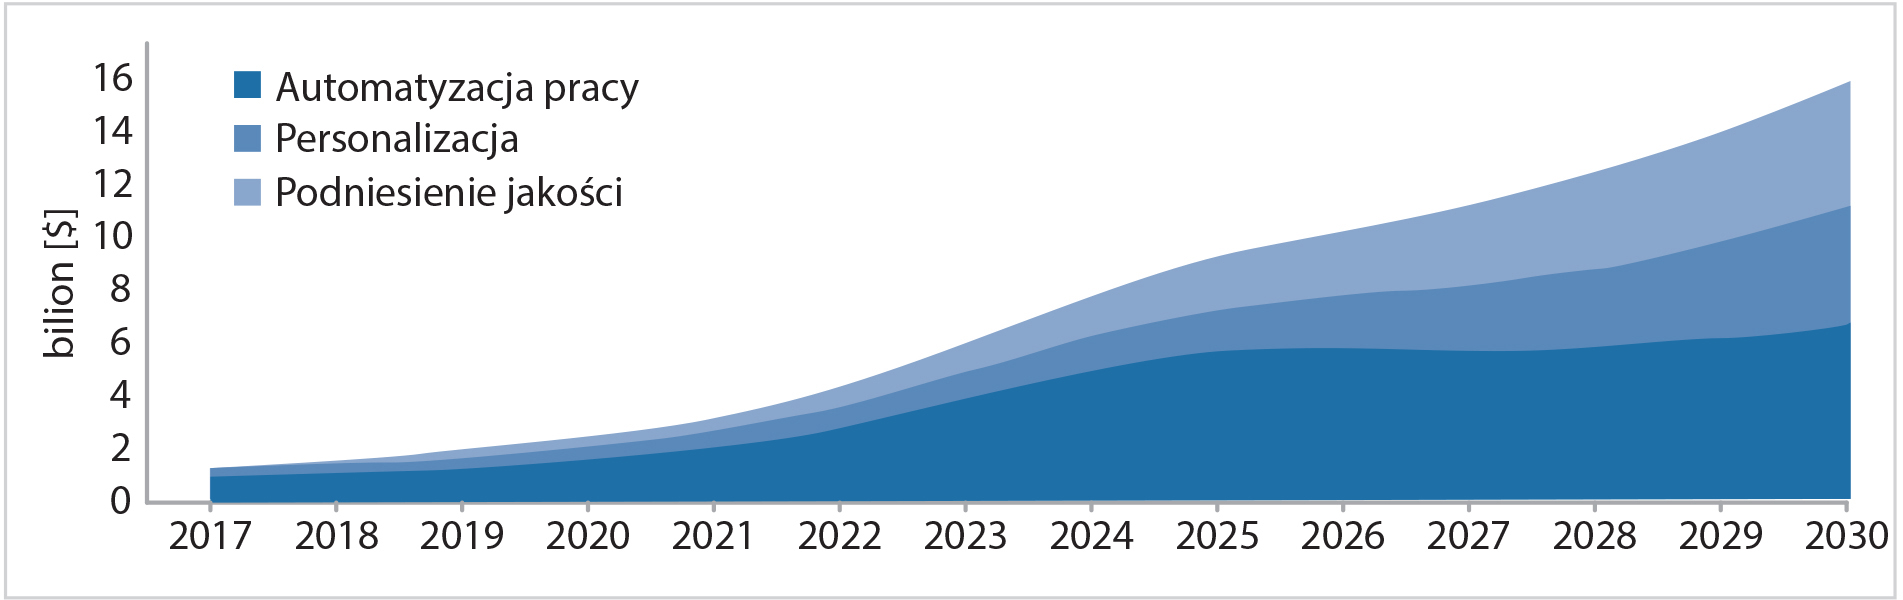
\includegraphics[width=1.0\textwidth]{figures/AI_w_radiologii.jpg}
	\caption{Kwota PKB wypracowana z udziałem rozwiązań opartych o SI aplikowanych na rynku Med-Tech (na podst. \cite{PWC}).}
	\label{MedTechGrowth}
\end{figure}

W pierwszej kolejności motorem zmian mają być aplikacje usprawniające generowanie raportów, następnie rozwiązania do personalizacji diagnostyki i narzędzia poprawiające jej jakość np. służące do uzyskania drugiej lub nawet pierwszej opinii. W rezultacie czas spędzony przez radiologa na pisanie raportu ma obniżyć się nawet o 90\%, przy niezmienionym lub nawet niższym współczynniku błędów diagnostycznych.

Metody, które według przewidywań mają najbardziej przyczynić się do rewolucji w radiologii, można podzielić na dwa rodzaje. Pierwszy to tzw. szeroka sztuczna inteligencja (ang. \textit{general Artificial Intelligence}), która docelowo ma odzwierciedlać złożony sposób zachowania się człowieka. Drugi rodzaj nazywany jest wąską Sztuczną Inteligencją (ang. \textit{narrow Artificial Intelligence}). Metody te mają zapewnić możliwie dobry efekt w wykonaniu konkretnego zadania np. klasyfikacji różnego rodzaju tkanek. 

W najbliższych latach przewidywane zmiany mają być efektem rozwoju metod wąskiej SI. Należy jednak podkreślić, że sam rozwój algorytmów ma już miejsce od ponad pół wieku. Krótki rys historyczny zawierający lata opracowania wybranych metod przedstawia się następująco: metoda regresji logistycznej -- rok 1958, ukryte modele Markova -- rok 1960, stochastyczny spadek wzdłuż gradientu -- rok 1960, Maszyna Wektorów Nośnych -- rok 1963, algorytm k-najbliższych sąsiadów -- rok 1967, wielowarstwowe sieci neuronowe -- lata 70-te ubiegłego wieku, algorytm EM (od ang. \textit{Expectation Maximization}) -- rok 1977, drzewa decyzyjne -- rok 1986, Q-learning -- rok 1989, lasy losowe -- rok 1995 oraz głębokie sieci neuronowych powstające \linebreak od lat 90-tych. 

W szczególności rozwój tych ostatnich został silnie przyspieszony z wykorzystaniem nowych architektur obliczeniowych takich jak akceleratory GPGPU (od ang. \textit{General-Purpose Computing on Graphics Processing Units}), czy TPU (od ang. \textit{Tensor Processing Unit}). Przede wszystkim uzyskano możliwość szybkiego testowania \linebreak i optymalizacji architektur zawierających miliony parametrów. W rezultacie dokładność realizacji przez współczesne metody bazujące na głębokich sieciach neuronowych, wybranych, praktycznych zadań, osiągnęła możliwości ludzkiej percepcji. 

\begin{figure}[h]
	\centering
	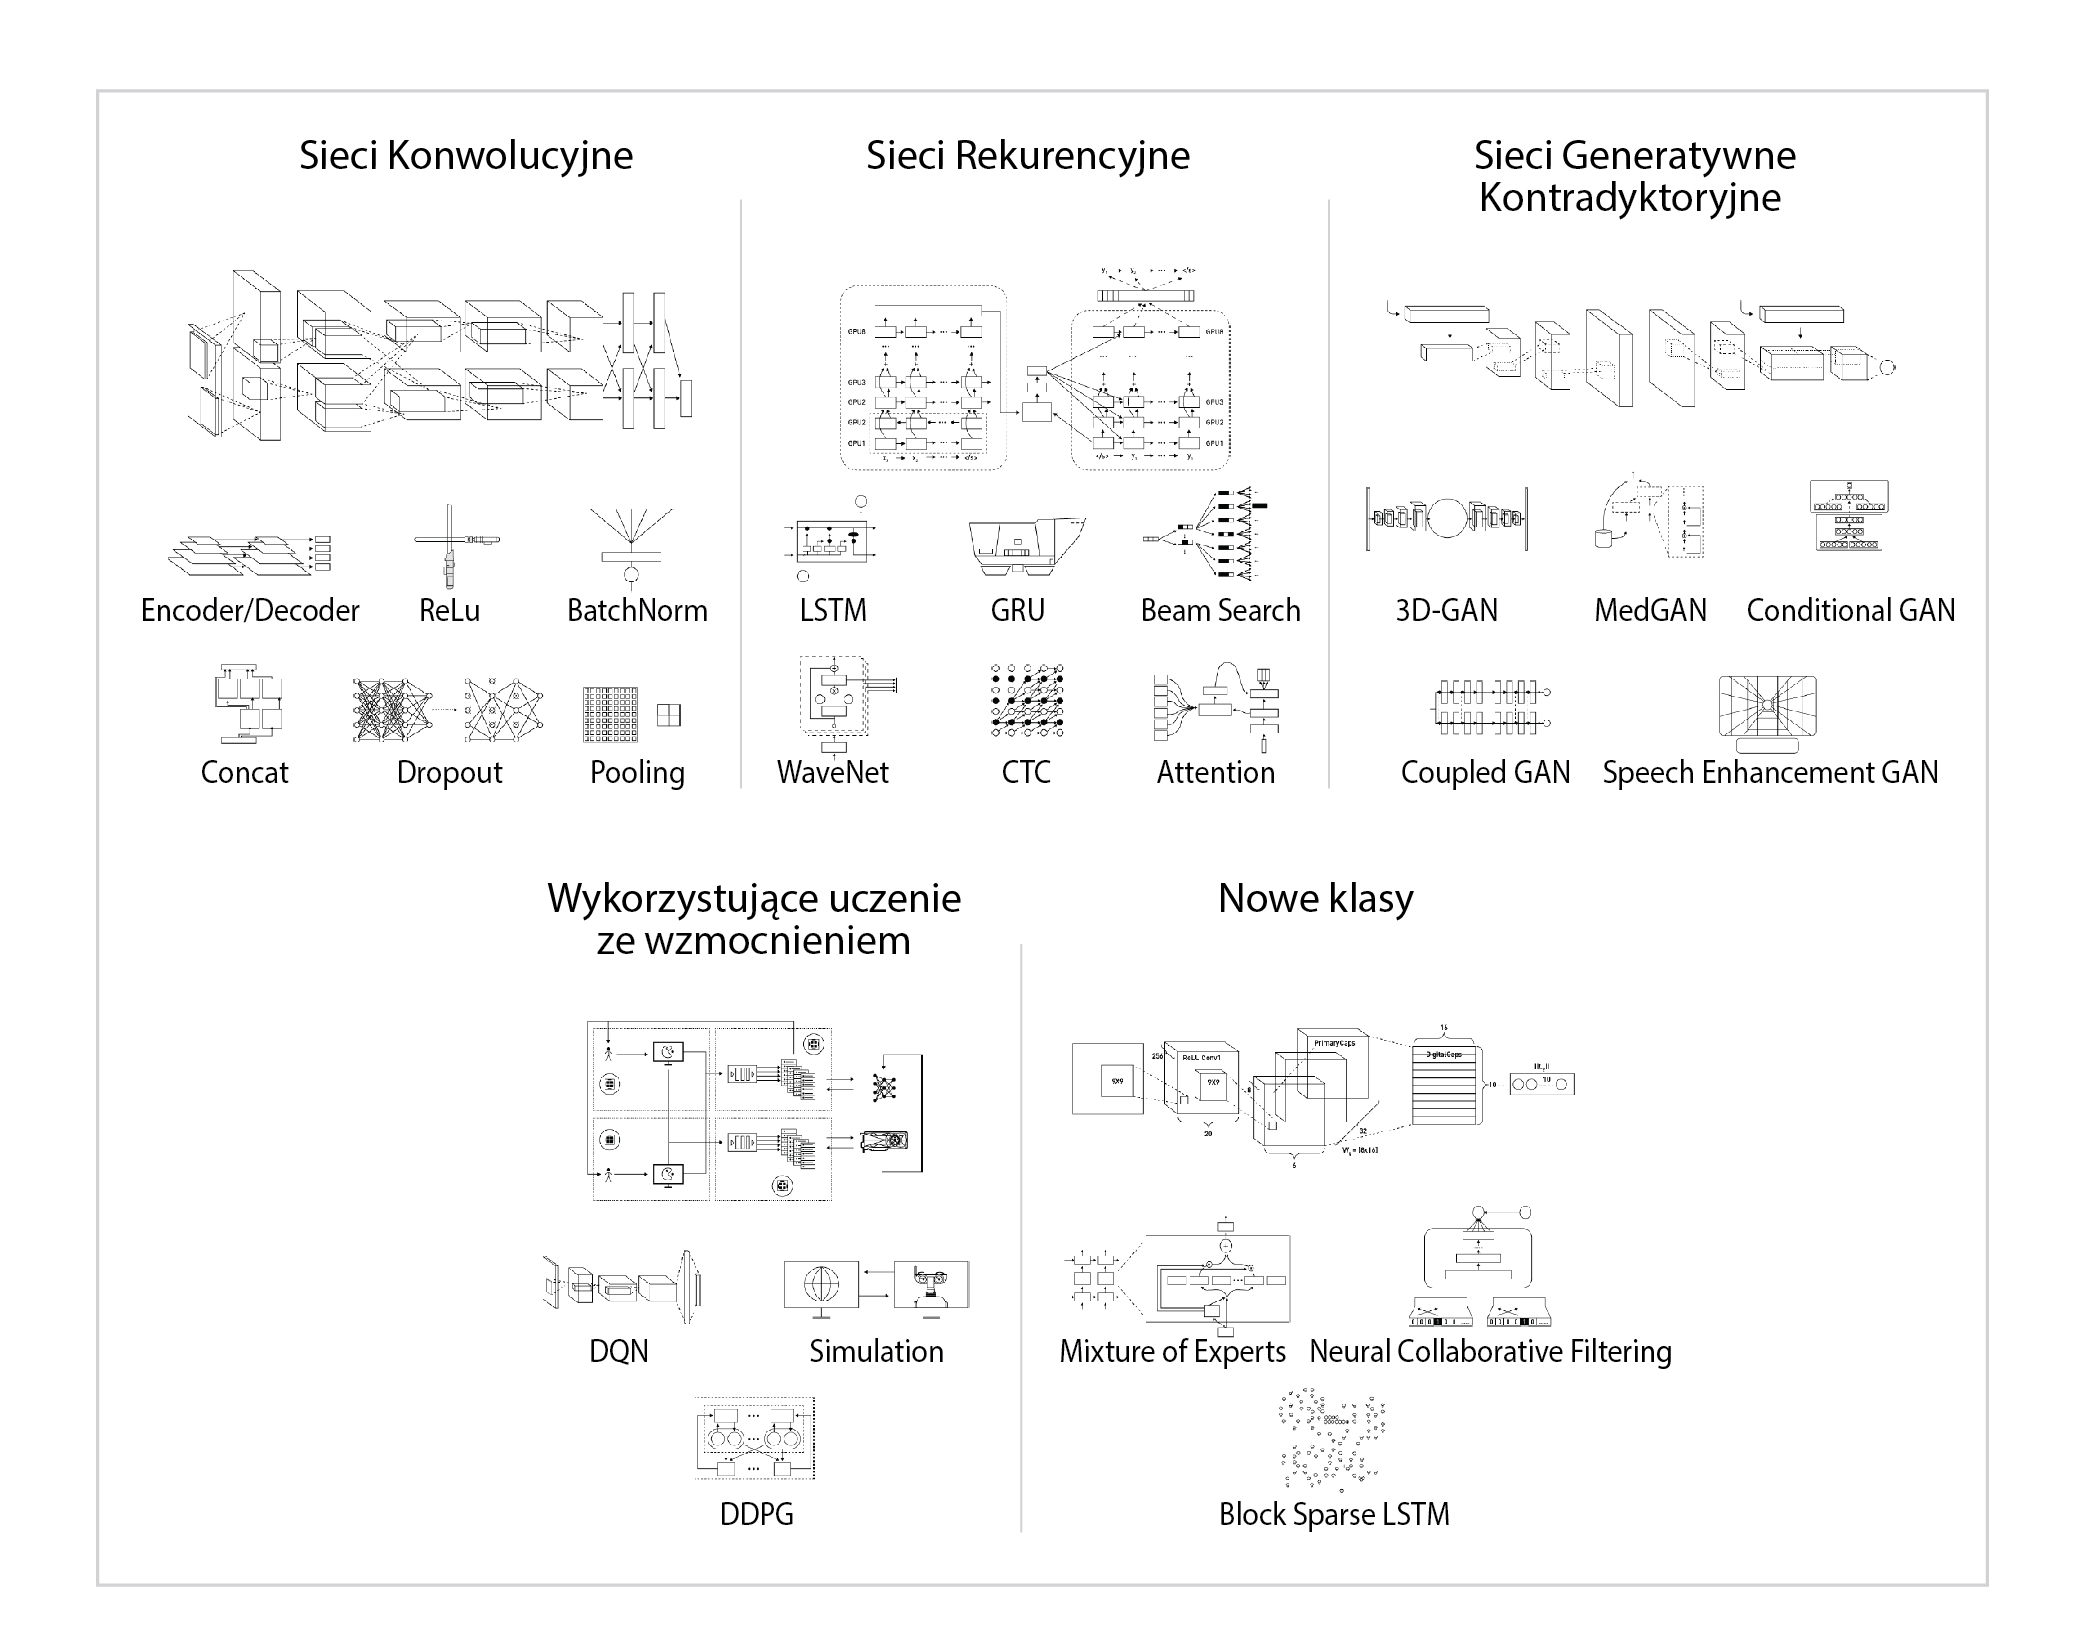
\includegraphics[width=1\textwidth]{figures/rodzajeSieciNeuronowych.png}
	\caption{Podział przedstawiający różne rodzaje współczesnych architektur głębokich sieci neuronowych.}
	\label{DLcambrianExplosion}
\end{figure}

Wśród głębokich sieci neuronowych wyróżnić można konwolucyjne sieci neuronowe stosowane najczęściej do przetwarzania obrazów, generatywne sieci kontradyktoryjne stosowane najczęściej do generowania danych, rekurencyjne sieci neuronowe stosowane najczęściej do rozpoznawania sekwencji, sieci wykorzystujące uczenie \linebreak ze wzmocnieniem do modelowania procesów decyzyjnych i szereg nowych klas jak sieci kapsułowe. Mnogość architektur (zob. Rys. \ref{DLcambrianExplosion}), powoduje, że na licznych konferencjach czy w publikacjach popularnonaukowych obecny stan rozwoju nazywany jest \textit{eksplozją kambryjską sieci neuronowych}. 


Z uwagi na fakt wykorzystania w radiologii w głównej mierze danych obrazowych, to właśnie konwolucyjne sieci neuronowe znajdują tu najczęstsze zastosowanie. Sieci te mają unikalną cechę umożliwiającą przekształcenia informacji obrazowej w numerycznie opisaną klasę przynależności. W szczególności, jak wskazują statystyki przedstawione na konferencji NVIDIA GTC w 2018 roku przez naukowców z niemieckiego centrum badań nad rakiem (DKFZ od niem. \textit{Deutsches Krebsforschungszentrum}), w około 71\% przypadków prace dotyczą automatycznego wydzielania struktur anatomicznych, w 12\% ich klasyfikacji, w 6\% samej detekcji (czy poszukiwane zjawisko znajduje się w danych) a w 3\% oceny postępu w leczeniu i monitoringu pacjentów. Pozostałe zadania jak np. lokalizacja struktur, czy strukturyzacja danych przyjmują wartości poniżej 2\%.

W tej pracy, sieci konwolucyjne zostały wykorzystane do realizacji metody komputerowego wspomagania radiologa w zadaniu monitorowania pacjentów w trakcie rehabilitacji po przebytym urazie całkowitego zerwania ścięgna Achillesa. Zgodnie \linebreak z przedstawionymi powyżej statystykami, prace należą zatem do wąskiej grupy oceny leczenia i monitoringu. Ze względu na charakter obecnie realizowanych badań, stanowią nowatorskie podejście do przedmiotowego problemu i odpowiadają na istotne problemy w radiologii.


\chapter{Cel i przebieg pracy}

Wyniki pracy zostały wykorzystane do realizacji projektu START: "Wykorzystanie autologicznych mezenchymalnych komórek macierzystych w procesie regeneracji rekonstruowanego ścięgna Achillesa", finansowanego przez Narodowe Centrum Badań i Rozwoju z krajowego programu STRATEGMED1. Celem całego projektu było opracowanie nowych nieinwazyjnych technik obrazowania oraz metod monitorowania procesu regeneracji tkanek oraz ocena szybkości gojenia się ścięgna Achillesa. \linebreak W ramach tych prac powstała koncepcja automatyzacji procesu monitorowania gojenia się ścięgna przy pomocy metod przetwarzania obrazów i sztucznej inteligencji. Biorąc pod uwagę przedstawioną dalej budowę głębokich sieci neuronowych i ekstrahowane przez nie cechy, założono, że będą one skuteczne do oceny procesów patofizjologicznych widocznych w obrazowaniu medycznym takich jak gojenie tkanki miękkiej, co stanowi hipotezę tej pracy.

W ramach weryfikacji hipotezy, za cel główny autor tej pracy postanowił obrać opracowanie automatycznej metody oceny gojenia się ścięgna Achillesa, bazującej na fuzji danych z wykorzystaniem głębokich sieci neuronowych. Jako dane wejściowe postanowiono wykorzystać dane z Rezonansu Magnetycznego (RM), który jest rutynowo stosowany do obrazowania tkanek miękkich i z uwagi na podstawy fizyczne jest też dobrym wyborem do monitorowania gojenia tkanek, zwłaszcza z uwagi na zmiany w ich ukrwieniu podczas tego procesu. Wedle najlepszej wiedzy autora jest to pierwsza próba automatyzacji oceny gojenia się ścięgna Achillesa widocznego w obrazowaniu medycznym RM. Stąd konieczność zrealizowania celów pobocznych, które stanowią:
\begin{enumerate}[noitemsep,nolistsep]
	\item Wybór efektywnego kosztowo i czasowo protokołu badania bazującego na technikach obrazowania medycznego, a dokładniej Rezonansu Magnetycznego.
	\item Przetestowanie różnego rodzaju podejść związanych ze szkoleniem głębokich sieci neuronowych.
	\item Porównanie wyników oceny nowej metody z wynikami klasyfikacji bazującej na danych z ultrasonografii.
	\item Porównanie wyników oceny nowej metody z oceną funkcjonalną, rutynowo stosowaną do wspomagania rehabilitacji po urazie ścięgna.
\end{enumerate}

W celu uporządkowanego i zrozumiałego przedstawienia podłoża oraz wyników badań, w pracy wprowadzono podział na Rozdziały. Po wstępie i opisie celu pracy, w Rozdziale 3 zostały opisane współczesne metody monitorowania gojenia się ścięgna Achillesa. Rozdział ten rozpoczyna się od omówienia podstaw anatomicznych, biomechanicznych oraz dynamiki procesu gojenia się przedmiotowego ścięgna. Następnie przedstawiony jest szczegółowy opis badań obrazowych i biomechanicznych wykorzystywanych do oceny stanu rehabilitującego się pacjenta. W Rozdziale 4, omówione zostały szczegółowo konwolucyjne sieci neuronowe, które posłużyły jako rdzeń opracowanego rozwiązania. W szczególności, w opisie uwzględniono zarys historyczny pozwalający zrozumieć etapy rozwoju współczesnych sieci, problemy z budową efektywnych modeli na bazie sieci neuronowych oraz osiągnięcia w tym zakresie wraz z omówieniem sukcesów w zastosowaniach w medycynie. W Rozdziale 5 zaprezentowano nowatorską metodę automatycznej oceny procesu gojenia się ścięgna Achillesa. Co istotne, omówiono unikalny zbiór danych oraz wzorzec odniesienia, dzięki którym możliwa była realizacja przewidzianych badań i walidacja metody. Przedstawiono również eksperymenty wykorzystane do doboru komponentów i parametrów ostatecznego modelu oraz finalny wynik funkcjonowania opracowanego algorytmu. W Rozdziale 6 opisano zestawienie wyników metody z wynikami oceny realizowanej przez inne podejścia. W szczególności porównano przedmiotową metodę z metodą uczącą się explicite modelować ocenę radiologa, opracowaną również pod kierownictwem autora tej pracy w ramach pobocznych działań. Następnie zaprezentowano zestawienie z wynikami metody działającej w oparciu o dane \linebreak z ultrasonografii, również opracowanej pod kierownictwem autora tej pracy. Finalnie, porównano wyniki z oceną biomechaniczną realizowaną standardowo przez fizjoterapeutów. Całość pracy zakończono podsumowaniem przedstawionym w Rozdziale~7.   




\chapter{Monitorowanie procesu gojenia ścięgna Achillesa}
\section{Ścięgno Achillesa}
Ścięgno Achillesa, nazywane również ścięgnem piętowym, jest największym i zarazem wytrzymującym największe obciążenia ścięgnem występującym w ciele ludzkim. Stanowi wspólne zakończenie mięśnia trójgłowego łydki, w którego skład wchodzą dwie głowy mięśnia brzuchatego i mięsień płaszczkowaty. Całość struktury zlokalizowana jest w tylnym, powierzchownym przedziale łydki, co zobrazowano \linebreak na Rysunku \ref{muscle_structure}.  
\begin{figure}[h!]
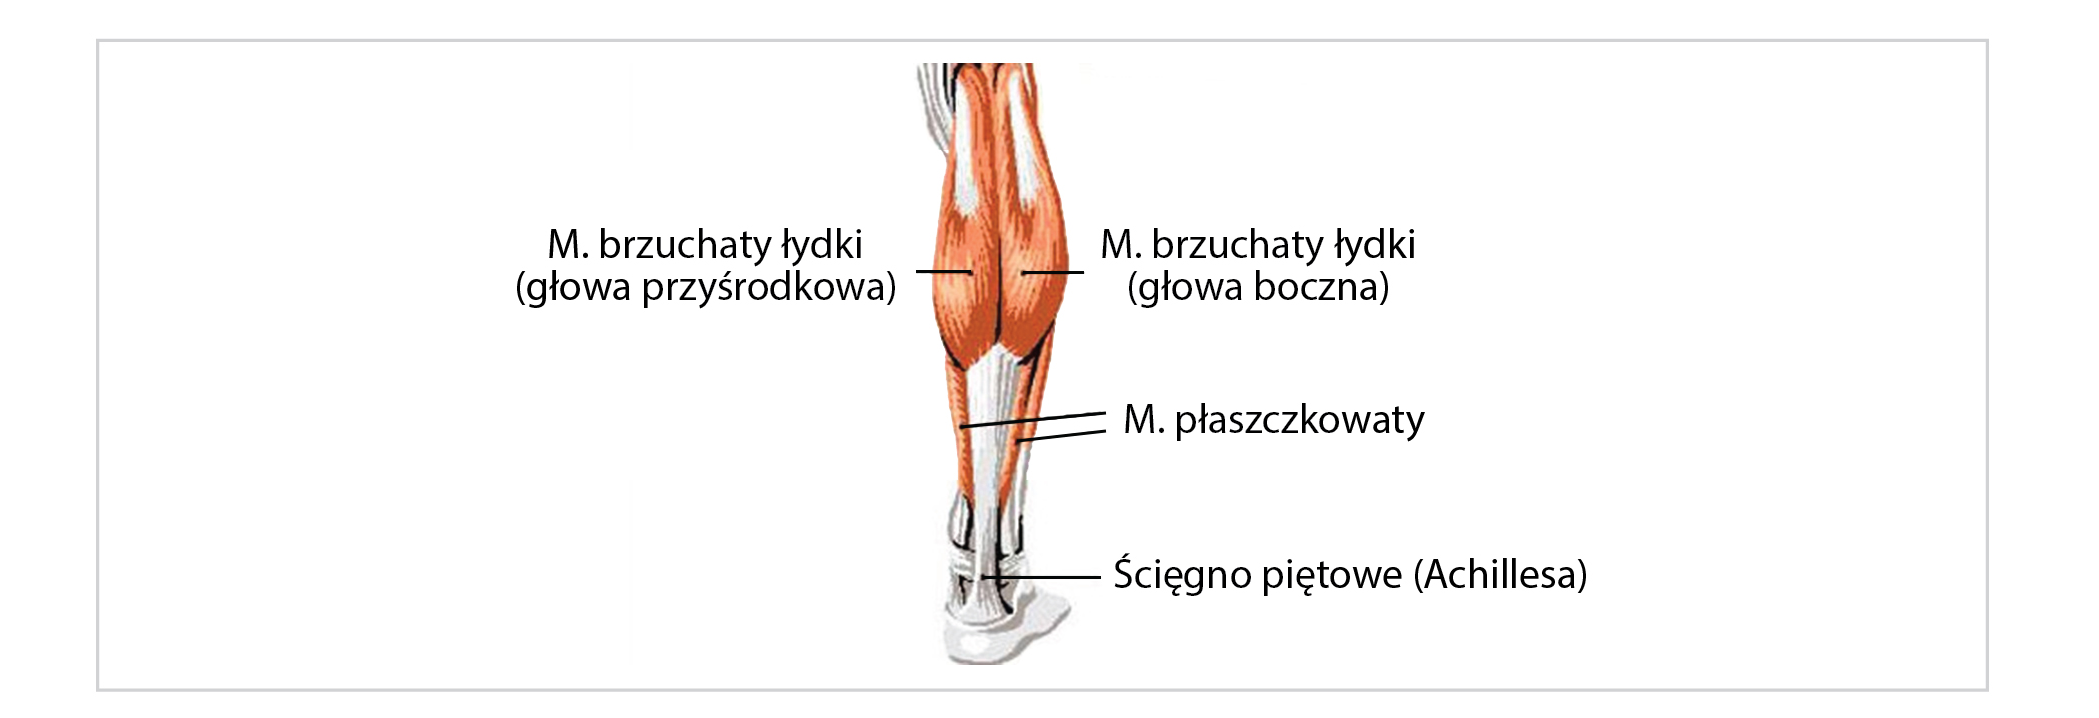
\includegraphics[width=1\textwidth]{figures/muscleStructure.png}
\caption{Lokalizacja mięśnia trójgłowego łydki wraz ze ścięgnem Achillesa (na podst. \cite{Doral2010}).}
\label{muscle_structure}
\end{figure}
\newpage
Procesy patofizjologiczne zachodzące po urazie ścięgna są ściśle związane z jego anatomią, biomechaniką, typem urazu i czynnikami jemu sprzyjającymi. Wszystkie te aspekty mają wpływ na możliwość monitorowania procesów gojenia się ścięgna \linebreak i jego wspomagania. Dlatego zostaną szczegółowo omówione w kolejnych punktach. 

\subsection{Anatomia}
\label{anatomia}

Z obu głów (brzuśców) mięśnia brzuchatego łydki wyrasta jedno szerokie, płaskie pasmo, które jest początkiem części brzuchatej ścięgna Achillesa. Następnie ścięgno to łączy się z włóknami pochodzącymi od mięśnia płaszczkowatego, które układają się stycznie do wcześniej powstałej struktury. Podążając w dół łydki, kształt ścięgna Achillesa ulega stopniowemu zwężeniu i zaokrągleniu, aż do punktu o minimalnej szerokości (około 4 cm nad przyczepem dolnym -- za \cite{Doral2010}). W rejonie samego przyczepu, znajdującego się na guzie piętowym, ścięgno ponownie jest płaskie i szerokie.

Średnia długość ścięgna Achillesa to 15 cm (zakres to: 11 -- 26 cm). Średnia szerokość w rejonie początku wynosi 6,8 cm (4,5 -- 8,6 cm), w rejonie zwężenia \linebreak to 1,8 cm (1,2 -- 2,6 cm), a w miejscu przyczepu dolnego 3,4 cm (2,0 -- 4,8 cm) \cite{Doral2010, KoivunenNiemel1995}.

Ścięgno jest zbudowane z tkanki łącznej, a dokładniej mówiąc z tkanki łącznej właściwej zbitej. Składa się w przeważającej części z \textit{istoty międzykomórkowej} (nazywanej też \textit{macierzą międzykomórkową}) zbudowanej z istoty podstawowej (ang. \textit{ground substance}) oraz włókien. Dopełnienie struktury stanowią komórki takie jak fibroblasty, komórki tuczne, komórki plazmatyczne, histiocyty i komórki napływowe. 

Istota podstawowa jest rodzajem żelu wiążącym duże ilości wody, włókien i komórek. Pełni ona rolę otoczki zapewniając możliwość transportu wody i substancji odżywczych do wnętrza struktury \cite{Sharma2006}, gdzie znajdują się komórki poukładane \linebreak w wąskie pasy leżące pomiędzy włóknami \cite{Maffulli2005}. Wśród włókien można wyróżnić trzy rodzaje: kolagenowe, siateczkowe i sprężyste.

Włókna kolagenowe i siateczkowe są zbudowane z fibrylarnego białka -- kolagenu, najczęściej występującego białka w organizmie człowieka, stanowiącego około 25\% wszystkich białek. Makrocząsteczki kolagenu składają się ze zwiniętych łańcuchów polipeptydowych tworzących helisy. Dotychczas zidentyfikowano 20 typów kolagenu różniących się od siebie szczegółową budową helisy. Kolagen typu I stanowi około 90\% masy wszystkich typów włókien i jest podstawowym budulcem włókien kolagenowych tworzących zazwyczaj wiązki o grubości 50--100 $\mu$$m$. Włókna siateczkowe zbudowane są natomiast w przeważającym stopniu z kolagenu typu III. Pozostałe typy kolagenu występują w znacząco mniejszym stopniu tworząc włókienka kolagenowe i siateczkowe o różnej grubości -- od 10 do 300 nm (por. \cite{sawicki2008histologia}).

Włókna sprężyste występują w postaci sieci i mają średnicę 0,2--10 $\mu$$m$. Zbudowane są z \textit{elastyny}, rozciągliwego i sprężystego białka. Dzięki temu, włókna te pod wpływem działania siły zewnętrznej mogą zwiększać swoją długość nawet o 50\% (za. \cite{sawicki2008histologia}). 

W zdrowym ścięgnie Achillesa widoczne są ściśle upakowane włókna sprężyste \linebreak i kolagenowe. Włókna kolagenowe stanowią 70\% masy suchego ścięgna i charakteryzują się hierarchiczną strukturą zobrazowaną na Rys. \ref{Achilles-histology}.  
\begin{figure}[h!]
	\centering
	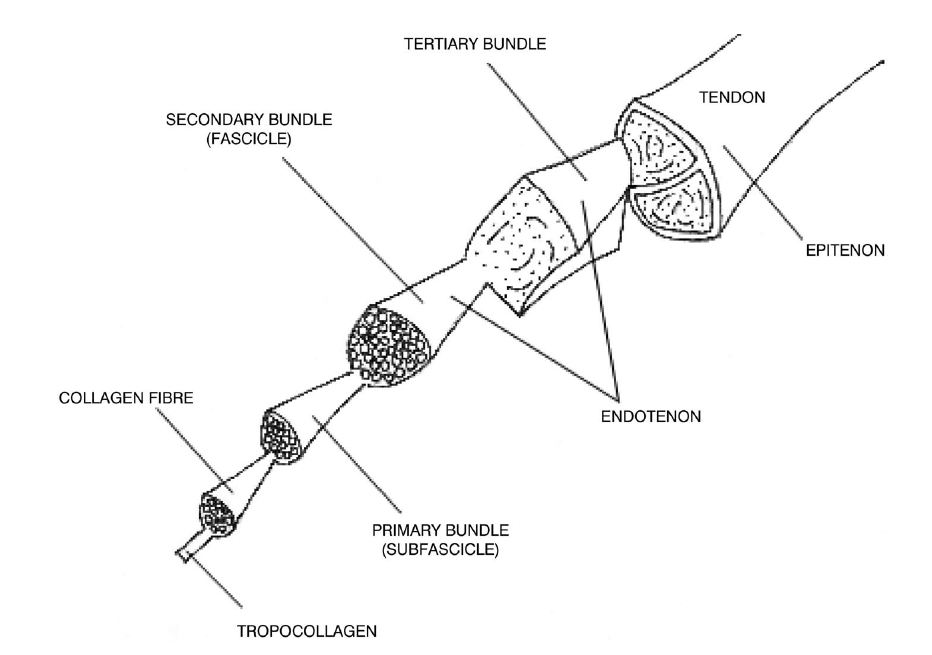
\includegraphics[width=1\textwidth]{figures/Achilles_hist.png}
	\caption{Schemat hierarchicznej budowy ścięgna Achillesa (na podst. \cite{Sharma2006}).}
	\label{Achilles-histology}
\end{figure}

Wyróżnić można: włókna, wiązki pierwszo, drugo i trzeciorzędowe \cite{Sharma2006}. W przeciwieństwie do innych ścięgien, ścięgno Achillesa nie posiada pochewki ścięgnistej, lecz jest otoczone ościęgnem utworzonym z tkanki łącznej włóknistej. Struktura \linebreak ta umożliwia ślizg wewnętrznych włókien, jest bogata w naczynia krwionośne i pełniąc funkcje transportowe jest bardzo ważnym elementem w procesie gojenia. 

Oprócz otaczającej tkanki łącznej, ścięgno czerpie źródło unaczynienia z brzuśców mięśni brzuchatego i płaszczkowatego oraz z połączenia kostno-ścięgnistego. Najsłabsze unaczynienie występuje na poziomie ok. 4-5 cm powyżej górnego brzegu kości piętowej (por. \cite{bochenek2016anatomia}).

Unerwienie rejonu ścięgna Achillesa zapewnia nerw piszczelowy, biegnący wzdłuż całego ścięgna, a także nerw łydkowy, który krzyżuje się ze ścięgnem w odległości 8,7--12,4 cm proksymalnie od guza piętowego (por. \cite{bochenek2016anatomia}). 

\subsection{Biomechanika}
\label{Biomechanika}
Zadaniem ścięgien jest transfer siły mięśniowej do układu szkieletowego. Pod względem mechanicznym ścięgno piętowe jest najwytrzymalszym ścięgnem całego ustroju. Dla przykładu podczas chodu maksymalne obciążenie ścięgna Achillesa wynosi 500 N, przy biegu jest to 9000 N, natomiast podczas wyskoku może sięgać 12000 N, co stanowi równoważność 12--15 krotnej masy ciała. Podobne obciążenia wytrzymuje tylko ścięgno właściwe rzepki \cite{Etiologia}.

Głównym zadaniem ścięgna Achillesa w trakcie prawidłowego chodu, biegu, czy wyskoku jest ruch \textit{zginania podeszwowego stopy}, a zatem wyprost powodujący wspięcie na palce. Takie zadanie implikuje zwiększone ryzyko nadmiernego napięcia, \linebreak a w konsekwencji przeciążenia, rozwój stanu zapalnego, a nawet uszkodzenia ścięgna \cite{Etiologia}.

Cały proces ruchu rozpoczyna się od centralnego układu nerwowego skąd wysyłane są impulsy nerwowe. Trafiają one do odpowiednich grup mięśniowych za pośrednictwem \textit{nerwu ruchowego}, struktury  przewodzącej impulsy wzbudzające proces skurczu mięśni. Na styku nerwu z komórką mięśniową znajduje się \textit{synapsa nerwowo-mięśniowa} (tzw. \textit{płytka motoneuronalna}). Do niej właśnie na skutek impulsu wydzielany jest neuroprzekaźnik -- \textit{acetylocholina}. W wyniku działania tej substancji następuje dalsze pobudzenie błony komórki mięśniowej i uwolnienie jonów wapnia Ca$^{2+}$. Cząsteczki aktywują białka kurczliwe tj. \textit{aktynę} i \textit{miozynę}, a także pośrednio wywołują produkcję w mięśniu \textit{adenozyno-5'-trifosforanu}, (\textit{ATP}), czyli substancji zapewniającej dostarczenie odpowiedniej energii chemicznej dla procesu.
\begin{figure}[h!]
	\centering
	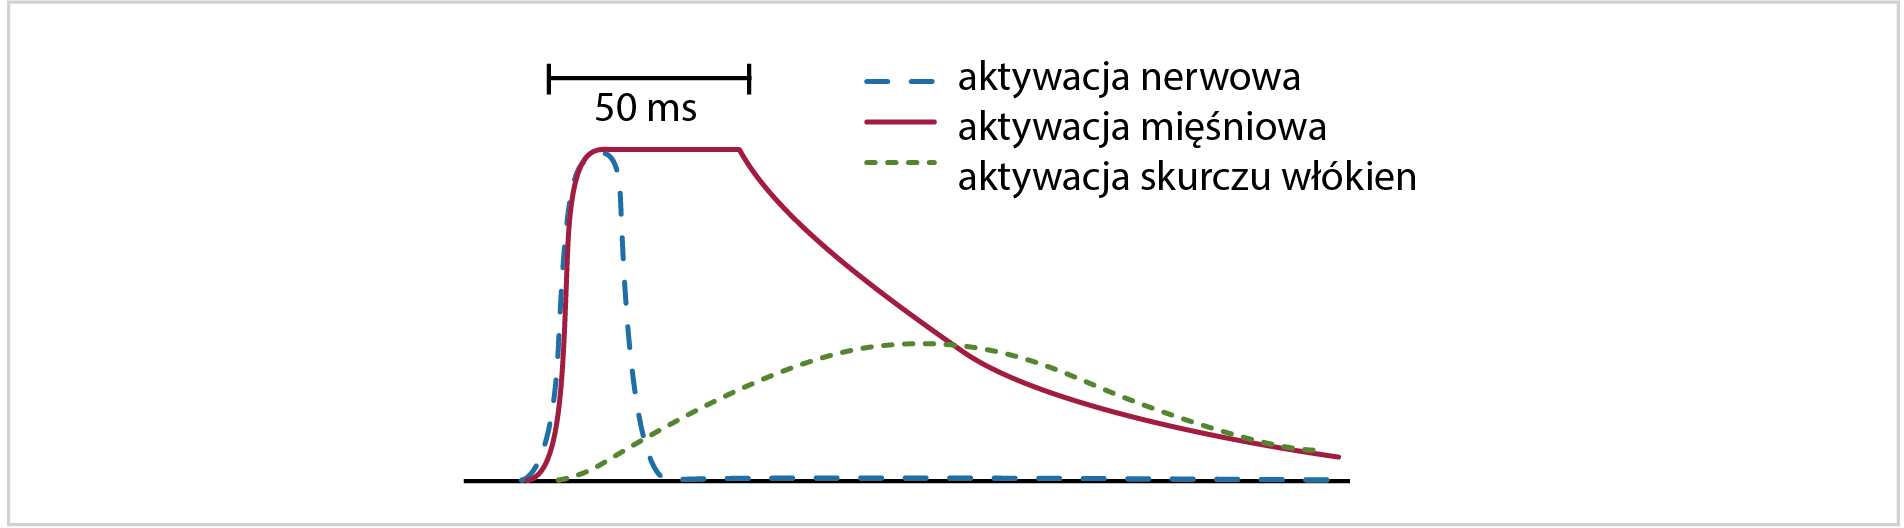
\includegraphics[width=1\textwidth]{figures/skurcz_miesni.png}
	\caption{Schemat generowania skurczu mięśni.}
	\label{muscle-excitements}
\end{figure}

Skurcz mięśni szkieletowych trwa 100--300 milisekund. Schemat czasów i orientacyjnych poziomów poszczególnych aktywacji, przedstawiono na Rys. \ref{muscle-excitements}. Jak wcześniej zaznaczono, siła wygenerowana przez skurcz jest przekazywana za pomocą ścięgien do układu szkieletowego. Dobrym przybliżeniem tego procesu jest \textit{model Hill'a} \cite{Hill1938}. Jego warianty, których przykłady opisane są np. w \cite{Perreault2003} służą obecnie w wielu rozwiązaniach do symulacji pracy układu mięśniowo-szkieletowego. Przykład z popularnego rozwiązania OpenSim rozwijanego na Uniwersytecie Stanforda znajduje się na Rys. \ref{hill-model}.
\begin{figure}[h!]
	\centering
	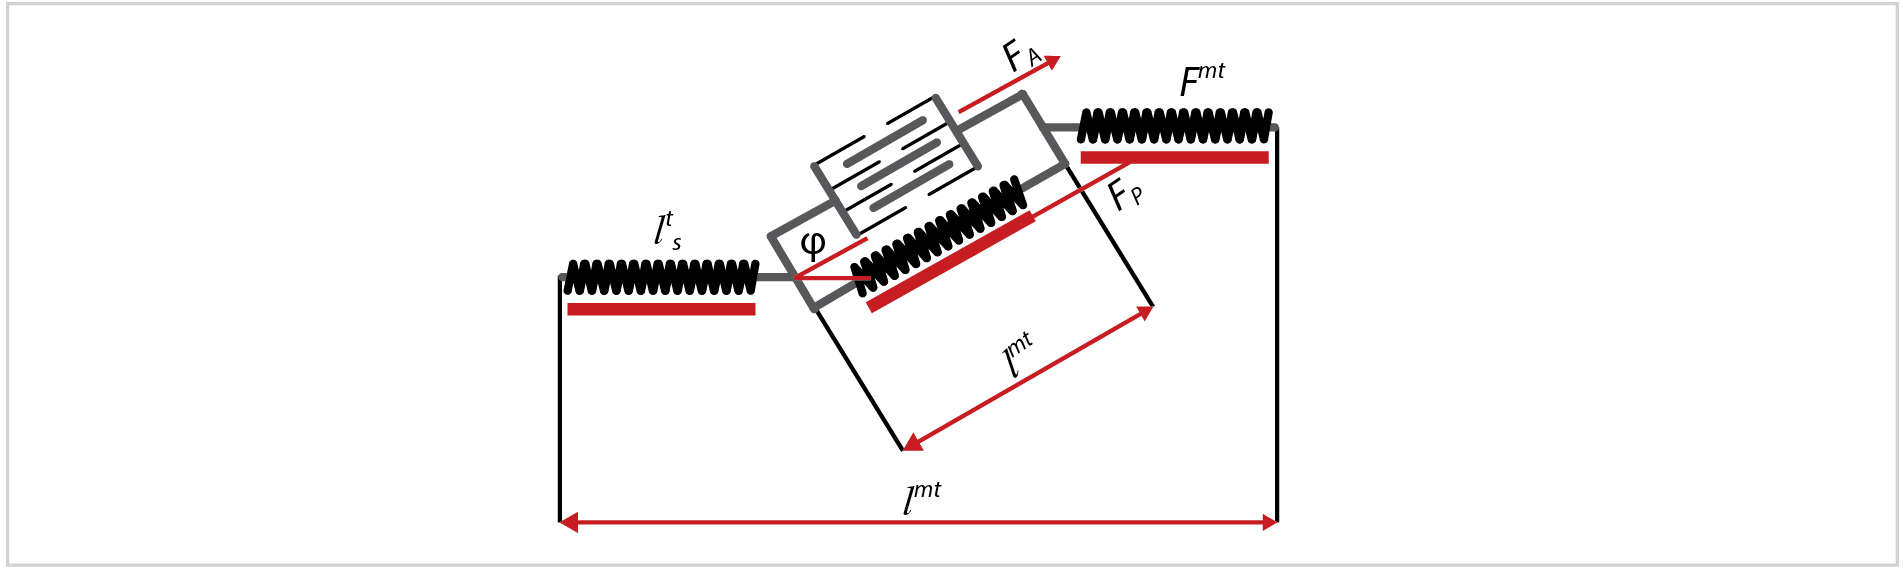
\includegraphics[width=1\textwidth]{figures/Hill.png}
	\caption{Schemat modelu typu Hilla stosowany w oprogramowaniu OpenSim (na podst. \cite{Romero2016}).}
	\label{hill-model}
\end{figure}

Na podanym schemacie $F_A$ oznacza siłę wywoływaną skurczem mięśni, $F_P$ \linebreak to pasywna siła odpowiadająca za bezwładność tkanki miękkiej w mięśniu, a $F^{mt}$ to wynikowa siła przekazywana przez ścięgno, która zależy od długości ścięgna $l_t$ \linebreak i kąta $\phi$ pomiędzy ścięgnem a mięśniem. To właśnie na skutek przekroczenia wartości granicznej siły $F^{mt}$ dochodzi najczęściej do urazu ścięgna Achillesa. 

\subsection{Urazy i czynniki im sprzyjające}

Uszkodzenie ścięgna Achillesa jest jednym z najczęściej występujących urazów układu mięśniowo-szkieletowego. Przykładowo, dla społeczeństwa amerykańskiego, urazy te występują u 18-tu na 100.000 osób rocznie. Ryzyko ponownego zerwania ścięgna wynosi 20--40\% (zob. \cite{EpidemiologyUS}). 

Można wyróżnić dwa mechanizmy uszkodzenia ścięgna Achillesa: 
\begin{enumerate}[noitemsep,nolistsep]
	\item Uraz bezpośredni, do którego zaliczyć można urazy otwarte spowodowane np. przecięciem ostrym przedmiotem takim jak szkło oraz urazy zamknięte spowodowane nagłym uderzeniem w napięte ścięgno.
	\item Uraz pośredni, znacznie częściej spotykany niż uraz bezpośredni. Powstaje \linebreak on w wyniku nagłego, silnego skurczu mięśnia połączonego często z innymi siłami zewnętrznymi towarzyszącymi np. podczas upadku.
\end{enumerate}
O ile uraz bezpośredni jest najczęściej następstwem nieszczęśliwego wypadku, o tyle urazy pośrednie mają swoją przyczynę w rodzaju wykonywanych czynności oraz predyspozycji danej osoby. 

Zazwyczaj do urazów pośrednich dochodzi podczas uprawiania sportu. Dotyczy to zwłaszcza sportu rekreacyjnego (około 70\% przypadków). W tym obszarze \linebreak aż 75\% przypadków przytrafia się mężczyznom w przedziale wiekowym wahającym się od 30-tego do 50-tego roku życia. Statystyki te mają związek z obniżeniem poziomu ukrwienia ścięgna po 30-tym roku życia oraz sporadycznym, ale nadmiernym obciążaniem ścięgna przez osoby niewytrenowane (zob. \cite{Etiologia}). Ponadto, istotne dane zebrane w duńskim społeczeństwie, przeanalizowane w \cite{Ganestam2015}, pokazują również, że wzrost całościowej liczby przedmiotowych urazów, wynika także z faktu starzenia się społeczeństwa oraz zwiększonej liczby zerwań w grupie wiekowej po 50-tym roku życia. 

Dyscypliny sportowe, podczas których najczęściej dochodzi do urazu ścięgna Achillesa to: piłka nożna, siatkówka, tenis, taniec, koszykówka, skoki, biegi, piłka ręczna, aerobic, pływanie, ping-pong, biegi, narciarstwo, balet. Proporcje są naturalnie uzależnione od popularności danego sportu w konkretnym kręgu ludzi. \linebreak Na Rys. \ref{rupture} zobrazowano udział poszczególnych dyscyplin w urazach ścięgna Achillesa dla społeczeństwa amerykańskiego. 
\begin{figure}[h!]
	\centering
	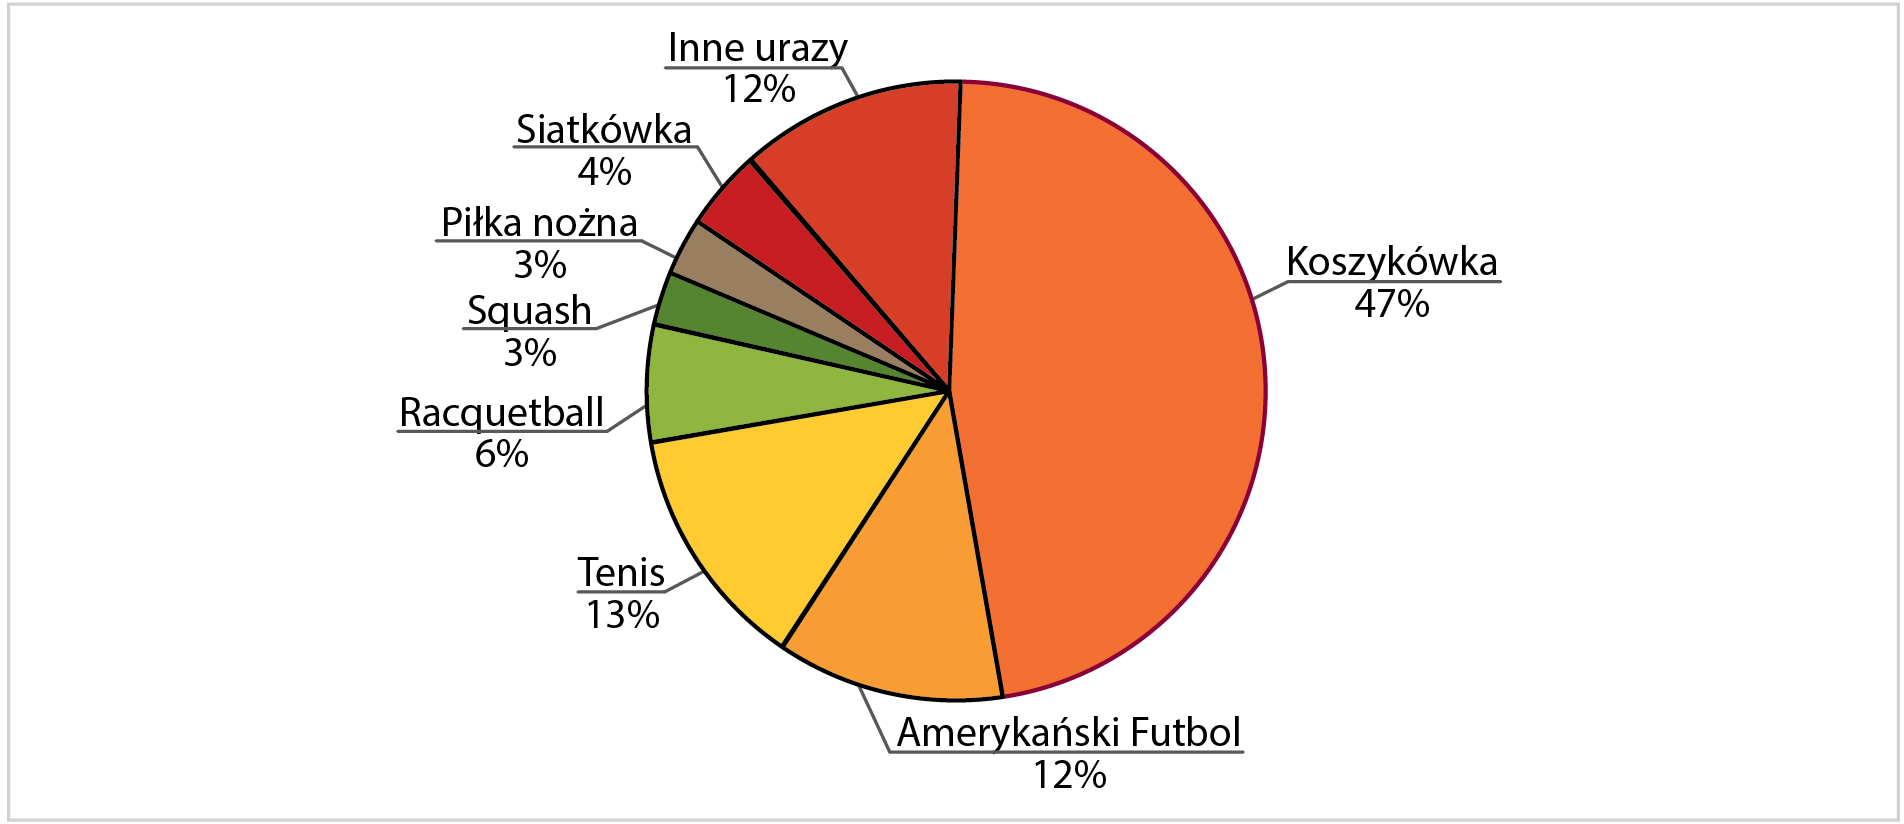
\includegraphics[width=1\textwidth]{figures/Achilles_zerwanie.png}
	\caption{Wykres przedstawiający proporcje występowania urazu ścięgna Achillesa w różnych dyscyplinach sportowych na przykładzie amerykańskiego społeczeństwa (na podst. \cite{EpidemiologyUS}).}
	\label{rupture}
\end{figure}

\newpage
W Stanach Zjednoczonych sportem największego ryzyka jest koszykówka (47\%), natomiast w Europie jest to piłka nożna (około 60\%). Według szacunków przedstawionych w \cite{CHIRALI2014211} uraz ścięgna Achillesa stanowi 5--10\% wszystkich urazów atletycznych.

Powszechnie uważa się, że zdrowe ścięgno piętowe jest bardzo ciężko zerwać \linebreak z uwagi na jego dużą wytrzymałość. Wycinek ścięgna o przekroju 1 cm$^2$ jest w stanie utrzymać masę 500--1000 kg \cite{Maquirriain2011}. Do urazów dochodzi zatem najczęściej, gdy ścięgno jest zmienione patologicznie. Czynniki powodujące osłabienie ścięgna Achillesa można podzielić na: zewnętrzne i wewnętrzne.

Do czynników wewnętrznych należy zaliczyć:
\begin{itemize}[noitemsep,nolistsep]
	\item zmiany degeneracyjne -- inwolucyjne (zwłaszcza przy wieku powyżej 30-tu lat), na podłożu stanów zapalnych (w szczególności przewlekłych), związane z mikrourazami;
	\item nadmierne przeciążenia -- nieprawidłowa aktywność fizyczna;
	\item choroby metaboliczne i układowe -- takie jak np. toczeń trzewny, dna moczanowa, nadczynność tarczycy, gruczolaki przysadki mózgowej, reumatoidalne zapalenie stawów, kolagenozy;
	\item odchylenia anatomiczne i biomechaniczne -- anomalie takie jak: piszczel szpotawa, stopa koślawa, stopa płasko-koślawa, niestabilność stawu skokowego, koślawość lub szpotawość tyłostopia, osłabienie i przykurcz mięśni okołostawowych, ograniczenie ruchomości stawu skokowo-goleniowego i skokowo-piętowego, nierówność kończyn dolnych, nieprawidłowy stereotyp chodu, pogłębione krzywizny kręgosłupa, zespół ciasnoty przedziałów powięziowych w obrębie przedziału tylnego goleni;
	\item zaburzenia naczyniowe -- związane ze schorzeniami takimi jak: hiperlipidemia, cukrzyca lub wywołane nadmiernym paleniem tytoniu;
	\item inne, takie jak: dysbalans mięśniowy, zaburzenia proprioceptywne, niepełne wyleczenie poprzednich obrażeń, przyjmowanie kortykosteroidów.
\end{itemize}

Do czynników zewnętrznych zaliczyć można:
\begin{itemize}[noitemsep,nolistsep]
	\item błędy w metodyce prowadzenia zajęć -- np. nadmierny trening, trening jednostronny, trening wszechstronny z przewagą intensywności nad wytrzymałością czynnościową aparatu więzadłowo-stawowo-mięśniowego, chęć nadrobienia zaległości treningowych;
	\item nagła zmiana dyscypliny sportowej lub aktywności rekreacyjnej;
	\item inne takie jak: nieodpowiednia nawierzchnia, niekorzystne warunki pogodowe, nieodpowiednie obuwie, zbyt krótkie przerwy między zawodami lub treningami.
\end{itemize}

Obecnie ustalenie jednej optymalnej metody leczenia dla każdego rodzaju uszkodzenia ścięgna Achillesa nie jest możliwe. Wybór uwarunkowany jest poziomem \linebreak i stopniem zniszczenia ścięgna, stanem zdrowia pacjenta oraz kwalifikacjami, doświadczeniem i możliwościami danego ośrodka. W kolejnym punkcie omówione zostaną współczesne metody leczenia tego schorzenia, natomiast w Rozdziale \ref{NewMethod} zaprezentowana zostanie nowa metoda monitorowania procesu gojenia się ścięgna Achillesa, która może być wykorzystana do optymalizacji rehabilitacji opisanego problemu. 

\subsection{Fazy gojenia, leczenie i rehabilitacja}
\label{gojenie}

Proces gojenia się ścięgna Achillesa można podzielić na trzy zachodzące na siebie etapy. W pierwszej kolejności dochodzi do stanu zapalnego. Jest to tzw. \textit{faza zapalna} (ang. \textit{inflammatory phase}), która trwa przez pierwszy tydzień gojenia się. Następnie występuje \textit{faza proliferacji} (ang. \textit{proliferative phase}), trwająca od drugiego \linebreak do szóstego tygodnia. Cały proces kończy się \textit{fazą przebudowy} (ang. \textit{remodeling phase}), która może trwać nawet do 18 miesiąca po urazie \cite{Sharma2006, Yang2013, Docheva2015, CMC}. 

Faza zapalna zaczyna się od razu po wypadku. W miejscu urazu tworzy się skrzep krwi oraz uwalniane są prozapalne substancje chemiczne, cytokiny, które \linebreak w znaczącym stopniu odpowiadają za proces aktywacji i migracji komórek zapalnych z otoczenia do miejsca zapalenia \cite{Lin2004}. Komórki te, a dokładniej mówiąc leukocyty \linebreak i makrofagi, rozpoczynają \textit{fagocytozę}, czyli proces mający na celu usunięcie obumarłej tkanki oraz skrzepu \cite{Yang2013, Beredjiklian2003, Lin2004}. Symultanicznie dochodzi do aktywacji i selekcji \textit{tenocytów} (komórek ścięgna), które rozpoczynają odbudowę włókien ścięgna \cite{Yang2013} oraz inicjują drugą fazę całego procesu.

W fazie proliferacji poziom komórek zapalnych zaczyna spadać. Czynniki wzrostu, uwalniane m.in. przez makrofagi, nasilają migrację i rozmnażanie tenocytów wokół miejsca urazu. Skutkiem tego procesu jest wytworzenie nowych włókien kolagenu typu III. Nowopowstałe struktury są początkowo zorientowane losowo \cite{Yang2013, Beredjiklian2003, Docheva2015}, dlatego rozpoczyna się trzecia faza mająca na celu odtworzenie struktury zdrowego ścięgna.

W trakcie trwania ostatniej fazy, nazywanej również \textit{remodelingiem}, włókna kolagenu typu III zastępowane są kolagenem typu I. Pod wpływem naprężeń struktura włókien zmienia się i wyrównuje zgodnie z kierunkiem występujących sił \cite{Yang2013}. Włókna pracujące niezgodnie z przewidzianym ruchem ulegają zerwaniu i fagocytozie, \linebreak a te które wspomagają zadany ruch ulegają wzmocnieniu. 

Pomimo całego wyżej opisanego procesu, ścięgno wygojone odbiega strukturą od ścięgna zdrowego. Charakteryzuje się nawet dwukrotnie zwiększoną powierzchnią przekroju osiowego oraz podatnością na ponowne zerwania z uwagi na zmniejszoną odporność na obciążenia. 

Uraz ścięgna Achillesa można leczyć zachowawczo lub operacyjnie. Zachowawcze leczenie stosuje się najczęściej przy częściowym uszkodzeniu ścięgna lub u osób, które mają przeciwwskazania do leczenia chirurgicznego. Stosowane jest wówczas unieruchamianie kończyny np. poprzez włożenie w but ortopedyczny lub gips. Dodatkowo można również stosować preparaty z komórek macierzystych i czynników wzrostu \cite{CMC}. Wybór leczenia zachowawczego wiąże się z długotrwałym, trwającym około 10 tygodni unieruchomieniem kończyny przed przystąpieniem do rehabilitacji.

Leczenie operacyjne stosowane jest najczęściej w przypadku uszkodzenia całkowitego. Tuż po urazie lub po przejściu najintensywniejszych procesów fazy zapalnej wykonuje się szycie ścięgna. Stosowane są metody operacji na otwartym ścięgnie lub przezskórnie. Zabieg przezskórny polega na zbliżeniu kikutów ścięgna specjalnym szwem przeprowadzanym przez małe nacięcia. W teorii metoda ta umożliwia szybsze obciążanie nogi po operacji, skraca okres unieruchomienia i umożliwia szybszą rehabilitację. W praktyce chirurgom rzadko jednak udaje się uzyskać jakość zszycia porównywalną z metodą otwartą. 

Rehabilitacja po urazie również podzielona jest ze względu na fazy gojenia. \linebreak W pierwszej fazie terapia skupia się wokół ochrony miejsca urazu, odciążenia nogi, redukcji obrzęku i złagodzenia stanu zapalnego. Dokonuje się również zabiegów mających na celu wczesną mobilizację ścięgna i przywrócenia ślizgu. Ochrona miejsca urazu może być wykonana przez zastosowanie dwuczęściowej łuski gipsowej lub buta ortopedycznego. Redukcję obrzęku wykonuje się np. poprzez masaż limfatyczny. Stan zapalny łagodzony jest chłodzeniem i okładami oraz lekami, natomiast ślizg przykładowo stymuluje się elektrostymulacją oraz mobilizacją mięśni poprzez zginanie stopy.
\newpage
W drugiej fazie zabiegi rehabilitacyjne są kontynuacją działań wykonywanych podczas pierwszej fazy. Szczególny nacisk przewidziany jest na przeciwdziałanie powstawania zrostów poprzez pracę nad ślizgiem ścięgna oraz mobilizacją tkanek miękkich. W szczególności rehabilitanci poświęcają dużo uwagi na ćwiczenia dotyczące mobilizacji blizny i tkanek okalających. Nasilane są również zabiegi elektrostymulacji mające na celu utrzymanie masy mięśniowej oraz ćwiczenia związane ze stabilizacją stawu skokowego takie jak ćwiczenia izometryczne mięśni prostujących i pronujących stopę. W tej fazie stosuje się wciąż ochronę miejsca urazu oraz aplikuje się metody redukcji obrzęku.

Trzeci etap (tj. przebudowa) to najdłuższy z etapów gojenia się tkanek ścięgnistych, podczas którego zachodzi najwięcej zmian w strukturze, odporności ścięgna oraz jego funkcji. W tym okresie można wyszczególnić następujące cele rehabilitacji: 
\begin{itemize}[noitemsep,nolistsep]
	\item przeciwdziałanie zrostom tkanek otaczających Achillesa; 
	\item wzmocnienie mięśni: brzuchatego i płaszczkowatego; 
	\item przywrócenie pełnego zakresu ruchu i kluczowych funkcji ścięgna; 
	\item zwiększenie elastyczności tkanek wokół ścięgna.
\end{itemize}

Oprócz podstawowych zabiegów ochronnych i fizjoterapii do działań włączane \linebreak są terapie związane z ćwiczeniami czynnymi z oporem, stymulujące technikę prawidłowego chodu, ćwiczenia wzmacniające obręcz biodrową, ćwiczenia sensomotoryczne w różnych pozycjach ciała oraz ćwiczenia wzmacniające kończyny dolne na niestabilnym podłożu. Powoli wprowadzane są również aktywności sportowe takie jak rower stacjonarny czy stretching. Celem finalnym tego etapu jest powrót \linebreak do pełnej sprawności. 

Dużą nadzieję wiążę się z nowymi technikami bazującymi na zastrzykach z komórek macierzystych. Ciekawą propozycją wydaje się możliwość budowania biodegradowalnych rusztowań (ang. \textit{scaffold}), implementowanych podczas operacji i wspomagających implementację komórek macierzystych i czynników wzrostu w odpowiednie miejsca \cite{START}.

Do oceny tego rodzaju nowatorskich podejść jak również z uwagi na konieczność optymalizacji istniejących metod rehabilitacji i leczenia urazów ścięgna Achillesa potrzebne jest monitorowanie procesu gojenia. 

\section{Wykorzystanie rezonansu magnetycznego}
\label{RM}
Obserwację gojącej się struktury ścięgna Achillesa umożliwiają techniki stosujące różnego rodzaju fale przenikające ciało ludzkie. Sposób w jaki propaguje się fala tworząc \textit{sygnał} zależny jest od właściwości związanych z ośrodkiem propagacji oraz parametrów fali. Do najistotniejszych należą wyrażana w hercach (w skr. Hz) \textit{częstotliwość}, czyli liczba pełnych cykli drgań w ciągu sekundy, \textit{amplituda} tj. maksymalna wartość sygnału falowego oraz \textit{faza} określająca, w której części cyklu znajduje się sygnał. W technikach obrazowania medycznego wykorzystywana jest interpretacja zdarzeń wynikających ze zmian tych parametrów oraz reagującej materii.

Pierwszą opisaną w tej pracy metodą obrazowania stosowaną do monitorowania gojenia się ścięgna Achillesa jest obrazowanie z wykorzystaniem \textit{Jądrowego Rezonansu Magnetycznego} nazywanego dla uproszczenia \textit{Rezonansem Magnetycznym}, w skrócie \textit{RM}. Metoda ta bazuje na odpowiednim odczycie reakcji jąder atomów na stałe pole magnetyczne generowane przez magnesy (zwykle nadprzewodzące), zmienne pole magnetyczne ze składową prostopadłą do osi stałego pola (generowane w dedykowanej do tego zadania cewce) oraz zmienne pole lokalne wytwarzane przez sąsiednie jądra atomowe.

Zrozumienie właściwości jądra atomowego i reakcji na magnetyzację było możliwe dzięki badaniom naukowym z początku XX wieku. Zapewniły one praktyczną możliwość wykorzystania procesów bazujących na zachowaniach obiektów o bardzo małych masach i wymiarach takich jak cząstki elementarne. Jako przykłady można wskazać prace Alberta Einsteina dotyczące ruchów Browna oraz efektu fotoelektrycznego, opis funkcji falowej zaproponowany przez Erwina Shroedingera, badania Nielsa Bohra, które doprowadziły do utworzenia utylitarnego modelu atomu zawierającego poziomy energetyczne, wyprowadzenie reguły nieoznaczoności przez Wernera Heisenberga, czy też opisanie przez Wolfganga Pauliego konfiguracji cząstek elementarnych w atomie. 

W dużej mierze na bazie powyższych prac zdefiniowana została teoria mechaniki kwantowej umożliwiająca między innymi pogłębienie wiedzy na temat magnetycznej natury składników jądra atomowego tj. \textit{protonów} i \textit{neutronów}. Pierwszy ważny przełom nastąpił w 1933 r., kiedy to Frisch i Stern w \cite{Frisch1933} opisali moment magnetyczny protonu. Rok później, w \cite{Breit1934} Breit i Rabi zaproponowali metodę rezonansową obserwacji właściwości magnetycznych jąder atomowych. W 1946 praca ta została udoskonalona i wykorzystana przez Felixa Blocha do badania cząstek w wodzie \linebreak i parafinie \cite{Bloch1946}. W końcu dzięki pracom m.in. Lautenrbur'a \cite{LAUTERBUR1973} i Mansfield'a \cite{Mansfield1977} rozwinęły się metody lokalizacji przestrzennej powyższych zmian właściwości magnetycznych, co umożliwiło utylitarną prezentację wizualną wyników. 

Opisując dokładniej to zagadnienie należy zwrócić uwagę na główną właściwość jądra atomowego umożliwiającą działanie RM, czyli \textit{spin}. Tylko jądra o nieparzystej liczbie masowej posiadają niezerowy spin w stanie podstawowym. Liczba masowa jest sumą liczb protonów i neutronów (por. \cite{RM2015}). Dla przykładu jądro wodoru składające się z jednego protonu spełnia powyższy warunek. 

Umieszczone w polu magnetycznym jądra atomowe posiadające spin wykonują ruch wirowy zwany \textit{precesją}. Częstotliwość tej precesji jest proporcjonalna do natężenia pola magnetycznego i opisana jest \textit{równaniem Larmora} \ref{MRLarmor}:
\begin{equation}
\label{MRLarmor}
\omega_0 = \gamma \ast B_0,
\end{equation}
gdzie $\omega_0$ to częstość kołowa protonów, $f_l = \omega_0/2\pi$ to tzw. \textit{częstotliwość Larmora}, $\gamma$ to współczynnik żyromagnetyczny właściwy dla danego jądra atomowego, $B_0$ \linebreak to wartość indukcji danego pola magnetycznego. Dla przykładu częstotliwość Larmora dla jądra wodoru, gdzie $\gamma$=42,57 MHz/T dla pola 1,5 T równa jest 63,8 MHz. 

Jądra atomowe o niezerowym momencie magnetycznym, na skutek działania silnego pola magnetycznego, ulegają swego rodzaju uporządkowaniu. Dodatkowo istotne jest, że jądra o spinach ustawionych równolegle do pola magnetycznego mają mniejsze energie, a o ustawionych antyrównolegle większe. Jądra odchylone impulsami fal elektromagnetycznych od pierwotnego kierunku magnetyzacji rotują \linebreak z częstością Larmora. W przeciętnym wycinku ciała ludzkiego jest znacząco więcej jąder o ustawieniu równoległym niż antyrównoległym. Przykładowo, w stosunkowo niewielkim w porównaniu z wymiarami typowo obrazowanych struktur anatomicznym kawałku o objętości 1 $\times$ 1 $\times$ 5 mm, różnica to około 2 $\times$ $10^{15}$ jąder w polu \linebreak o indukcji 1,5 T. 

Sygnał RM pochodzi od różnicy magnetyzacji jąder ustawionych równolegle \linebreak i antyrównolegle (różnicę tę oznaczamy jako $M_0$ -- tj. całkowita magnetyzacja). Wyjściowo $M_0$ ma większą wartość zgodną ze zwrotem pola magnetycznego, czyli tzw. \textit{magnetyzację podłużną}. Kierunek prostopadły do magnetyzacji podłużnej nazywany jest \textit{magnetyzacją poprzeczną}.

Zmianę $M_0$ wykonuje się przy pomocy odpowiednio sterowanej cewki nadającej impulsy o częstotliwości fal radiowych (tzw. \textit{impulsy RF} -- od ang. \textit{Radio Frequency}). Impuls RF jest krótkotrwały i ma taką samą częstotliwość co częstotliwość precesji. Dzięki temu zachodzi zjawisko \textit{rezonansu magnetycznego}, czyli wymiany energii między jądrami atomowymi a falą radiową. Jądro atomowe pochłania wówczas energię \textit{fotonu} (tj. nośnika oddziaływania elektromagnetycznego) i uzyskuje wyższy poziom energetyczny, odchylając wektor magnetyzacji i zaburzając tym samym uporządkowanie. Następuje zmniejszenie $M_0$ w kierunku podłużnym oraz wzrost magnetyzacji poprzecznej. Po wyłączeniu impulsu RF magnetyzacja wraca do wartości początkowej. 

Istotnymi stałymi w tym procesie są $T2$, czyli czas potrzebny na $e$-krotne obniżenie magnetyzacji poprzecznej oraz $T1$ tj. czas po jakim magnetyzacja podłużna wraca do (1 - 1/$e$) początkowej wartości. Z reguły T2 $\leq$ T1, a zawsze T2 $\leq$ 2T1.   

Lokalizacja zmian magnetyzacji w poszczególnych \textit{wokselach} (tj. wycinkach przestrzeni 3D o określonych wymiarach) odbywa się przy pomocy celowanego różnicowania fazy i częstotliwości wektorów magnetyzacji. Operacja ta wykonywana jest przy pomocy sygnału z dodatkowych cewek gradientowych. Wartości w warstwie, \linebreak w której dokonywany jest pomiar, kodowane są przy pomocy nałożenia na pole $B_0$ pola gradientowego $G_{zz}$, co umożliwia wzbudzenie jąder atomowych w tych wokselach, dla których współrzędna $z$ wyraża się wzorem:
\begin{equation}
\Delta z = \frac{\Delta \omega}{\gamma G_{zz}},
\end{equation}
gdzie $\Delta \omega$ to szerokość widmowa pobudzającego jądra impulsu RF. Współrzędna \linebreak $y$ kodowana jest przy pomocy zróżnicowania fazy rotujących w różnych obszarach wektorów magnetyzacji na skutek działania pola gradientowego $G_{yz}$ — tzw. \textit{gradientu kodowania fazy}. Zróżnicowanie fazy wyraża się wzorem:
\begin{equation}
\phi = \gamma G_{yz}yT_{y},
\end{equation}
gdzie $T_y$ oznacza czas włączenia pola gradientowego $G_{yz}$. Ostatecznie, współrzędna $x$ kodowana jest w wyniku zróżnicowanie częstości precesji wektorów magnetyzacji poprzez włączanie pola gradientowego $G_{xz}$ (zob. \cite{ObrazowanieMedyczne}). 

Nieprzetworzona informacja z wokseli o współrzędnych $x$, $y$, $z$ nazywana jest \textit{przestrzenią K} i koduje ona składniki częstotliwości sygnału RM. Do transformacji \linebreak z przestrzeni częstotliwości na przestrzeń obrazu używana jest operacja matematyczna zwana \textit{odwrotną transformacją Fouriera}. Przykład takiego działania można znaleźć w \cite{Q&AinMRI}.

Główną informacją jaką otrzymujemy za pomocą obrazowania metodą jądrowego rezonansu magnetycznego jest rozkład gęstości jąder atomowych o niezerowym spinie. Jądra wodoru mają największy spośród jąder atomowych współczynnik żyromagnetyczny oraz występują w znaczącej liczbie w prawie każdej z tkanek ludzkich (por. \cite{RM2015}), dlatego ich rozkład jest najczęściej mierzony. Jedynie w szczególnych przypadkach stosuje się obrazowanie z wykorzystaniem częstotliwości rezonansu odpowiednich dla innych pierwiastków takich jak fosfor \cite{Sun2016}, sód \cite{Summers1991} czy węgiel \cite{Dria2002}. 

Dodatkowo, obserwacja zmiany sygnału RM w czasie często dostarcza istotnych danych na temat właściwości fizyko-chemicznych struktur anatomicznych. W szczególności uzyskanie informacji na temat parametrów $T1$ i $T2$ zapewnia możliwość różnicowania tkanek. Z uwagi na ten fakt, dla uwydatnienia interesujących informacji, stosuje się szereg ustawień urządzeń do rezonansu magnetycznego pogrupowanych w \textit{sekwencje RM} oraz ich podgrupy nazywane w tej pracy \textit{modalnościami}. \linebreak Do badań opisanych w dalszej części tego manuskryptu zostało użytych 7 sekwencji, w tym jedna z 4 modalnościami. Zostaną one pokrótce scharakteryzowane poniżej:
\begin{itemize}[noitemsep,nolistsep]
	\item \textit{T1 zależne} -- zależność sygnału rezonansu magnetycznego $MR_s$ w tej sekwencji opisana jest w następujący sposób: 
	\begin{equation}
		MR_s \sim \gamma_{pd} \ast [1-e^{-TR/T1}],
	\end{equation}
	gdzie $\gamma_{pd}$ to gęstość protonowa tkanki, a $T1$ odpowiada momentowi, gdy wartość magnetyzacji podłużnej wynosi 63\% wartości początkowej. Czas ten nie jest znany, stąd użytkownik określa \textit{czas repetycji} $TR$ rzędu spodziewanego czasu $T1$.
	\item \textit{T2 zależne} -- zależność sygnału rezonansu magnetycznego $MR_s$ w tej sekwencji opisana jest w następujący sposób: 
	\begin{equation}
	\label{T2ecquation}
	MR_s \sim \gamma_{pd} \ast e^{-TE/T2}.
	\end{equation}
	$T2$ odpowiada momentowi, gdy wartość magnetyzacji poprzecznej wynosi 37\% wartości początkowej. Podobnie jak w poprzedniej sekwencji, czas ten nie jest znany, więc użytkownik określa parametr $TE$, \textit{czas echa}, rzędu czasu $T2$. Sekwencja T2 zależne charakteryzuje się odmienną skalą szarości niż T1 zależne.
	\item \textit{PD} (od ang. \textit{Proton Density}) -- obraz rekonstruowany na podstawie sygnału RM przy bardzo krótkim $TE$ i bardzo długim $TR$. Wówczas sygnał jest wprost proporcjonalny do $\gamma_{pd}$:
	\begin{equation}
	MR_s \sim \gamma_{pd}.
	\end{equation}
	\item \textit{T2 mapping} -- w tej sekwencji wartość sygnału RM zależna od $T2$ (zob. \ref{T2ecquation}) mierzona jest dla 8 $TE$. Pozwala to na wyliczenie czasu T2 (zob. \cite{Regulski2017}).
	\item \textit{T2$^\ast$ GRE} (od ang. \textit{Gradient Echo}) -- jest to przykład \textit{sekwencji gradientowych}, gdzie spin obracany jest za pomocą impulsów RF o mniej niż 90$^\circ$ oraz brak jest kompensacji niejednorodnego pola magnetycznego. Zabieg ten używany jest w celu przyspieszenia pomiaru kosztem jakości sygnału. Stąd też oznaczenie czasu $T2$$^\ast$ $<$ $T2$. 
	\item \textit{T2$^\ast$ GRE TE\_MIN} (od ang. \textit{Minimal Time Echo}) -- obraz rekonstruowany jest na podstawie sygnału RM dla T2$^\ast$  przy minimalnym czasie $TE$ i tylko dla fragmentu przestrzeni K. Zabieg ten skraca znacząco czas badania.
	\item \textit{3D FSPGR} (od ang. \textit{Three-dimensional Fast Spoiled Gradient Echo}) -- jest to szybka sekwencja gradientowa z usuwaną (ang. \textit{spoiled}) pozostałością magnetyzacji poprzecznej. W wyniku sekwencji impulsów RF otrzymywane są 4 modalności: 
	\begin{itemize}[noitemsep,nolistsep]
		\item \textit{In Phase Ideal} -- sygnał mierzony w czasie, gdy protony należące do tłuszczu i wody są w zgodnej fazie;
		\item \textit{Out Phase Ideal} -- sygnał mierzony w czasie, gdy protony należące \linebreak do tłuszczu i wody są w antyfazie;
		\item \textit{Fat Ideal} -- sygnał mierzony przy maksymalnej wartości sygnału od protonów tłuszczu i minimalnej od protonów wody;
		\item \textit{Water Ideal} -- sygnał mierzony przy maksymalnej wartości sygnału \linebreak od protonów wody i minimalnej od protonów tłuszczu.
	\end{itemize}
	Powyższe modalności są możliwe do realizacji, gdyż w sekwencji 3D FSPGR sygnał RM odczytywany jest przy dwóch różnych czasach $TE$. Przy czym czasy $TE$ są tak dobrane, aby sygnały od wody i tłuszczu wzmacniały się (In Phase Ideal) lub osłabiały (Out Phase Ideal). Jest to możliwe, gdyż przy zadanym polu magnetycznym częstotliwość Larmora wodoru w wodzie jest minimalnie inna niż w tłuszczach (fakt ten nazywany jest również przesunięciem chemicznym i jest wykorzystywany w spektroskopii NMR \cite{lide2006crc}). Modalności Water Ideal i Fat Ideal są odpowiednią kombinacją liniową dwóch wcześniejszych -- taką, aby zminimalizować wpływ tłuszczu (Water Ideal) lub wody (Fat Ideal) na sygnał RM.
\end{itemize}

Rezonans magnetyczny może być wykorzystany do monitorowania gojenia się ścięgien i więzadeł, gdyż tkanki miękkie człowieka zawierają dużo atomów wodoru. W kontekście ścięgna Achillesa, RM w szczególności pozwala radiologom na obserwację: ciągłości ścięgna w płaszczyźnie strzałkowej (ang. \textit{sagittal plane}); uszkodzeń śródścięgnistych objawiających się przerwaniem w naturalnym warkoczu ułożonym \linebreak z tkanek; pogrubienia ścięgna ocenianego w przekrojach osiowych (ang. \textit{axial planes}); jednorodności, wrzecionowatości i innych nieregularności kształtu; ostrości ścięgna i jego rozgraniczenia od tkanek otaczających wraz ze zmianami występującymi \linebreak na brzegach; obrzęku w okalających ścięgno tkankach; jednorodności charakteryzującej się podobieństwem przekrojów sąsiednich oraz liczby ewentualnych zrostów. Na Rys. \ref{sagittalAchillesComp} zobrazowano zestawienie wykorzystanych w pracy sekwencji, porównując płaszczyzny strzałkowe z widoczną strukturą ścięgna Achillesa.  
\begin{figure}[]
	\centering
	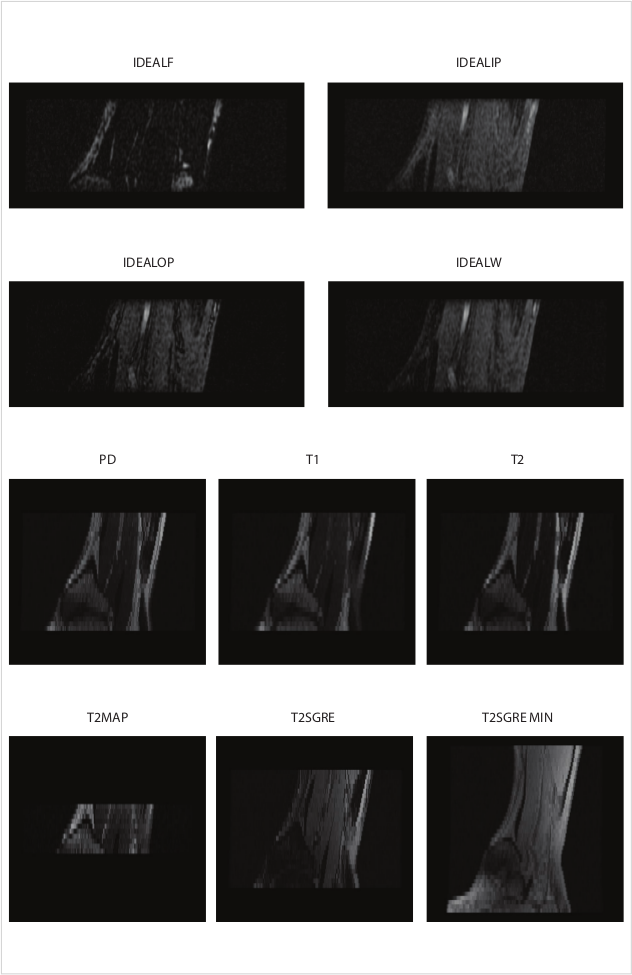
\includegraphics[width=1\textwidth]{figures/sciegno.png}
	\caption{Porównanie sekwencji RM w płaszczyźnie strzałkowej z widoczną strukturą ścięgna Achillesa.}
	\label{sagittalAchillesComp}
\end{figure}

Ograniczenia związane ze stosowaniem RM wynikają głównie z oddziaływania silnego pola magnetycznego na przedmioty z nim reagujące np. ferromagnetyki przykładowo zawarte w odłamkach metalowych; urządzenia elektryczne typu wszczepiony stymulator serca lub duże kawałki metalu jak endoprotezy, które mogą się rozgrzać na skutek indukowanych prądów. Wrażliwość pacjenta na hałas lub skłonności klaustrofobiczne również są wskazaniami do wykluczenia z badania. Ponadto urządzenie do rezonansu magnetycznego jest bardzo drogie, nieprzenośne i wymagające specjalnego otoczenia pracy. W celu wyeliminowania tych ograniczeń można posłużyć się inną metodą obrazowania medycznego opisaną w kolejnej sekcji. 

\section{Wykorzystanie ultrasonografii}
\label{USG}

Kolejną z metod obrazowania medycznego jest \textit{Ultrasonografia}, w skr. \textit{USG} (ang. \textit{Ultrasonography}, \textit{US}). Bazuje ona na efektach związanych z propagacją w tkankach \textit{ultradźwięków} tj. fal akustycznych o częstotliwościach powyżej 20 kHz. W praktyce, z uwagi na parametry związane z rozdzielczością obrazu, są to fale o częstotliwości rzędu kilku MHz, w szczególnych przypadkach kilkudziesięciu.

Propagacja fal akustycznych w przyrodzie była tematem rozważań myślicieli takich jak Pitagoras, Arystoteles czy Galileusz, którzy ugruntowali pole badań pod kolejne osiągnięcia matematyczno-inżynieryjne. W tej kwestii, do jednego z przełomów doszło w 1822 roku, kiedy to szwajcarski inżynier Daniel Colladen oraz matematyk Charles-Francois Sturm wyznaczyli przybliżoną prędkość rozchodzenia się fali akustycznej w wodzie. Badanie wykonano na Jeziorze Genewskim symultanicznie mierząc czas jaki potrzebny był dźwiękowi podwodnego wystrzału i sygnałowi dzwonka rozchodzącego się w powietrzu do przebycia drogi pomiędzy dwoma łódkami oddalonymi o 10 mil. Wyliczona wartość wyniosła wówczas 1435 m/s nie różniąc się znacząco od dzisiaj przyjmowanej estymacji równej 1480 m/s. Analogicznie, stosując nowoczesne techniki, wyliczane są obecnie prędkości rozchodzenia się fali \linebreak w innych ośrodkach takich jak powietrze, tkanki miękkie, kości itp.

58 lat po eksperymencie na Jeziorze Genewskim, w 1880 roku bracia Curie opisali w \cite{Curie1880} \textit{efekt piezoelektryczny}, czyli zjawisko polegające na pojawieniu się ładunku elektrycznego pod wpływem naprężeń mechanicznych w krysztale o anizotropowej budowie, takiej jak ma np. kwarc. W przypadku odwrotnym, przyłożenie napięcia do odpowiedniego kryształu generuje drgania (tzw. \textit{odwrotny efekt piezoelektryczny}). 

Efekty te są wykorzystywane w \textit{głowicy aparatu usg}, przyrządu do generowania \linebreak i odbierania ultradźwięków. Przykładowo, polaryzowanie kryształu piezoelektrycznego krótkim impulsem elektrycznym $\sigma_1(t)$ pobudza go do drgań na własnej \textit{częstotliwości rezonansowej}. Zakładając, że ów kryształ ma kształt walca o grubości $d$=0,64 mm, to będzie stanowił rezonator półfalowy, w którym wystąpi drganie rezonansowe o długości fali $\lambda = 2d$ czyli $\lambda = 1,28$ mm. Jeżeli wykonany jest z tytanianu baru, dla którego prędkość propagacji drgań wynosi $c$=4460 m/s, to częstotliwość drgań własnych tego kryształu wyniesie:
\begin{equation}
f = \frac{c}{\lambda} = \frac{4460 m/s}{1,28 mm} = 3,5 \; MHz.
\end{equation}
Odwrotnie, powracająca fala tzw. \textit{echo} wygeneruje impuls elektryczny $\sigma_2(t)$ wskutek drgań wywołanych w krysztale. Echo jest falą różniącą się od sygnału nadawanego, a zmiany te są w przeważającym stopniu efektem zjawisk takich jak: \textit{odbicia}, \textit{załamania}, \textit{dyfrakcja}, \textit{rozpraszanie} i \textit{pochłanianie} (zob. \cite{makarewicz1978}).

Zjawiska te zależą od częstotliwości fali, która propaguje się w ośrodku o pewnej \textit{impedancji akustycznej ośrodka} $Z$ wyrażanej jako:
\begin{equation}
Z = \rho c = \sqrt{\epsilon \rho},
\end{equation}
gdzie $c$, to prędkość rozchodzenia się fali, $\rho$ to gęstość ośrodka, a $\epsilon$ to \textit{moduł odkształcalności objętościowej}, tj. parametr opisujący jak zmieni się objętość ośrodka pod danym ciśnieniem. Parametry wybranych ośrodków zestawiono w Tabeli \ref{tab:USG-params}.
\vspace{10px} 
\renewcommand{\arraystretch}{1.2}
\begin{table}[h!]
	\setlength{\tabcolsep}{14pt}
	\centering
	\caption{Parametry ośrodków często mierzonych w badaniach USG.}
	\scriptsize
	\label{tab:USG-params}
	\begin{tabular}{l | l | l | l | l }
		%\hline
		Ośrodek  & Moduł sprężystości  & Gęstość  & Prędkość  & Impedancja akustyczna  \\  
		& [kg/m/s$^2\times10^{-8}$] & [kg/m$^3$] & [m/s] & [kg/m$^2$/s$^2\times10^{-8}$] \\ \hline \hline
		Powietrze   & 0,0000134 & 1,2 & 330 & 0,0004 \\ \hline
		Woda (20$^\circ$ C) & 2,19 & 1000 & 1480 & 1,48  \\ \hline
		Tkanki miękkie & 2,51 & 1060 & 1540 & 1,63  \\ \hline
		Tkanka tłuszczowa & 2,0 & 952 & 1450 & 1,38  \\ \hline
		Wątroba & 2,54 & 1060 & 1550 & 1,64  \\ \hline
		Mięśnie wzdłużne & 2,74 & 1080 & 1592 & 1,70  \\ \hline
		Mięśnie poprzecz. & 2,80 & 1080 & 1610 & 1,74  \\ \hline
		Mózg & 2,40 & 994 & 1550 & 1,55  \\ \hline
		Śledziona & 2,59 & 1045 & 1578 & 1,64  \\ \hline
		Krew & 2,47 & 1057 & 1057 & 1,62  \\ \hline
		Kość & 32,0 & 1912 & 4080 & 7,8  \\ \hline
		Płuca & 0,169 & 400 & 650 & 0,26  \\ \hline
	\end{tabular}
\end{table}
\renewcommand{\arraystretch}{1}

Dla przykładu, do zjawiska załamania lub odbicia dochodzi kiedy fala pada \linebreak na granicę dwóch ośrodków o różnych impedancjach akustycznych $Z_1$ i $Z_2$. Dla fali prostopadłej zależność ta opisana jest następująco:
\begin{equation}
R = \frac{I_r}{I_0} = \left(\frac{Z_1-Z_2}{Z_1+Z_2}\right)^2,
\end{equation}
gdzie $I_r$ to natężenie fali padającej, a $I_0$ odbitej. Natomiast $R$, czyli energetyczny współczynnik odbicia, jest parametrem, który rośnie wraz ze wzrostem kąta odchylenia od kierunku prostopadłego, aż do całkowitego odbicia.

Z kolei do rozpraszania bądź pochłaniania fali dochodzi kiedy to fala pokonuje daną drogę w ośrodku o pewnej $Z$, co zapisywane jest następująco:
\begin{equation}
I=I_0 \epsilon^{-\gamma x},
\end{equation}
gdzie $\gamma$ to współczynnik osłabienia zależny od $Z$, a $x$ to droga przebyta przez falę. Efekt ten można korygować poprzez dobór odpowiedniego $I_0$ lub mierząc czas powrotu i na tej podstawie wyliczając spodziewane osłabienie. Zabieg ten pozwala obrazować jednocześnie struktury położone na rożnych głębokościach.

Analiza amplitudy i częstotliwości sygnału nadanego i echa umożliwia rekonstrukcję obrazu USG. W przypadku najczęściej stosowanych w praktyce rekonstrukcji przekrojów dwuwymiarowych (tzw. \textit{tryb B}) współczesny tor budowania prezentacji wizualnej (tzw. \textit{beamforming}) wygląda następująco: 
\begin{enumerate}[noitemsep,nolistsep]
	\item Głowica ultradźwiękowa emituje impulsy w postaci wąskiej wiązki w ściśle określonym kierunku. Wiązka jest efektem interferencji sygnału z $N$ przetworników zawierających kryształy piezoelektryczne.
	\item Echa z danego kierunku pozwalają na obliczenie pojedynczego promienia akustycznego, który jest ilorazem charakterystyk nadawanego i odbieranego sygnału.
	\item Wszystkie promienie, których we współczesnych aparatach może być do kilkuset (zob. \cite{GEVoluson}), służą do formowania obrazu, który tworzony jest we \textit{współrzędnych biegunowych} ($r$, $\theta$) w przypadku głowic mechanicznych sektorowych, wieloelementowych convex czy fazowych lub we współrzędnych prostokątnych ($x$, $y$) w przypadku głowic mechanicznych lub wieloelementowych liniowych. 
\end{enumerate}

Tryb B umożliwia również wizualizację obrazów dynamicznych. Przykładowo, jeżeli na obraz składa się 400 promieni i każdy odsłuchiwany jest do głębokości 15 cm, to czas gromadzenia danych dla ośrodka o średnim c=1500 m/s wynosi $2\frac{2\times15}{1500 m/s}\times400 = 0,08$ s, czyli 12 obrazów na sekundę. Częstotliwość tę można zwiększać zmniejszając liczbę promieni lub głębokość obserwacji.

Innym często stosowanym trybem rekonstrukcji obrazu jest \textit{tryb D} bazujący \linebreak na \textit{efekcie Dopplera}, do którego dochodzi w przypadku odbicia fali od ośrodka przesuwającego się względem głowicy. Zmienia się wówczas częstotliwość fali, co wyrażone jest następującym wzorem:
\begin{equation}
f_r = 2 f_o\frac{v}{c}\cos(\theta),
\end{equation} 
gdzie $f_0$ to częstotliwość fali nadawanej.  $f_r$ to różnica pomiędzy częstotliwością odbieraną i emitowaną przez głowicę USG. Kąt $\theta$ jest kątem pomiędzy kierunkiem propagacji fali ultradźwiękowej i kierunkiem prędkości poruszającego się ośrodka. $v$ i $c$ natomiast to odpowiednio prędkości ośrodka i dźwięku w ośrodku.

Dla przykładu, im większa prędkość komórek przesuwających się w monitorowanym ciele pacjenta, tym większa jest $f_r$. Dlatego tryb D z powodzeniem jest wykorzystywany np. do monitorowania przepływu krwi w dużych naczyniach takich jak tętnice.

Rozwinięciem trybu D jest tryb \textit{Power D} (od ang. \textit{Power Doppler}). W tym trybie zamiast przesunięcia częstotliwości interpretowana jest moc sygnału dopplerowskiego. Za pomocą odpowiedniego parametru nazywanego \textit{gain} można wzmacniać sygnał Power D uwidaczniając np. informacje pochodzące od przepływów krwi z niewielką prędkością w charakteryzujących się małą średnicą naczyniach krwionośnych. Jest to również możliwe, gdyż tryb Power D ma nawet trzykrotnie większą czułość niż standardowy tryb D \cite{Babcock1996}. Wynika to z faktu, że Power D nie uwzględnia informacji o prędkości czy kierunku przepływów, a jest sumą wszystkich możliwych przesunięć częstotliwości w zadanym fragmencie obrazowanego obiektu.

W kontekście ścięgna Achillesa tryb Power D może służyć do oceny unaczynienia ścięgna w kolejnych etapach gojenia, które jak wiadomo z p. \ref{gojenie} zmienia się w czasie. Tryb B natomiast może być użyteczny do obrazowania struktury tkanek miękkich. W praktyce wykorzystywana jest zwłaszcza możliwość zobrazowania ukierunkowania struktur włókien ścięgnistych na podstawie czego radiolog może wnioskować o fazie gojenia. Składowa czasowa jest interesująca z perspektywy badań funkcjonalnych i m.in. fizjoterapeuty oceniającego ślizg w ścięgnie przy wykonywaniu odpowiednich ruchów np. zginania podeszwowo-grzbietowego stopy. 

\begin{figure}[h!]
	\centering
	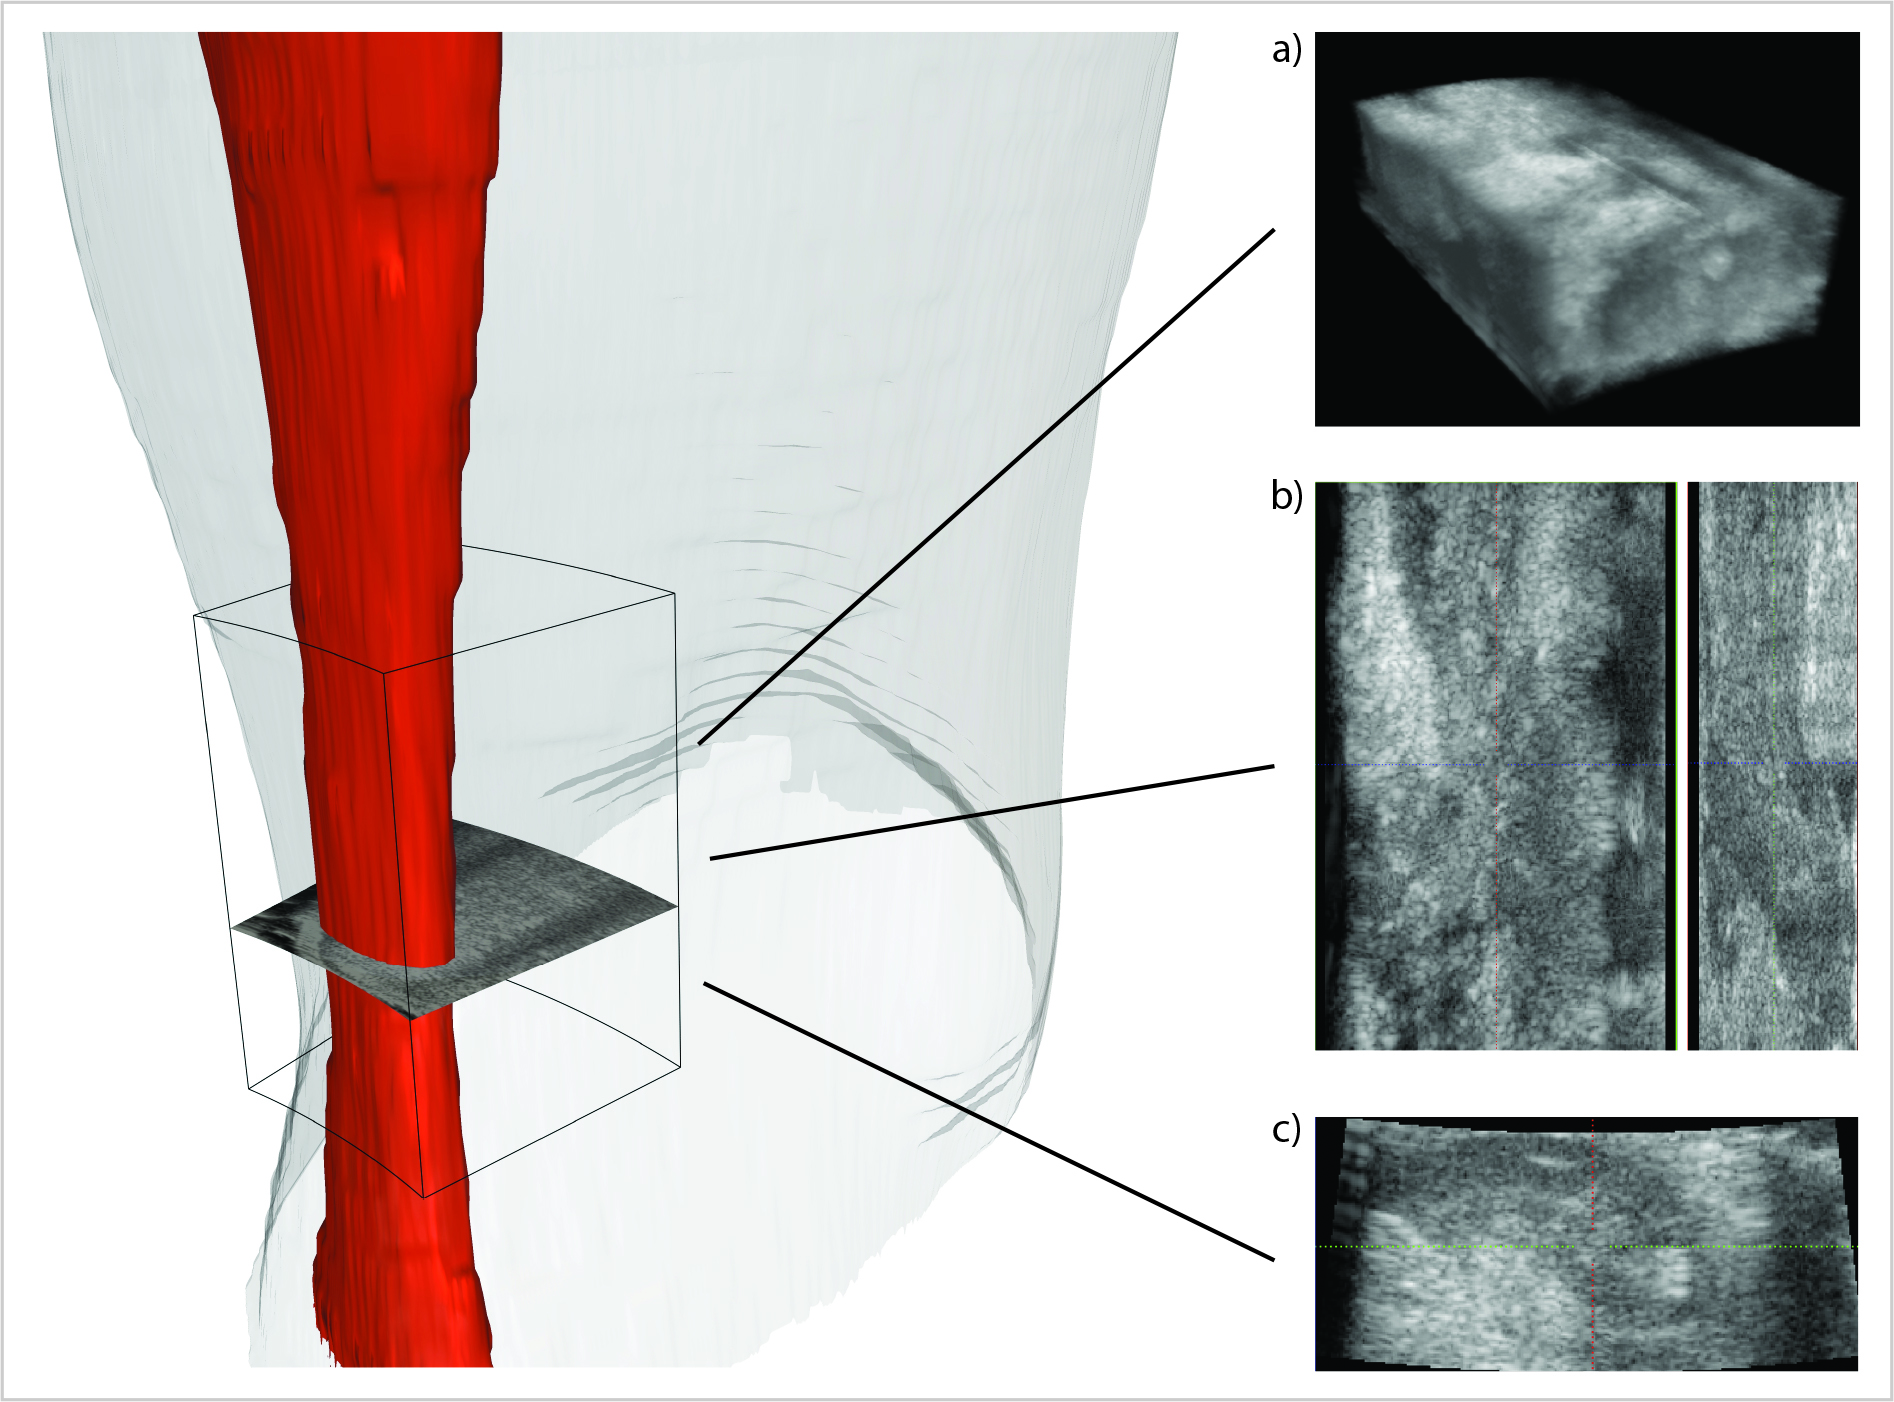
\includegraphics[width=1\textwidth]{figures/sciegnoUSG.jpg}
	\caption{Obszar obrazowania ścięgna Achillesa w USG, wraz z danymi wolumetrycznymi -- a), danymi w przekrojach strzałkowym i czołowym -- b) oraz danymi w przekroju poprzecznym -- c).}
	\label{sagittalAchillesComp}
\end{figure}


W porównaniu do rezonansu magnetycznego obszar pojedynczego obrazowania jest mniejszy. W kwestii ograniczeń należy również zwrócić uwagę na fakt, że fale akustyczne używane w USG nie propagują się dobrze przez kości i gazy. Zastosowanie do oceny struktur umiejscowionych w otoczeniu lub składających się w większości z takich ośrodków (jak np. mózg lub płuca) znajduje zatem RM. Rezonans Magnetyczny umożliwia również uzyskanie obrazów o lepszej jakości detali. Sam czas badania jest natomiast dłuższy i w większości przypadków niemożliwe jest obrazowanie w czasie rzeczywistym, co z kolei jest naturalne dla techniki USG.

W wymiarze finansowym istotny jest fakt, że aparat do USG kosztuje średnio 10 razy mniej niż aparatura RM. Jak jednak wspomniano, z uwagi na jakość detali, uzyskiwane obrazy są trudniejsze do interpretacji, stąd trudności w  wyszkoleniu kadry. 

Nowe rozwiązania mogą wpłynąć na znaczące zmiany w USG zarówno w warstwie sprzętowej jak i oprogramowania. Po pierwsze postępuje zmiana technologiczna, a przetworniki z piezoelektrykami zastępowane są przetwornikami budowanymi \linebreak w technologi MEMS np. cMUT, czy pMUT (zob. \cite{Butterfly2018})  pozwalające m.in. przetwarzać surowy sygnał ultradźwiękowy (zob. \cite{US4US}). Wynika to z faktu, że dzięki przetwornikom MEMS można wytworzyć cały układ generujący drgania w krzemie w jednym procesie technologicznym razem z dedykowanym układem do zadanej aplikacji (ang. \textit{Application-Specific Integrated Circuit} w skr. \textit{ASIC}). Takie podejście znacząco redukuje koszty oraz implikuje możliwość miniaturyzacji urządzeń.

W warstwie oprogramowania do USG należy zwrócić uwagę na rozwój algorytmów sztucznej inteligencji pozwalających wydobyć i zinterpretować interesującą informację z niskiej jakości obrazów. Przykładowo w \cite{Cunningham2017} algorytmy sztucznej inteligencji zostały użyte do określenia orientacji włókien mięśniowych, a w \cite{NVIDIA-CLARA} \linebreak do segmentacji komór serca w czasie rzeczywistym. 

Obiecujący jest też rozwój metod \textit{UTC} (od ang. Ultrasonography Tissue Characterization). W 2003 r., w \cite{Bakker2003} Bakker et. al. przedstawili pracę pokazującą w jakim stopniu obraz USG jest mieszanką echa związanego z budową tkanki, a w jakim z \textit{interferencji}, czyli nakładania się fal. W zależności od stabilności echa można zatem wnioskować czy obserwowana struktura składa się głównie z dużych, stałych struktur wywołujących stabilne echo, czy np. płynów lub małych włókienek powodujących zmienne interferencje. Jako referencji dla studiowanego echa używa się badań histologicznych (zob. \cite{Bakker2000}). Na tej podstawie sklasyfikowano 4 różne rodzaje echa i jak zasygnalizowano w pracach \cite{vanSchie2009} i \cite{Heyward2018} informacja o proporcjach występowania tych rodzai echa może być użyta do oceny struktury ścięgna Achillesa. Metoda ta nie została jednak jeszcze w pełni zwalidowana i możliwości wnioskowania na jej podstawie \linebreak są wciąż niejasne (zob. \cite{Heyward2018}).

USG i inne techniki obrazowania medycznego nie są jedynymi metodami oceny gojenia się ścięgna Achillesa. W kolejnej sekcji zostały opisane techniki oceny funkcji ścięgna, które samodzielnie jak i w połączeniu z analizą obrazową stanowią wartościową informację diagnostyczną.

\section{Wykorzystanie badań biomechanicznych}
\label{biomechanika}
W poprzednich sekcjach zostały opisane dwie najczęściej wykorzystywane obrazowe metody monitorowania procesu gojenia się ścięgna Achillesa. Komplementarnie, podczas rehabilitacji może być również wykonana \textit{ocena funkcjonalna}, technika weryfikująca w jakim stopniu dany element (tkanka, narząd, organizm) może realizować swoje zadania. W przypadku monitorowania gojenia się ścięgna Achillesa najczęściej w tym celu stosuje się \textit{ocenę biomechaniki}, czyli badania pozwalające wnioskować na temat właściwości mechanicznych elementów składowych organizmów żywych. 

Najbardziej zaawansowane i dokładne metody oceny biomechaniki stosowane współcześnie możliwe są do wykonania przy użyciu urządzeń pomiarowych takich jak:
\begin{itemize}[noitemsep,nolistsep]
	\item \textit{Komputerowa analiza ruchu} (ang. \textit{Motion Capture}) -- narzędzie wykorzystujące systemy czujników do zapisu informacji o zmianach położenia obiektu rejestrowanego np. pacjenta. Do wiodących rozwiązań należy zaliczyć systemy firm Vicon \cite{Vicon}, czy BTS \cite{BTS}.
	\item \textit{Płyty dynamometryczne} (ang. \textit{Force Plates}) -- narzędzie wykorzystywane \linebreak do pomiaru sił reakcji podłoża w trzech prostopadłych płaszczyznach. Dzięki temu można określić sumaryczny udział mięśni w generowaniu sił odpowiadających za balans ciała, ruch w danym kierunku oraz przeciwstawianie się sile grawitacji. Do wiodących rozwiązań należą płyty firmy Kistler \cite{KISTLER}.
	\item \textit{Elektromiografia}, w skr. \textit{EMG} (ang. \textit{Electromyography}) -- narzędzie do pomiaru pobudzeń poszczególnych grup mięśniowych podczas ruchu. Wykorzystywane jest m.in. do określenia rozkładu sił zmierzonych przez płyty dynamometryczne na poszczególne mięśnie.
\end{itemize}

Synchronizacja danych z powyższych urządzeń umożliwia konstrukcję modeli układu mięśniowo-szkieletowego i symulacje funkcji poszczególnych grup mięśniowych oraz ścięgien w zadanych problemach.

Danymi stosowanymi do uszczegółowienia takich modeli są np.: wymiary poszczególnych segmentów ciała (goleń, udo, tors) tzw. pomiary antropometryczne; maksymalne siły izometryczne mierzone z użyciem systemów takich jak Biodex; geometria kości mierzonych np. z pomocą tomografii komputerowej ew. RM; lokalizacja przyczepów mięśniowych określanych przy pomocy RM lub USG; środki masy poszczególnych segmentów określanych np. przy użyciu badania \textit{DXA} (od ang. \textit{Double X Ray Absorption}) lub tomografii komputerowej; charakterystykę włókien mięśniowych widocznych w USG.

Z uwagi na dużą liczbę możliwych do zmierzenia parametrów, ich integracja odbywa się w modelach komputerowych zaimplementowanych w różnego rodzaju oprogramowaniu do symulacji biomechanicznych. Do najczęściej używanych modeli należą opisane w \cite{John2013} Gait 2392 i 2354 oraz obecnie najbardziej złożony -- \textit{AnyBody Full Body Model} \cite{Bassani2017}. 

Historia komputerowo wspomaganego, kompleksowego modelowania biomechaniki ruchu sięga wczesnych lat 90-tych ubiegłego wieku, kiedy to Delp i Loan przedstawili oprogramowanie SIMM \cite{Delp1990}. Obecnie SIMM jak również inne oprogramowania komercyjne takie jak: Visual 3D (Cmotion Inc.) \cite{Visual3D}, Anybody (Anybody Technology) \cite{AnyBody}, czy Adams (MSC Software Corp.) \cite{Adams}, dostarczają narzędzi \linebreak do wartościowych symulacji np. chodu \cite{Steele2010}, biegu \cite{Hamner2010} jak również konsekwencji różnych zabiegów chirurgicznych \cite{Gomes2013} i chorób \cite{Shao2009}. Istnieją również narzędzia otwarte, do których należą szeroko wykorzystywany OpenSim \cite{Delp2007} rozwijany na Uniwersytecie Stanforda, czy też Human Motion \cite{Riken} wywodzący się z instytutu badawczego RIKEN w Japonii.

Powyżej przedstawione kompleksowe badania w praktyce realizowane są rzadko z uwagi na ich wysokie koszty. Dla przykładu w Polsce, ośrodki wyposażone \linebreak w sprzęt pomiarowy takiej klasy to np. Instytut "Pomnik – Centrum Zdrowia Dziecka", Warszawski Uniwersytet Medyczny, Akademia Wychowania Fizycznego imienia Józefa Piłsudskiego, czy komercyjna placówka Fizjofit w Gliwicach. W celu obniżenia kosztów badania stosuje się wybiórcze podejście i selekcję parametrów pomiarowych uznanych przez ekspertów dziedzinowych za wystarczające do analizy zadanego problemu. Dla przykładu, badania stosowane do oceny biomechaniki ścięgna Achillesa w placówce Carolina Medical Center (gdzie zrealizowane były badania wykorzystywane w tej pracy) składają się z następujących pomiarów (zob. \cite{CMC}):

\begin{enumerate}[noitemsep,nolistsep]
	\item Pomiar \textit{ATRS} (od ang. \textit{Achilles Tendon Total Rupture Score}) -- oceniany \linebreak w skali od 0 do 100 \cite{NilssonHelander2007} poziom ograniczenia, z którymi pacjenci borykają się w następstwie urazu.
	\item Pomiar stabilograficzny na platformie dynamometrycznej -- mierzone są wychylenia środka ciężkości. Pacjent ma za zadanie utrzymanie równowagi \linebreak na niestabilnym podłożu. Wykonane są dwie próby po 30 sekund kolejno na prawej i lewej kończynie dolnej na dynamicznej platformie dynamometrycznej Biodex Balance System. Wyniki obu prób są porównane między sobą. 
	\item Pomiar stabilograficzny na platformie statycznej -- mierzona jest droga wychylenia środka masy pacjenta w trakcie stania jednonóż na platformie dynamometrycznej, statycznej.
	\item Pomiar sił reakcji na ścieżce podometrycznej -- mierzony jest rozkład sił nacisków podeszwowej strony stóp na podłoże (jedynie w kierunku prostopadłym do podłoża). Pomiar wykonywany jest podczas stania swobodnego, wspięć \linebreak na palce oraz przysiadu bez odrywania pięt. Dokonywana jest również analiza chodu (3 przejścia) i biegu (5 przebiegnięć). Na podstawie sił reakcji wyliczane są parametry: rotacja podudzia [$^\circ$], długość kroków [cm], udział fazy podparcia [\%], udział fazy przenoszenia [\%], maksymalna siła na pięcie [N] oraz maksymalna siła na palcach [N].
	\item Pomiar skoczności i mocy (tzw. siły dynamicznej) kończyn dolnych -- mierzona jest moc maksymalna $P_{max}$ i średnia $P_m$, maksymalna wysokość uniesienia $h_{max}$ i obniżenia $k$ środka masy ciała przed odbiciem. Wykonywane są wyskoki pionowe z miejsca na platformie dynamometrycznej. Realizowane są dwie próby obunóż oraz na prawej i lewej kończynie dolnej. W celu pełnego zaangażowania kończyn dolnych pacjent podczas badania trzyma ręce na biodrach. 
	\item Pomiary momentów sił mięśni stawu skokowego -- mierzone są maksymalne wartości momentu siły mięśni zginaczy podeszwowych i grzbietowych stawu skokowego [Nm] oraz deficyt pomiędzy operowaną i zdrową kończyną dolną [\%]. Momenty sił mierzone są w dwóch pozycjach tj. z wyprostowanym oraz zgiętym do 50 stopni stawem kolanowym \cite{Orishimo2008}. Pomiar realizowany jest w warunkach izometrii i izokinetyki w trzech prędkościach kątowych 60$^\circ$/s (5 powtórzeń), 120$^\circ$/s (8 powtórzeń) oraz 180$^\circ$/s (10 powtórzeń) przy wykorzystaniu urządzenia Humac Norm (USA). Przed badaniem pacjent odbywa 5 minutową rozgrzewkę na steperze.
\end{enumerate}

Wymienione badania zostały określone przez ortopedów i fizjoterapeutów jako wystarczające do oceny przywracania funkcji ścięgna Achillesa po rekonstrukcji. 

Wraz z oceną strukturalną realizowaną poprzez badania obrazowe i wiedzą ekspercką, informacja tak zgromadzona może służyć do subiektywnego monitorowania procesu gojenia się ścięgna. Do skutecznej obiektywizacji tego procesu potrzebne są jednak dodatkowe metody bazujące na agregacji ilościowych współczynników \linebreak i automatycznym wnioskowaniu na ich podstawie. Do tej grupy należą algorytmy sztucznej inteligencji opisane dalej w pracy. 
\chapter{Konwolucyjne sieci neuronowe}
\label{CNNs}
\textit{Konwolucyjne sieci neuronowe} (ang. \textit{Convolutional Neural Networks}, CNN) są biologicznie inspirowanymi sztucznymi sieciami neuronowymi. Należą do zbioru \textit{głębokich sieci neuronowych} (ang. \textit{Deep Neural Networks}, DNN), które z kolei są podzbiorem \textit{systemów uczących się} (ang. \textit{Machine Learning Systems}) tj. algorytmów nie wymagających explicite programowania do ustalenia swoich parametrów. Algorytmy te często określane są obecnie wspomnianym we wstępie tej rozprawy terminem Wąskiej Sztucznej Inteligencji.

Pierwsze matematyczne formalizmy dotyczące CNN zostały zaproponowane już w latach 40-tych XX wieku, natomiast fundamentalne inspiracje biologiczne dały badania nad korą wzrokową kotów Hubel'a i Wiesel’a z lat 50-tych i 60-tych (zob. \cite{Wurtz2009}). M.in. dzięki pracom tych neurofizjologów ustalono, że kora wzrokowa zawiera złożone układy komórek, które odpowiadają za przetwarzanie informacji z wybranych regionów pola widzenia, sumarycznie pokrywając je w całości. Komórki kory wzrokowej działają zatem jak lokalne filtry przestrzeni wejściowej zaprojektowane tak, aby wydobyć istotne informacje z naturalnych obrazów. Dla przykładu reagują one na orientację linii, kształty i kolory.

W odróżnieniu od naturalnych struktur biologicznych sieci konwolucyjne operują przeważnie na reprezentacji cyfrowej obrazu. Zapisywana jest ona w postaci tablicy liczb tzw. \textit{macierzy} o współrzędnych ($x$, $y$), gdzie $x$ to kolumna macierzy, a $y$ wiersz. W przypadku obrazów trójwymiarowych dochodzi jeszcze trzecia składowa, a zamiast macierzy użyta jest wówczas ogólna postać odwzorowania wieloliniowego, czyli \textit{tensor}.

W obrazach cyfrowych dla każdego punktu ($x$, $y$), tzw. \textit{piksela}, kodowana jest informacja o wartości funkcji obrazowej $I$($x$, $y$). Na tej podstawie dzielimy obrazy na:
\begin{itemize}
	\item binarne – gdzie kodowane są jedynie dwie możliwe wartości $I$ (0 lub 1);
	\item monochromatyczne – gdzie kodowana jest informacja o natężeniu jednej barwy (najczęściej są to odcienie szarości lub brązu tzw. \textit{sepia});
	\item kolorowe – gdzie kodowane są wartości natężenia składowych koloru.
\end{itemize}
Do zakodowania informacji o wartości funkcji $I$ w obrazie binarnym potrzebny jest jeden bit na punkt. Odcienie obrazu monochromatycznego lub pojedyncze składowe punktu obrazu kolorowego kodowane są przy pomocy 8--16 bitów, co uzależnione jest od zakresu wartości występujących w danych lub precyzji wymaganej do obliczeń. Przykładowo, obrazy medyczne przetwarzane w tej pracy należą do grupy obrazów monochromatycznych i są zapisywane w reprezentacji 16 bitowej z uwagi na zakres wartości występujących w sygnale RM.

W sieciach konwolucyjnych, procesy zachodzące w korze wzrokowej są modelowane przy użyciu odpowiednio dobranych parametrów i funkcji służących do ekstrakcji istotnych informacji obrazowych i ich przetwarzania. Parametry wykorzystywane do wstępnej ekstrakcji informacji grupowane są w \textit{filtry}, które realizują funkcję \textit{splotu} maski $K$ z kolejnymi fragmentami funkcji $I$. $K$ jest najczęściej macierzą kwadratową o wymiarze $N$, gdzie zazwyczaj $N$ = {1, 3, 5, 7, 9, 11}. Większe wymiary $K$ nie są często stosowane z uwagi na rosnącą wraz z $N$ złożonością obliczeniową. Równanie splotu dyskretnego można zapisać następująco:
\begin{equation}
	I'\left(x, y\right) = \sum_{j=-n}^{n} \sum_{i=-k}^{k} I\left(x - j, y - i \right)K\left(j, i\right),
\end{equation}
gdzie $I'$ jest nową funkcją obrazową powstałą po filtracji, a $i$ i $j$ to kolejne współrzędne maski filtru w odniesienia do jego punktu centralnego. Dla wartości brzegowych podczas realizacji splotu współrzędne poza sygnałem przyjmują z reguły wartość 0. Rzadziej stosuje się inne metody takie jak: odbicie wartości $I$ obrazu poza jego granicami; powtórzenie wartości $I$ obrazu bez odbicia; modyfikację wymiaru maski filtru na brzegu obrazu, tak by nie wychodziła poza jego granicę.

W kontekście sieci konwolucyjnych, pojedynczy splot filtru z obrazem wejściowym nazywany jest \textit{cechą} (zob. \cite{Hijazi2015}). W ostatnich latach powstało wiele algorytmów do wizualizacji cech umożliwiających wydajną analizę wyników działania sieci konwolucyjnych np.: Saliency Maps \cite{DBLP:journals/corr/SimonyanVZ13}, GradCam \cite{DBLP:journals/corr/SelvarajuDVCPB16} czy CNNVIS \cite{DBLP:journals/corr/LiuSLLZL16}. Zasada działania tych algorytmów bazuje na wstecznej propagacji informacji, co skutkuje możliwością selekcji cech, które mają zasadniczy wpływ na wynik końcowy wnioskowania. Grupy cech obliczane na tym samym obszarze obrazu wejściowego nazywane są \textit{mapami cech} (ang. \textit{feature maps}). Zazwyczaj mapy cech zawierają hierarchicznie uporządkowaną strukturę składającą się z cech od najniższego do najwyższego poziomu komplikacji (np. od charakterystycznych skupisk pikseli, przez obiekty składowe do finalnego kształtu). Do cech najniższego rzędu zaliczyć można:
\begin{itemize}
	\item \textit{krawędzie} -- ciągi punktów o gwałtownych zmianach $I$($x$, $y$);
	\item \textit{rogi} -- przecięcia dwóch krawędzi;
	\item \textit{grzbiety} lub \textit{doliny} -- odpowiednio lokalne maksimum lub minimum funkcji $I$;
	\item \textit{skupiska} (ang. \textit{blobs}) -- obszary jednorodnych wartości funkcji $I$ różniących się znacząco od najbliższego otoczenia; 
	\item \textit{tekstury} -- charakterystyczne, przestrzenne ułożenie wartości funkcji $I$ w powtarzające się wzory.
\end{itemize}

Wszystkie cechy wyższego rzędu są kombinacją wyżej wymienionych składowych podstawowych, tworzących bardziej skomplikowane struktury odpowiadające charakterystycznym obiektom znajdującym się w obrazach wejściowych. 

Na podstawie cech, na końcu toru przetwarzania danych z wykorzystaniem sieci neuronowych, realizowane jest wnioskowanie, gdzie w zależności od problemu można wyszczególnić następujące zadania:
\begin{itemize}
	\item \textit{segmentację} -- podział obrazu na spójne fragmenty, najczęściej wiążące się z wyodrębnieniem \textit{obiektu} $A_1$ z \textit{tła} $A_2$ na podstawie ustalonego progu lub miary np.:
	\begin{equation*}
	\begin{aligned}
	I(x,y) \geq T_p \Rightarrow (x,y) \in A_1 \\
	I(x,y) < T_p \Rightarrow (x,y) \in A_2,
	\end{aligned}
	\end{equation*} 
	przy czym metody ustalania wartości progowej $T_p$ lub wielu wartości {$T_p^1$,...,$T_p^n$} są obszarem szerokich badań (zob. \cite{DBLP:journals/corr/abs-1005-4020});
	\item \textit{klasyfikację} -- przyporządkowanie obiektu do odpowiedniej klasy (np. tkanka zdrowa lub patologiczna);
	\item \textit{detekcję} -- binarne rozróżnienie traktujące o tym czy obiekt znajduje się w obrazie czy nie;
	\item \textit{śledzenie} -- detekcja lub też klasyfikacja obiektów w kolejnych krokach czasowych.
\end{itemize} 

Jeszcze do niedawna tor przetwarzania danych w większości badań wykorzystujących uczenie się maszyn, operacje wyliczenia cech i wnioskowanie końcowego zawierał w dwóch osobnych krokach\footnote{Są wyjątki od tej reguły jak np. \cite{10.1007/978-3-319-58667-0_7}, inkrementalny algorytm SVM.}. Porównanie tego schematu z obecnie funkcjonującym podejściem realizowanym w algorytmach głębokiego uczenia się przedstawiono na Rys. \ref{DLworkflow}.
\begin{figure}[h!]
	\centering
	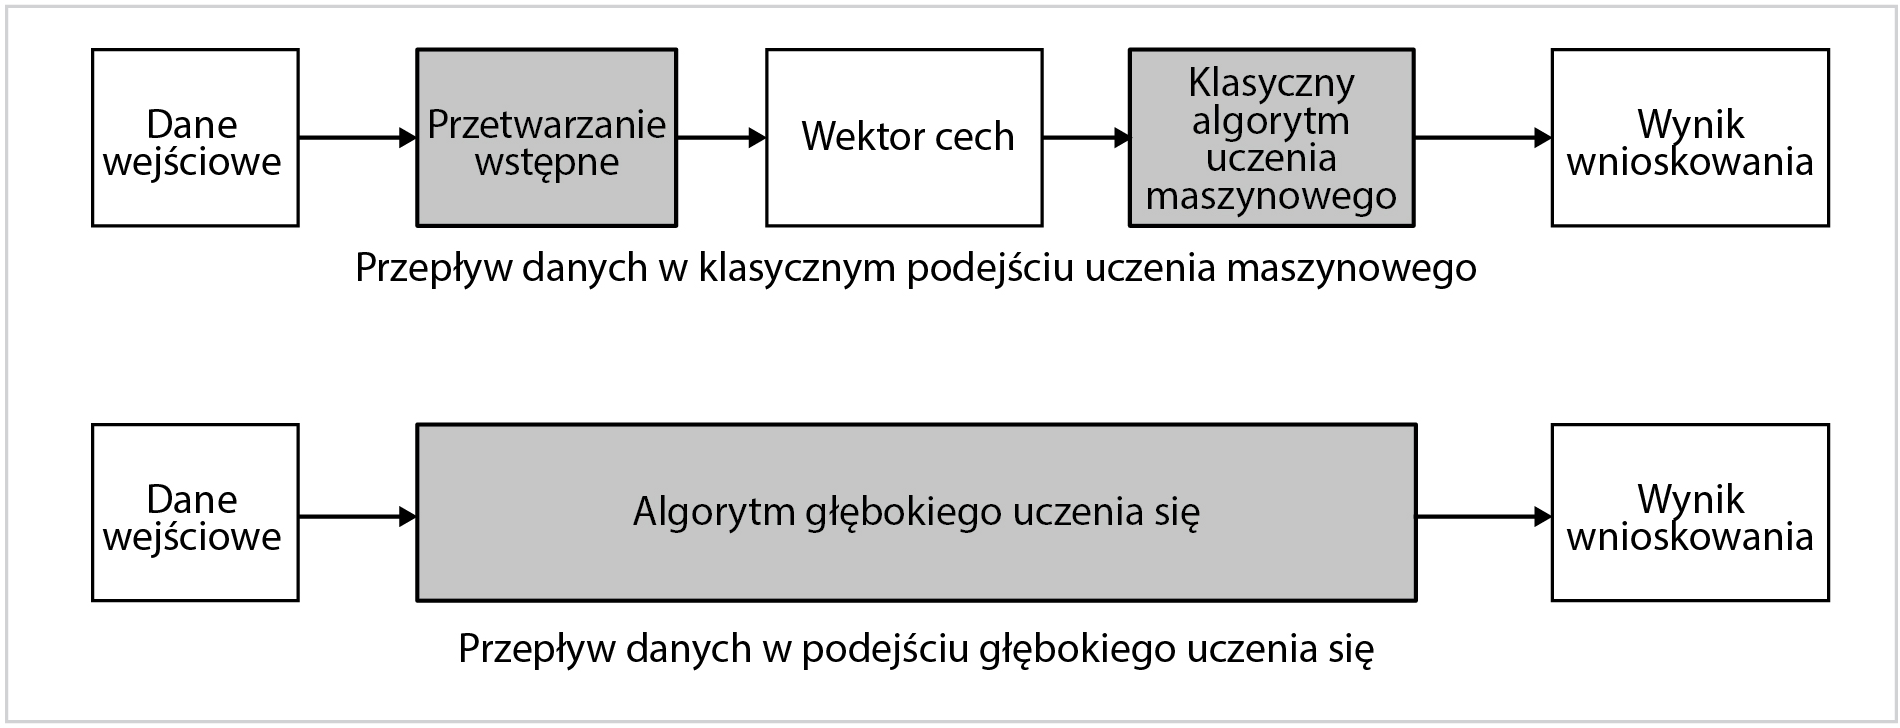
\includegraphics[width=1\textwidth]{figures/DLworkflow.png}
	\caption{Porównanie schematów przetwarzania danych z wykorzystaniem metod głębokiego uczenia się i innych algorytmów.}
	\label{DLworkflow}
\end{figure}

W nowym podejściu zarówno ekstrakcja cech jak i ostateczne wnioskowanie na ich podstawie realizowane jest w jednym kroku, co nazywane jest paradygmatem \textit{end-to-end learning}. Na przestrzeni lat wprowadzano kolejne składowe, które finalnie utworzyły obecnie funkcjonujące podejście. W kontekście poznania tych komponentów, w kolejnej sekcji omówiono dokładniej zarys historyczny przedstawiający ewolucję nowego paradygmatu. 

\section{Rys historyczny}

Pierwszy formalny model neuronu został zaproponowany przez Warrena McCulloch i Waltera Pitts w roku 1943 (zob. \cite{McCulloch1943}). Była to bramka logiczna, której wyjście stawało się aktywne w momencie, gdy liczba aktywnych wejść przekroczyła pewien zdefiniowany próg. Taka zależność sygnału wyjściowego $y$ od sygnałów wejściowych $x_1$,...,$x_n$ została potem nazwana \textit{funkcją aktywacji neuronu}, którą zapisujemy jako:
\begin{equation}
\label{eqActFunc}
y=f\left(x_1, x_2,..., x_n\right)
\end{equation}

W modelu neuronu McCulloch-Pitts można było modyfikować parametr progu, nie istniała natomiast możliwość uczenia się takiej architektury. Problem ten rozwiązano w 1957 proponując sztuczną sieć neuronową zawierającą wiele neuronów z ważonymi połączeniami między sobą (zob. \cite{Rosenblatt1957}). Sieć nazwano perceptronem, co było implikacją zamiłowania jego twórcy Franka Rosenblatta do aplikacji związanych z percepcją, zwłaszcza mowy czy pisma. Schemat sieci pokazano na Rys. \ref{Perceptron}.
\begin{figure}[h!]
	\centering
	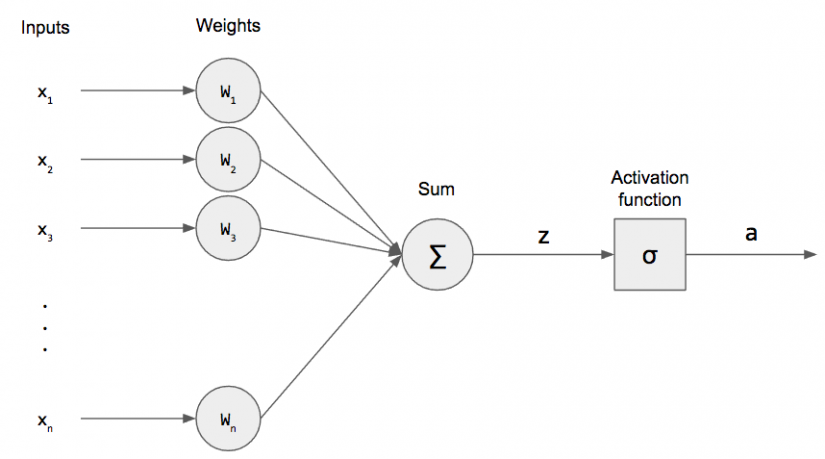
\includegraphics[width=1\textwidth]{figures/perceptron.png}
	\caption{Topologia perceptronu.}
	\label{Perceptron}
\end{figure}

Zastosowanie dodatkowej jednowymiarowej tablicy współczynników, czyli \textit{wektora wag} $w$ = ($w_1$,...,$w_n$) dało możliwość uczenia się poprzez adaptacyjną zmianę wartości poszczególnych jego elementów. W modelu Rosenblatta zastosowano ponadto progową funkcję aktywacji z progiem $T_a$:
\begin{equation}
y(z)=\begin{cases} 0, & n < T_a, \\ 1, & n \ge T_a, \end{cases}
\end{equation}
gdzie $z$ to suma ważona wyjść poszczególnych neuronów:
\begin{equation}
\label{eqLinActFunc}
z=\sum_{i=1}^{n}w_i x_i
\end{equation}

Dla przykładu, w dwuwymiarowej przestrzeni sygnałów wejściowych {$x_1$, $x_2$}  działanie perceptronu można opisać jako wyliczenie funkcji liniowej rozdzielającej obserwacje $o_1$ od $o_2$. W trzech wymiarach będzie to płaszczyzna, a w $n$-wymiarach, hiperpłaszczyzna. Z uwagi na swój liniowy charakter, perceptron proponowany przez Rosenblatta miał wiele ograniczeń, które szczegółowo sformułowali w 1969 roku Marvin Minsky i Seymour Papert w książce \textit{Perceptrons} (zob. \cite{Minsky1969}). Autorzy opublikowali listę problemów, których nie można było rozwiązać z użyciem perceptronu m.in. do najszerzej dyskutowanych należał przykład związany z brakiem możliwości modelowania \textit{funkcji XOR}, aktywującej wyjście przy aktywnym jednym z dwóch wejść.

Część z opisanych przez Minsky-Papert problemów udało się rozwiązać dzięki pracy Davida Rumelharta, Geoffa Hintona i Ronalda Williamsa, którzy opublikowali w 1986 roku pracę \cite{Rumelhart1986}, traktującą o perceptronach wielowarstwowych. Schemat takiej sieci zaprezentowano na Rys. \ref{MLperceptron}
\begin{figure}[h!]
	\centering
	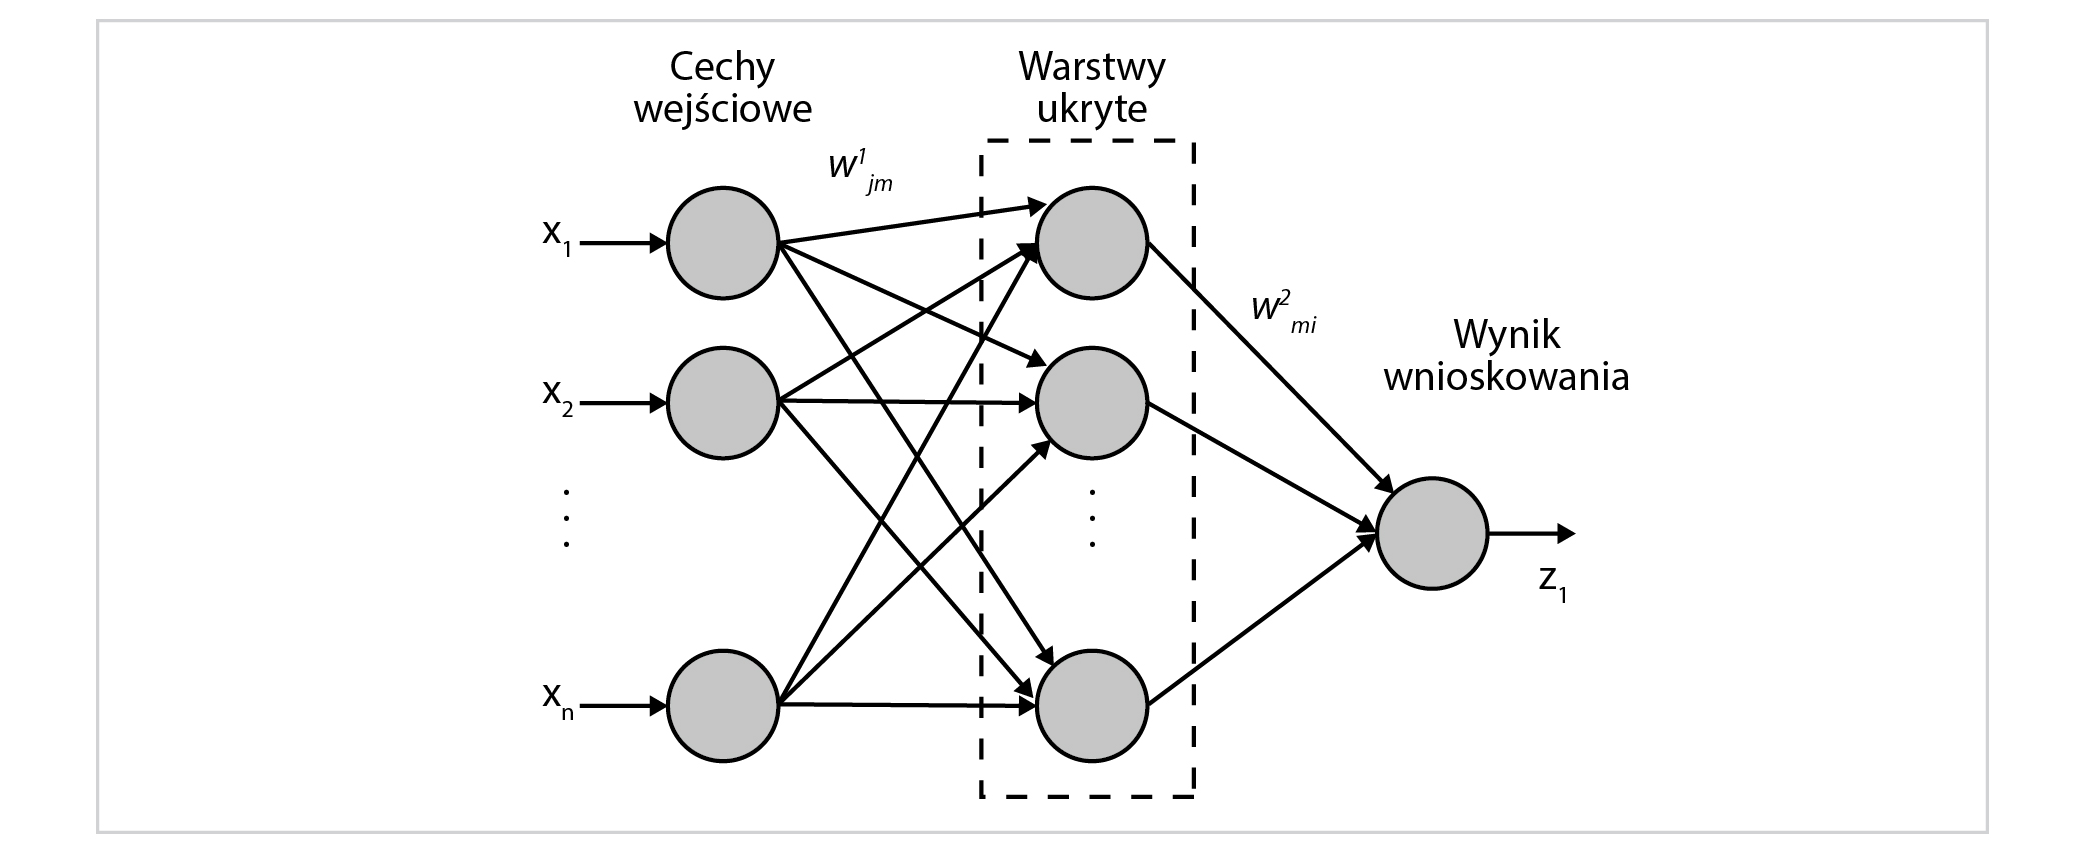
\includegraphics[width=1\textwidth]{figures/MLperceptron.png}
	\caption{Topologia perceptronu wielowarstwowego.}
	\label{MLperceptron}
\end{figure}

Spośród najważniejszych innowacji wprowadzonych w perceptronie wielowarstwowym wyszczególnić można zastosowanie w praktyce nowego algorytmu uczenia się sieci, który został opisany w kolejnej sekcji, jak również wykorzystanie nowej, sigmoidalnej funkcji aktywacji:
\begin{equation}
\label{eqSigActFunc}
y(x) = \frac{1}{1 + e^{-x}}
\end{equation}

Po wprowadzeniu innowacji możliwe stało się modelowanie funkcji XOR jak i innych problemów nieliniowych o praktycznym wymiarze. 

Kolejny przełom nastąpił w 1989 roku kiedy to Yann LeCunn, uczeń Geaoffa Hintona, zaprezentował swoje wyniki klasyfikacji odręcznego pisma z użyciem sieci wielowarstwowych (zob. \cite{NIPS1989_293}). Finalnie, badania te doprowadziły do przedstawienia w 1998 roku protoplasty współczesnych sieci konwolucyjnej -- LeNet (zob. \cite{Lecun1998}). Architekturę LeNet przedstawiono na Rys. \ref{LeNet}.
\begin{figure}[h!]
	\centering
	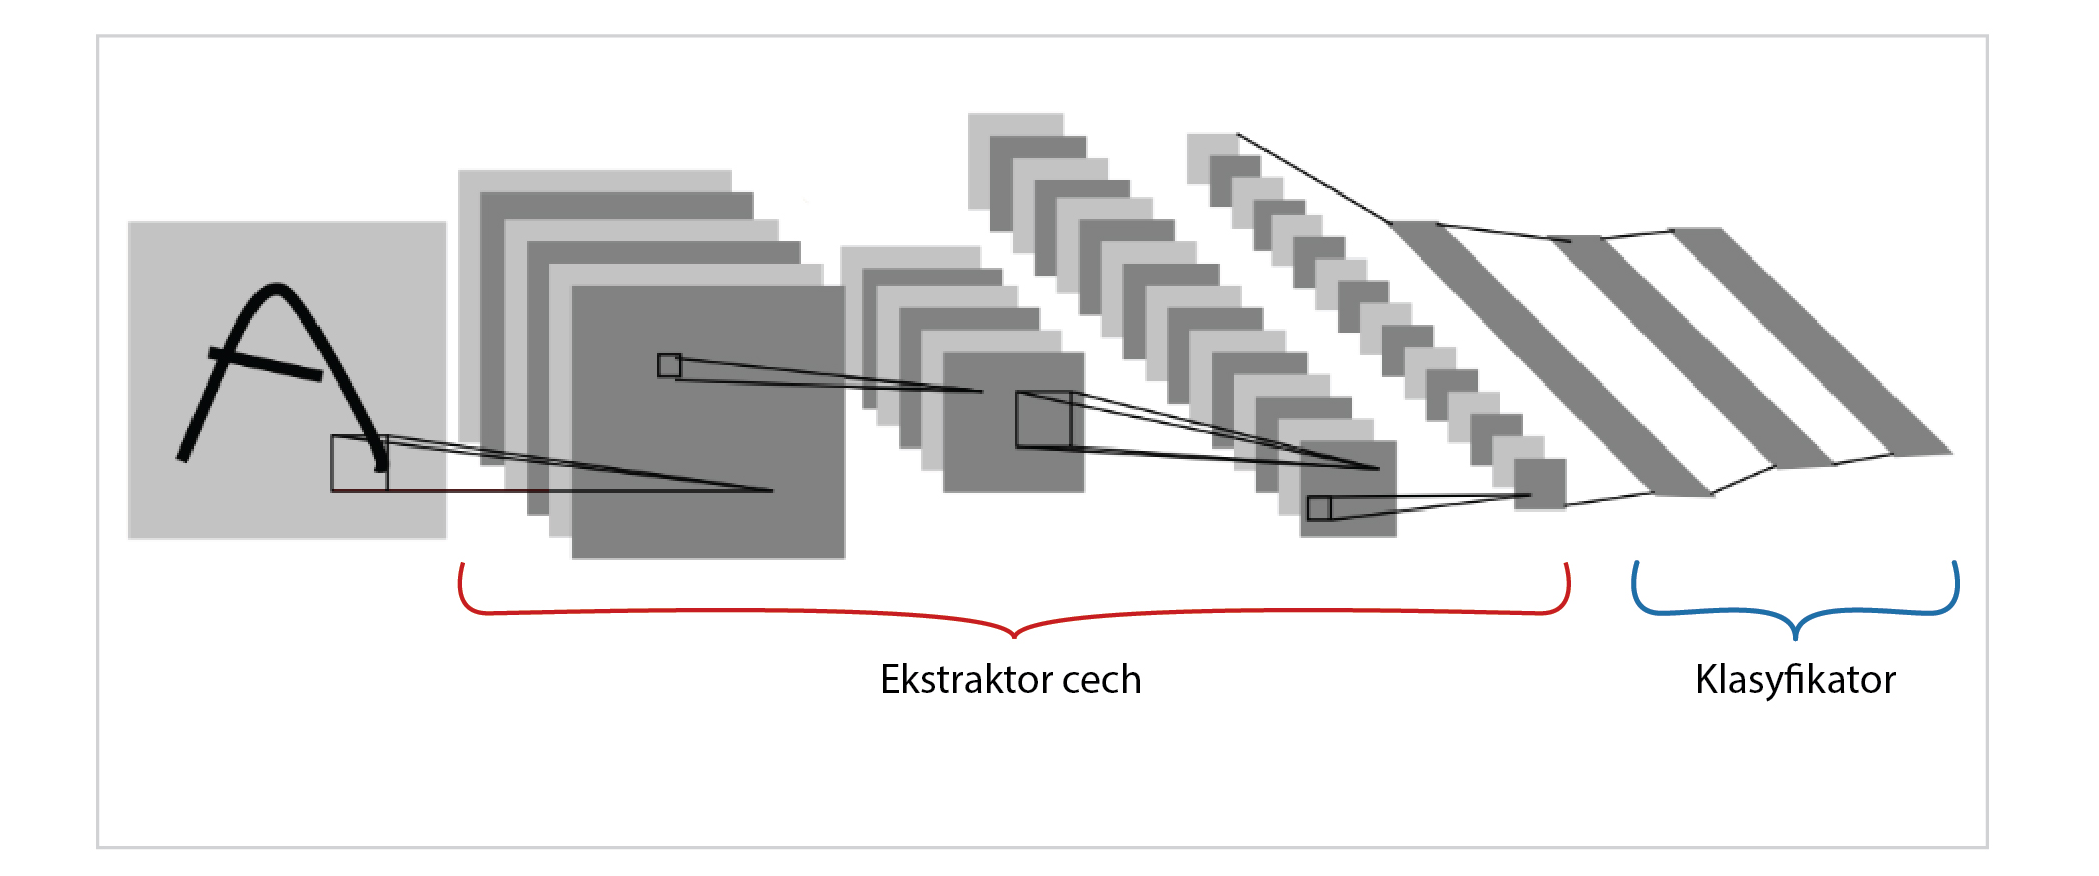
\includegraphics[width=1\textwidth]{figures/lenet.png}
	\caption{Topologia sieci LeNet.}
	\label{LeNet}
\end{figure}

Sieć składa się z 7-miu warstw i zawiera około 60.000 parametrów. Oryginalnie, sygnał wejściowy sieci stanowił obrazek o wymiarach 32$\times$32. W architekturze LeNet zaobserwować można dwie podstawowe składowe współczesnych sieci konwolucyjnych wykorzystywanych do klasyfikacji obrazów tj.:
\begin{itemize}
	\item \textit{ekstraktor cech} -- część służące do automatycznej ekstrakcji wektora cech $w$, zawierająca m.in. filtry.
	\item \textit{klasyfikator} -- część wykorzystywana do zadania wnioskowania końcowego na podstawie $w$.
\end{itemize}  

Przy użyciu takiej architektury możliwe stało się zastosowanie paradygmatu end-to-end learning rozumianego w tym kontekście jako znalezienie w jednym procesie szkolenia się możliwie dobrej transformacji, która surowe obrazy przekształci bezpośrednio w ostateczną klasyfikację. Dokładny opis szkolenia się sieci konwolucyjnych i problemów z tym związanych został przedstawiony w kolejnej sekcji.  

\section{Szkolenie głębokich sieci neuronowych}

Większość algorytmów szkolenia głębokich sieci neuronowych obejmuje zadanie \textit{optymalizacji}, rozumiane jako minimalizację, bądź maksymalizację \textit{funkcji celu} $f$($x$) przez zmianę $x$. W literaturze można też znaleźć inne nazwy funkcji celu takie jak \textit{kryterium}, \textit{funkcja kosztów}, \textit{funkcja strat} lub \textit{funkcja błędów} (por. \cite{Goodfellow-et-al-2016}). 

Podczas zadania optymalizacji bardzo często wykorzystuje się \textit{pochodną funkcji} oznaczaną jako $f'$($x$) lub $\frac{\delta y}{\delta x}$, gdyż niesie ona informacje o nachyleniu funkcji w punkcie $x$. W praktyce funkcje celu są wielowymiarowe dlatego wykorzystywane są \textit{pochodne cząstkowe} informujące o nachyleniu w poszczególnych wymiarach. Wektor zawierający pochodne cząstkowe funkcji nazywany jest \textit{gradientem} i oznaczany jest jako $\bigtriangledown f$($x$). W praktyce wykorzystywane są również: macierz pochodnych cząstkowych tzw. \textit{macierz Jacobiego} oznaczana jako $J$ oraz macierz \textit{drugich pochodnych} cząstkowych (tj. pochodnych pochodnych) tzw. \textit{macierz Hessego} oznaczana jako $H$.

Z uwagi na szybkie znajdowanie lokalnych minimów funkcji celu, to właśnie metody optymalizacji bazujące na wartości gradientu są najczęściej używane w szkoleniu głębokich sieci neuronowych. Inne metody, niegradientowe (zob. \cite{DBLP:journals/corr/TaylorBXSPG16}), przeważnie nie są w tym kontekście wystarczająco efektywne. 

Znalezienie lokalnego minimum nie jest zwykle równoważne z otrzymaniem najlepszego możliwego rozwiązania, jednak w praktyce uznawane jest za satysfakcjonujące. Dla potwierdzenia można przytoczyć następujące fakty wynikające z wielu badań (por. \cite{DBLP:journals/corr/ChoromanskaHMAL14}):
\begin{enumerate}
	\item Dla sieci neuronowych o dużych rozmiarach większość lokalnych minimów charakteryzuje się podobnymi wartościami, przekładającymi się na porównywalny efekt wnioskowania końcowego.
	\item Prawdopodobieństwo znalezienia lokalnego minimum, którego implikacją będą niezadowalające rezultaty wnioskowania przy użyciu sieci maleje wraz ze wzrostem rozmiaru sieci.
	\item Próba znalezienia globalnego minimum bardzo często prowadzi do problemu nadmiernego dopasowania, omówionego dokładniej w sekcji \ref{sec-overffiting}.
\end{enumerate}

Podsumowując, metody gradientowe są wydajne obliczeniowo i prowadzą do znalezienia wielu satysfakcjonujących rozwiązań, które mogą być wykorzystane do rozwiązania praktycznych problemów. 

Zasada działania metod gradientowych bazuje na obieraniu w kolejnych krokach iteracji następujących wartości funkcji $f$, przesuwając się w kierunku spadku gradientu:
\begin{equation}
x' = x - \epsilon \bigtriangledown f(x),
\end{equation} 
gdzie $\epsilon$ to \textit{szybkość uczenia się} -- parametr określający wielkość kroku. 

Funkcja celu w przypadku praktycznych zadań optymalizacyjnych, wykorzystujących głębokie uczenie się jest \textit{funkcją złożoną}, a zatem efekt jej działania jest równoważny operacjom wykonywanym przez kilka lub więcej funkcji po kolei. W takich sytuacjach do obliczeń spadku gradientu wykorzystywane są funkcje, których pochodne są znane.

Aplikuje się je do tzw. \textit{reguły łańcuchowej}. Przypuśćmy, że $v$ = $g$($p$) i $u$ = $f$($g$($p$)) = $f$($v$), gdzie $p$ i $v$ to wektory. Wówczas regułę łańcuchową można zapisać jako:
\begin{equation}
\frac{\delta u}{\delta p_i} = \sum_{j} \frac{\delta u}{\delta v_j} \frac{\delta v_j}{\delta p_i}, 
\end{equation}
co w zapisie wektorowym równoważne jest z równaniem:
\begin{equation}
\label{regLancuch}
\bigtriangledown_x u = (\frac{\delta v}{\delta p})^T \bigtriangledown_q u, 
\end{equation}
gdzie $\frac{\delta v}{\delta p}$ to macierz Jacobiego. 

Regułę łańcuchową zapisaną w \ref{regLancuch} prosto uogólnia się do zmiennych tensorowych (zob. \cite{Goodfellow-et-al-2016}, str. 205) i stosuje się w różnych meta-algorytmach służących do szkolenia sieci. Przykładem jest \textit{algorytm propagacji wstecznej}, który oblicza regułę łańcuchową w wydajnej kolejności stosując działania w grafie takim jak topologia perceptronu wielowarstwowego (zob. \cite{Goodfellow-et-al-2016}).

Proces szkolenia się sieci ma na celu najlepsze możliwe przybliżenie docelowej klasyfikacji bazując na danych przykładach, czyli \textit{zbiorze uczącym} $U$. Algorytmy optymalizacyjne używane do szkolenia głębokich sieci neuronowych zazwyczaj działają pośrednio, optymalizując pewną miarę wydajności $P$, która jest zdefiniowana na \textit{zbiorze testowym}, zawierającym przykłady inne niż w $U$. Często bierze się również pod uwagę dodatkowy podzbiór, rozłączny z $U$ i $T$ -- \textit{zbiór walidacyjny}, który ma pomóc w wyborze najlepszych algorytmów i wartości parametrów wpływających na jakość szkolenia sieci.

W procesie szkolenia zmniejszana jest wartość funkcji kosztów $f$ w oparciu o $U$, a celem jest poprawa $P$. Algorytmy optymalizacyjne wykorzystujące cały zbiór $U$ do liczenia wartości gradientu nazywane są \textit{pakietowymi} lub \textit{deterministycznymi}, gdyż przetwarzają jednocześnie wszystkie przykłady szkoleniowe. Te, które używają jednego przykładu na raz są nazywane \textit{stochastycznymi}. Natomiast w praktyce przy szkoleniu głębokich sieci stosowane są algorytmy \textit{minipakietowe}, wykorzystujące więcej niż jeden przykład, ale mniej niż cały zbiór. Z reguły są to liczby z przedziału 8--256. Takie podejście zapewnia kompromis między szybkością obliczeń a dokładnością estymacji wartości gradientu.

Przykładem algorytmu minipakietowego jest \textit{stochastyczny spadek gradientu} (ang. \textit{stochastic gradient descent}, SGD). Bazuje on na założeniu, że estymację gradientu można otrzymać wyliczając średnią gradientu z minipakietu $m$ przykładów. Kolejne kroki algorytmu można zapisać następująco:
\begin{enumerate}
	\item Wybierz wartość parametru szybkości uczenia się $\epsilon_k$.
	\item Wybierz minipakiet złożony z $m$ przykładów ze zbioru szkoleniowego.
	\item Oblicz estymację gradientu $g$ = $\frac{1}{m}\bigtriangledown \sum_{i=1}^{m}L(x_i, y_i, f)$, gdzie $L$ to funkcja strat dla jednego przykładu o wejściowej wartości próbki $x_i$ i oczekiwanym wyjściu $y_i$.
	\item Zastosuj aktualizację wartości funkcji celu równą $\epsilon_k g$.
	\item Jeżeli kryterium stopu nie zostało spełnione wróć do kroku 2. 
\end{enumerate}

Kryterium stopu jest najczęściej określone liczbą iteracji lub satysfakcjonującą wartością funkcji $f$. Kwestia optymalnego wyboru parametru $\epsilon_k$ zależy od zadanego problemu. Najczęściej stosowane są metody empiryczne, przy czym zazwyczaj $\epsilon_k$ maleje wraz ze zbliżaniem się do satysfakcjonującego rozwiązania.

Parametry algorytmów szkoleniowych nazywane są \textit{hiperparametrami}, gdyż nie są wyznaczane bezpośrednio w procedurze uczenia się. Strategia nadawania hiperparametrom wartości początkowych jest silnie dyskutowana w literaturze (zob. \cite{Koch2017AutomatedHT}) i jej kompleksowy opis wykracza poza zakres tej pracy. Warto jednak wspomnieć o algorytmach z adaptacyjną szybkością uczenia się, gdyż jest to jeden z najtrudniejszych do ustawienia, a jednocześnie bardzo istotny hiperparametr. Do tych algorytmów należą m.in.:
\begin{itemize}
 \item Adaptive Gradient Algorithm (AdaGrad) \cite{Duchi:2011:ASM:1953048.2021068} -- wykorzystywany do indywidualnej adaptacji szybkości uczenia się wszystkich parametrów modelu, skalując je odwrotnie proporcjonalnie do pierwiastka kwadratowego sumy wszystkich historycznych kwadratów gradientów.
 \item Root Mean Square Propagation (RMSProp) \cite{SCHMIDHUBER201585} -- modyfikacja AdaGrad, w której zamiast akumulacji gradientu wykorzystuje się wykładniczo ważoną ruchomą średnią z gradientu.
 \item Adaptive moments algorithm (Adam) \cite{DBLP:journals/corr/KingmaB14} -- W porównaniu z RMSProp, Adam poza momentem pierwszego rzędu (tj. średnią) wykorzystuje również moment drugiego rzędu (tj. \textit{wariancję}). Dokładniej rzecz biorąc, w algorytmie liczona jest wykładnicza ruchoma średnia gradientu i kwadrat z gradientu oraz parametry $\beta_1$ i $\beta_2$, które kontrolują zakres liczenia średnich.
\end{itemize}
W momencie pisania tej pracy, algorytm Adam jest najczęściej rekomendowany jako domyślna metoda szkolenia głębokich sieci neuronowych, dlatego poniżej zamieszczono jego dokładny opis:
\begin{enumerate}
	\item Wybierz wartość początkową $\epsilon$, $\beta_1$, $\beta_2$ oraz ustaw początkowe wartości zmiennych momentu 1 i 2 stopnia $s$ = 0 i $r$ = 0, wartość kroku czasowego $t$ = 0 i stałą $\sigma$ używaną do stabilizacji numerycznej.
	\item Wybierz minipakiet złożony z $m$ przykładów ze zbioru szkoleniowego.
	\item Oblicz estymację gradientu $g$ = $\frac{1}{m}\bigtriangledown \sum_{i=1}^{m}L(x_i, y_i, f)$ i zwiększ $t$ o 1.
	\item Aktualizuj estymację pierwszego momentu. $s$ $\mapsto$ $\beta_1$$s$ + (1-$\beta_1$)$g$.
	\item Aktualizuj estymację drugiego momentu. $r$ $\mapsto$ $\beta_2$$r$ + (1-$\beta_2$)$g\bigodot g$, gdzie $\bigodot$ to iloczyn skalarny dwóch gradientów.
	\item Skoryguj obciążenie momentu pierwszego rzędu $s$ = $\frac{s}{1-\beta_1^t}$.
	\item Skoryguj obciążenie momentu drugiego rzędu $r$ = $\frac{r}{1-\beta_2^t}$.
	\item Zastosuj aktualizację wartości funkcji celu równą -$\epsilon$$\frac{s}{\sqrt{r}+\sigma}$.
	\item Jeżeli kryterium stopu nie zostało spełnione wróć do kroku 2. 
\end{enumerate}

Ocena procesu szkolenia się sieci polega na obliczeniu odpowiednich miar i współczynników odzwierciedlających przybliżenie zbioru $T$ albo $W$ przez znalezione rozwiązanie. W powszechnym problemie klasyfikacji binarnej, występującym również w tej pracy, w kontekście oceny efektywności algorytmów można wyszczególnić opisane poniżej parametry i miary.

Parametry:
\begin{itemize}
	\item \textit{Fałszywie dodatnia klasyfikacja} (\textit{FP} od ang. \textit{False Positive}) -- liczba obserwacji zaklasyfikowanych jako pozytywne, a należących do klasy obserwacji negatywnych.
	\item \textit{Fałszywie ujemna klasyfikacja} (\textit{FN} od ang. \textit{False Negative}) -- liczba obserwacji zaklasyfikowanych jako negatywne, a należących do klasy obserwacji pozytywnych. 
	\item \textit{Prawdziwie pozytywna klasyfikacja} (\textit{TP} od ang. \textit{True Positive}) -- liczba wyników poprawnie zaklasyfikowanych jako pozytywne. 
	\item \textit{Prawdziwie negatywna klasyfikacja} (\textit{TN} od ang. \textit{True Negative}) -- liczba wyników poprawnie zaklasyfikowanych jako negatywne.
\end{itemize}

Miary:
\begin{itemize}
	\item \textit{Dokładność klasyfikacji} (ang. \textit{Accuracy}) -- $ACC = \frac{TP + TN}{TP+TN+FP+FN}$.
	\item \textit{Czułość klasyfikacji} (ang. \textit{Sensitivity}) -- $TPR = \frac{TP}{TP + FN}$.
	\item \textit{Swoistość klasyfikacji} (ang. \textit{Specificity}) -- $TNR = \frac{TN}{TN + FP}$.
	\item \textit{Wartość predykcyjna dodatnia} (ang. \textit{Precision}) -- $PPV = \frac{TP}{TP + FP}$.
	\item \textit{Wartość predykcyjna ujemna} (ang. \textit{Negative precision}) -- $NPV = \frac{TN}{TN + FN}$.
\end{itemize}

W problemach empirycznych dąży się do maksymalizowania TP, TN, ACC, TPR, TNR, PPV i NPV oraz minimalizowania FP i FN. Prawidłowe podejście polega również na wybraniu możliwie efektywnej architektury sieci. Problemy z tym związane zostaną omówione w kolejnych podsekcjach.

\subsection{Problem nadmiernego dopasowania}
\label{sec-overffiting}

Dążenie do najlepszego możliwego przybliżenia zbioru $U$ wprowadza niepożądane zjawisko zwane \textit{nadmiernym dopasowaniem}. Wtedy to dokładność klasyfikacji zbioru $U$ jest wysoka lub nawet bezbłędna, natomiast znacznie niższa jest dokładność klasyfikacji zbioru testowego $T$ i walidacyjnego $W$. W praktyce oznacza to, że model staje się mało użyteczny, gdyż wnioskowanie na nowych danych charakteryzuje się niską dokładnością.

Zatem ogólnym dążeniem w procesie szkolenia się sieci jest osiągnięcie \textit{maksymalnej generalizacji} klasyfikacji. Sieć o wysokim współczynniku generalizacji lepiej klasyfikuje ogół zadanych wektorów wejściowych niż sieć, która ma niski współczynnik generalizacji i jest nadmiernie dopasowana do zbioru $U$. Właściwym działaniem jest ustalenie maksymalnie ogólnych, dostatecznych warunków poprawnej klasyfikacji, dzięki którym wzrasta prawdopodobieństwo, że przykład spoza zbioru $U$ będzie poprawnie klasyfikowany. W tym celu można zastosować \textit{metodę oceny krzyżowej} (ang. \textit{cross-validation}). Metoda ta polega na podziale zbioru uczącego na $s$ segmentów $D$, z których każdy w innej iteracji służy jako zbiór testujący i walidacyjny, a pozostałe segmenty pełnią rolę zbioru uczącego. Podział zobrazowany jest na Rysunku \ref{cross-validation}.
\begin{figure}[h!]
	\centering
	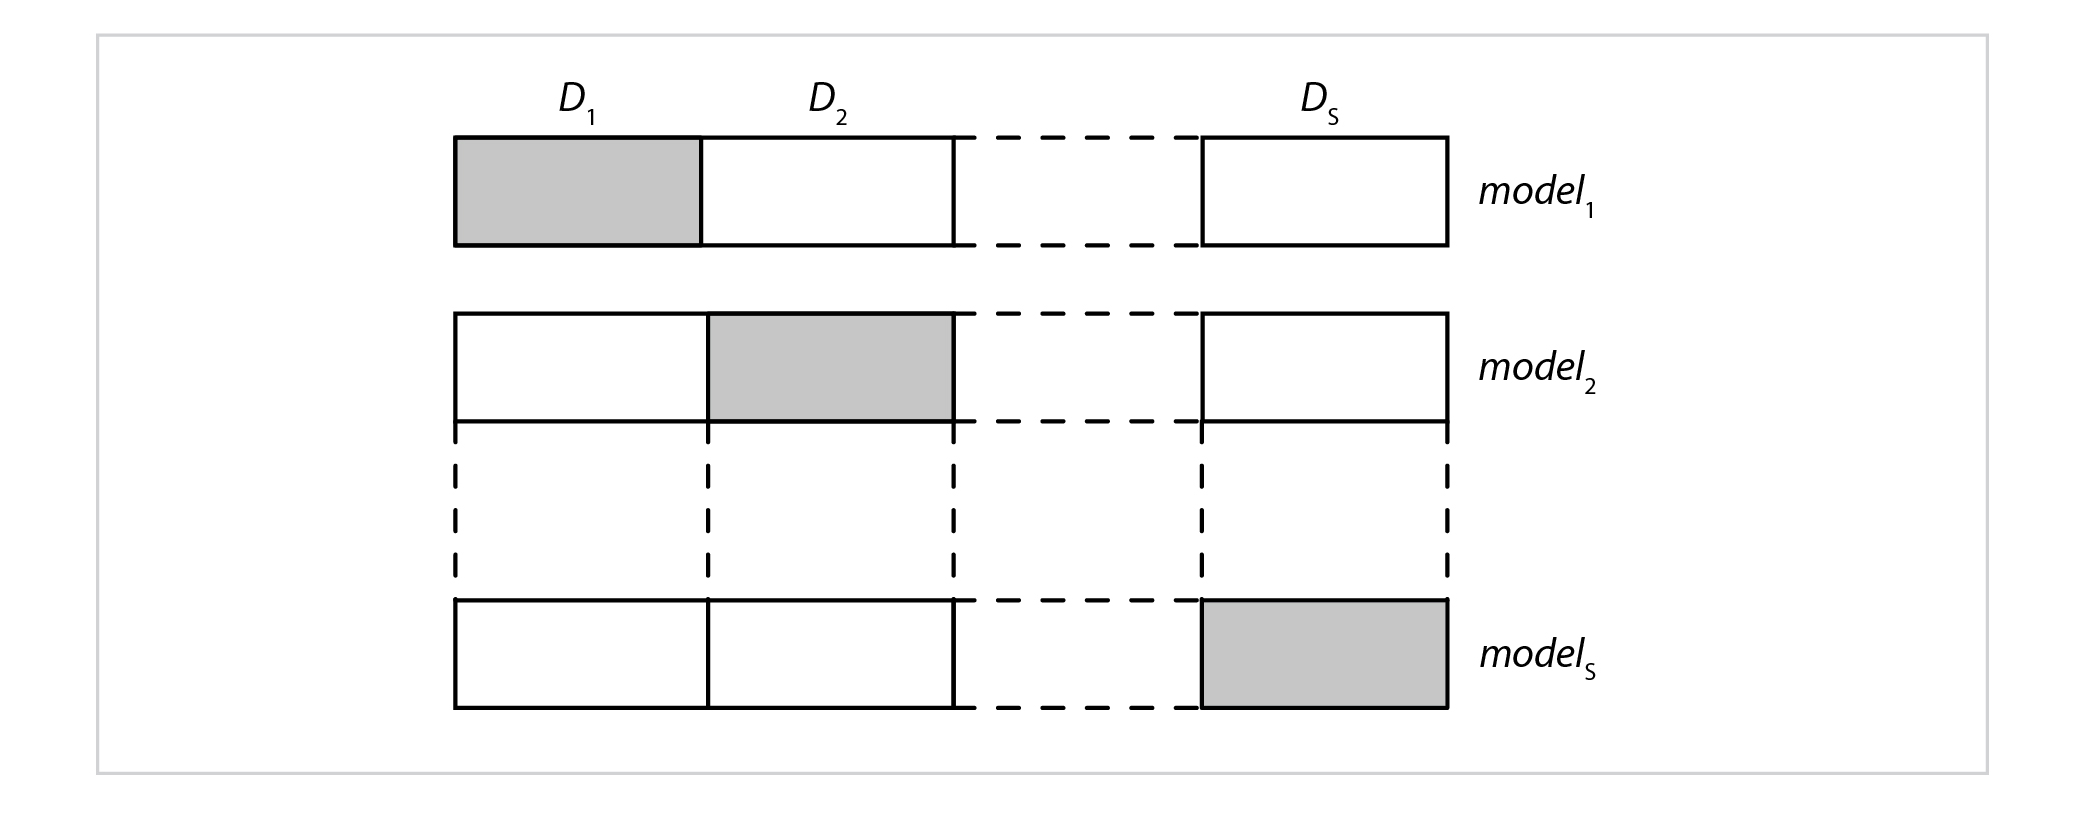
\includegraphics[width=1\textwidth]{figures/cross-validation.png}
	\caption{Reprezentacja graficzna oceny krzyżowej.}
	\label{cross-validation}
\end{figure}
Stosując metodę oceny krzyżowej dla różnych modeli sieci można stwierdzić, który z nich spełnia najlepiej kompromis między dobrą klasyfikacją zbioru $U$ i wysoką generalizacją.

Kombinacja predykcji wielu różnych modeli jest bardzo wydajną metodą stosowaną do polepszenia generalizacji i zmniejszenia błędu klasyfikacji na zbiorach innych niż $U$ (zob. \cite{Bell2007, Breiman2001}). Jednak współczesne sieci neuronowe, których przykłady zostały opisane w dalszych sekcjach, mogą zawierać miliony parametrów i ich optymalizacja jest wymagająca obliczeniowo. Z tego powodu w praktyce ogranicza się liczbę segmentów obierając $s$ $\in$ $\langle$3, 10$\rangle$.

Innym podejściem do zwiększenia generalizacji, zaproponowanym w 2012 w \cite{DBLP:journals/corr/abs-1207-0580}, jest technika \textit{dropout}, której główna idea bazuje na zerowaniu wyjścia neuronów sieci z prawdopodobieństwem 0,5 przy każdej iteracji treningu sieci. Neurony, które są w ten sposób tymczasowo dezaktywowane nie mają wpływu w danej iteracji na predykcję sieci i nie są uwzględniane przy wstecznej propagacji gradientu. Podejście to można porównać do treningu w każdej iteracji różnych modeli sieci. Dla przykładu w \cite{Krizhevsky2012} wykazano, że metoda dropout wymaga jedynie 2 razy więcej iteracji do przybliżenia zbioru $U$, przy czym uzyskuje znacznie lepszą generalizację. 

Kluczowym składnikiem potrzebnym do treningu sieci i maksymalizacji generalizacji jest odpowiedni rozmiar zbioru danych. Jest to problem szeroko dyskutowany, gdyż zwłaszcza w danych medycznych istnieje szereg ograniczeń związanych z dostępem i akwizycją odpowiedniego materiału badawczego (np. ograniczenia prawne, związane z prywatnością lub z etyką). W przypadku, gdy zgromadzenie odpowiedniego zbioru danych jest niemożliwe, pewnym rozwiązaniem problemu jest zastosowanie metod jego sztucznego powiększania (ang. \textit{data augmentation}).

Dla obrazów stosuje się metody \textit{afinicznych przekształceń} zgodne z definicją algebraiczną:
\begin{equation}
	\mathbf o \mapsto \mathbf{Ao} + \mathbf b,
\end{equation}
gdzie $A$ jest macierzą przekształcenia liniowego, a $b$ wektorem przesunięcia. Jako przykłady takich przekształceń dla dwuwymiarowych obrazów można wymienić:
\begin{itemize}
	\item \textit{rotację} -- obrót obrazu o kąt $\theta$, gdzie:
	\begin{equation}
	A = \begin{bmatrix} 
	\cos \theta & \sin \theta\\
	-\sin \theta & \cos \theta
	\end{bmatrix}
	\end{equation}	
	\item \textit{odbicie lustrzane} -- odwrócenie kolejności pikseli w każdym wierszu, gdzie:
	\begin{equation}
		A = \begin{bmatrix} 
		-1 & 0\\
		0 & 1
	\end{bmatrix}
	\end{equation}
	\item \textit{skalowanie} -- zmiana rozmiaru obrazu o $S$, gdzie:
	\begin{equation}
			A = \begin{bmatrix} 
		S_x & 0\\
		0 & S_y
	\end{bmatrix}
	\end{equation}
	\item \textit{translację} -- przesunięcie punktów obrazu o wektor $b$.
\end{itemize}

Analogiczne równania istnieją dla obrazów trójwymiarowych (zob. \cite{Hill06}). W określonych przypadkach używane są również nieafiniczne przekształcenia. Dla przykładu, w \cite{DBLP:journals/corr/RonnebergerFB15} wykorzystano nieliniowe deformacje do powiększenia zbioru 30-tu obrazów mikroskopowych przedstawiających macierz komórkową i uzyskano znacząco lepsze wyniki detekcji komórek od istniejących w 2015 r. najlepszych rozwiązań.

Dla danych medycznych należy szczególnie zwrócić uwagę, aby powiększony zbiór zawierał dane przypominające przypadki występujące w rzeczywistości np. nieduże obroty występujące u pacjentów skanowanych Rezonansem Magnetycznym lub niewielkie skalowania rozmiaru kości widocznych w Tomografii Komputerowej. Szeroka dyskusja prowadzona się również na temat wykorzystania sztucznie generowanych zbiorów danych o czym więcej można przeczytać w \cite{DBLP:journals/corr/SixtWL16, Litjens2017}. 

\subsection{Problem redukcji wymiarowości}
\label{DimReduction}
Duży rozmiar wektora cech prowadzi do problemu nazwanego \textit{przekleństwem wymiarowości} (ang. \textit{curse of dimensionality}). Określenie zostało po raz pierwszy sformułowane przez Richarda Bellmana w latach 50-tych XX wieku. Naukowiec ten podczas swojej pracy obserwował algorytmy doskonale działające w 3 wymiarach, a prezentujące znacząco gorsze wyniki w hiperprzestrzeni (zob. \cite{Bellman:1957}). 

Problem przekleństwa wymiarowości ma dwie główne przyczyny: (1) nie wszystkie cechy są jednakowo znaczące w kontekście rozróżnienia danych; (2) w miarę wzrostu rozmiaru przestrzeni cech, liczba obserwacji w zbiorze uczącym potrzebnych do wiarygodnego oszacowania funkcji wyjściowej rośnie wykładniczo.  

Problem (1) jest szczególnie istotny w dość prostych algorytmach takich jak np. algorytm $K$-najbliższych sąsiadów, gdzie do poprawnego działania należy policzyć dystans pomiędzy sąsiednimi obserwacjami. Uwzględniając dużą liczbę nieistotnych cech jako argumenty funkcji dystansu uzyskuje się wyniki utrudniające lub nawet uniemożliwiające poprawną klasyfikację zbioru. Konieczna jest wówczas adaptacja wpływu poszczególnych cech np. poprzez wprowadzenie wektora wag.

Problem (2) ma duże implikacje w praktyce stosowania sieci neuronowych, gdyż uzyskanie odpowiednio dużego, ustrukturyzowanego zbioru danych stanowi przeważnie wyzwanie. W poprzedniej podsekcji omówiono możliwość sztucznego powiększania zbioru danych. Inną opcją jest zmniejszenie rozmiaru wektora cech, co może być wykonane na dwa sposoby:

\begin{itemize}
\item wybór podzbioru istotnych cech o liczności $n'$ $<<$ $n$,
\item przekształcenie oryginalnych $n$ zmiennych na nowy zbiór $n'$ cech, gdzie ponownie $n'$ $<<$ $n$.
\end{itemize}

W pierwszym przypadku, wybór podzbioru istotnych cech polega na określeniu minimalnego podzbioru, dla którego rozkład prawdopodobieństwa różnych klas obiektów jest jak najbliższy oryginalnemu rozkładowi uzyskanemu z wykorzystaniem wszystkich cech. Do tych zagadnień wykorzystywane są metody takie jak:
\begin{itemize}
	\item \textit{miary siły związku} -- określające podobieństwo między rozkładami zmiennych losowych. Najczęściej stosowana jest \textit{korelacja Pearsona}, której współczynnik $r$ dla dwóch zmiennych losowych $X1$ i $X2$ zapisywany jest następującym wzorem:
	\begin{equation}
	r_{X1X2} = \frac{\sum_{i=1}^n (X1_i - \overline{X1})(X2_i - \overline{X2})}{\sqrt{\sum_{i=1}^n (X1_i - \overline{X1})^2} \sqrt{\sum_{i=1}^n (X2_i - \overline{X2})^2}},
	\end{equation}
	gdzie $X1_i$, $X2_i$ to wartości kolejnych obserwacji, a $\overline{X1}$ i $\overline{X2}$ to ich średnie. Innymi słowy tak zapisany współczynnik $r_{X1X2}$ jest ilorazem \textit{kowariancji} i iloczynu \textit{odchyleń standardowych} zmiennych $X1$ i $X2$.
	\item \textit{miary entropii względnej} --  określające rozbieżności między rozkładami zmiennych losowych. Najczęściej stosowana jest \textit{dywergencja Kullbacka-Leiblera}, której współczynnik $d_{KL}$ dla dwóch rozkładów prawdopodobieństwa $p_k$ i $q_k$ zapisany jest wzorem: 
	\begin{equation}
	d_{KL}(p_k, q_k) = \sum_{i} p_k(i) \log_2 \frac{p_k(i)}{q_k(i)}
	\end{equation}
	\item \textit{teoria zbiorów przybliżonych} -- wykorzystująca informacje o elementach zbioru i klasyczną teorię zbiorów do porównywania rozkładów (zob. \cite{Kowalik2003}).
\end{itemize}
Podobieństwo rozkładów ocenione na podstawie powyższych miar daje możliwość skutecznej redukcji wymiarowości z zachowaniem efektywności algorytmu.

W celu selekcji cech można również stosować różnego rodzaju, specjalnie zaprojektowane regresje. Do najbardziej powszechnie stosowanych należą algorytmy regresji grzbietowej, LASSO (od ang. \textit{Least Absolute Shrinkage and Selection Operator}) oraz Elastic Net. Różnią się one definicją zadania minimalizacji wektora cech $w$:

\begin{equation}
\textrm{Regresja grzbietowa-- } \underset{w}{min} ||X*w-Y||_2^2 + \alpha ||w||_2^2;
\label{equ:ridgeReg}
\end{equation}
\begin{equation}
\textrm{LASSO-- } \underset{w}{min} ||X*w-Y||_2^2 + \alpha ||w||_1;
\label{equ:lassoReg}
\end{equation}
\begin{equation}
\textrm{Elastic Net-- } \underset{w}{min} { \frac{1}{2n_{samples}} ||X w - y||_2 ^ 2 + \alpha \rho ||w||_1 + \frac{\alpha(1-\rho)}{2} ||w||_2 ^ 2}.
\label{equ:elasticNet}
\end{equation}

W szczególności istotny jest czynnik regulujący dołączony do klasycznego zadania regresji liniowej będący pierwszym elementem każdego zadania minimalizacji. W regresji grzbietowej dodatkowo dodawany jest warunek minimalizacji \textit{Normy L2} z wektora $w$ ($\left \| w \right \|_2 =\sqrt{ \sum_{k=1}^{n}\left |w_k  \right |^2}$), dzięki czemu wymuszane jest, aby poszczególne współczynniki nie były za duże. W regresji LASSO stosowana jest \textit{Norma L1}, ($\left \| w \right \|_1 = \sum_{k=1}^{n}\left |w_k  \right |$), dzięki czemu preferowane są rozwiązania, w których wektor jest rzadki, co przekłada się na efektywny wybór cech z grup silnie skorelowanych. Regresja Elastic Net łączy w sobie cechy regresji grzbietowej oraz LASSO, poprzez zastosowanie dwóch typów norm jednocześnie, których istotność względem siebie kontroluje parametr $\rho$. Minusem tego podejścia jest większa złożoność obliczeniowa i konieczność doboru wartości dodatkowego parametru. Z uwagi na definicję zadania minimalizacji, powyższe algorytmy znajdują zastosowania głównie w problemach, gdzie występują zależności liniowe. Do nieliniowych problemów stosuje się częściej bardziej skomplikowane algorytmy typu lasy losowe.

W kolejnym omawianym przypadku, tj. gdy zaistnieje potrzeba przekształcenia przestrzeni cech i wyliczenia nowego zbioru, metodą \textit{state-of-the-art} jest algorytm \textit{analizy składowych głównych} (ang. \textit{Principal Component Analysis}, w skr. \textit{PCA}) opracowany przez Karla Pearsona w 1901 r (zob. \cite{PCA}).  

Istotą PCA jest przekształcenie początkowych, skorelowanych cech w nowy zbiór nieskorelowanych zmiennych. Nowe zmienne, tzw. \textit{składowe główne} lub \textit{czynniki główne}, powstają z przekształcenia oryginalnych zmiennych skorelowanych w taki sposób, aby w maksymalnym stopniu wyjaśniać całkowitą wariancję w próbie cech oryginalnych. Wariancje składowych głównych są \textit{wartościami własnymi} macierzy kowariancji oryginalnych zmiennych. Innymi słowy są to \textit{wartości skalarne} (pojedyncze liczby) opisujące poziom wariancji w danych w stosunku do zadanych \textit{ortogonalnych wektorów}, tj. takich, dla których iloczyn skalarny równy jest 0, co w przestrzeni Euklidesowej oznacza, że kąt pomiędzy wektorami równy jest 90$^\circ$.

Dla przykładu, pierwsza składowa główna redukuje największą część zróżnicowania, druga kolejną, której nie redukowała poprzednia itd. Składowych głównych jest zawsze tyle ile wymiarów danych. Przykład dwuwymiarowy został przedstawiony na Rys. \ref{PCA-2dim}.
\begin{figure}[h!]
	\centering
	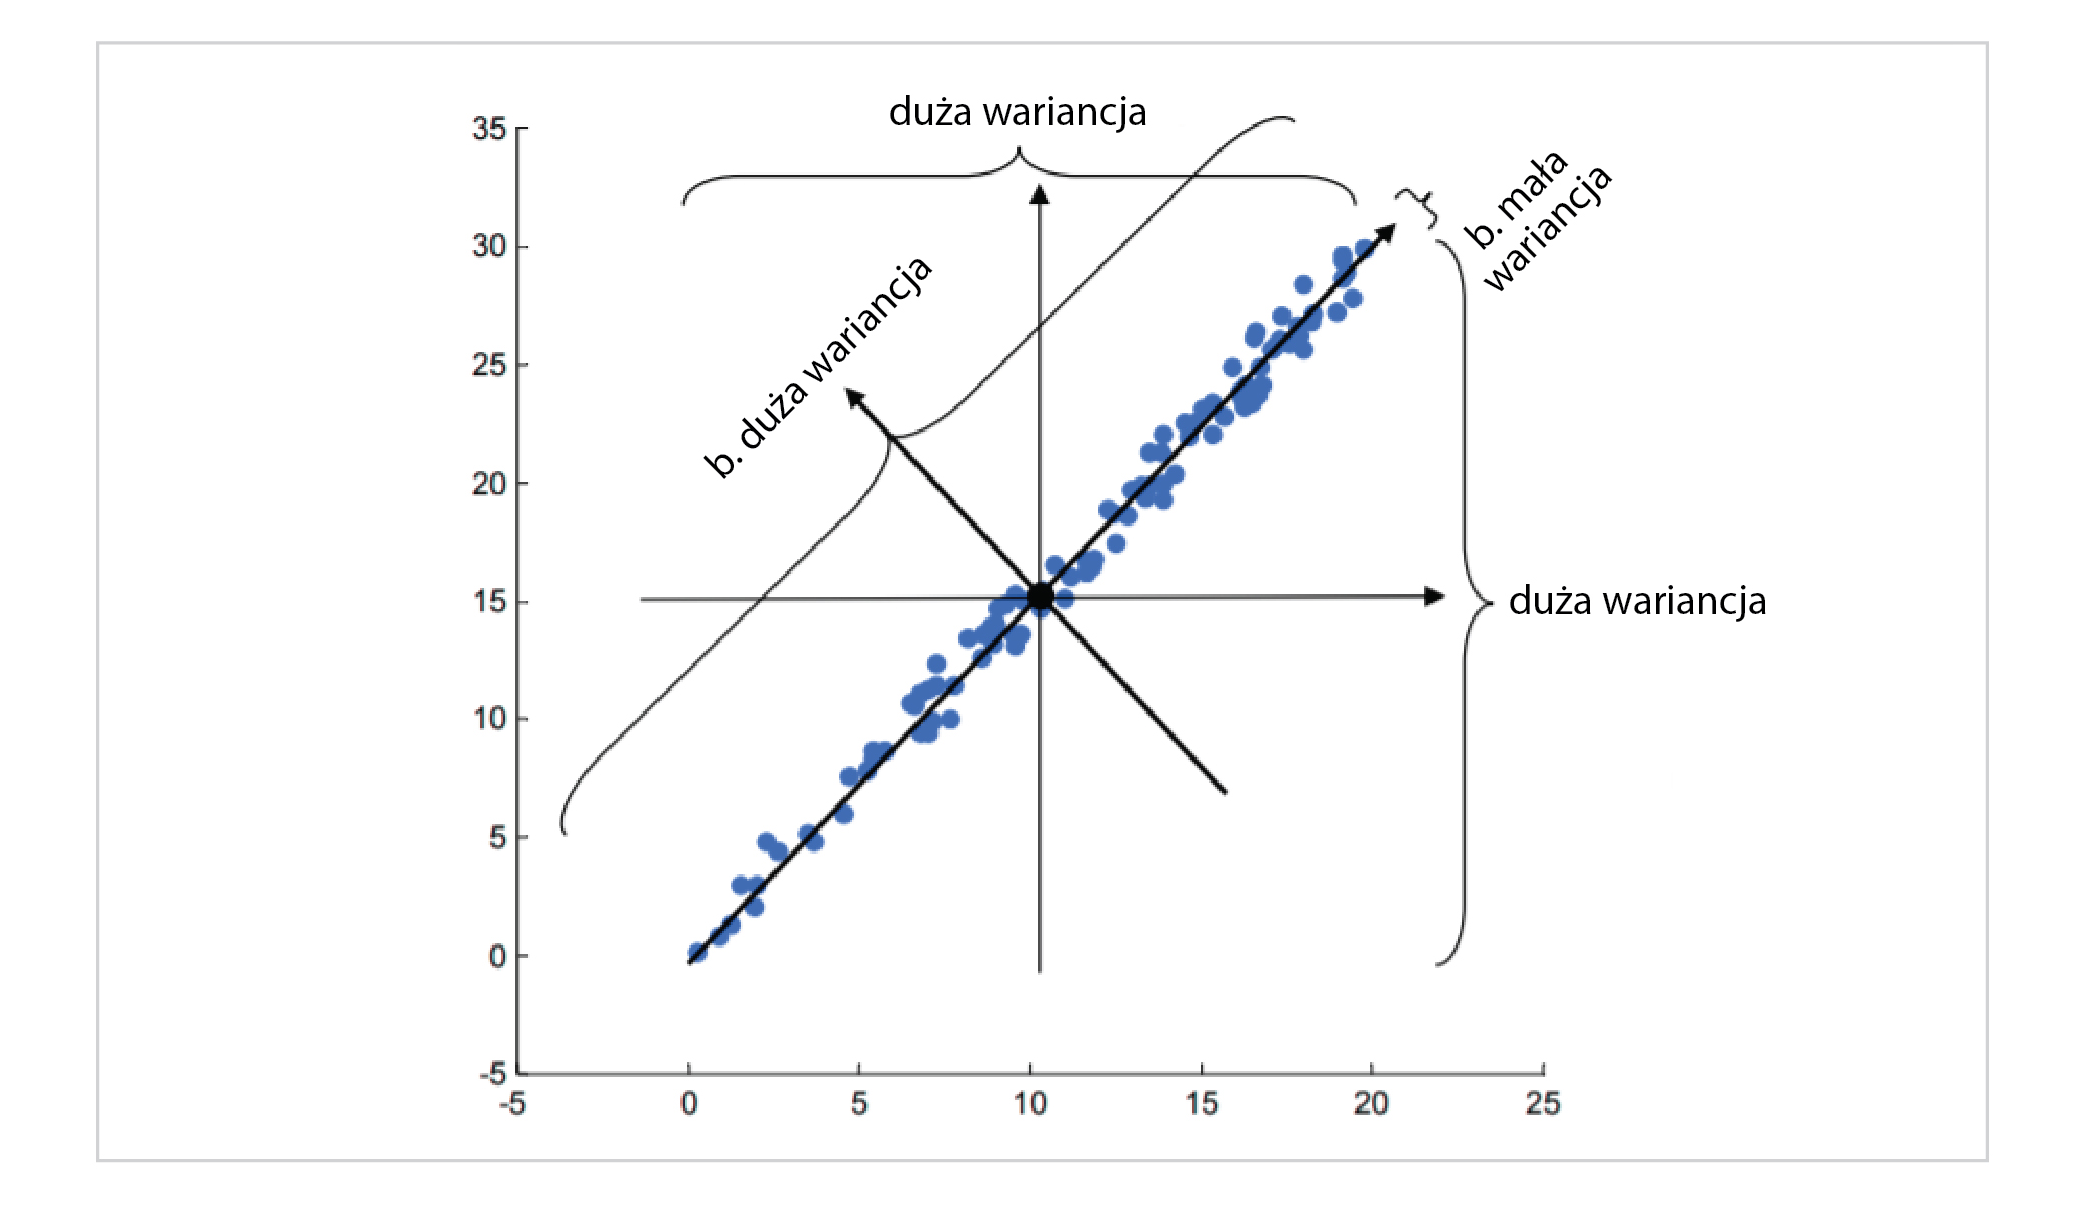
\includegraphics[width=1\textwidth]{figures/PCA.png}
	\caption{Dwuwymiarowa przestrzeń cech wraz z zaznaczonymi poziomami warianci i składowymi głównymi.}
	\label{PCA-2dim}
\end{figure}
Można zaobserwować, że nowa przestrzeń charakteryzuje się znacznie większym zróżnicowaniem poziomu wariancji niż przestrzeń oryginalna. Wybierając zatem tylko pierwszą składową uzyskana zostanie reprezentacja \textit{skomprymowana stratnie} (tzn. taka, która nie daje gwarancji odtworzenia oryginalnych wartości), ale za to zachowująca znaczną część wariancji.

Opis szczegółowej procedury PCA wygląda następująco:
\begin{enumerate}
\item Oblicz macierz kowariancji: $S_x$ = $X^{T}X$, gdzie $X$ to macierz danych zawierająca obserwacje w wierszach. Macierz $S_x$ jest symetryczna i pozwala ocenić: (1) wariancje zmiennych poprzez analizę elementów na głównej przekątnej; (2) zależności pomiędzy zmiennymi poprzez analizę elementów poza główną przekątną. 
\item Dokonaj diagonalizacji: $S_x$ = $KLK^{-1}$, gdzie $L$ to macierz diagonalna, a $K$ to macierz odwracalna składająca się z wektorów własnych odpowiadających kolejnym wartościom własnym.
\item Utwórz macierz nowych zmiennych wykonując operację: $Y$ = $XK$
\end{enumerate}

Oprócz PCA, w kontekście redukcji wymiarowości, można również wyróżnić następujące algorytmy: 
\begin{enumerate}
	\item \textit{Multidimensional scaling}, MDS -- bazuje na wyliczeniu odpowiednio zdefiniowanego dystansu między wartościami cech w oryginalnej przestrzeni i próbie zachowania tego dystansu w zredukowanej wymiarowości (zob. \cite{Chen:2008:HDV:1370965}).
	\item \textit{T-distributed stochastic neighbor embedding}, t-SNE -- stosowany do wizualizacji struktur cech w różnych skalach (zob. \cite{vanDerMaaten2008}).
	\item \textit{Isomap} -- algorytm nieliniowej redukcji wymiarowości pozwalający na gwarantowane znalezienie globalnego minimum (zob. \cite{tenenbaum_global_2000}). 
	\item \textit{Independent Component Analysis}, ICA -- stosowany do znalezienia reprezentacji danych składających się z niezależnych elementów (zob. \cite{ICA}).
	\item \textit{Latent Semantic Analysis}, LSA -- stosowany głównie w problemach dotyczących przetwarzania języka naturalnego, zwłaszcza do znalezienia kontekstu użycia danego słowa poprzez analizę statystyczną dużych bloków tekstów (zob. \cite{Wolfe2003}). 
	\item \textit{Self Organizing Maps}, SOM --  bazuje na zachowaniu własności topologicznych przestrzeni cech oryginalnych w zredukowanej wymiarowości (zob. \cite{Vesanto00self-organizingmap}).
\end{enumerate}

Zarówno przekleństwo wymiarowości, jak i wcześniej opisany problem nadmiernego dopasowania są zjawiskami bardzo często występującymi w praktycznych zastosowaniach algorytmów głębokiego uczenia się. Nie wyczerpują one jednak tematu. Szereg kolejnych wyzwań i rozwiązań został opisany w kolejnej sekcji przy okazji przedstawienia współczesnych topologii.

\section{Przykłady współczesnych topologii}

Współczesne sieci konwolucyjne służące do klasyfikacji obrazów, podobnie jak u protoplasty tj. architektury LeNet, składają się z dwóch głównych części: ekstraktora cech i klasyfikatora. W porównaniu jednak do pierwszych topologii, różnorodność warstw uległa zwiększeniu. Do najczęściej stosowanych komponentów można zaliczyć:
\begin{itemize}
	\item \textit{warstwy konwolucyjne} -- grupują filtry używane do ekstrakcji cech obrazowych różnego poziomu (np. krawędzie, skupiska, obiekty);
	\item \textit{warstwy max-pool} -- stosowane do nieliniowej redukcji wymiarowości. Z obszaru $n\times$$n$ w obrazie wyliczana jest największa wartość $I$($x$, $y$). W praktyce zazwyczaj $n$=2, podobnie jak wartość \textit{kroku} tj. odstępu pomiędzy kolejnymi próbkowaniami funkcji $I$. W uzasadnionych przypadkach stosuje się również obliczanie średniej tzw. (\textit{Avg-pool}), Normy $L2$ i innych współczynników;
	\item \textit{warstwy aktywacji} -- zawierające funkcje aktywacji neuronów. We współczesnych architekturach zamiast funkcji sigmoidalnych czy progowych stosuje się najczęściej funkcję ReLU:
	\begin{equation}
		f(x) = \max(0, x).
	\end{equation}
	Jest ona mniej wymagająca obliczeniowo niż funkcja sigmoid, a dla współczesnych topologii o dużej liczbie parametrów testy empiryczne wykazały, że równie dobrze wpływa na uzyskiwane wyniki dokładności (zob. \cite{Krizhevsky2012}); 
	\item \textit{warstwy gęste lub z ang. fully connected}, FC -- składające się z neuronów, z których każdy jest połączony z każdym neuronem kolejnej warstwy. Występują zazwyczaj w ostatniej części sieci konwolucyjnych tj. w klasyfikatorze;
	\item \textit{warstwy normalizacji}\footnote{Coraz rzadziej stosowane w praktyce z uwagi na znikomy wpływ na rezultaty.} -- normalizujące wyjście poprzedzającej warstwy do pewnego określonego przedziału, zazwyczaj (-1,1). Przykładem jest operacja \textit{Local Response Normalization} dana wzorem:
	\begin{equation}
	\label{DLnormEquation}
	b_{x,y}^{i} = a_{x,y}^{i}/\left ( k + \alpha \sum_{j=max(0,i-n/2)}^{min(N-1,i+n/2)}(a_{x,y}^{i})^2 \right )^\beta,
	\end{equation}
	gdzie $a_{x,y}^{i}$ jest aktywacją danego neuronu, a $k$, $\alpha$, $n$ i $\beta$ to stałe dobierane empirycznie na podstawie zbioru walidacyjnego (za \cite{Krizhevsky2012}). Warstwy normalizacji wykorzystywane są w celu zrównoważenia poziomu wpływu poszczególnych neuronów na wynik końcowy.
\end{itemize}

Wprowadzenie w ostatnich latach dedykowanych dla szkolenia się głębokich sieci neuronowych rozwiązań, zarówno w warstwie sprzętowej jak i oprogramowania, umożliwiło tworzenie architektur o wysokim stopniu komplikacji. W głównej mierze rozwiązania te pozwoliły na optymalizację fazy szkolenia (omówionej w poprzedniej sekcji) jak również \textit{fazy wnioskowania}, gdzie wytrenowana sieć użyta jest do przetwarzania kolejnych obserwacji. W warstwie sprzętowej wyróżnić można dedykowane akceleratory do operacji macierzowych, takie jak w \cite{DBLP:journals/corr/abs-1803-04014}, stworzone przez firmę NVIDIA, \textit{Tensor Processing Unit} (w skr. \textit{TPU}) czy opracowane przez firmę Intel procesory Nervana \cite{Intel}. 

W warstwie oprogramowania należy wspomnieć o rozwiązaniach takich jak TensorRT \cite{TensorRT}, które minimalizują czasy przetwarzania sygnału przez wytrenowaną sieć np. stosując optymalizację reprezentacji liczb zmiennoprzecinkowych lub przetwarzanych macierzy. Dynamicznie rozwijają się również frameworki do zoptymalizowanych obliczeń z udziałem głębokich sieci neuronowych np.: Caffe, Caffe2, TensorFlow, Theano, PyTorch czy MXNet. Ich porównanie osadzone w kontekście aplikacji medycznych można znaleźć w \cite{Erickson2017}.

Postęp w rozwoju współczesnych sieci konwolucyjnych doskonale odzwierciedla progres w rezultatach konkursu ImageNet Large Scale Visual Recognition Competition (w skr. ILSVRC) przedstawiony na Rys. \ref{ILSVRC}.
\begin{figure}[h!]
	\centering
	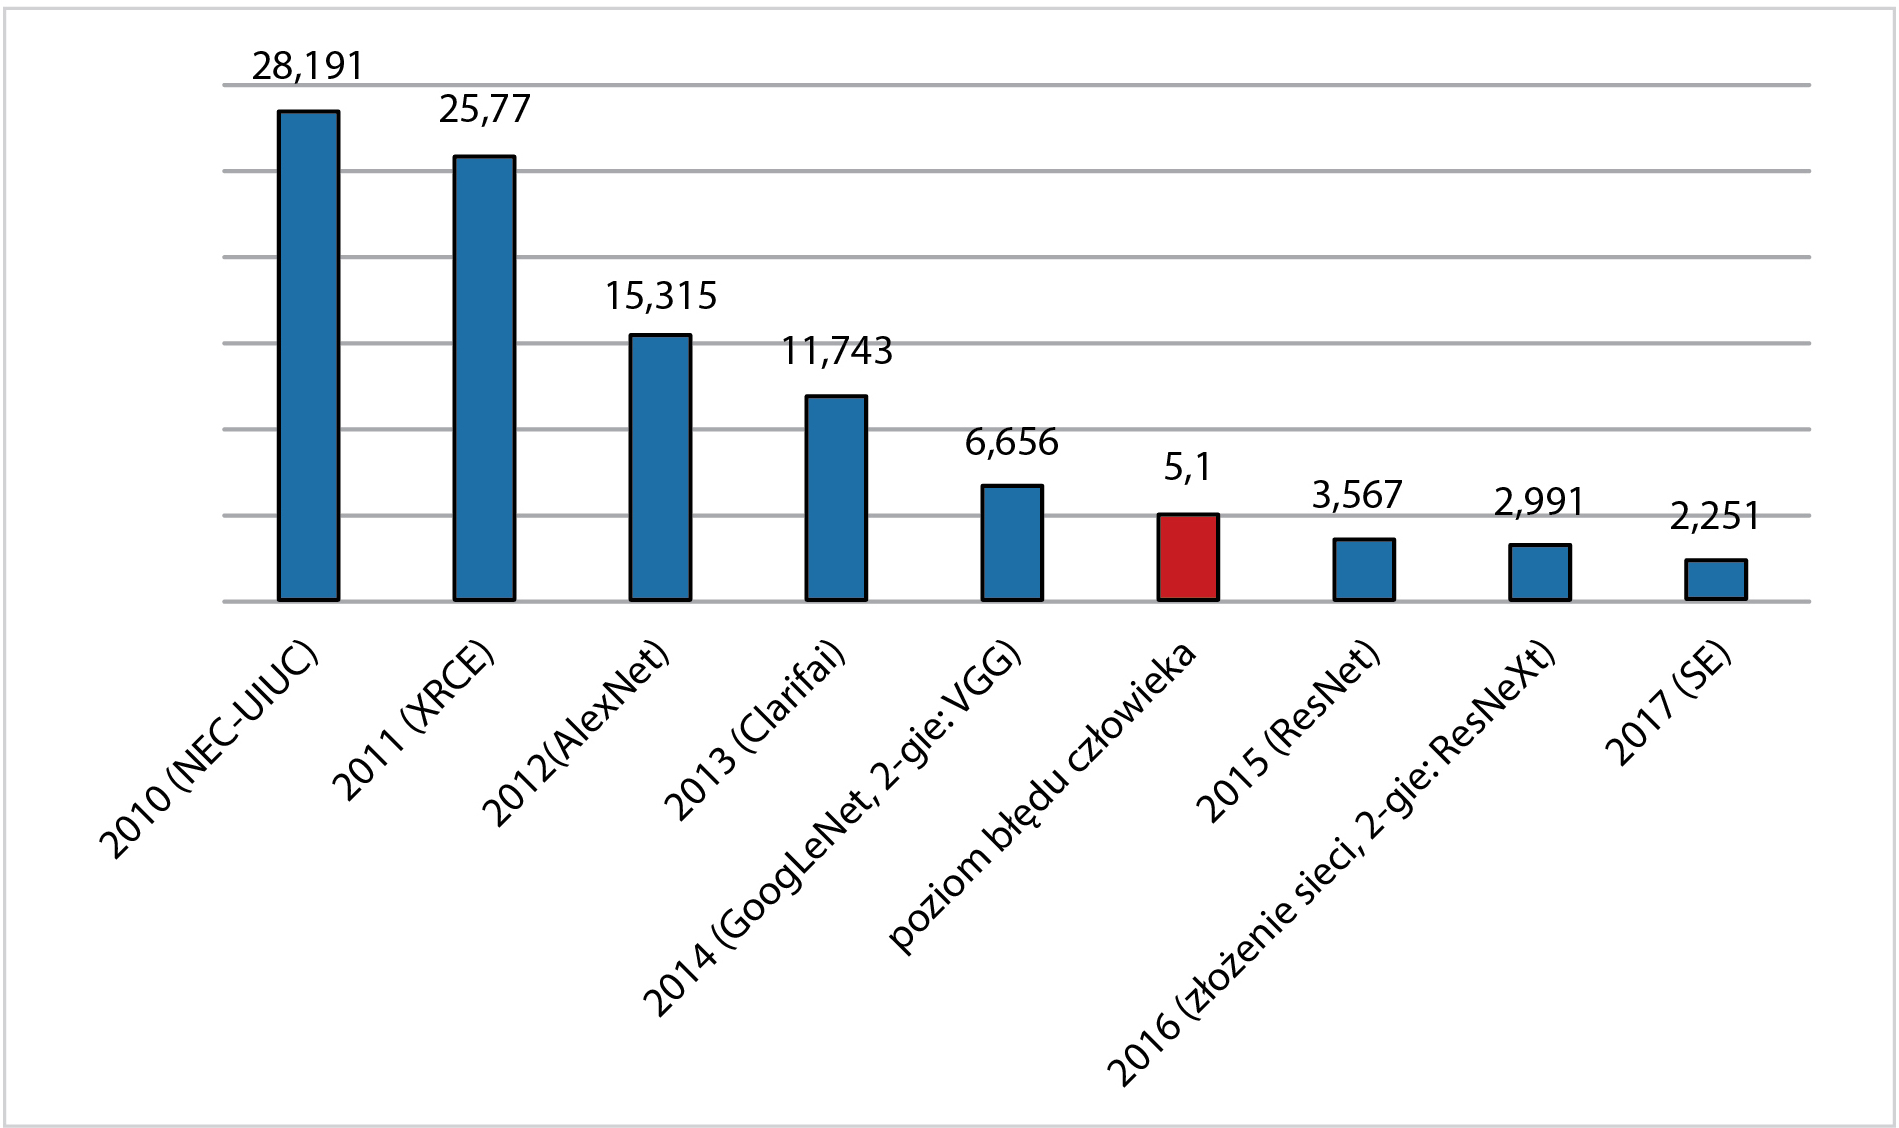
\includegraphics[width=1\textwidth]{figures/ILSVRC.jpg}
	\caption{Błąd top-5 klasyfikacji obiektów w kolejnych latach uzyskiwany przez zwycięzców konkursu ILSVRC}
	\label{ILSVRC}
\end{figure}
Prezentowane wyniki dotyczą wartości błędu klasyfikacji, na zbiorze danych \cite{imagenet_cvpr09} o nazwie ImageNet, uzyskiwanego w kolejnych latach przez zwycięskie algorytmy biorące udział w konkursie. \textit{Błąd top-$n$} należy rozumieć jako zdarzenie, w którym dla danego obrazka w $n$ wskazanych przez algorytm najbardziej prawdopodobnych etykietach nie było poprawnej. W zakresie zmniejszenia wartości błędu top-$n$, znaczący progres dokonał się w 2012 roku, gdzie błąd top-5 zmalał o 10,4 punktów procentowych, co było rezultatem działania nowej architektury sieci konwolucyjnej nazwanej AlexNet. W kolejnych latach sieci konwolucyjne deklasowały inne podejścia, doprowadzając w 2015 roku do spadku błędu top-5 do poziomu 3,5\%, co jest uznawane za poziom lepszy niż możliwości ludzkiej klasyfikacji zbioru ImageNet. Lata 2016--2018 to intensywne prace nad synergią i złożeniami różnego rodzaju modeli, które w konsekwencji doprowadziły do obniżenia wartości błędu top-5 do poziomu 2,2\%. W kolejnych podsekcjach zostanie dokładniej omówiona ewolucja zwycięskich architektur z konkursu ILSVRC. 

\subsection{AlexNet}
\label{AlexNet}
Sieć AlexNet, której nazwa pochodzi od imienia głównego twórcy tej architektury Alexa Krizhevsky, zawiera blisko 60 milionów parametrów i 650 tysięcy neuronów. Architekturę zaprezentowano na Rys. \ref{AlexNetTopology}
\begin{figure}[h!]
	\centering
	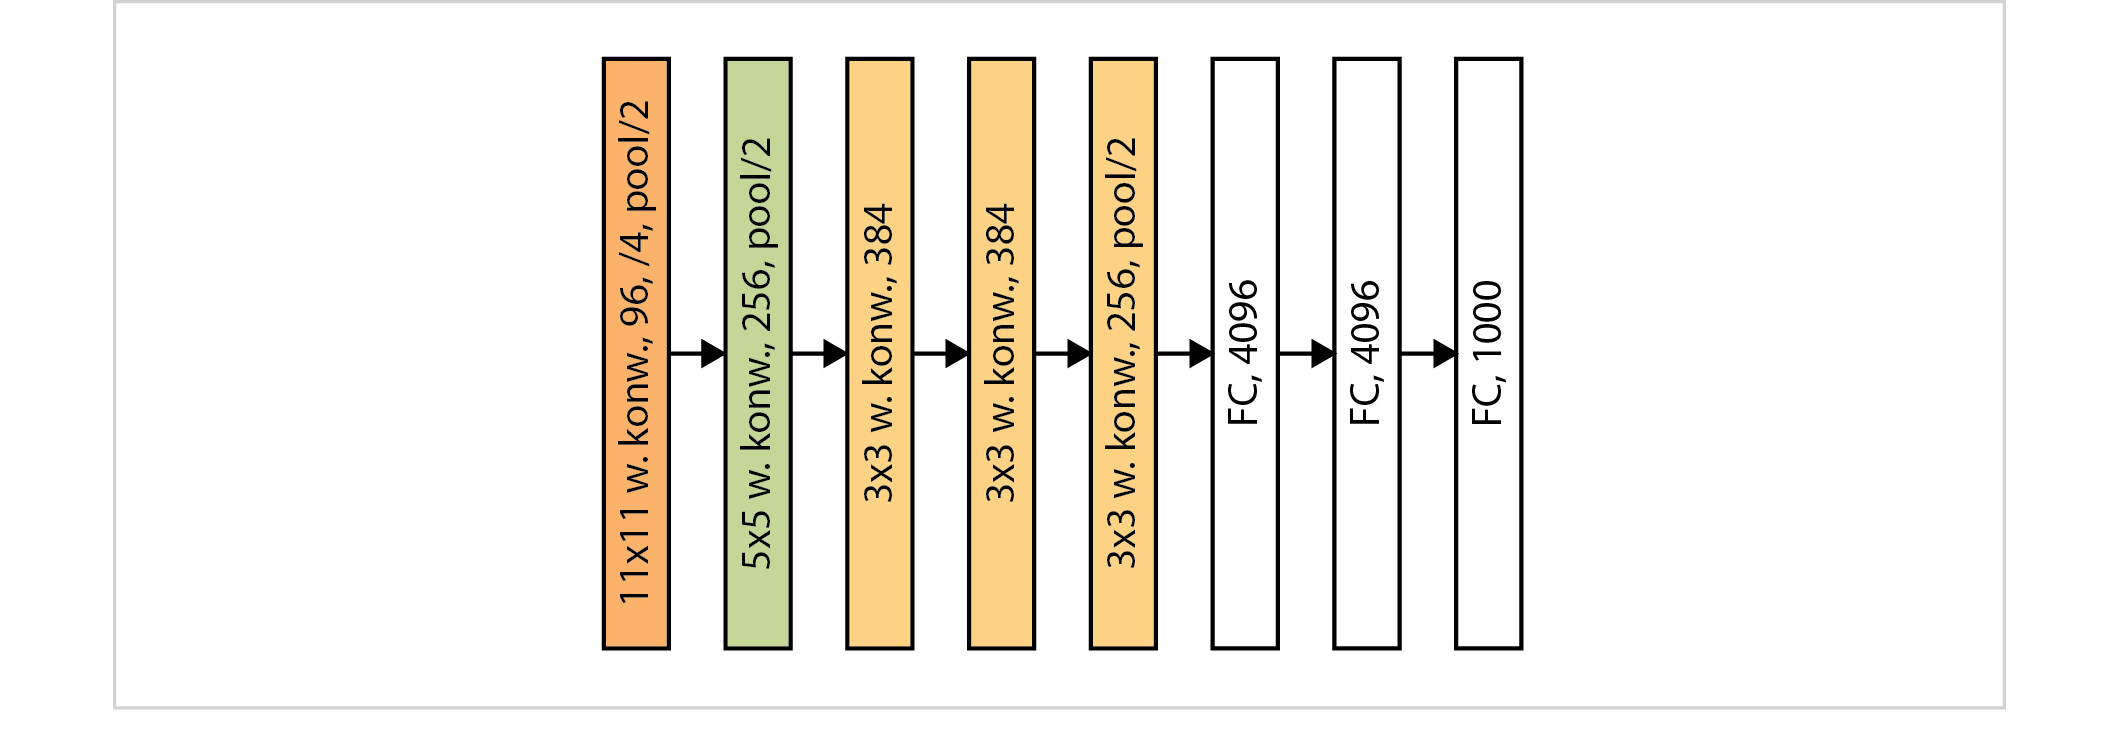
\includegraphics[width=1\textwidth]{figures/AlexNet.png}
	\caption{Schemat architektury AlexNet.}
	\label{AlexNetTopology}
\end{figure}

W skład topologii wchodzi pięć warstw konwolucyjnych i trzy gęste. Po pierwszej, drugiej i piątej warstwie konwolucyjnej występują operacje typu max-pool z maską o wymiarach 2$\times$2 \footnote{Autorzy pracy podają też przykłady użycia masek o wymiarze 2$\times$3, które nakładają się w przestrzeni funkcji obrazowej. Nie znalazły one jednak miejsca w finalnej implementacji.}. 

Pierwsza warstwa konwolucyjna przyjmuje na wejściu dane o wymiarze 227$\times$227$\times$3\footnote{3 jest liczbą kanałów kodujących kolor obrazka.}, na których wykonywana jest operacja splotu z 96 filtrami z maską o wymiarach 11$\times$11$\times$3 i krokiem 4. W rezultacie (uwzględniając również operację max-pool) objętość wynikowa przekazywana do kolejnej warstwy ma wymiar 27$\times$27$\times$96. W drugiej warstwie konwolucyjnej wykonywana jest operacja splotu z 256 filtrami z maską o wymiarach 5$\times$5$\times$96. Wymiar objętości wynikowej zostaje ponownie zredukowany poprzez operacje max-pool do 13$\times$13$\times$256. Kolejne 3 warstwy konwolucyjne są połączone bezpośrednio ze sobą. Trzecia warstwa zawiera 384 filtry z maską o wymiarze 3$\times$3$\times$256, w skład czwartej wchodzą 384 filtry z maską o wymiarze 3$\times$3$\times$384, a w piątej znajduje się 256 filtrów również z maską o wymiarze 3$\times$3$\times$384. Końcowe dwie warstwy typu FC zawierają po 4096 neuronów, a ostatnia zawiera tyle neuronów ile klas występuje w ostatecznym podziale -- w oryginalnej pracy było to 1000 (por. \cite{Krizhevsky2012}).

Poniżej przedstawiono przykład algorytmu wykorzystywanego dla pierwszej warstwy konwolucyjnej opisywanej topologii, umożliwiający zrozumienie sposobu przetwarzania sygnału wejściowego: 
\begin{enumerate}
\item Z danych wejściowych o wymiarze [227$\times$227$\times$3] wybierany jest co czwarty blok  o wymiarach [11$\times$11$\times$3] (zarówno wzdłuż wysokości jak i szerokości). W rezultacie, nie uwzględniając krawędzi obrazu, otrzymywanych jest 217 punktów w każdym rzędzie i w kolumnie, w których mieści się [55$\times$55] tj. 3025 bloków.
\item Zarówno 11$\times$11$\times$3 = 363 wagi znajdujące się w 96 filtrach jak i wartości 363 punktów obrazowych znajdujących się 3025 blokach są przedstawiane w postaci macierzy $A$ o wymiarach [96$\times$363] i $B$ o wymiarach [363$\times$3025].
\item Liczony jest iloczyn skalarny w postaci A$^\intercal$B = $C$, gdzie nowa, wyjściowa macierz $C$ ma wymiar [96$\times$3025].
\item Rezultat w postaci macierzy $C$ ponownie przewymiarowany jest na postać [55$\times$55$\times$96].  
\end{enumerate} 

W architekturze jako funkcję aktywacji neuronów wykorzystano ReLU, co znacząco przyspieszyło trening sieci. Uzyskano 6-krotne przyspieszenie treningu dla danych CIFAR-10 (zob. \cite{CIFAR}) w stosunku do tej samej topologii wykorzystującej sigmoidalną funkcję aktywacji. Ponieważ funkcja ReLU nie posiada górnego ograniczenia, neurony teoretycznie mogą posiadać nieograniczone wartości funkcji aktywacji. W celu polepszenia kontrastu pomiędzy neuronami i wydobycia tych, które na tle innych się wyróżniają, zastosowano normalizację zgodną ze wzorem \ref{DLnormEquation}. W wyniku uzyskano redukcję błędu klasyfikacji top-5 o wartość 1,2 punktu procentowego.

W kontekście zwiększenia efektywności treningu zastosowano również powiększenie rozmiaru danych poprzez rotacje i modyfikacje funkcji obrazowej z wykorzystaniem czynników głównych (zob. \cite{Krizhevsky2012}) zmniejszając błąd top-1 o 1\%. Zastosowano też technikę dropout opisaną w \ref{sec-overffiting}. Ostatecznie wprowadzono także trening z wykorzystaniem wielu GPU (zob. Rys. \ref{AlexNetTopologyMultiGPU}). 

\begin{figure}[h!]
	\centering
	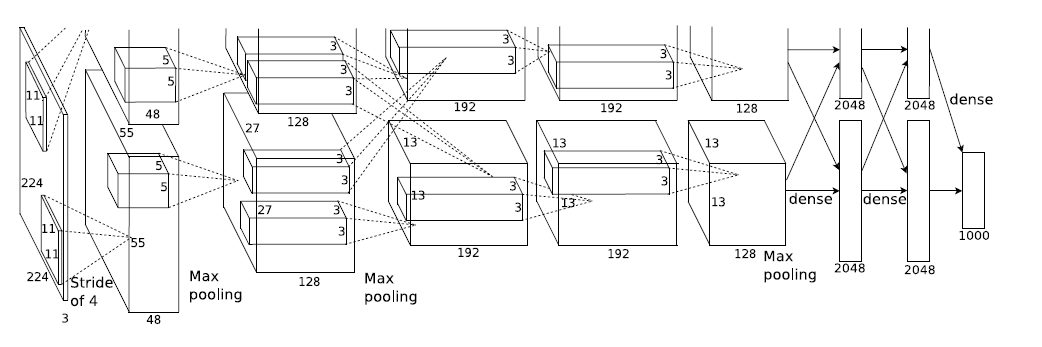
\includegraphics[width=1\textwidth]{figures/AlexNet-multiGPU.png}
	\caption{Topologia architektury AlexNet z podziałem na dwa akceleratory GPU.}
	\label{AlexNetTopologyMultiGPU}
\end{figure}

Topologia z podziałem na 2 karty zwiększyła dwukrotnie sumaryczną pamięć i pozwoliła na kolokację parametrów sieci.

Praca Alexa Krizhevsky, Ilya Sutskever i Geoffrey'a Hinton zapoczątkowała wzrost zainteresowania technikami głębokiego uczenia się, co doprowadziło do publikacji kolejnych podobnych architektur. Do najbardziej znanych należą ZFNet z 2013 roku \cite{ZFNet}, gdzie m.in. zastosowano zmniejszenie wymiaru maski stosowanego w filtrach pierwszej warstwy konwolucyjnej do 7$\times$7 oraz VGGNet \cite{VGGNet} z 2014 roku, gdzie zastosowano większą liczbę warstw konwolucyjnych z mniejszym wymiarem maski. Również w 2014 roku zaprezentowano innowacyjną koncepcję modułów sieci konwolucyjnych, co doprowadziło do zwycięstwa w ILSVRC. Idea ta została dokładniej opisana w kolejnej podsekcji.

\subsection{GoogLeNet}
\label{googlenet}
Architekturę o nazwie GoogLeNet zaprezentowano w 2014 r. w pracy \cite{GoogleNet}. Nazwa architektury pochodzi od nazwy zwycięskiego zespołu startującego w ILSVRC 2014, składającego się z pracowników firmy Google. Oryginalnie topologia składała się z 22 warstw i zawierała około 5 mln parametrów (12 razy mniej niż w przypadku sieci AlexNet). 

Redukcję liczby parametrów przy jednoczesnym podwyższeniu dokładności klasyfikacji obiektów udało się uzyskać poprzez poszukiwania konstrukcji optymalnych lokalnych topologii i ich połączeń. Mianowicie, wiadomo że duża część funkcji aktywacji neuronów przyjmuje wartość 0 lub jest redundantna z powodu wysokiej korelacji między sobą (zob. \cite{DBLP:journals/corr/AroraBGM13}). Matematyka dotycząca przetwarzania \textit{macierzy rzadkich}, tj. gdzie przeważająca liczba elementów przyjmuje wartość 0, jest dobrze znana (zob. np. \cite{Umit2010}). Jednak implementacje bibliotek do obliczeń związanych z algebrą liniową są zoptymalizowane pod kątem \textit{macierzy gęstych}, gdzie przeważająca liczba elementów przyjmuje wartości różne od 0 (zob. \cite{Song:2014:SUM:2597652.2597670, Krizhevsky2012}). 

Ideą modułu incepcji zaproponowanego przez twórców GoogLeNet jest aproksymacja rzadkich macierzy z użyciem komponentów o gęstej strukturze. Takie komponenty nazwano \textit{modułami incepcji} (ang. \textit{inception modules}), a ich przykłady pokazano na Rys. \ref{GoogleNetInceptionModules}. 
\begin{figure}[h!]
	\centering
	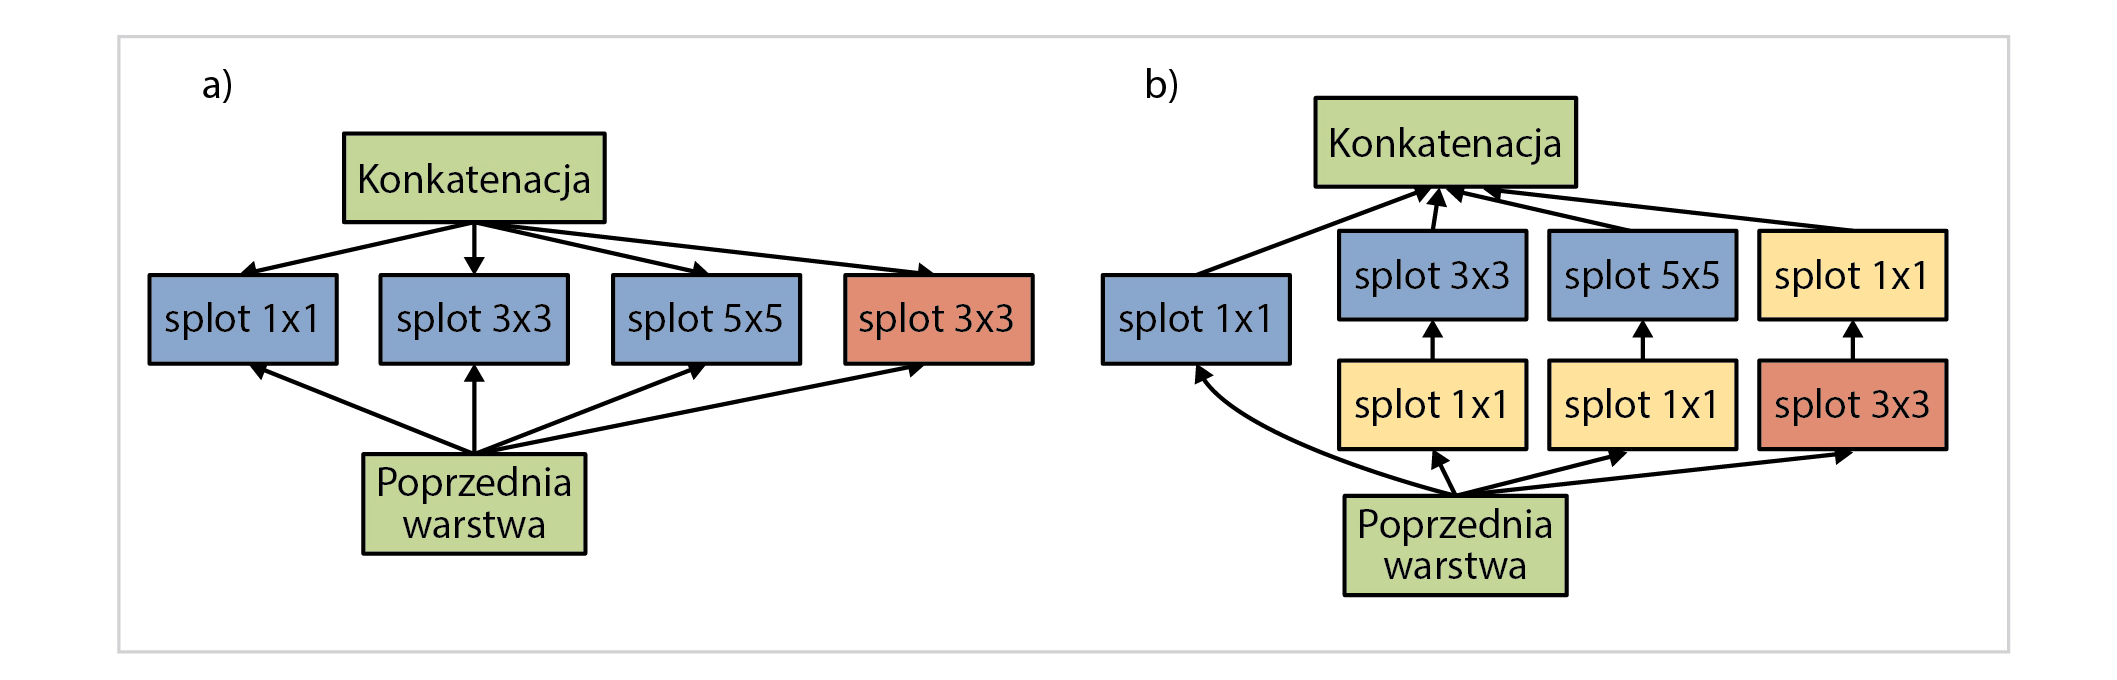
\includegraphics[width=1\textwidth]{figures/InceptionModules.png}
	\caption{Moduły incepcji o głębokości jednego (po lewej) i dwóch stopni (po prawej).}
	\label{GoogleNetInceptionModules}
\end{figure}

(a) przedstawia naiwną formę modułu incepcji, gdzie grupowane są operacje filtrów z maską o wymiarach 5$\times$5, 3$\times$3, 1$\times$1 oraz operacja max-pool. (b) prezentuje koncepcję zoptymalizowaną obliczeniowo gdzie filtry z maską 1$\times$1 służą do redukcji wymiarowości i używane są bezpośrednio przed splotami z bardziej wymagającymi obliczeniowo splotami 5$\times$5 i 3$\times$3. 

Przy pomocy złożenia różnego rodzaju modułów incepcji otrzymano topologię zaprezentowaną na Rys. \ref{GoogleNetTopo}.
\begin{figure}[h!]
	\centering
	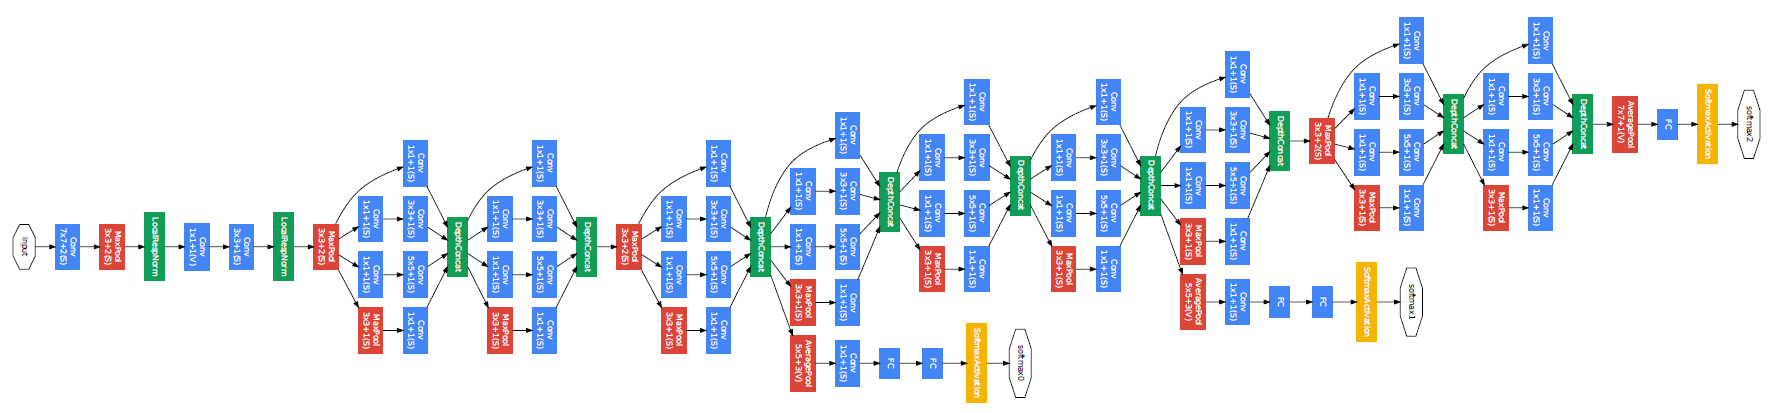
\includegraphics[width=1\textwidth]{figures/GoogleNet.png}
	\caption{Topologia architektury GoogleNet}
	\label{GoogleNetTopo}
\end{figure}
Zestawienie jej parametrów znajduje się w Tabeli \ref{GoogleNetParams}.
\renewcommand{\arraystretch}{1.2}
\begin{table}[h!]
	\setlength{\tabcolsep}{14pt}
	\centering
	\caption{Parametry architektury GoogleNet}
	\scriptsize
	\label{tab:USG-params}
	\begin{tabular}{l | c | c | c | c }
		%\hline
		Typ warstwy  & Wymiar  & Wymiar & Głębokość & Liczba   \\  
		& maski/krok & wyjściowy &&parametrów\\
	    \hline \hline
		Konwolucyjna   & 7$\times$7/2 & 112$\times$112$\times$64 & 1 & 2,7K \\ \hline
		Max-pool & 3$\times$3/2 & 56$\times$56$\times$64 & 0 & --  \\ \hline
		Konwolucyjna & 3$\times$3/2 & 56$\times$56$\times$192 & 2 & 112K  \\ \hline
		Max-pool & 3$\times$3/2 & 28$\times$28$\times$192 & 0 & --  \\ \hline
		M. incepcji & -- & 28$\times$28$\times$256 & 2 & 159K  \\ \hline
		M. incepcji & -- & 28$\times$28$\times$480 & 2 & 380K  \\ \hline
		Max-pool & 3$\times$3/2 & 14$\times$14$\times$480 & 0 & --  \\ \hline
		M. incepcji & -- & 14$\times$14$\times$512 & 2 & 364K  \\ \hline
		M. incepcji & -- & 14$\times$14$\times$512 & 2 & 437K  \\ \hline
		M. incepcji & -- & 14$\times$14$\times$512 & 2 & 463K  \\ \hline
		M. incepcji & -- & 14$\times$14$\times$528 & 2 & 580K  \\ \hline
		M. incepcji & -- & 14$\times$14$\times$832 & 2 & 840K  \\ \hline
		Max-pool & 3$\times$3/2 & 7$\times$7$\times$832 & 0 & --  \\ \hline
		M. incepcji & -- & 7$\times$7$\times$832 & 2 & 1072K  \\ \hline
		M. incepcji & -- & 7$\times$7$\times$1024 & 2 & 1388K  \\ \hline
		Avg-pool & 7$\times$7/2 & 1$\times$1$\times$1024 & 0 & --  \\ \hline
		Dropout (40\%) & -- & 1$\times$1$\times$1024 & 0 & --  \\ \hline
		Warstwa aktywacji & -- & 1$\times$1$\times$1000 & 1 & 1000K  \\ \hline
	\end{tabular}
	\label{GoogleNetParams}
\end{table}
\renewcommand{\arraystretch}{1}
Ważną cechą sieci GoogleNet jest brak warstw typu FC na zakończeniu, gdzie w przypadku sieci AlexNet znajduje się około 90\% parametrów. Końcowe wnioskowanie jest realizowane na podstawie wartości średniej z dwuwymiarowych map cech.

Dla lepszego zrozumienia idei redukcji wymiarowości realizowanej przez moduły incepcji, podobnie jak w przypadku sieci AlexNet, przeanalizowane zostanie działanie pierwszego modułu w topologii z Rys. \ref{GoogleNetTopo}.
Moduł zawiera 128 filtrów z maskami o wymiarach 3$\times$3 i 32 filtry z maskami o wymiarach 5$\times$5. Dane na wejściu modułu mają 192 kanały (zob. Tabela \ref{GoogleNetParams}). Dla przykładu, rząd wielkości obliczeń operacji splotów 32 filtrów 5$\times$5 wynosi 25$\times$32$\times$192=153 600 i dalej wzrastałby z głębokością sieci. W celu zapobiegnięcia nadmiarowi obliczeń stosowana jest redukcja z użyciem 16 filtrów z maską o wymiarach 1$\times$1. W efekcie rząd wielkości obliczeń spada do 16$\times$192 +  25$\times$32$\times$16=15 876, co pozwala na dalsze budowanie wielowarstwowych struktur.

Topologia GoogLeNet jest wciąż rozwijana. Po pierwszej prezentacji pojawiły się kolejne modernizacje wprowadzające dodatkowe faktoryzacje modułów jak w Inception-v2 lub normalizacje wartości wynikowych poszczególnych warstw jak w Inception-v3. Obie sieci zostały przedstawione w \cite{DBLP:journals/corr/SzegedyVISW15}. Kolejny innowacyjny pomysł, bazujący na dodatkowych połączeniach między blokami, został wprowadzony w 2015 roku w sieci ResNet opisanej w kolejnej podsekcji.

\subsection{ResNet}
\label{resnet}
Jednym z najbardziej oczywistych pomysłów na polepszenie dokładności działania sieci neuronowych jest zwiększenie liczby warstw. Jednak wraz ze wzrostem liczby warstw, trening takich architektur z użyciem tradycyjnych metod gradientowych (takich jak algorytm wstecznej propagacji błędu) staje się mniej wydajny. Problem wynika z faktu, że zmiana wartości sygnału na wyjściu sieci w odpowiedzi na sygnał wejściowy jest mniejsza wraz ze wzrostem liczby warstw. W takiej sytuacji gradient wyliczany na podstawie sygnału będącego różnicą pomiędzy sygnałem wejściowym a wyjściowym może przyjmować wartości bliskie 0 uniemożliwiając dalszy postęp uczenia się. Problem zanikającego gradientu (ang. \textit{vanishing gradient problem}) rozwiązywany jest poprzez zastosowanie normalizacji oraz nieliniowych funkcji aktywacji. Dzięki tym mechanizmom algorytm treningu głębokich sieci neuronowych w większej liczbie przypadków zbiega do użytecznego minimum lokalnego. 

W momencie znalezienia takiego minimum dodanie kolejnych warstw i parametrów sieci jest redundantne, a nawet prowadzi do pogorszenia wyników treningu sieci. Zjawisko to nosi nazwę \textit{degradacji treningu} (ang. \textit{degradation problem}). Twórcy architektury ResNet, przedstawionej w \cite{ResNet}, zaproponowali rozwiązanie tego problemu poprzez implementację bloków rezydualnych (ang. \textit{Residuum Units}) zawierających dodatkowe, skrótowe połączenia (ang. \textit{skip conections}) pomiędzy wejściem a wyjściem bloków. Porównanie schematów funkcjonalnych nowych bloków i wcześniej istniejącego rozwiązania stosowanego np. w AlexNet zostało przedstawione na Rys. \ref{ResNetBlock}.
\begin{figure}[h!]
	\centering
	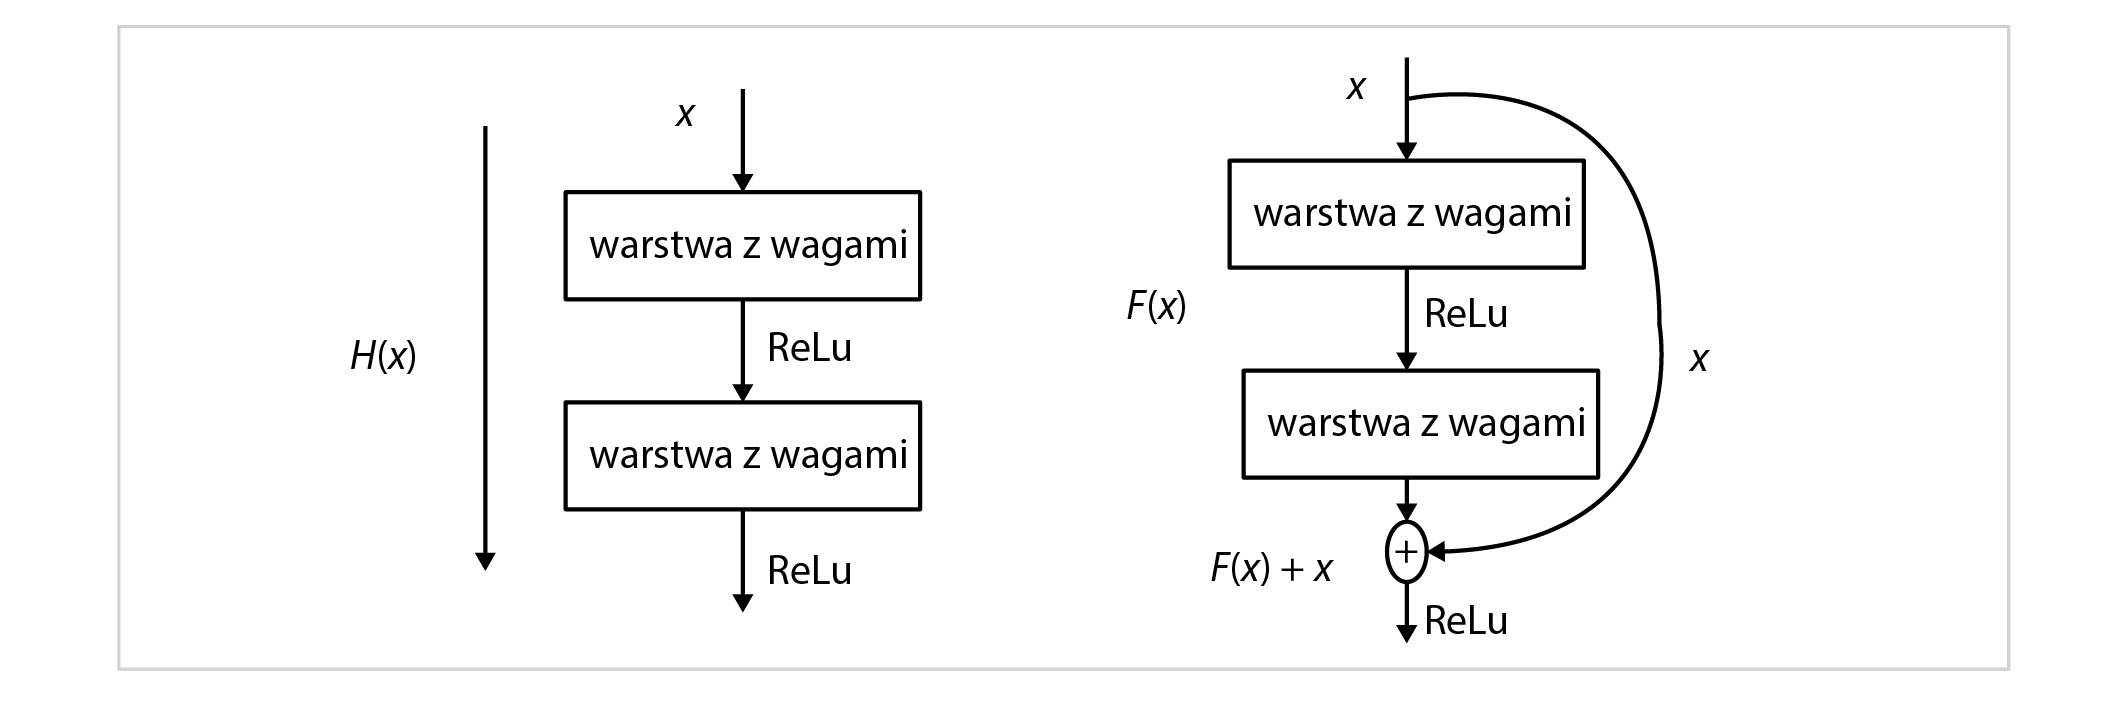
\includegraphics[width=1\textwidth]{figures/ResidualBlock.png}
	\caption{Schemat funkcjonalny pojedynczego bloku w architekturze ResNet.}
	\label{ResNetBlock}
\end{figure} 

Ogólną postać równania bloku rezydualnego można zapisać następująco:
\begin{equation}
\begin{split}
y_l = h(x_l) + F(x_l, W_l),\\
x_{l+1} = f(y_l),
\end{split}
\end{equation}
gdzie $x_l$ i $x_{l+1}$ stanowią sygnał wejściowy i wyjściowy $l$-tego bloku. $F$ stanowi funkcję rezydualną optymalizowaną podczas treningu sieci, $h$($x_l$) stanowi funkcję przekształcenia sygnału $x_l$ przekazywanego skrótowym połączeniem, $f$ jest funkcją ReLU, a $W$ stanowi macierz wag.

Funkcja $h$($x_l$) jest funkcją tożsamościową, a zatem $h$($x_l$) = $x_l$. Żeby uzasadnić ten wybór należy rozważyć propagację gradientu wewnątrz sieci składającej się z bloków rezydualnych. Dla każdego $L$-tego bloku zachodzi równanie:
\begin{equation}
x_L = x_l + \sum_{i=l}^{L-1}F(x_i, W_i)
\end{equation}
Korzystając z reguły łańcuchowej można zapisać równanie na gradient funkcji kosztu $\varepsilon$:
\begin{equation}
\label{gradResBlock}
\frac{\partial \varepsilon}{\partial x} =  \frac{\partial \varepsilon}{\partial x_L} \frac{\partial x_L}{\partial x_l} =  \frac{\partial \varepsilon}{\partial x_L}\left (1 +   \frac{\partial }{\partial x_l}\sum_{i=l}^{L-1}F(x_i, W_i) \right )
\end{equation}
z czego wynika, że gradient może być podzielony na dwie addytywne składowe: (1) $w$ = $\frac{\partial \varepsilon}{\partial x_L}$ propagowaną bez wpływu na warstwy zawierające wagi i (2) $\lambda$ = $\frac{\partial \varepsilon}{\partial x_L}\frac{\partial }{\partial x_l}\sum_{i=l}^{L-1}F(x_i, W_i)$ propagowaną przez nie.

Przykład propagacji gradientu w sieci składającej się z trzech bloków wygląda zatem następująco:
\begin{equation}
\label{gradRes3Block}
\frac{\partial \varepsilon}{\partial x_0} =  \frac{\partial \varepsilon}{\partial x_3}*(w_2+\lambda_2)*(w_1+\lambda_1)*(w_0+\lambda_0)
\end{equation}

Wartości $w$ są zazwyczaj znormalizowane do przedziału (-1;1) można więc rozważyć 4 istotne przypadki równania \ref{gradRes3Block}:
\begin{enumerate}
	\item $\lambda$ = 0 -- nie ma skrótowych połączeń, co odpowiada płaskiej strukturze sieci. Ponieważ wartości $w$ są z przedziału (-1;1) dodawanie kolejnych warstw wzmacnia wcześniej omówiony efekt zanikającego gradientu
	\item $\lambda$ $>$ 1 -- z każdą warstwą, sumaryczna wartość gradientu zwiększa się inkrementalni, co nazywane jest \textit{problemem eksplozji gradientu} (ang. \textit{exploding gradient problem}).
	\item $\lambda$ $<$ 1 -- przy założeniu, że $w$ + $\lambda$ $<$ 1, dla sieci składających się z wielu warstw występuje problem zaniku gradientu, jak w przypadku 1. Natomiast, gdy $w$ + $\lambda$ $>$ 1 podobnie jak w przypadku 2 może występować problem eksplozji gradientu
	\item $\lambda$ $=$ 1 -- wartości $w$ są inkrementowane dokładnie o 1, co eliminuje problemy podane w przypadkach 1, 2 i 3 i stanowi uzasadnienie dla wyboru funkcji tożsamościowej $h$($x_l$) w architekturze ResNet.
\end{enumerate}

Dokładny opis matematyczny funkcjonowania bloków rezydualnych wraz z dowodami znajduje się w \cite{DBLP:journals/corr/HeZR016}. Przykład topologii sieci składającej się z 8 bloków i łącznie 18 warstw tzw. ResNet-18, przedstawiono na Rys. \ref{ResNetTopo}.
\begin{figure}[h!]
	\centering
	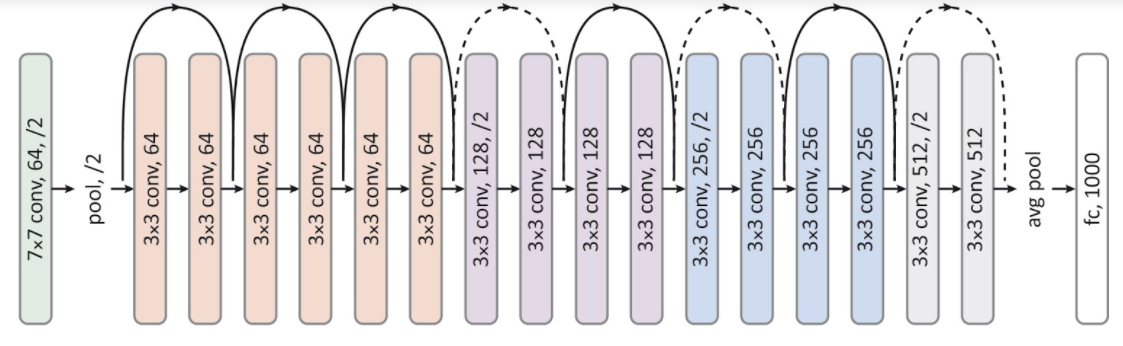
\includegraphics[width=1\textwidth]{figures/ResNet.png}
	\caption{Topologia architektury ResNet-18.}
	\label{ResNetTopo}
\end{figure} 

Pierwsza warstwa konwolucyjna zawiera filtry z maską o wymiarach 7$\times$7. W kolejnych zastosowano wymiar 3$\times$3. Zastosowanie mniejszych wymiarów masek niż w AlexNet oraz podobnie jak w przypadku sieci GoogLeNet wyliczenie na końcu wartości średniej z dwuwymiarowych map cech zredukowało liczbę parametrów.

Architektura ResNet-18 jest najmniejszą z pojawiających się w literaturze przykładów tego typu. W praktyce, z powodzeniem wykorzystywano topologie składające się nawet z 1202 warstw (zob. \cite{ResNet}). W 2016 roku zaprezentowano w \cite{InceptionResNet} hybrydę sieci GoogleNet i ResNet. Pracowano również nad bardziej złożonymi blokami, co w konsekwencji doprowadziło w 2017 roku do zaprezentowania architektury ResNetX w \cite{ResNetX}, która w wielu testach klasyfikacji różnych zbiorów okazała się być lepsza niż poprzednicy. Przegląd dotyczący historii tych prac można znaleźć w \cite{ResNetXoverview}.

Sieć ResNet i jej warianty dla wielu testowych zbiorów danych takich jak ImageNet, CIFAR czy COCO \cite{COCO} osiągnęły dokładność klasyfikacji porównywalną z możliwościami ludzkiego obserwatora. Dalszy progres był możliwy m.in. dzięki zastosowaniu synergii wielu modeli, co zostało opisane w kolejnej podsekcji.

\subsection{Złożenia}
Uczenie złożeń sieci (ang. \textit{esemble learning}) polega na wykorzystywaniu kilku modeli bazowych i wybranej metody ich synergii. W kontekście głębokiego uczenia się stosowane są różne metody kombinacji modeli bazowych (zob. \cite{Ensemble}). Jako często stosowane przykłady można podać: uśrednianie, głosowanie, klasyfikacja Bayesa, generalizację stosów. Zostaną one kolejno omówione:

\subsubsection{Uśrednianie}
Uśrednianie jest prostą metodą kombinacji wyników predykcji. Najczęściej stosowane jest uśrednienie bez wag, gdzie suma wyników predykcji modeli bazowych podzielona jest przez ich liczbę. Uśredniać można bezpośrednio wyniki ostatecznej klasyfikacji jak również prawdopodobieństwa przynależności do odpowiednich klas, które są np. wynikiem \textit{funkcji softmax}:
\begin{equation}
\sigma (z)_j= \frac{e^{z_j}}{\sum_{k=1}^{K} e^{z_k}},
\end{equation} 
używanej często bezpośrednio przed ostatnią warstwą sieci neuronowych dla $z$ sygnałów wejściowych i $j$ wyjściowych.

Główną zaletą uśredniania jest redukcja wariancji. Jest ona tym większa im bardziej nieskorelowane są wyniki predykcji modeli bazowych. Pomimo prostoty, tego rodzaju koncepcja odnosiła już sukcesy m.in. w lasach losowych (zob. \cite{Breiman2001}).

Zastosowanie uśredniania przy silnie odstających od średniej najgorszych predykcjach znacząco obniża dokładność całego złożenia. Dlatego przy tak nieheterogenicznych modelach bazowych dających bardzo różne wyniki poszukiwane są inne metody.

\subsubsection{Głosowanie}

W głosowaniu stosuje się mechanizm zliczania przewidzianych przez modele bazowe etykiet. Etykieta, która została wybrana przez największą liczbę modeli bazowych jest obierana jako wynik ostatecznej predykcji. Jest to tzw. \textit{głosowanie większościowe}.

W porównaniu do uśredniania, głosowanie jest mniej czułe na predykcje pojedynczych modeli. Wykorzystuje jednak jedynie informacje o przewidzianych etykietach, co utrudnia konstrukcje bardziej wyszukanych rozwiązań.

\subsubsection{Klasyfikacja Bayesa}

W przypadku tej metody, każdy model bazowy $j$ postrzegany jest jako hipoteza $h_j$. Każda z hipotez posiada wagę proporcjonalną do prawdopodobieństwa zdarzenia, w którym dany zbiór trenujący zostałby wybrany z ogółu danych gdyby dana hipoteza była prawdziwa. Jest to tzw. optymalna klasyfikacja Bayesa, którą można zapisać następującym równaniem:
\begin{equation}
y = arg max_{c_j \in C} \sum_{h_i \in H} P(c_j \mid h_i)P(T \mid h_i)P(h_i)
\end{equation}
gdzie $y$ to przewidziana etykieta, $C$ jest zbiorem wszystkich możliwych klas, $H$ to przestrzeń hipotez, a $T$ to zbiór danych trenujących.

W praktyce z uwagi na dużą złożoność obliczeniową nie stosuje się optymalnej klasyfikację Bayesa, a jedynie aproksymacje tej metody np.: BPA (od ang. \textit{Bayesian parameter averaging}) \cite{BPA}, BMA (od ang. \textit{Bayesian model averaging}) \cite{BMA}, czy też BMC (od ang. \textit{Bayesian model combination}) \cite{BMC}.

\subsubsection{Generalizacja stosów}
Idea generalizacji stosów oryginalnie została zaproponowana w \cite{Wolpert92stackedgeneralization}. Wykorzystana została koncepcja \textit{meta-uczenia}, a zatem konstrukcja nadrzędnego klasyfikatora, którego zadaniem jest wybór optymalnego wektora wag $a$ dla stosu $s$ predykcji dla danych $x$:
\begin{equation}
s(x) = \sum_{i=1}^{m}a_i s_i(x)
\end{equation}

W praktyce predykcje z modeli bazowych składowane są na stosie, a następnie klasyfikator nadrzędny wykorzystuje je jako dane do treningu poprawnych wartości $a$ wykorzystując jako odniesienie znane, poprawne etykiety.
 

\section{Zastosowania w medycynie}

W 1994 roku ukazała się pierwsza praca, która w praktyce wykorzystywała mechanizmy związane z głębokim uczeniem się do przetwarzania obrazów medycznych (zob. \cite{Zhang1994}). Użyte wówczas sieci nazywano sieciami typu \textit{shift-invariant}. Zastosowanie ich pozwoliło na eliminacje 55\% FP otrzymywanych przy wcześniejszych metodach stosowanych do detekcji skupisk mikro-zwapnień w mammografach. \textit{Shift-invariant} oznaczało, że przesunięcie obrazu wejściowego nie powodowało zmian w klasyfikacji, co jest istotną wartością dodaną, z uwagi na specyfikę implementacji toru akwizycji danych w praktyce radiologicznej.

Po roku 2012 nastąpił znaczący wzrost zainteresowania metodami głębokiego uczenia się w medycynie. Obrazuje to praca \cite{Litjens2017} z 2017 roku, w której przytoczono statystyki medycznych publikacji zawierających słowa kluczowe związane z deep learning. Wybrane dane przedstawiono na Rys. \ref{DL_CAD_stats}.
\begin{figure}[h!]
	\centering
	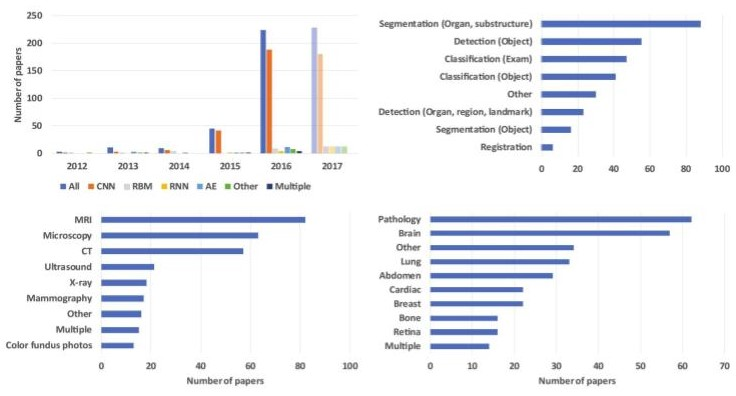
\includegraphics[width=1\textwidth]{figures/DL_CAD_statystyka.jpg}
	\caption{Statystyki dotyczące publikacji medycznych zawierających słowa kluczowe związane z głębokim uczeniem się.}
	\label{DL_CAD_stats}
\end{figure}

 Widoczny wzrost liczby publikacji nastąpił począwszy od 2015, co związane było z kilkuletnią adaptacją nowych metod w dziedzinie przetwarzania obrazów medycznych i gromadzeniem odpowiednich zbiorów danych. Lata 2016 i 2017 były pod pewnym względem przełomowe gdyż pojawiało się coraz więcej prac naukowych, w których przedstawiano rezultaty dokładności klasyfikacji na poziomie dorównującym ekspertom dziedzinowym.
 
 Dla przykładu, w Listopadzie 2016 ukazała się praca \cite{Gulshan2016} grupy Google Research z Mountain View w Kalifornii, gdzie zastosowano sieć GoogLeNet w wersji inception-v3 do zautomatyzowanej detekcji retinopatii cukrzycowej i cukrzycowego obrzęku plamki w obrazach dna oka. Wyniki porównano z panelem składającym się z 7 ekspertów, okulistów. Porównanie przedstawiono na Rys. \ref{CAD_opto}.
 \begin{figure}[h!]
 	\centering
 	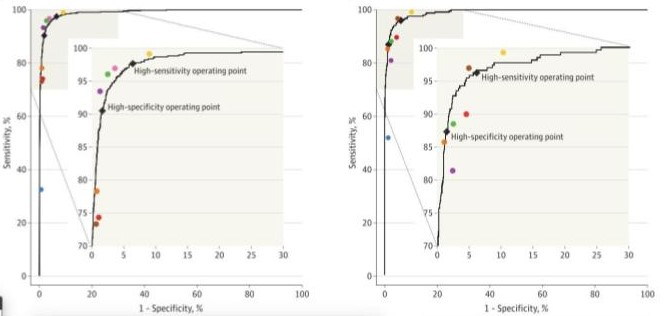
\includegraphics[width=0.7\textwidth]{figures/CAD-okulisci.jpg}
 	\caption{Porównanie automatycznej klasyfikacji retinopatii cukrzycowej i cukrzycowego obrzęku plamki z oceną panelu ekspertów.}
 	\label{CAD_opto}
 \end{figure}
 
 Na wykresach dla dwóch zadań klasyfikacyjnych umieszczono krzywe reprezentujące zależność swoistości od czułości dla algorytmu automatycznego oraz 7 punktów oznaczających wynik oceny każdego z okulistów. Ogółem mniej niż połowa ekspertów uzyskała lepszy wynik niż algorytm sztucznej inteligencji.
 
 Kolejna ciekawa praca tj. \cite{Esteva2017}, pojawiła się w czasopiśmie Nature w styczniu 2017 roku i traktowała o automatycznej detekcji nowotworów skóry na podstawie zdjęć. Autorzy wykorzystali dane składające się z 129.450 obrazów klinicznych, na których zobrazowano 2.032 różne schorzenia skóry. Ponownie do klasyfikacji wykorzystano sieć GoogleNet w wersji inception-v3. Wyniki klasyfikacji automatycznej porównano z oceną przeprowadzoną przez 21 certyfikowanych dermatologów. Przykład porównania zaprezentowano na Rys. \ref{CAD_derma}. 
 
 \begin{figure}[h!]
 	\centering
 	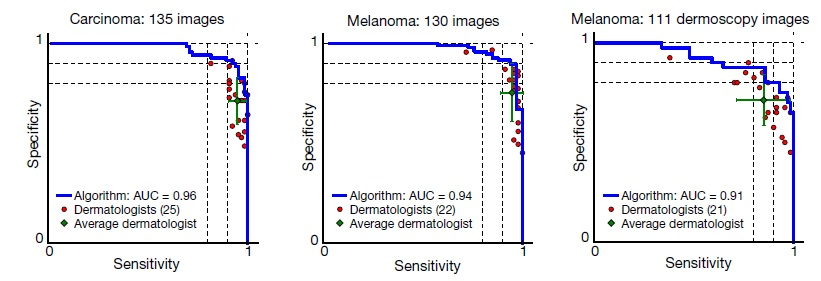
\includegraphics[width=0.9\textwidth]{figures/CAD-dermatolodzy.jpg}
 	\caption{Porównanie automatycznej klasyfikacji 3 chorób skóry z oceną ekspertów dermatologów.}
 	\label{CAD_derma}
 \end{figure}

Wykres przedstawia zależność czułości od swoistości. Czerwonymi punktami oznaczono wynik oceny poszczególnych ekspertów, a zielonym krzyżykiem wynik uśredniony. W każdym przypadku średnia ocena była gorsza od automatycznej klasyfikacji.

Obrazy medyczne nie są jedynymi danymi, które z powodzeniem są przetwarzane za pomocą metod głębokiego uczenia się. W lipcu 2017, przez grupę ze Stanford University została opublikowana praca \cite{2017arXiv170701836R} dotycząca klasyfikacji arytmii na podstawie szeregów czasowych zapisanych na elektrokardiogramach. Autorzy wykorzystali dane z 64.121 elektrokardiogramów, próbkowanych z częstotliwością 200 Hz, pochodzących od 29.163 pacjentów. Zaprojektowano dedykowaną, 34-warstwową sieć konwolucyjną do detekcji 12 różnych dysfunkcji pracy serca, pracy prawidłowej i szumów (łącznie 14 klas). Wyniki klasyfikacji porównano z oceną prowadzoną przez 3 kardiologów. Średnia dokładność z oceny automatycznej wyniosła 80\%, natomiast manualnej 72\%.

Podobnych przykładów zostało opublikowanych dużo więcej. Architektura AlexNet z sukcesem była użyta do detekcji polipów w kolonoskopii w \cite{Tajbakhsh2016}. Sieć ResNet sprawdziła się w badaniach zrealizowanych w \cite{Erickson2018} w Mayo Clinic Rotschester. Dotyczyły one radio-genomiki i rozróżnienia zmian w mózgu bez konieczności biopsji. Złożenia natomiast z sukcesem zaaplikowano w pracach dotyczących detekcji nowotworów płuc, gdzie modele bazowe analizowały różne skale problemu (zob. \cite{LungChalenge}). W wielu pracach dotyczących radiologii raportuje się dokładność klasyfikacji automatycznej znacząco przewyższające możliwości dziedzinowych ekspertów np. \cite{Christiansen2018, Sarraf2016, Glasser2016, 2016arXiv160605718W}.

Powyższe przykłady pokazują, że dla szczególnych przypadków pewien element pracy eksperta zajmującego się danymi medycznymi (np. radiologa) może być z sukcesem wspomagany (lub nawet zastąpiony) przez algorytmy głębokiego uczenia się. Fakt ten ma swoje odzwierciedlenie w liczbie nowych firm stosujących głębokie sieci neuronowe do wspomagania medycyny i uzyskujących certyfikację medyczną. Infografikę przedstawiającą dynamikę tych zmian zaprezentowano na Rys. \ref{fda_cert}.

\begin{figure}[h!]
	\centering
	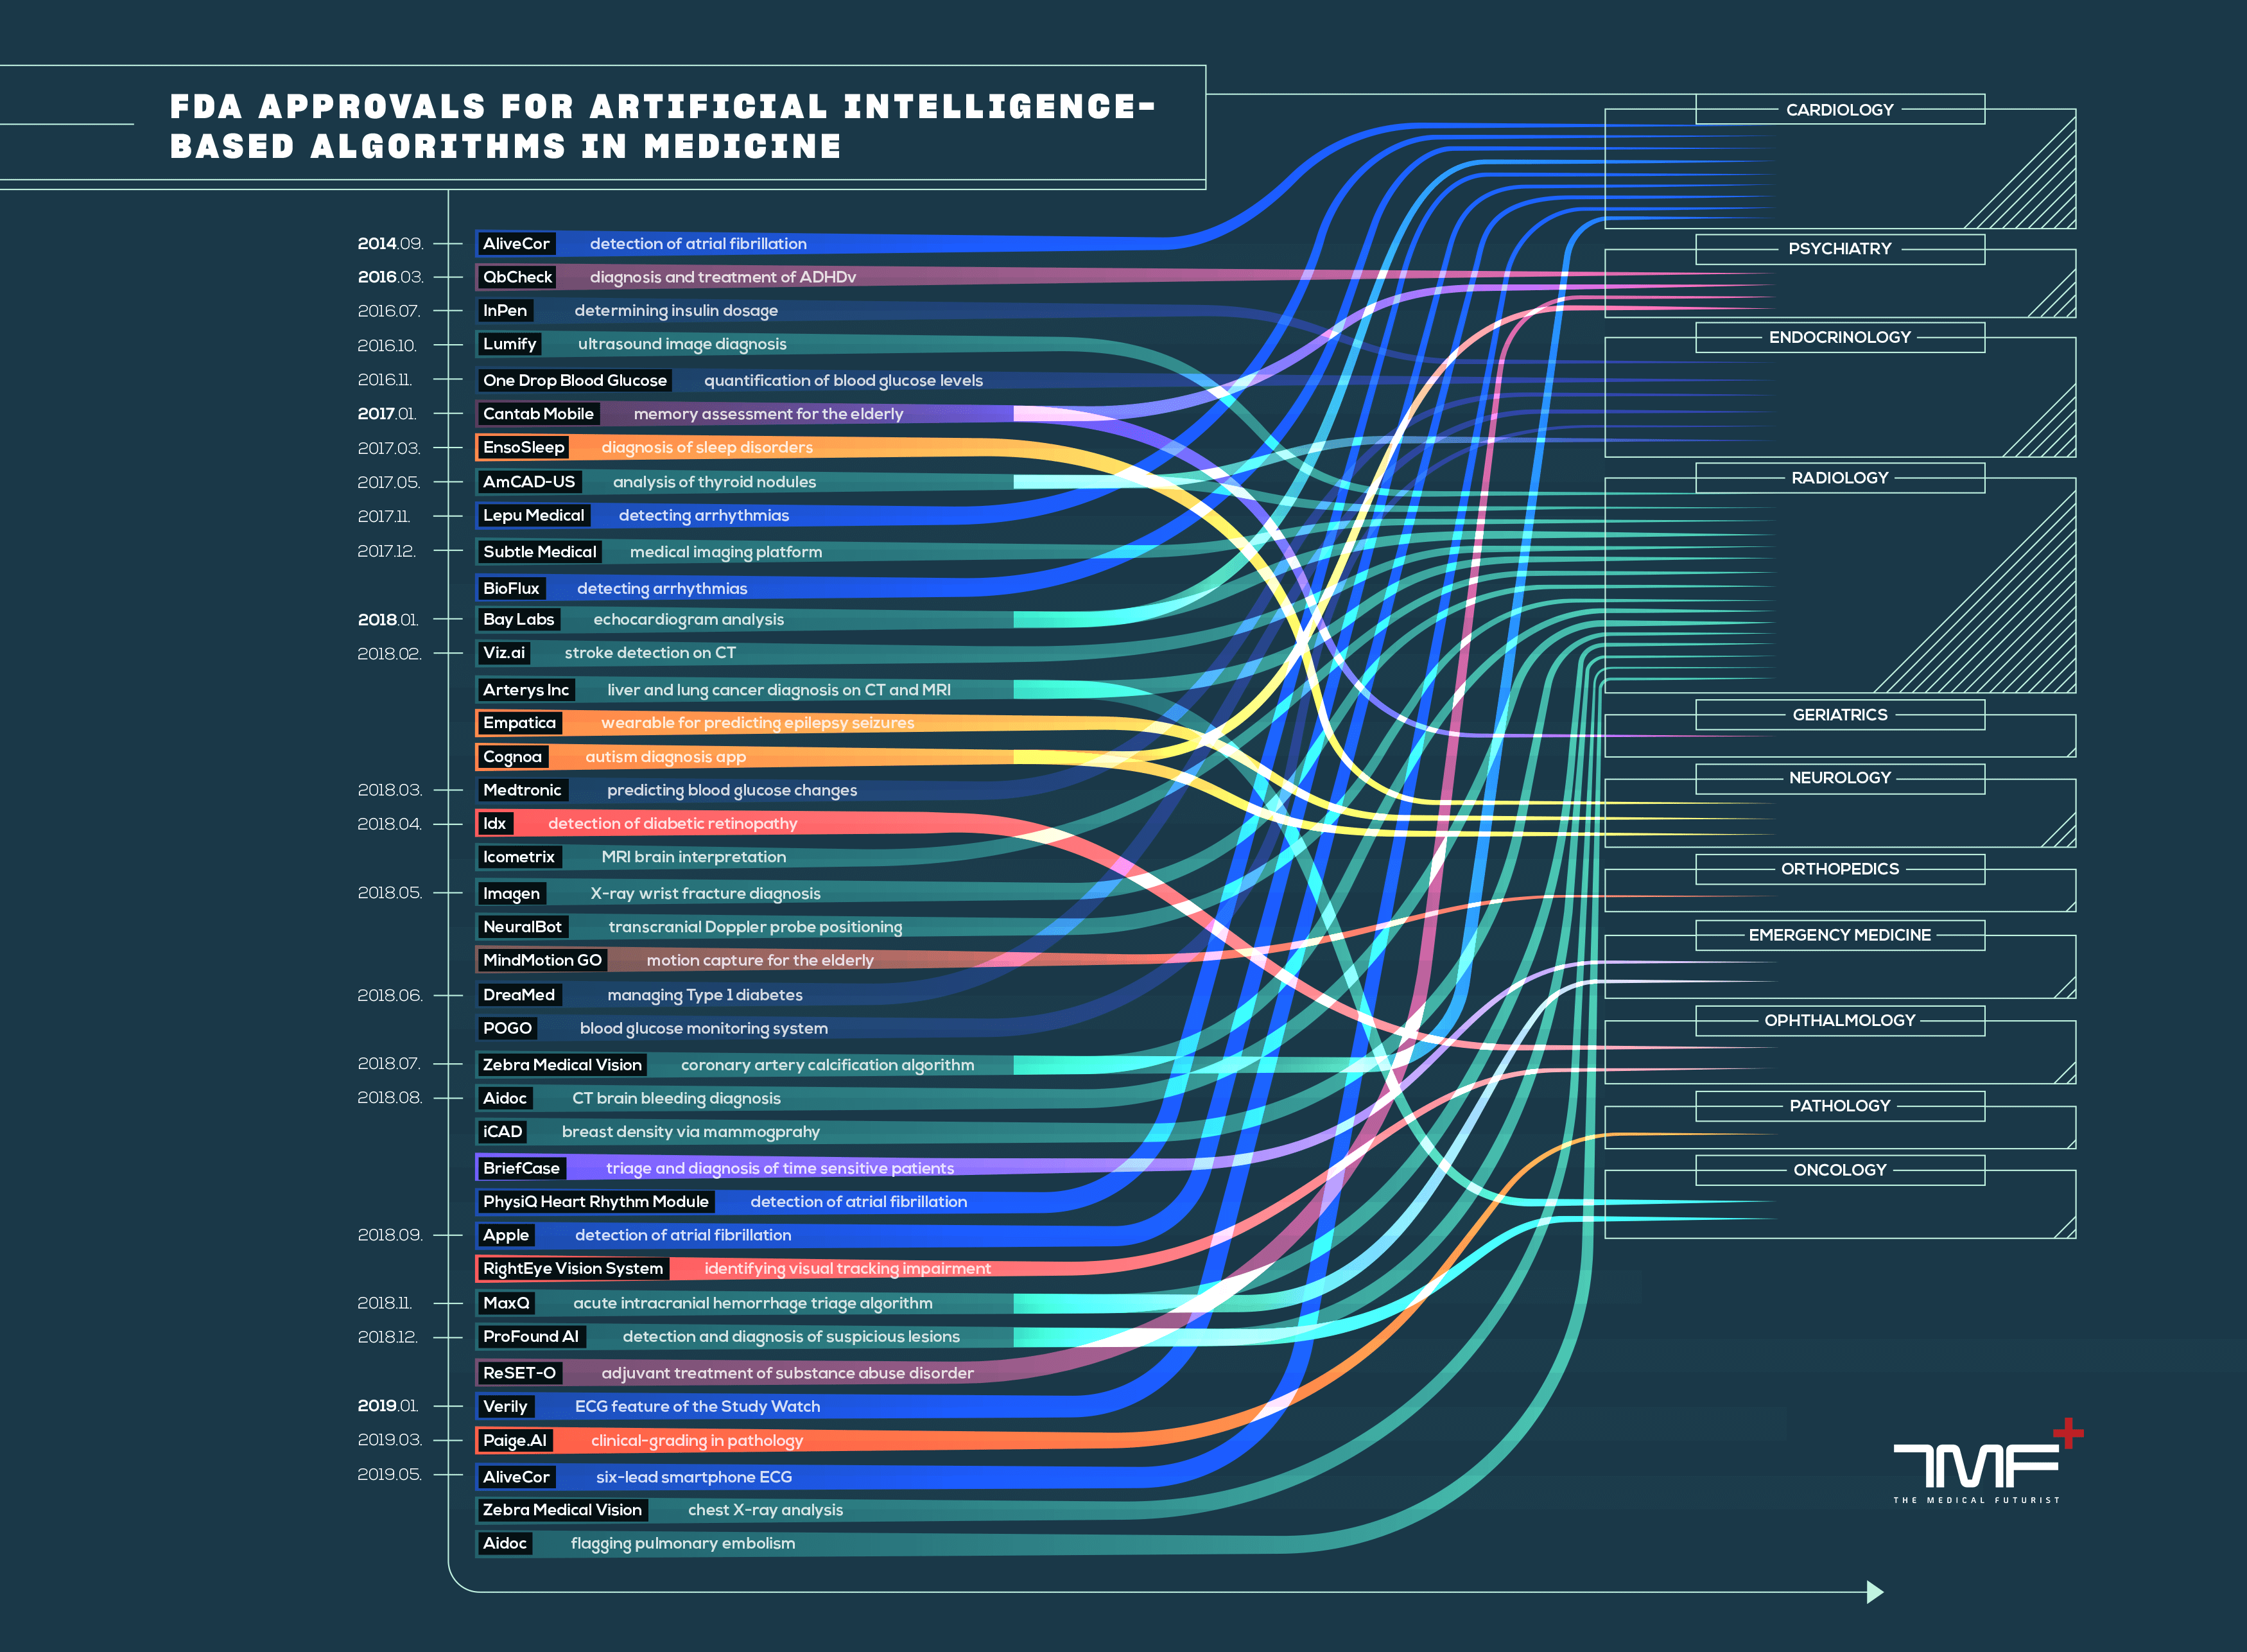
\includegraphics[width=0.9\textwidth]{figures/fda_for_ai.png}
	\caption{Firmy stosujące w swoich produktach głębokie sieci neuronowe, uzyskujące certyfikację FDA.}
	\label{fda_cert}
\end{figure}

Należy jednak podkreślić, że jest również szereg problemów wiążących się z wykorzystaniem tego rodzaju sztucznej inteligencji w medycynie. Do najważniejszych należą:
\begin{enumerate}
	\item Gromadzenie dużych zbiorów danych z odpowiednimi etykietami.
	\item Wykorzystanie heterogenicznych danych pochodzących np. z wielu urządzeń lub modalności.
	\item Kalibracja i szacowanie niepewności wyników modeli.
	\item Unifikacja modeli wykonujących podobne zadania.
	\item Minimalizacja liczby parametrów modelu przy zachowaniu satysfakcjonującego poziomu dokładności.
\end{enumerate}
Więcej na temat ograniczeń metod głębokiego uczenia się można przeczytać również w \cite{Marcus2018}.

Dyskusja dotycząca tych problemów wciąż jest tematem wielu paneli dyskusyjnych i debat konferencyjnych (zob np. \cite{NVIDIApanel}). Najbardziej zaawansowane prace dotyczą problemu gromadzenia dużych zbiorów danych medycznych, co wymaga bliskiej współpracy ekspertów medycznych z ekspertami od uczenia maszynowego. Często konieczna jest również modyfikacja bądź tworzenie dedykowanych programów do akwizycji danych medycznych. Jako przykłady takich inicjatyw można wymienić programy Stanford Medicine \cite{MedicalImageNet}, Harvard School of Medicine \cite{HMS} czy Massachusetts General Hospital, które w swoich repozytoriach zgromadziły już dziesiątki milionów zdjęć radiologicznych (za \cite{MGH}). Ponadto w roku 2018, na konferencji NVIDIA GTC (GPU Technology Conference) w San Jose (Kalifornia), Amerykańskie Stowarzyszenie Radiologii i stowarzyszenie MICCAI (od ang. \textit{Medical Image Computing and Computer Assisted Intervention}) ogłosiły porozumienie, co do wspólnej współpracy mającej na celu eliminacje barier legislacyjnych związanych ze współpracą przy pozyskiwaniu danych i wykorzystania algorytmów uczenia maszynowego.

Autor tej rozprawy jest świadom ograniczeń jakie są związane z wykorzystaniem algorytmów głębokiego uczenia się. Jednocześnie jednak nowe metody i ostatnie sukcesy zastosowań współczesnych sztucznych sieci neuronowych w aplikacjach medycznych stanowią silną motywację do przeprowadzenia własnych badań z ich wykorzystaniem.


    

\chapter{Nowa metoda oceny procesu gojenia ścięgna Achillesa}
\label{NewMethod}

W tym rozdziale zostanie zaprezentowana nowa metoda oceny procesu gojenia się ścięgna Achillesa bazująca na badaniach obrazowych RM. W szczególności, przedstawiony zostanie ilościowy opis umożliwiający w zobiektywizowany sposób ocenę morfologii tkanek widocznych w obrazach RM oraz nowatorskie podejście do automatycznego wyliczania wskazanych w opisie parametrów. 

Wedle najlepszej wiedzy autora, w chwili pisania tej pracy, nie istnieje podejście umożliwiające zobiektywizowany i co ważniejsze, automatyczny sposób oceny badań obrazowych prezentujących gojące się ścięgno Achillesa. Fakt ten implikuje trudności z integracją wyników radiologicznych z innymi formami oceny np. ze skalami testów funkcjonalnych, takich jak ATRS, czy wynikami badań biomechanicznych. W rezultacie zmniejszona jest efektywność całego procesu oceny rehabilitacji. 

Autor tej pracy, podczas próby rozwiązania wskazanego problemu, skupił się \linebreak na dwóch aspektach. Pierwszym z nich jest jakość generowanej automatycznie oceny, drugim czas akwizycji danych. W pierwszym przypadku jakość oceny automatycznej porównana została z oceną doświadczonego radiologa. W drugim, prace skupiły się wokół wyboru praktycznego protokołu, który zapewnił możliwie krótki udział pacjenta w badaniu. Celem jest poszukiwanie optimum, w którym maksymalizowana jest jakość oceny, a minimalizowany czas niezbędny do wykonania koniecznych czynności, zarówno przez radiologa jak i pacjenta. Szczegóły realizacji tego zadania przedstawiono w trzech kolejnych sekcjach rozpoczynając od przyjętej metodyki, następnie opisując eksperymenty służące do doboru metod i ich parametryzacji, \linebreak a kończąc na walidacji rozwiązania poprzez porównanie z oceną eksperta radiologa.

\section{Metodyka}
\label{seq:method}
W tej sekcji została szczegółowo opisana proponowana metoda automatycznej oceny procesu gojenia się ścięgna Achillesa widocznego w badaniach obrazowych Rezonansu Magnetycznego. Dodatkowo scharakteryzowany został zbiór danych, który posłużył do opracowania rozwiązania, jak również ankieta walidacyjna stanowiąca wzorzec odniesienia dla przedstawionej metody. 

Autor tej pracy, w proponowanym podejściu, skorzystał z metod widzenia komputowego, a dokładniej z fuzji algorytmów sztucznej inteligencji i przetwarzania obrazów. W kontekście tej pracy, pierwsze znajdują swoje zastosowanie do ekstrakcji wektora cech dla danej reprezentacji obrazowej, drugie, pozwalają uwzględnić wiedzę dziedzinową w procesie numerycznej oceny.

W przypadku algorytmów sztucznej inteligencji zastosowano,  opisane w Rozdziale \ref{CNNs}, konwolucyjne sieci neuronowe, a dokładniej AlexNet, GoogLeNet (Inception-v3) i ResNet-18 (z osiemnastoma warstwami konwolucyjnymi). W pierwszej kolejności wykonano szkolenie podanych sieci dla problemu binarnej klasyfikacji tj. rozróżnienia obrazów chorego i zdrowego ścięgna. Następnie, część klasyfikująca została usunięta z topologii sieci, pozostawiając ekstraktor cech z parametrami zoptymalizowanymi pod kątem wydobycia istotnej informacji opisującej różnice między zdrową i chorą tkanką. Na tak otrzymanym wektorze przeprowadzono redukcję wymiarowości z wykorzystaniem metody PCA (zob. p. \ref{DimReduction}). W wyniku przeprowadzonych eksperymentów, ostatecznie zdecydowano się uwzględnić w końcowym rozwiązaniu 200 pierwszych czynników głównych.

W przypadku metod przetwarzania obrazów zastosowano obliczenia cech z wydzielonego przez specjalistę radiologa \textit{ROI} (od ang. \textit{Region of Interest}), tj. obszaru reprezentującego tkanki otoczone ościęgnem. Sumarycznie wyliczono 46 klasycznych cech obrazowych, w tym: pole powierzchni ROI, 9 cech opisujących statystykę wartości pikseli i 36 cech Haralicka opisujących teksturę (zob. \cite{Haralick1973}). W ramach statystyk scharakteryzowano: minimum, maksimum, średnią, odchylenie standardowe, skośność, kurtozę, 25-percentyl, medianę oraz 75-percentyl. Natomiast w ramach cech Haralicka: drugi moment kątowy, kontrast, korelację, wariancję, odwrotny moment różnicowy, sumę średnich, sumę wariancji, sumę entropii, entropię, różnicę wariancji i maksimum prawdopodobieństwa. Cechy Haralicka wyliczono dla 3 dystansów separacji \textit{d}=1, 5, 10. Powyższa selekcja została dokonana na podstawie prac zawartych w \cite{Nowosielski17}.  

Na zbiorze wyliczonych 246-ciu cech dokonano selekcji metodą LASSO (zob. pkt \ref{DimReduction}). W rezultacie, dla wszystkich ocenianych parametrów, uzyskano optymalne podzbiory o liczebności poniżej 20-tu cech ekstrahowanych zarówno z wykorzystaniem sieci konwolucyjnych jak i klasycznych metod obrazowych. Predyktory \linebreak te posłużyły do szkolenia algorytmu meta-regresji, przy użyciu którego wykonana została fuzja prowadząca do końcowej oceny pacjenta realizowanego zaproponowaną przez autora tej pracy metryką $H$:
\begin{equation}
\label{ecq:H}
H = TM(R(x_1), R(x_2),..., R(x_n)),
\end{equation}
gdzie $TM$ jest średnią trymowaną z marginesami 2,5\%, a $R(x_i)$ jest wynikiem regresji obliczonym dla przekroju osiowego $x_i$, gdzie $i$ to indeks przekroju w trójwymiarowym badaniu RM.

Schemat proponowanej metody został zaprezentowany na Fig. \ref{fig:net}. 
\begin{figure}[h!]
	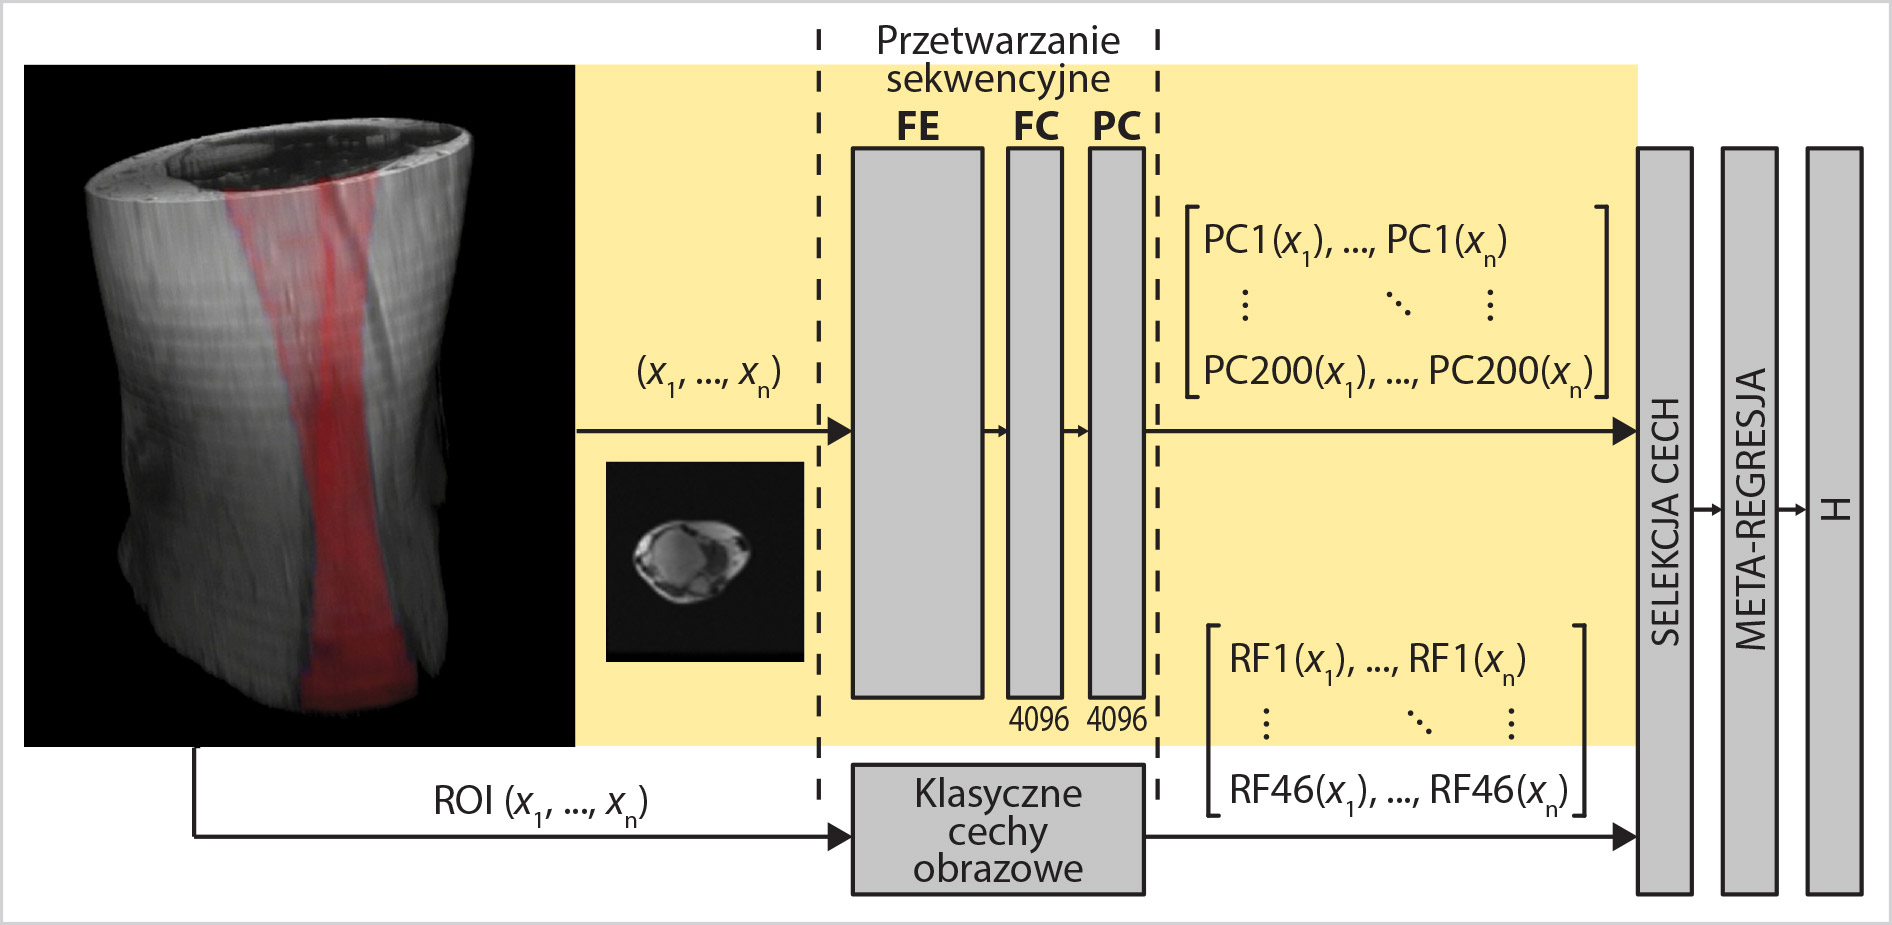
\includegraphics[width=\textwidth]{figures/net.jpg}
	\caption{Schemat automatycznej metody oceny procesu gojenia się ścięgna Achillesa.} \label{fig:net}
\end{figure}
W ogólnym ujęciu, trójwymiarowe badanie RM dzielone jest na pojedyncze przekroje osiowe, które stanowią dane wejściowe do oznaczonej na żółto części opartej o metody głębokiego uczenia się. W tym komponencie dane przetwarzane są przez ekstraktor cech sieci AlexNet (FE), którego parametry wybrano w wyniku eksperymentów. Otrzymane cechy wstępnie grupowane są z wykorzystaniem warstwy gęstej (FC) \linebreak i redukowane z 4096-ciu pojedynczych wyjść aktywacyjnych do 200 czynników głównych (PC).

Równolegle, ROI z każdego z przekrojów stanowi dane wejściowe do obliczeń klasycznych cech obrazowych. Końcowa fuzja realizowana jest z wykorzystaniem meta-regresji i metryki $H$. Takie podejście zapewnia numeryczny opis składający się z pojedynczej wartości dla całego badania RM.

\subsection{Zbiór danych}
\label{seq:zbior-danych}
Dane wykorzystane w tej pracy zostały zebrane w ramach projektu START "Wykorzystanie autologicznych mezenchymalnych komórek macierzystych w procesie regeneracji rekonstruowanego ścięgna Achillesa" finansowanego z konkursu STRATEGMED1 przez Narodowe Centrum Badań i Rozwoju. W ramach projektu, \linebreak do badanej grupy zakwalifikowano 60-ciu pacjentów po całkowitym zerwaniu ścięgna Achillesa i 29-ciu ochotników stanowiących grupę odniesienia. 

Kryteria wykluczające z grupy badanej zostały zdefiniowane tak, aby kwalifikowane osoby nie posiadały wcześniejszej historii urazów ścięgna Achillesa, ani przewlekłych chorób, które mogłyby spowodować degenerację tkanki ścięgnistej. Uwzględniono również warunki odbiegające od normy takie jak: otyłość, ciąża i infekcje. Ostatecznie, w ramach grupy pacjentów znalazło się 49 mężczyzn i 11 kobiet w wieku pomiędzy 24 a 49 lat, ze średnią 36 lat. Wszyscy pacjenci podpisali stosowne zgody wymagane do przeprowadzenia badań.   

52-óch z pośród 60-ciu pacjentów zerwało ścięgna podczas uprawiania sportu. Dokładniej były to: piłka nożna (19), squash/tenis (8), koszykówka (4), bieganie (3), podskoki (2), siatkówka (2) oraz badminton, box, piłka ręczna, fitness, cross-fit, skateboard, rugby i skakanka. Urazy w 31 przypadkach dotyczyły prawego ścięgna, \linebreak a w 29-ciu lewego. Średnia pozycja zerwania umiejscowiona była 57 mm ponad górnym konturem kości piętowej.

W okresie do tygodnia po urazie, pacjenci przeszli zabieg rekonstrukcji wykonany metodą szycia na otwartym ścięgnie (zob. p. \ref{gojenie}). Następnie rozpoczęto rehabilitację trwającą 12 miesięcy, monitorowaną z wykorzystaniem RM i USG. Wykonano również badania biomechaniczne w środkowym i końcowym okresie rehabilitacji, zgodnie z protokołem opisanym w p. \ref{biomechanika}.

Przy akwizycji danych z wykorzystaniem RM posłużono się aparatem GE Signa HDxt 1.5T wyposażonym w cewkę Foot \& Ankle dedykowaną do pomiarów w rejonie dolnej kończyny. Każde z badań RM było wykonane z użyciem 7 sekwencji i łącznie 10 modalności opisanych szczegółowo w p. \ref{RM}:
\begin{enumerate}[noitemsep,nolistsep]
	\item T1 zależne
	\item T2 zależne
	\item PD
	\item T2 mapping
	\item T2$^\ast$ GRE
	\item T2$^\ast$ GRE TE\_MIN
	\item 3D FSPGR
	\begin{itemize}
		\item In Phase Ideal
		\item Out Phase Ideal
		\item Fat Ideal
		\item Water Ideal 
	\end{itemize}
\end{enumerate}

W grupie zdrowych ochotników przeprowadzono pojedyncze badanie, natomiast pacjentów skanowano 10-krotnie w odpowiednio zdefiniowanych odstępach czasowych. Pierwsze badanie odbyło się przed operacją, a następnych 9 odpowiednio \linebreak w tygodniach: 1, 3, 6, 9, 12, 20, 26, 40 i 52 po operacji. W procesie zbierania danych wystąpiły problemy wynikające z braku obecności poszczególnych osób na badaniach lub z niespójności danych. Dlatego finalnie skompletowany zbiór składał się z homogenicznych badań 27 zdrowych ochotników (270 trójwymiarowych skanów RM, w skład których wchodziło wspomniane 10 modalności) oraz 59 badań pacjentów (5900 trójwymiarowych skanów RM z 10-oma modalnościami i 10-oma krokami czasowymi). Przykładowa wizualizacja danych pacjenta i osoby zdrowej znajduje się na Rys. \ref{fig:MRI_sample}. 
\begin{figure}[h!]
	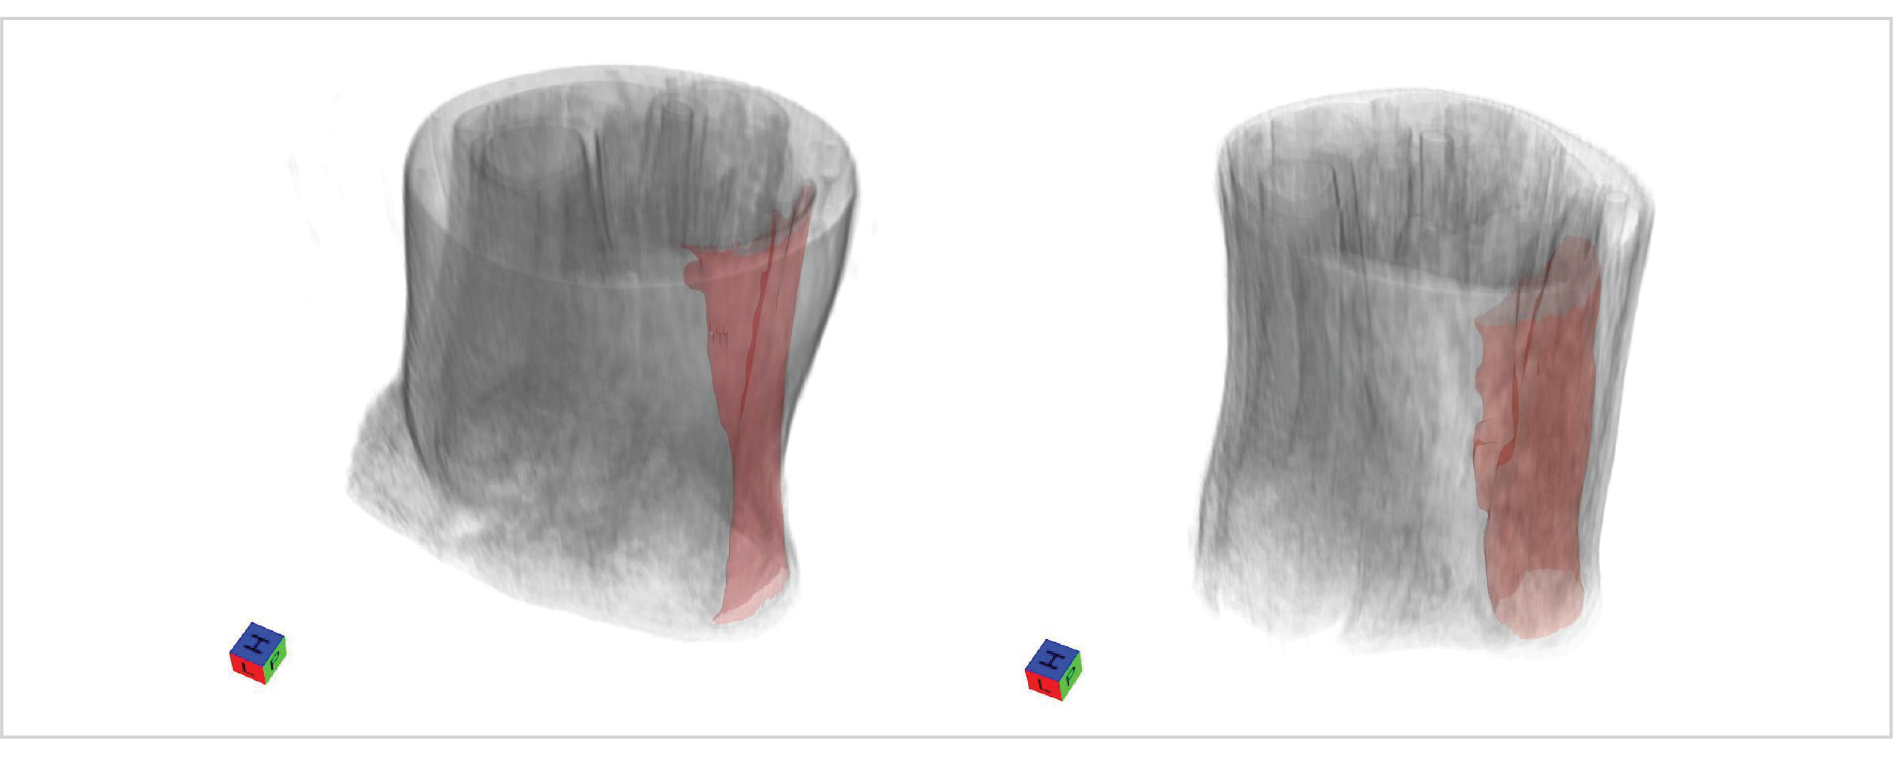
\includegraphics[width=\textwidth]{figures/Data_MRI_sample.jpg}
	\caption{Wizualizacja danych RM w sekwencji PD dla zdrowego (po lewej) i gojącego się (po prawej) ścięgna Achillesa.}
	 \label{fig:MRI_sample}
\end{figure}
Obszar zajmowany przez tkankę ścięgnistą został oznaczony na czerwono. Należy zwrócić uwagę na różnicę w kształcie, która dla zdrowego przykładu jest zgodna z opisem anatomicznym ujętym w p. \ref{anatomia}, natomiast dla przykładu chorego zawiera liczne deformacje. 

Spośród 59-ciu pacjentów zbadanych w ramach projektu START udało się zgromadzić ustrukturyzowany opis radiologiczny dla 48-miu z nich (480 badań). \linebreak W szczególności skompletowano ankietę opisaną w kolejnej podsekcji. Czterech pacjentów zostało losowo wydzielonych na początku eksperymentów jako pacjenci testowi, a pozostali stworzyli grupę pacjentów treningowych.

Zbiory trójwymiarowe posłużyły do opracowania zbiorów dwuwymiarowych składających się z przekrojów. W ten sposób udało się m.in. zwiększyć liczbę próbek wejściowych potrzebnych do szkolenia sieci neuronowych. Dane RM charakteryzują się wysoką anizotropią, a ich rozdzielczość wynosi 512$\times$512$\times$Z, gdzie $Z\in(10:50)$. Wyjątkiem jest sekwencja 3D FSPGR charakteryzująca się niższą anizotropią, jednak większą liczbą artefaktów wynikających z szybkiego czasu akwizycji. Zbiory oparte o RM zostały zatem opracowane w oparciu o przekroje osiowe 512$\times$512. Ważne jest również, że na każdym z tych przekrojów widoczne są elementy ścięgna Achillesa, co nie występuje w danych RM w przypadku przekrojów z pozostałych dwóch płaszczyzn.

Sumaryczna liczba tak uzyskanych próbek dwuwymiarowych wyniosła 11.725 (oznaczonych jako obrazy zdrowego ścięgna) i 138.604 (oznaczonych jako obrazy chorego ścięgna). W zależności od eksperymentów służących do optymalizacji parametrów metody wykorzystano:
\begin{itemize}[noitemsep,nolistsep]
	\item Powiększony zbiór treningowy RM -- zawierający przekroje osiowe ze wszystkich badań pacjentów treningowych, realizowanych wszystkimi sekwencjami. Liczba przekrojów w tym zbiorze została powiększona poprzez zastosowanie transformacji odbicia lustrzanego i, w przypadku chorych przykładów, 10-ciu obrotów w zakresie od -10 do 10 stopni. Finalnie, zbiór zawierał 234.502 przekrojów oznaczonych jako zdrowych i 277.208 oznaczonych jako chorych.
	\item Ograniczony zbiór treningowy RM -- zawierający przekroje osiowe ze zbioru 44-ech pacjentów treningowych jedynie w sekwencji T2$^\ast$ GRE TE\_MIN (18.863 próbek).
	\item Zbiór PCA -- wykorzystywany dalej w pracy do analiz PCA, zawierający próbki z powiększonego zbioru treningowego \linebreak ze wszystkich sekwencji RM dla 10-ciu losowo wybranych pacjentów (44.813).
\end{itemize}

W celu wnioskowania i porównań rezultatów metody posłużono się danymi \linebreak od 4-ech pacjentów testowych, z wykorzystaniem, w zależności od potrzeby, od 1 do 10 modalności RM. Szczegóły dotyczące poszczególnych wyborów znajdują się \linebreak w opisach eksperymentów.


\subsection{Wzorzec odniesienia}
\label{seq:ground-truth}
Do stworzenia wzorca odniesienia, w ramach projektu START, została powołana specjalna grupa robocza składająca się z eksperta radiologa, specjalistów ortopedów i ekspertów od komputerowo wspomaganej diagnostyki. Celem grupy było opracowanie opisu ilościowego odzwierciedlającego elementy, na podstawie których radiolog podejmuje subiektywną opinię. W wyniku prac stworzono zestaw sześciu parametrów oceniany w skali 0--7, opisujący proces gojenia się ścięgna Achillesa widoczny w obrazach RM:

\begin{enumerate}[noitemsep,nolistsep]
	\item Uszkodzenia śródścięgniste (SCT od ang. \textit{Structural Changes within the Tendon}) -- informuje o spójności włókien w obszarze ścięgna. Zawiera się w ROI. Ocena wykonywana zarówno w płaszczyźnie osiowej jak i strzałkowej\footnote{Wykorzystano oś skanowania, z uwagi na techniczne ograniczenia rezonansu -- zwłaszcza anizotropowość obrazów.}. 0 – całkowity brak uszkodzeń, 1 – bardzo małe uszkodzenia. 2 – małe uszkodzenia, 3 – uszkodzenia średniej wielkości , 4 – dość duże uszkodzenia. 5 – duże uszkodzenia, 6 - bardzo duże uszkodzenia, 7 - ekstremalnie duże uszkodzenia.
	\item Pogrubienie ścięgna (TT od ang. \textit{Tendon Thickening} -- najgrubsze miejsce (tj. najdłuższy wymiar) w kierunku strzałkowym widoczny na przekroju osiowym. Zawiera się w ROI. 0 – całkowity brak pogrubienia (3 mm--5 mm), 1 – bardzo małe pogrubienie (6 mm), 2 – małe pogrubienie (9 mm), 3 – średnie pogrubienie (12 mm), 4 –  dość duże pogrubienie (15 mm), 5 duże pogrubienie (18 mm), 6 – bardzo duże pogrubienie (21 mm), 7 – ekstremalnie duże pogrubienie (24 mm).
	\item Ostrość granic ścięgna/rozgraniczenie (STE od ang. \textit{Sharpness of the Tendon Edges}) -- informuje o jakości granicy między tkankami ścięgnistymi i otoczeniem, w szczególności czy brzeg jest fraktalny. Oceniane jest na zewnątrz ścięgna w płaszczyźnie osiowej. 0 – bardzo duża (idealna) ostrość, 1 – duża ostrość, 2 – dość duża ostrość, 3 – średnia ostrość, 4 – mała ostrość, 5 – bardzo mała ostrość, 6 – minimalna ostrość, 7 – całkowicie nieostre.
	\item Obrzęk ścięgna (TE od ang. \textit{Tendon Edema}) -- informuje o anomaliach \linebreak w gromadzeniu się płynów w obszarze ścięgna. Zawiera się w ROI i jest oceniany na przekrojach osiowych. 0 – całkowity brak obrzęku, 1 – bardzo mały obrzęk, 2 – mały obrzęk, 3 – obrzęk średniej wielkości, 4 – dość duży obrzęk, 5 – duży obrzęk, 6 – bardzo duży obrzęk, 7 -- ekstremalnie duży obrzęk.
	\item Jednorodność ścięgna (TU od ang. \textit{Tendon Uniformity}) -- informuje o prawidłowej teksturze poszczególnych przekrojów osiowych i podobieństwie sąsiednich przekrojów mierzonym w płaszczyźnie strzałkowej. Zawiera się w ROI. 0 – całkowity brak niejednorodności (jednorodne), 1 – bardzo małe niejednorodności, 2 – małe niejednorodności, 3 – niejednorodności średniej wielkości, 4 – dość duże niejednorodności, 5 – duże niejednorodności, 6 – bardzo duże niejednorodności, 7 –  ekstremalnie duże niejednorodności. 
	\item Obrzęk tkanek (TisE od ang. \textit{Tissue Edema}) -- informuje o powiększonym przedziale powięziowym ścięgna. 0  – całkowity brak obrzęku, 1 – bardzo mały obrzęk, 2 – mały obrzęk, 3 – obrzęk średniej wielkości, 4 – dość duży obrzęk, 5 – duży obrzęk. 6 – bardzo duży obrzęk, 7 -- ekstremalnie duży obrzęk.
\end{enumerate}

\section{Eksperymenty}
\label{seq:experiments}
W tej sekcji zaprezentowano eksperymenty mające na celu dobór poszczególnych komponentów i parametrów finalnej metody. W pierwszej kolejności zostało opisane badanie dotyczące szkolenia sieci neuronowych, celem wyboru ekstraktora cech dającego możliwość rozróżnienia ścięgien zdrowych od tych po zerwaniu (chorych). Następnie zaprezentowano badanie dotyczące obliczenia wektora cech na wyjściu sieci neuronowej i redukcji jego wymiarowości. W kolejnej części przedstawiono wybór sekwencji RM, stanowiących dane wejściowe do proponowanego w tej pracy algorytmu. Finalnie, w dwóch ostatnich podsekcjach, opisano dobór optymalnego zestawu cech ekstrahowanych z użyciem sieci neuronowej i klasycznych metod przetwarzania obrazów oraz fuzję z wykorzystaniem meta-regresji.  


\subsection{Rozróżnienie ścięgna zdrowego i po zerwaniu}
\label{binaryMRI}
W tym badaniu porównane zostały współczesne architektury sieci neuronowych w zadaniu klasyfikacji binarnej, rozróżniającej obrazy zdrowego od chorego ścięgna. W porównaniu uwzględniono topologie AlexNet (zob. p. \ref{AlexNet}), GoogLeNet Inception-v3 (zob. p. \ref{googlenet}) i ResNet-18 (zob. p. \ref{resnet}). W celu doboru hiperparametrów i optymalizacji parametrów sieci, zastosowano szkolenie z wykorzystaniem kroswalidacji z podziałem na 5 segmentów (zob. p. \ref{sec-overffiting}). W każdym z 5-ciu cykli, 3 segmenty były wykorzystane do treningu, 1 do walidacji i 1 do finalnych testów. Do celów tego badania wykorzystano powiększony zbiór treningowy RM. Wyniki zebrano w Tab. \ref{tab:binary-cross-validation}.
\vspace{10px}
\renewcommand{\arraystretch}{1.2}
\begin{table}[h!]
	\setlength{\tabcolsep}{14pt}
	\centering
	\caption{Wyniki szkolenia sieci neuronowych z wykorzystaniem kroswalidacji z podziałem na 5 segmentów, dla problemu klasyfikacji obrazów zdrowego i chorego ścięgna.}
	\label{tab:binary-cross-validation}
	\begin{tabular}{l | l | l | l | l }
		%\hline
		 & Średnia & Min   & Max   & $\sigma$   \\ \hline \hline
		AlexNet   & 99,19 & 99,15 & 99,24 & 0,04 \\ \hline
		ResNet-18 & 95,98 & 92,78 & 99,04 & 2,5  \\ \hline
		GoogleNet & 99,83 & 99,68 & 99,91 & 0,1  \\ \hline
	\end{tabular}
\end{table}
\renewcommand{\arraystretch}{1}

Dla wszystkich architektur, wyniki dokładności klasyfikacji najlepszych modeli osiągnęły wartość powyżej 99\%. Niemniej jednak, w przypadku architektury ResNet-18, najgorszy model klasyfikował z dokładnością 92,78\%, co przełożyło się również na najgorszy średni wynik równy 95,98\%. Fakt ten może wskazywać na tendencje \linebreak do nadmiernego dopasowywania się architektury ResNet-18. Niższa generalizacja modelu może wynikać z faktu tendencji tej architektury do ekstrakcji cech szczegółowych przez jądra splotu o wymiarze 3$\times$3 lub też niedoboru liczby danych wejściowych w odniesieniu do efektywnej optymalizacji wag splotu.

W kolejnym kroku, dla wszystkich trzech architektur, porównano czasy szkolenia przy zadanym problemie. Na Rys. \ref{fig:training_times} zestawiono łączny czas 5-iu iteracji procesu kroswalidacji.
\begin{figure}[h!]
	\includegraphics[width=\textwidth]{figures/TrainingtimesChart.jpg}
	\caption{Porównanie czasów treningu architektur na dwóch architekturach GPU: Pascal i Volta.}
	\label{fig:training_times}
\end{figure}
Porównano dwie architektury GPU, starszą Pascal P100 i nowszą Volta V100, zaprezentowaną w 2017 roku, charakteryzującą się udoskonalonym, osobnym układem optymalizowanym pod kątem operacji tensorowych realizowanych \linebreak w warstwach konwolucyjnych. Do szkolenia wykorzystano framework Caffe. Można zaobserwować, że wykorzystanie nowszej architektury GPU dało rezultaty około dwukrotnego przyspieszenia czasu szkolenia w przypadku AlexNet i ResNet oraz około 30\% w przypadku GoogLeNet. AlexNet zawiera najmniej warstw konwolucyjnych i optymalizowaną implementację klasyfikatora. Szkolenie tej architektury zajęło mniej niż jedną godzinę na GPU Volta. Dla porównania, sieci z bardziej skomplikowaną topologią tj. ResNet-18 i GoogLeNet, charakteryzują się odpowiednio czasami szkolenia w okolicach 20-stu i 48-miu godzin. 

Na podstawie zestawienia wyników dokładności klasyfikacji z czasami treningu można stwierdzić, że AlexNet i GoogleNet charakteryzują się większą generalizacją, a z tych dwóch modeli, czas szkolenia jest o blisko 47 godzin krótszy dla AlexNet. Dlatego właśnie ekstraktor cech tej architektury został wybrany do realizacji kolejnych eksperymentów. 

Należy również podkreślić, że istnieją sposoby na dalsze poprawienie wyników dokładności wnioskowania. Uzupełniające badanie dotyczące możliwości fuzji sieci AlexNet i ResNet-18 zostało opublikowane przez autora tej pracy w czasopiśmie Acta of Bioengineering and Biomechanics \cite{Kapinski19}. Wyniki mogą być również poprawione poprzez analizę lokalizacji przekrojów w przestrzeni trójwymiarowej, w szczególności poprzez uwzględnienie, że przekroje oddalone od miejsca zerwania bardziej przypominają tkanki zdrowe. Można zatem zastosować np. metody logiki rozmytej lub miękkiej klasyfikacji (zob. \cite{Liu2011}) w celu lepszego określenia przynależności próbek do klas. 

Powyższe podejścia w opinii autora tej pracy miałyby jednak sens tylko w przypadku uzyskania nowych danych, dla których proponowany algorytm uzyskiwałby gorsze rezultaty. Z uwagi na wysokie wyniki dokładności zaprezentowanego podejścia dla wykorzystywanego w tej pracy zbioru, na tym etapie badań autor nie zdecydował się na dalsze usprawnienia kosztem komplikacji algorytmu. Eliminacja wykrytych anomalii i wyników odosobnionych realizowana jest w tej pracy poprzez zastosowanie średniej trymowanej w zaproponowanej metryce $H$ (zob. wzór \ref{ecq:H}).

\subsection{Obliczanie i redukcja wymiarowości wektora cech}

Celem tego eksperymentu jest znalezienie zredukowanego wektora cech $w$ pochodzącego z wyjścia sieci neuronowej. W założeniu ma on zawierać możliwie dużo informacji z oryginalnego zbioru i minimalny wymiar. W tym celu, z oryginalnej architektury AlexNet została wydzielona część ekstraktora cech oraz pierwsza warstwa gęsta (zob. Rys. \ref{AlexNetTopology}). Zabieg ten umożliwił wstępne pogrupowanie cech obrazowych przy jednoczesnym braku ich dywersyfikacji w stopniu jaki robi to pełna sieć. Parametry ekstraktora cech przeniesiono z modelu wybranego w eksperymencie binarnej klasyfikacji. 

Wykorzystując Zbiór PCA (zob. \ref{seq:zbior-danych}) została przeprowadzona analiza czynników głównych (zob. p. \ref{DimReduction}), gdzie pojedynczą obserwację stanowił wektor 4096 aktywacji na wyjściu zmodyfikowanej architektury AlexNet. Porównanie poziomu wariancji zachowywanej przez różną liczbę czynników głównych zebrano w Tab. \ref{PCA-results}.
\vspace{10px}
\renewcommand{\arraystretch}{1.2}
\begin{table}[h!]
 \setlength{\tabcolsep}{12pt}
 \centering
 \caption{Rezultaty PCA dla 1, 10 i 200 pierwszych czynników głównych.}
 \label{PCA-results}
 \begin{tabular}{l|l|l|l}
 
 & PC1 & PC1--PC10 & PC1--PC200 \\ \hline \hline
 Udział wyjaśnionej wariancji & 50,2\% & 90,8\%   & 98,8\% \\ \hline 
 \end{tabular}
 \end{table}
\renewcommand{\arraystretch}{1}

Analiza umożliwiła redukcję wymiarowości i rozróżnienie między obserwacjami w poszczególnych krokach czasowych. Wyjścia po transformacji PCA nazywane \linebreak są dalej w pracy \textit{cechami DL}. Można zaobserwować, że 4096 wartości zredukowanych do jednej cechy DL zachowuje ponad 50\% poziomu wariancji. Odpowiednio 10 cech DL zapewnia poziom powyżej 90\%, a 200 poziom bliski 99\%. 

W kolejnym kroku zwizualizowano uśrednione wartości PC1 dla wyników wszystkich pacjentów ze zbioru PCA w kolejnych tygodniach rehabilitacji (zob. Rys. \ref{fig:H}).

\begin{figure}[h!]
	\centering
	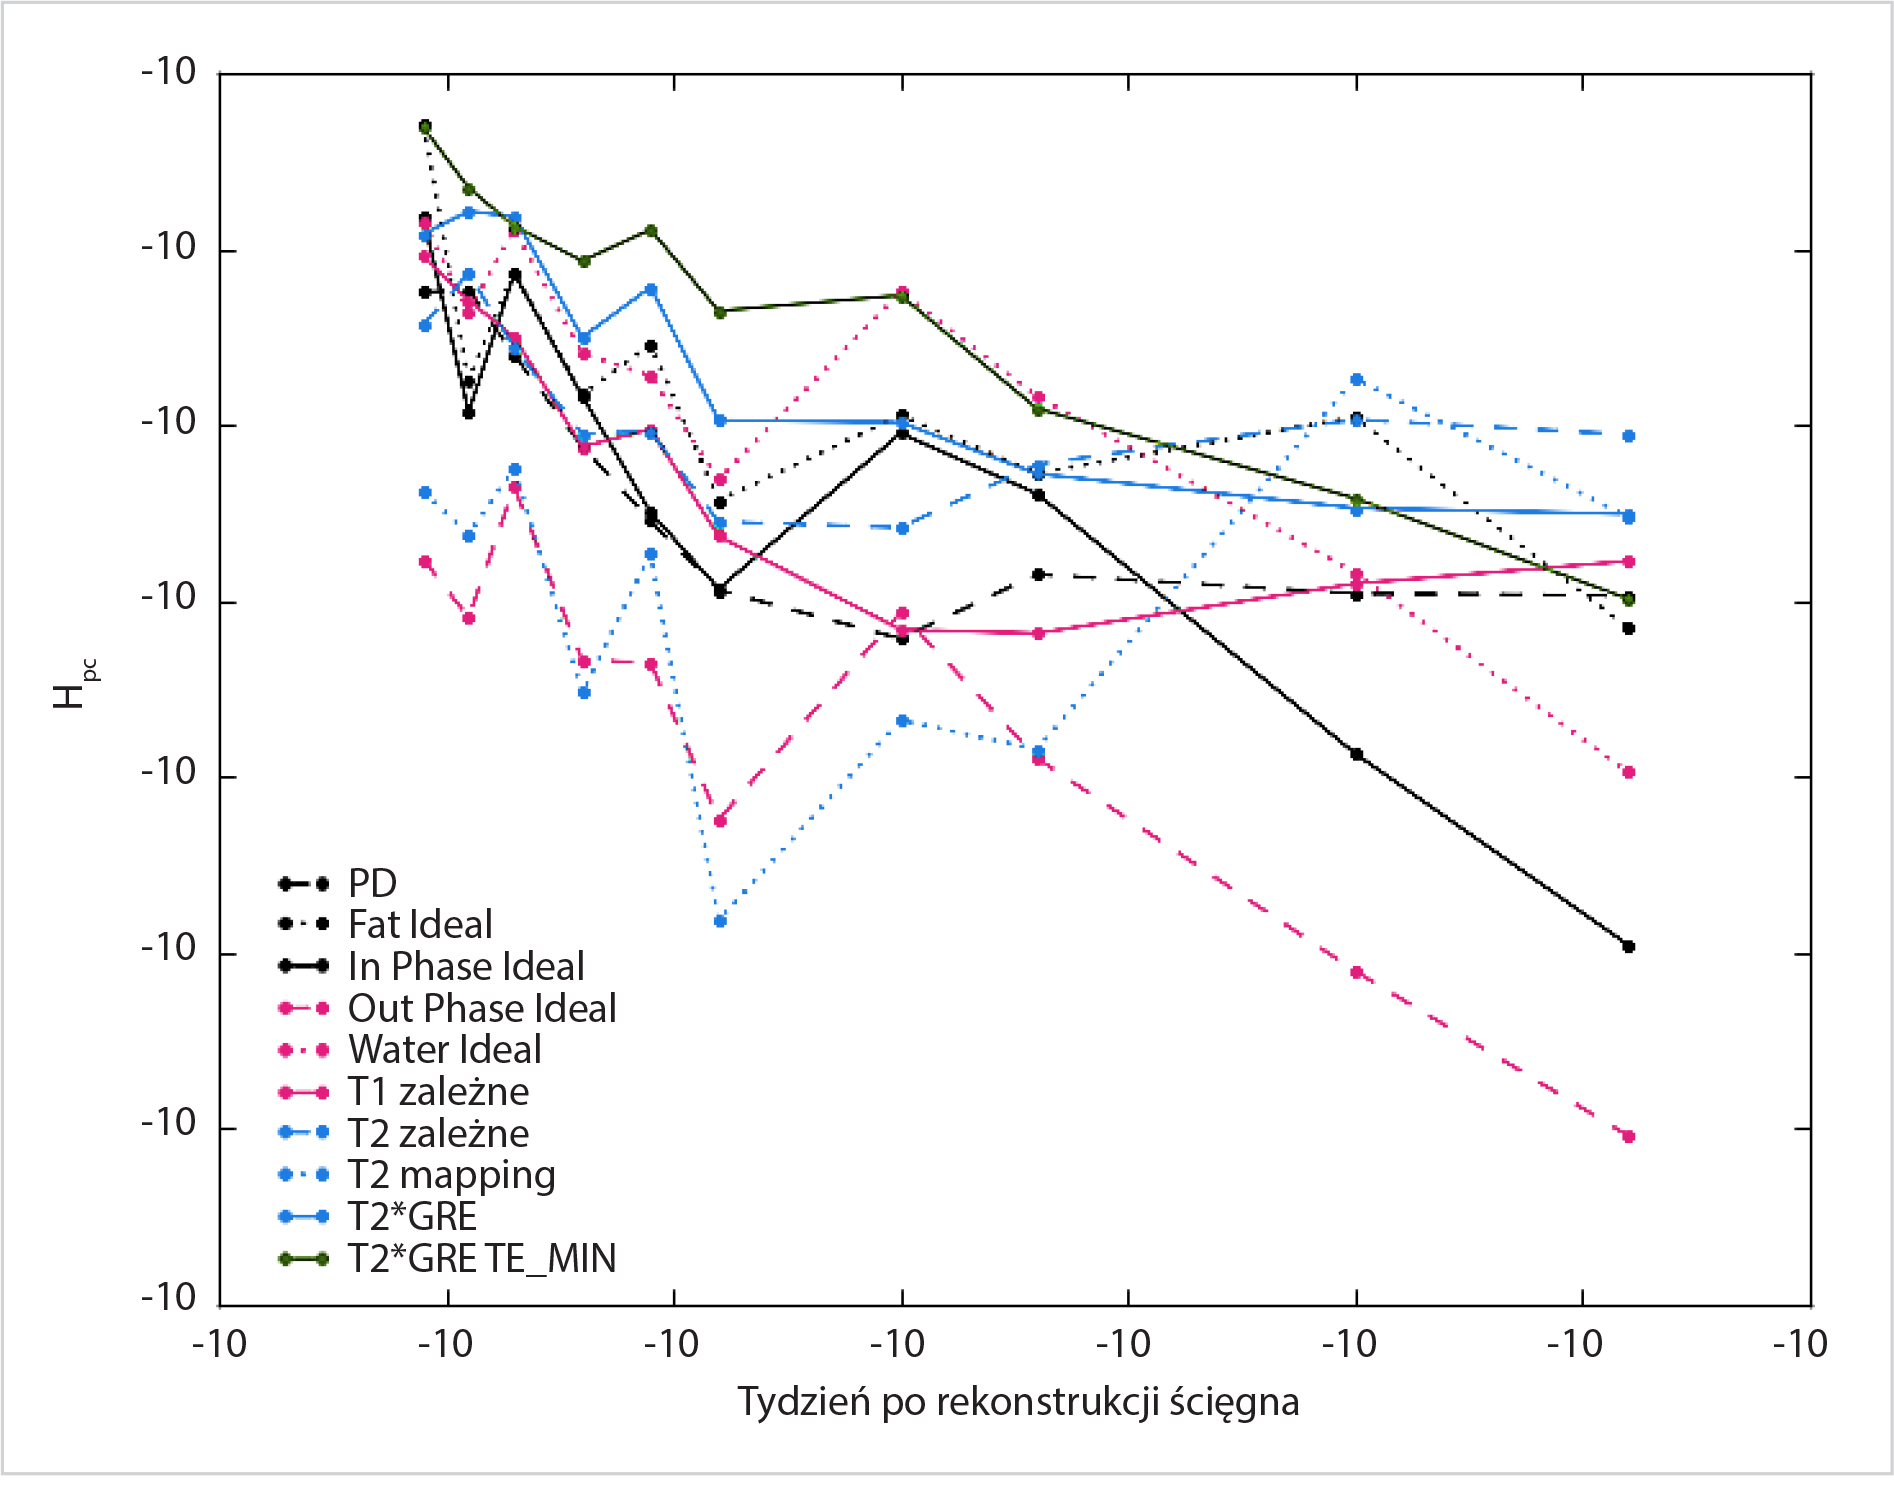
\includegraphics[width=1\textwidth]{figures/H_PC1.jpg}
	\caption{Porównanie krzywych dla 10 modalności RM reprezentujących średnią $H_{PC}$ z 10 pacjentów.}\label{fig:H}
\end{figure}
Oddzielnie przedstawiono wykresy uzyskanych krzywych dla wszystkich użytych w tej pracy sekwencji i modalności RM. W celu uzyskania pojedynczej wartości opisującej badanie RM wykorzystano ponownie średnią trymowaną:

\begin{equation}
\label{ecq:HPC}
H_{PC} = TM(PC1(x_1), PC1(x_2),..., PC1(x_n)).
\end{equation}

Wizualizacja umożliwia lepsze zrozumienie informacji zachowywanej przez użytą transformację PCA. Oprócz sekwencji T2 mapping, wszystkie pozostałe pokazują malejący trend rozumiany jako ujemna różnica pomiędzy wartością końcową i początkową okresu rehabilitacji. Odmienny trend T2 mapping może być spowodowany faktem, że dla tej sekwencji dane były zbierane we wszystkich 8-miu poziomach sygnału T2. W związku z tym, w obrazach pojawiają się próbki silnie zaszumione \linebreak i zniekształcone. Dopiero głębsza analiza związana np. z wyliczeniami na podstawie aproksymacji wartości poziomów T2 może skutkować efektywnym wykorzystaniem T2 mapping do oceny zadanego w tej pracy problemu (zob. \cite{Regulski2017}). 

W pozostałych przypadkach zaobserwować można istotne z punktu widzenia oceny gojenia etapy. Na początku procesu zmiany w badaniach obrazowych są bardzo wyraźne, co uwidocznione jest w postaci charakterystycznych minimów i maksimów lokalnych występujących do 20-tego tygodnia, gdzie wprowadzane są obciążanie nogi i kolejny etap rehabilitacji. Po tym okresie proces gojenia jest mniej dynamiczny. Ten ogólny schemat zaburzony jest przez fluktuacje zależne od indywidualnych cech pacjenta oraz czynników takich jak przestrzeganie zaleceń rehabilitacji, diety i aktywności pacjenta. 

Podsumowując, użyta transformacja pozwala na uzyskanie zredukowanego wektora cech DL, zawierającego od 1 do 200-stu wartości i zachowującego 50,2--98,8\% informacji. Średnie trendy tak otrzymywanych wartości wskazują również na możliwość wnioskowania co do procesu gojenia się ścięgna.  


\subsection{Wybór sekwencji rezonansu magnetycznego}
\label{seq:protocol_selection}
Z uwagi na opisany w p. \ref{RM} tor akwizycji danych RM, zwiększanie liczby sekwencji odbywa się kosztem wydłużenia czasu badania pacjenta. W skrajnym przypadku, takim jak pozyskanie wszystkich 10-ciu omawianych sekwencji, czas ten w nowoczesnych systemach wynosi około jednej godziny, co stanowi praktyczne ograniczenie opracowywanej metody. Dlatego celem tego eksperymentu jest wybór protokołu zawierającego minimalną liczbę sekwencji, umożliwiających przy użyciu opracowywanej metody skuteczną ocenę procesu gojenia. Prace podzielono na dwa etapy: analizę wizualną i ilościową.

\subsubsection{Analiza wizualna} W ramach wstępnej analizy, wartości danych ze wszystkich sekwencji i modalności zebranych od pacjentów zostały zakumulowane w postaci  histogramów i przedstawione na Rys. \ref{fig:Hists}.
\begin{figure}[]
	\centering
	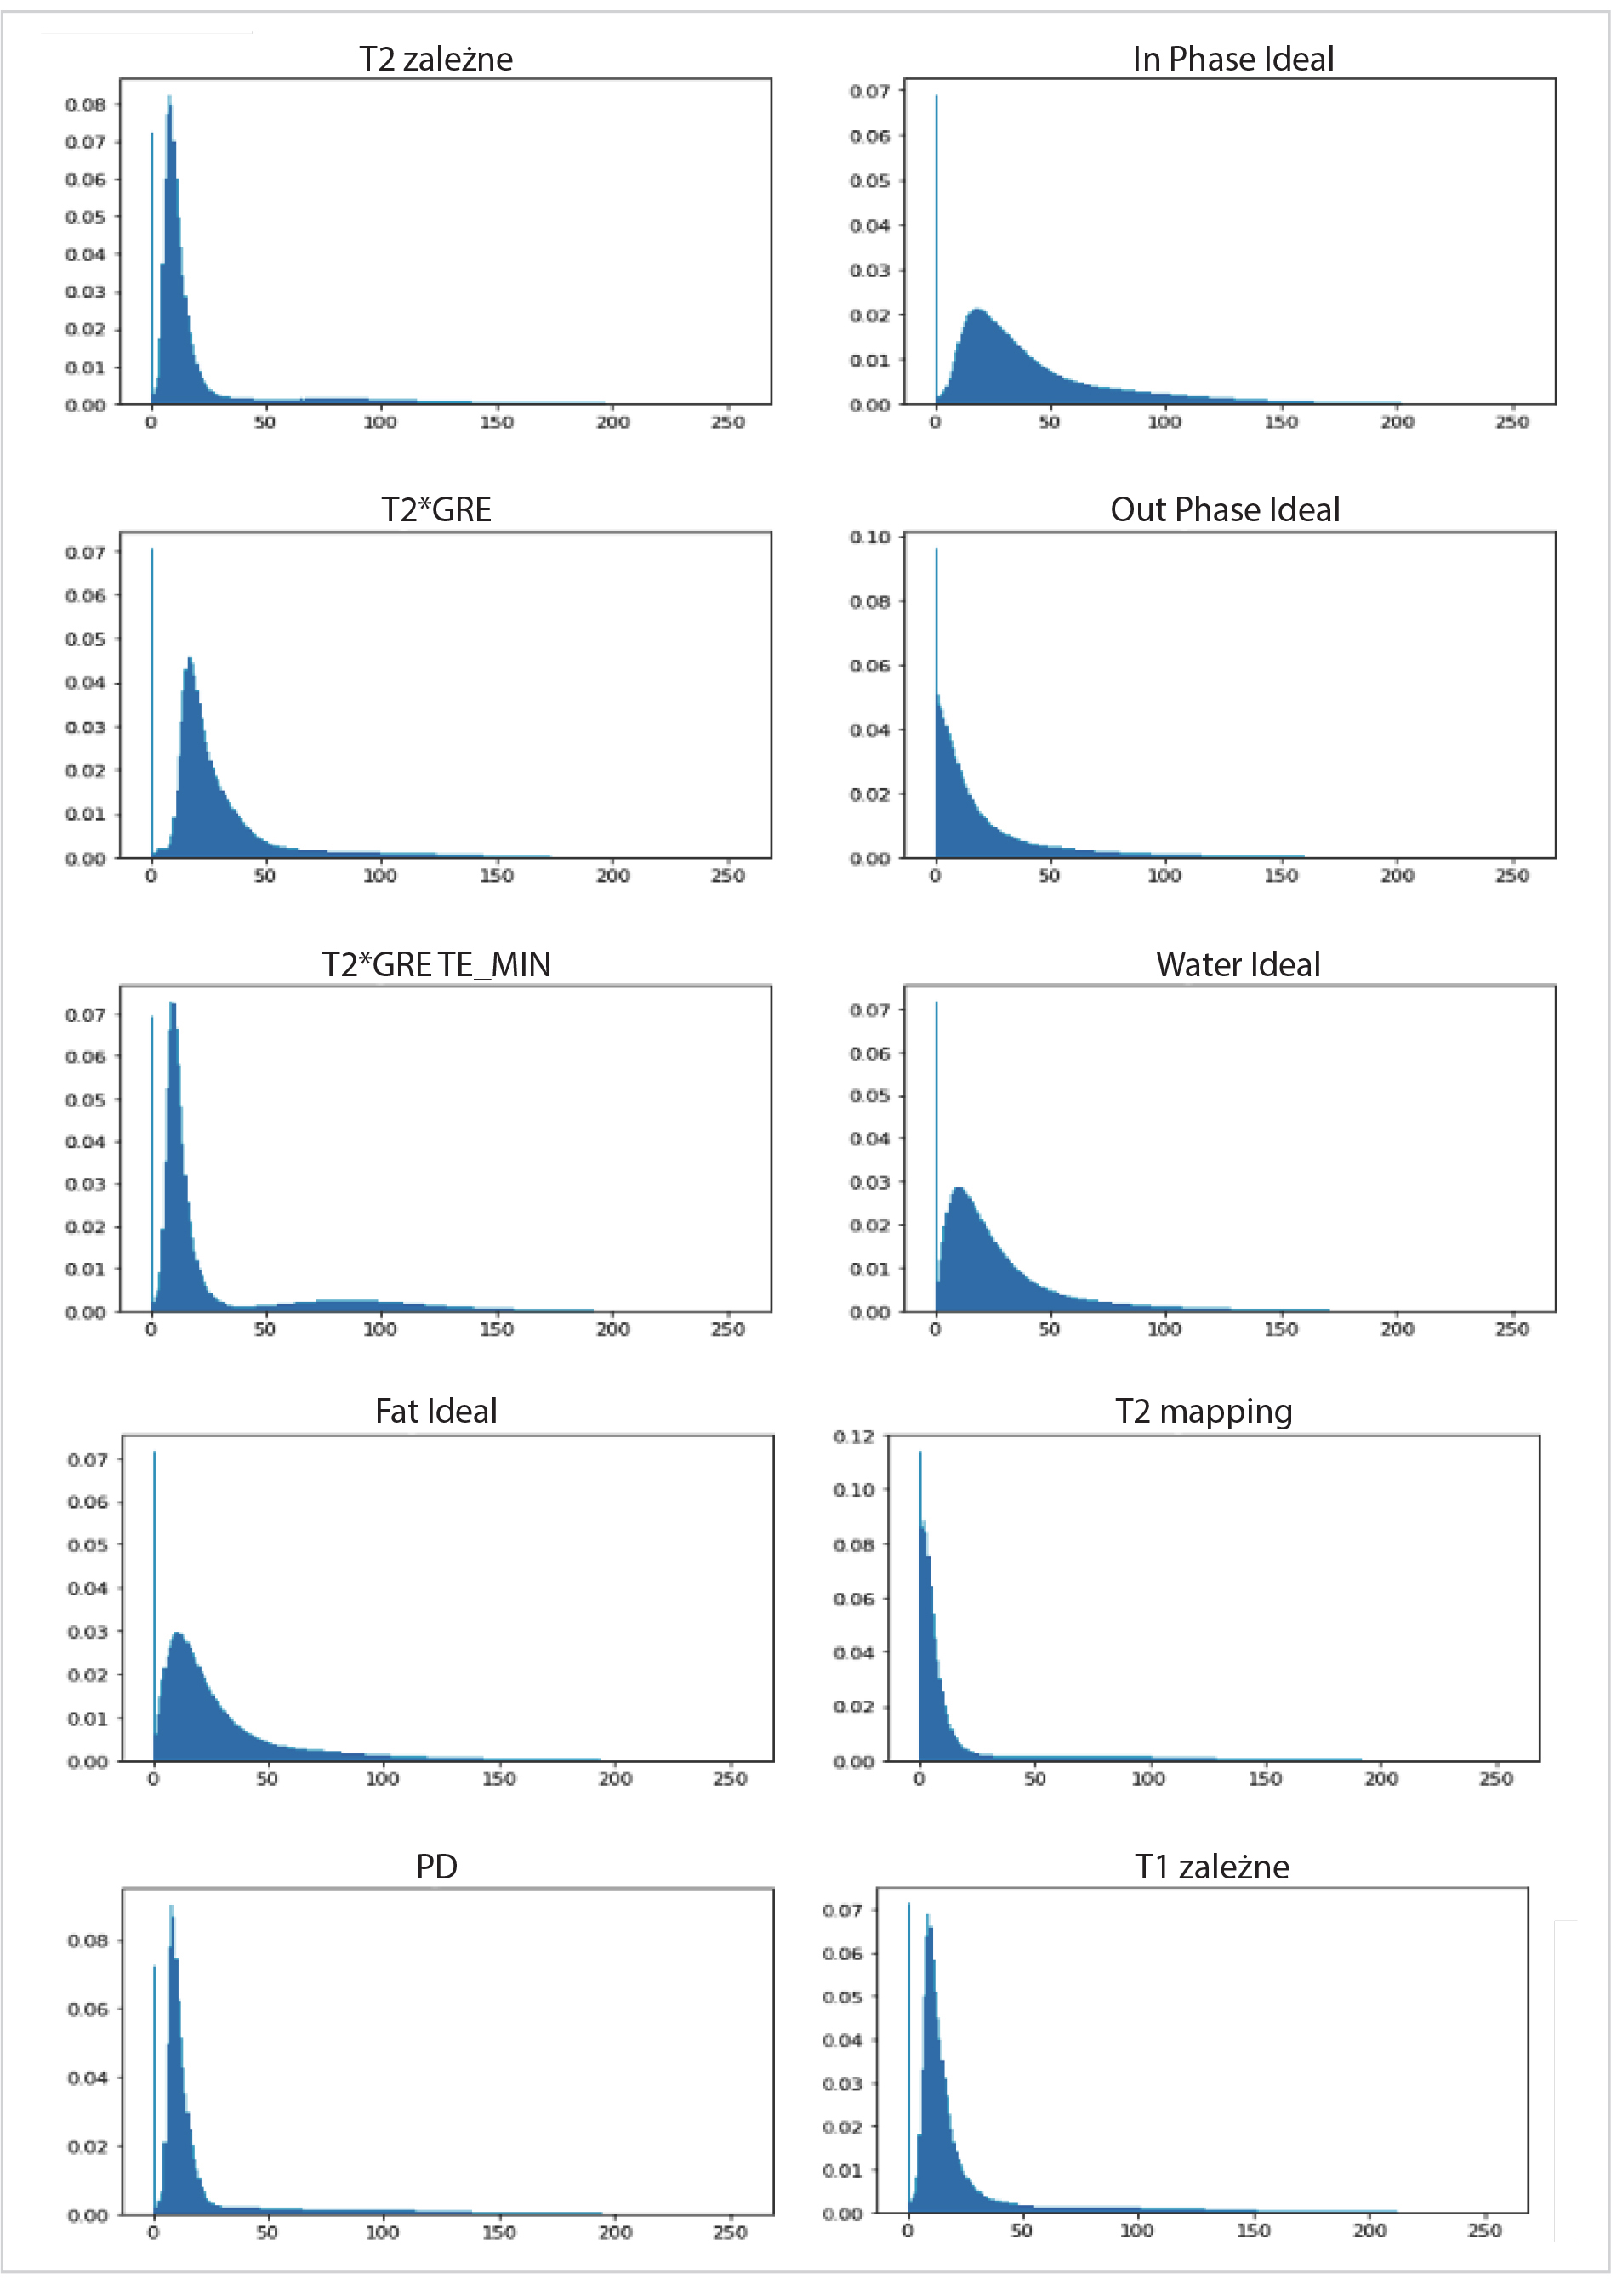
\includegraphics[width=1\textwidth]{figures/Hists.jpg}
	\caption{Znormalizowane histogramy dla 10-ciu sekwencji RM.}\label{fig:Hists}
\end{figure}
Dane zostały przeskalowane do zakresu $<$0; 255$>$ i zmodyfikowane do porównań tak, aby wartość całki Riemanna była równa 1.

Widoczne we wszystkich przypadkach maksima globalne w zerze są naturalnie wynikiem tła, które stanowi powietrze. Analizując pozostałe wartości można wyróżnić następujące 3 grupy:

\begin{enumerate}[noitemsep,nolistsep]
	\item Bez maksimum lokalnego -- sekwencja T2 mapping i modalność Out Phase Ideal. W pierwszym przypadku jest to konsekwencja, wspomnianego już w poprzednim eksperymencie, występowania danych ze wszystkich 8-miu próbek sekwencji, czyli również tych mierzonych przy prawie zerowym sygnale T2, silnie zaszumionym, z licznymi wartościami bliskimi zeru. W drugim przypadku, na granicach wody i tłuszczu, występuje często silne rozmycie (tzw. \textit{artefakt czarnego atramentu}), co również zwiększa liczbę wartości bliskich zeru.
	\item Z jednym maksimum lokalnym -- pozostałe modalności 3D FSPGR oraz sekwencje: PD, T1 zależne, T2 zależne, T2$^\ast$ GRE. Przypadek najczęściej występujący. Wartości sygnału zależą od tkanek dominujących w obrazowanym elemencie.
	\item Z dwoma maksimami lokalnymi -- sekwencja T2$^\ast$ GRE TE\_MIN. Jako jedyna posiada drugie maksimum lokalne, co może wskazywać na zwiększoną czułość na wzorce zawarte w danych.  
	
\end{enumerate}
%dlaczego wyrzucamy 3DFSPGR?
Na podstawie powyższej analizy, z uwagi na możliwość występowania wysokiego szumu w sygnale oraz artefaktów, można wyłączyć z dalszych badań pierwszą grupę sekwencji. 

Zdecydowanie wyróżniająca się sekwencją jest T2$^\ast$ GRE TE\_MIN. W celu lepszego zrozumienia istotności różnic występujących na Rys. \ref{fig:protocol_comp} zestawiono przykład rekonstrukcji danych z wykorzystaniem sekwencji z obu analizowanych dalej grup (wyłączono sekwencję 3DFSPGR, której modalności podzieliły się pomiędzy grupy 1 i 2 i która we wstępnych badaniach charakteryzowała się dużym zaszumieniem). 

 \begin{figure}[h]
 	\centering
 	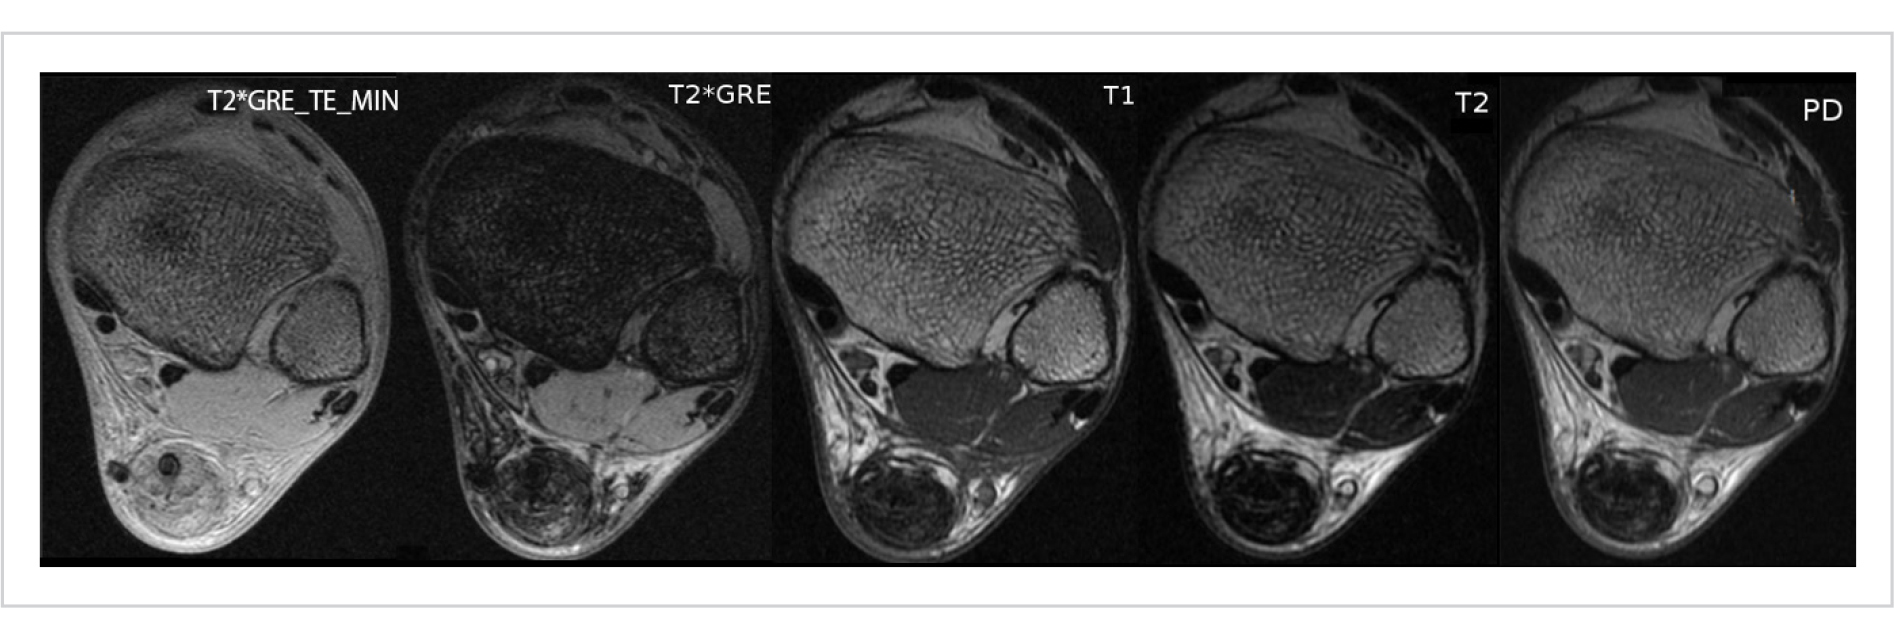
\includegraphics[width=1\textwidth]{figures/Protocol_comparison.jpg}
 	\caption{Porównanie sekwencji RM ilustrujących proces gojenia się ścięgna Achillesa w 12-tym tygodniu po rekonstrukcji.}\label{fig:protocol_comp}
 \end{figure}

Istotna różnica w rekonstruowanych obrazach pochodzi z poziomów odcieni szarości w obszarze ścięgna. Obrazy w dwunastym tygodniu procesu gojenia się, rekonstruowane przy pomocy sekwencji z grupy 2, charakteryzują się wartościami w obszarze ścięgna bliskimi zeru. Jedynie na obrazach rekonstruowanych z wykorzystaniem danych z T2$^\ast$ GRE TE\_MIN obszar ścięgna jest jaśniejszy. 

Na Rys. \ref{fig:T2comp} przedstawiono próbki T2$^\ast$ GRE TE\_MIN zrekonstruowane w kolejnych krokach czasowych.
\begin{figure}[h]
	\centering
	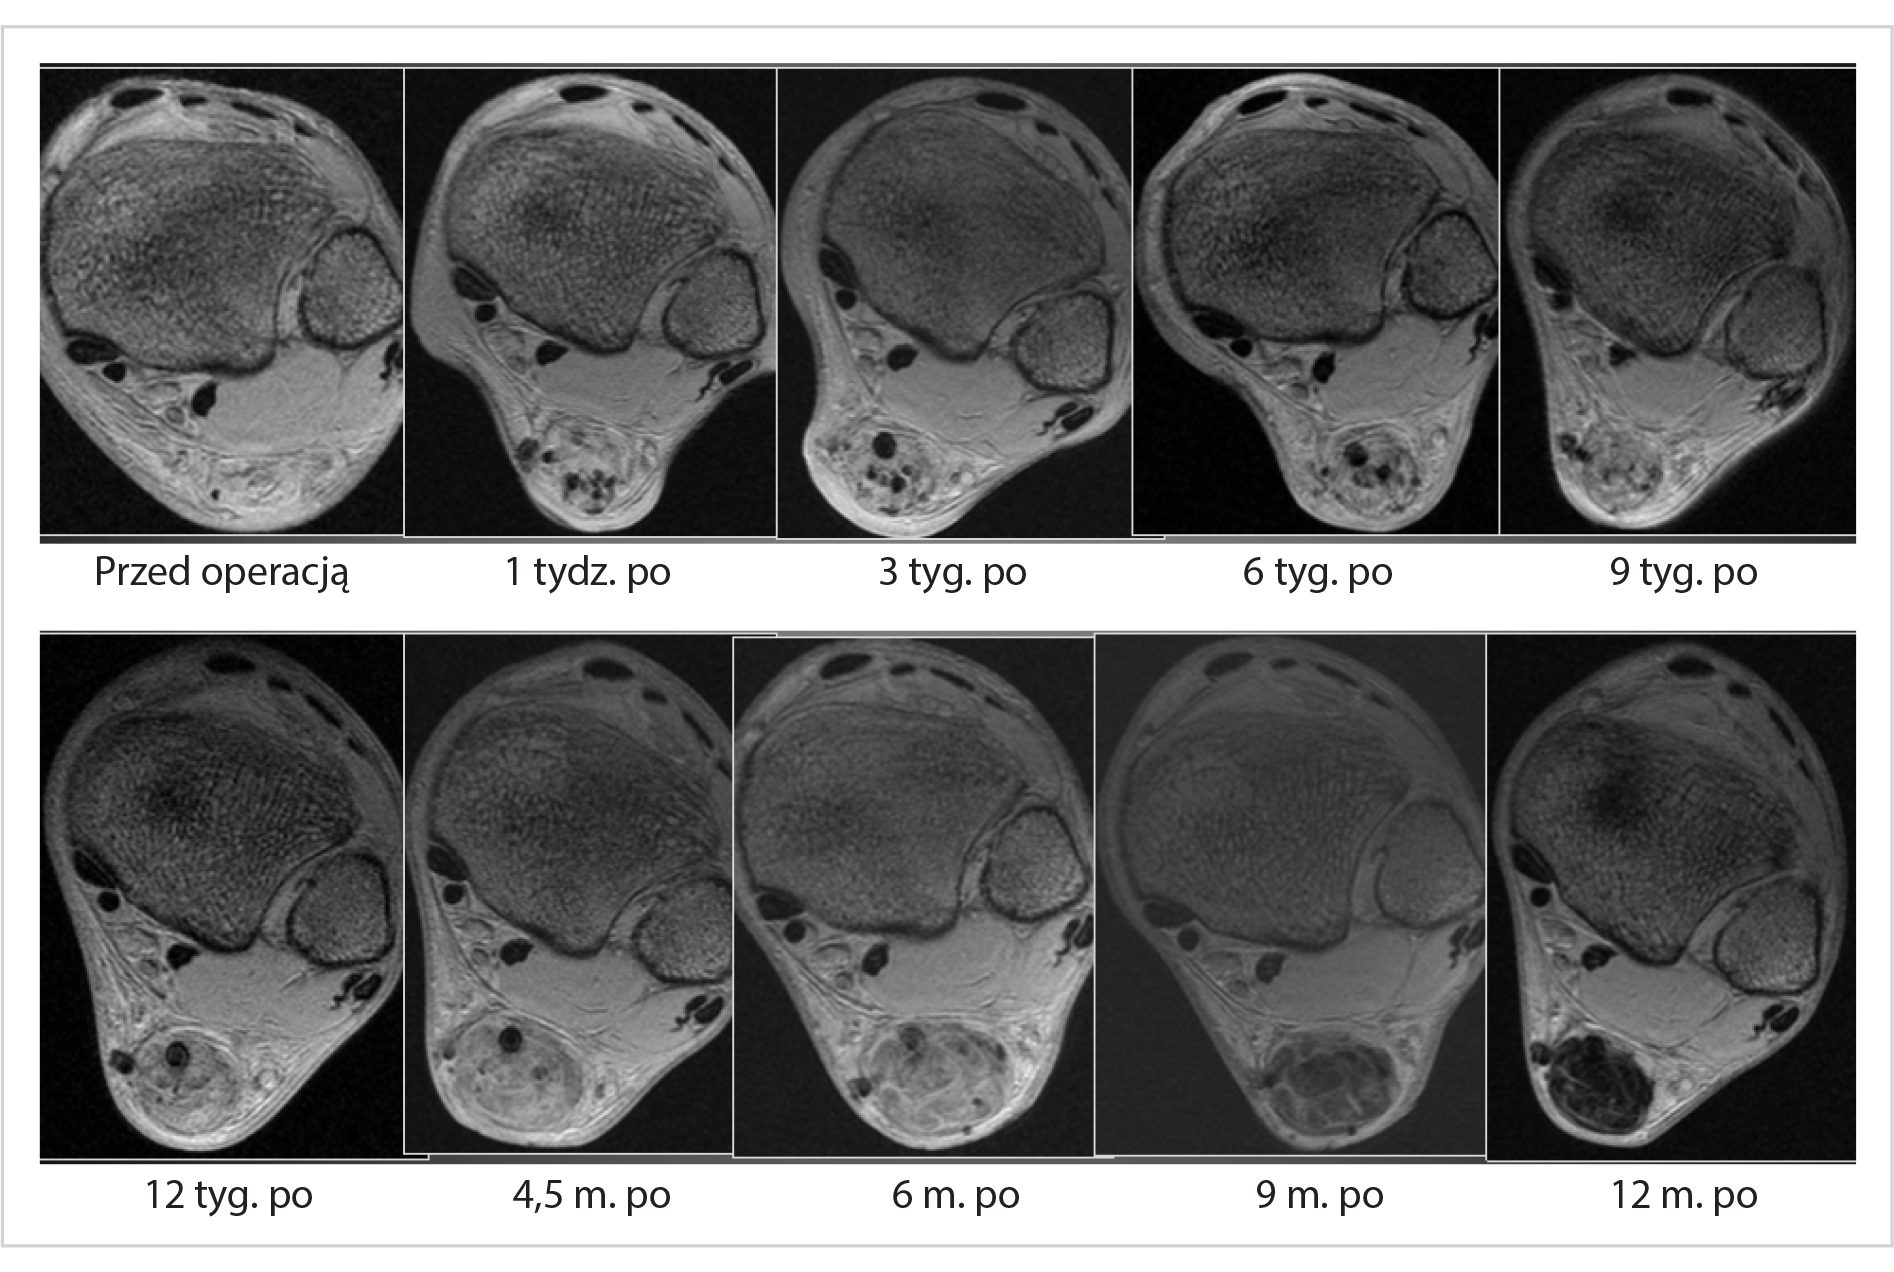
\includegraphics[width=1\textwidth]{figures/T2gremin.jpg}
	\caption{Proces gojenia się ścięgna Achillesa widoczny w obrazach zrekonstruowanych na podstawie danych z sekwencji T2$^\ast$ GRE TE\_MIN.}\label{fig:T2comp}
\end{figure}
Analiza wizualna wskazuje, że różnice w odcieniach szarości mogą wspomóc radiologów w skutecznej interpretacji stopnia wygojenia się tkanek ścięgnistych. Wartości w obszarze ścięgna są jasne na początku i ciemnieją z czasem. 

W sekwencji T2$^\ast$ GRE TE\_MIN, czas TE jest bardzo krótki. W pozostałych sekwencjach wykorzystanych w tej pracy TE $\gg$ T2$^\ast$. Z uwagi na cechy mierzonej tkanki, generowany sygnał ma tendencję do szybkiego zaniku. W T2$^\ast$ GRE TE\_MIN jest on zatem mierzony przed tym faktem, a nie przy wartościach bliskich zeru. \linebreak Na przestrzeni całego procesu gojenia się ścięgna, zmiany uwidaczniają się w postaci silnie rozróżnialnych odcieni szarości w obszarze ścięgna, co z kolei jest również wartościową informacją z uwagi na zastosowane w tej pracy metody sztucznej inteligencji i przetwarzania obrazów. Powyższe obserwacje i wnioski zostały dalej wykorzystane w analizie ilościowej.

\subsubsection{Analiza ilościowa} W ramach tego badania porównano ilościowo wyniki automatycznej oceny procesu gojenia się ścięgna Achillesa przy użyciu danych: (1) tylko z sekwencji \linebreak T2$^\ast$ GRE TE\_MIN; (2) danych z sekwencji T2$^\ast$ GRE TE\_MIN oraz PD i T2$^\ast$ GRE. 
Wybierając sekwencję T2$^\ast$ GRE TE\_MIN kierowano się wynikami analizy wizualnej, natomiast dobór pozostałych dwóch sekwencji, poza analizą wizualną i wiedzą dziedzinową, był umotywowany oceną stopnia korelacji zaprezentowaną w Tab. \ref{tab:inter-protocol-corr}, gdzie zestawiono sekwencje z grupy (2) bez 3DFSPGR.
\vspace{10px}
\renewcommand{\arraystretch}{1.2}
\begin{table}[h]
	\centering
	\setlength{\tabcolsep}{12pt}
	\caption{Korelacja sekwencji PD, T1, T2 i T2$^\ast$ GRE MRI. Wyniki oznaczone pogrubieniem są istotne statystycznie z $p$ $<$ 0,01.}
	\label{tab:inter-protocol-corr}
	\begin{tabular}{l||c|c|c|c}
		%\hline
		& PD & T1 & T2 & T2$^\ast$GRE \\ \hline \hline
		PD & 1,00 & \textbf{0,96} & \textbf{0,90} & \textbf{0,89} \\ \hline
		T1 & \textbf{0,96} & 1,00 & \textbf{0,85} & \textbf{0,92} \\ \hline
		T2 & \textbf{0,90} & \textbf{0,85} & 1,00 & 0,71 \\ \hline
		T2$^\ast$GRE & \textbf{0,89} & \textbf{0,92} & 0,71 & 1,00  %\hline
	\end{tabular}
	%\vspace{-0.5cm}
\end{table} 
\renewcommand{\arraystretch}{1}

Do obliczeń korelacji wybrano wektor cech DL zredukowany do pojedynczej wartości niosącej ponad 50\% informacji, zagregowany dla badania z wykorzystaniem metryki $H_{PC}$ (zob. wzór \ref{ecq:HPC}). Uwzględniając wyniki istotne statystycznie, wśród najbardziej skorelowanych sekwencji znalazły się T1 i PD. PD najmniej koreluje \linebreak z T2$^\ast$GRE, natomiast T1 z sekwencją T2. 

W kolejnym kroku wykorzystano tę informację sprawdzając, w odniesieniu \linebreak do wybranej w analizie wizualnej sekwencji T2$^\ast$ GRE TE\_MIN, czy wnioskowanie co do procesu gojenia, na podstawie cech DL ulega polepszeniu z wykorzystaniem większej liczby różnorodnych sekwencji. 

Wykorzystano ponownie zredukowaną przestrzeń cech DL (tym razem 1--10 czynników głównych) i wykonano szereg obliczeń stopnia gojenia się ścięgna stosując poniższą metrykę: 

\begin{equation}
H_{reg} = \alpha + \sum_{i=1}^{3}\beta_{i}X_{i} + \sum_{i=1}^{3}\gamma_{i}X_{i}^{2} +
\sum_{\substack{i, j = 1\\ i < j}}^{3}\lambda_{i,j}X_{i}X_{j}
\end{equation}

gdzie $X_i = TM(PC_n(x_1), PC_n(x_2),..., PC_n(x_n))_{i}$ to kolejne predyktory odpowiadające próbkom z trzech wykorzystywanych w eksperymencie sekwencji, $TM$ \linebreak to średnia trymowana z marginesami 2,5\%, $PC_n(x_k)$ to $n$-ty czynnik główny otrzymany przy wnioskowaniu sieci dla przekroju osiowego $x_k$, a $k$ jest indeksem przekroju danej sekwencji w trójwymiarowym badaniu RM.

W szczególności, wyliczono różne modele regresji poczynając odpowiednio od liniowej, gdzie ($\gamma_{i}=0, \lambda_{i}=0$), przez nieliniową stopnia drugiego -- $model\_poly$ ($\lambda_{i}=0$) oraz z kombinacją czynników -- $model\_c\_poly$. W przypadku liniowym wykorzystano 1--10 czynników głównych -- odpowiednio $model\_PC[1-10]$. Natomiast w przypadku nieliniowym wykorzystano tylko dwa pierwsze czynniki, ograniczając tym samym efekt nadmiernego dopasowania się modelu. Powyższe modele funkcjonujące w oparciu o trzy sekwencje (tj. T2$^\ast$ GRE TE\_MIN, PD i T2$^\ast$ GRE) zestawiono z modelem liniowej regresji wytrenowanym jedynie na danych z T2$^\ast$ GRE TE\_MIN ($Baseline$). 

Do obliczenia współczynników regresji zastosowano zbiór pacjentów treningowych. Natomiast w celach porównań, zestawiono wyniki dla pacjentów testowych. \linebreak W szczególności, wyliczono metryki średniego błędu absolutnego (MAE), maksymalnego błędu absolutnego (MAX-AE) i średniej korelacji obliczonej z wykorzystaniem transformacji Z-Fishera (Corr). Wybór metryk związanych z błędami absolutnymi był podyktowany faktem, iż skala liniowa okazała się w toku eksperymentów bardziej intuicyjna dla lekarzy i radiologów, a zatem bardziej utylitarna w procesie komunikowania wyników. Rezultaty znajdują się w Tab. \ref{tab:H_testset}.
\renewcommand{\arraystretch}{1.2}
\begin{table}[h!]
	\caption{Porównanie wnioskowania dla różnych modeli regresji wytrenowanych w oparciu o dane z 3-ech sekwencji RM, z modelem liniowej regresji wytrenowanym w oparciu o jedną sekwencję RM. Najlepsze wyniki oznaczono pogrubieniem i dodatkowo, w przypadku istotnej statystycznie poprawy z $p$ $<$ 0,05 liczonych średnich, oznaczono kolorem czerwonym.}
	\scriptsize
	\begin{center}
		\begin{tabular}{lc||c|c|c|c|c|c}
			\textbf{Model} & & \textbf{SCT} & \textbf{TT} & \textbf{STE} & \textbf{TE} & \textbf{TU} & \textbf{TisE}\\ 
			
			\hline \hline
			model\_PC1 & MAE & 1,26 $\pm$ 0,07 & \textcolor{red}{\textbf{0,71}} $\pm$ 0,02 & \textbf{0,7} $\pm$ 0,02 & 0,97 $\pm$ 0,04 & 0,92 $\pm$ 0,04 & 0,99 $\pm$ 0,04\\
			&MAX-AE &3,53&2,49&1,91&\textbf{2,34}&2,2&2,47\\
			&Corr &0,58&0,47&-0,07&0,60&\textbf{0,56}&0,58\\
			
			\hline
			model\_PC1\_2 & MAE & 1,28 $\pm$ 0,07 & 0,74 $\pm$ 0,02 & 0,71 $\pm$ 0,03 & 0,98 $\pm$ 0,04 & 0,94 $\pm$ 0,05 & 1,02$\pm$ 0,04\\
			&MAX-AE &3,64&2,56&1,94&2,98&2,35&2,9\\
			&Corr &0,53&0,30&0,02&0,51&0,41&0,60\\
			
			\hline
			model\_PC1\_3&MAE & 1,43 $\pm$ 0,09 & 0,71 $\pm$ 0,02 & 0,73 $\pm$ 0,03 & 1,02 $\pm$ 0,05 & 1,05 $\pm$ 0,05 & 1,07 $\pm$ 0,06\\
			&MAX-AE &3,99&2,49&1,98&3,2&2,96&3,02\\
			&Corr &0,48&0,36&0,03&0,50&0,29&0,62\\
			
			\hline
			model\_PC1\_4&MAE & 1,39 $\pm$ 0,08 & 0,72 $\pm$ 0,01 & 0,8 $\pm$ 0,02 & 1,01 $\pm$ 0,04 & 1,02 $\pm$ 0,05 & 1,06 $\pm$ 0,05\\
			&MAX-AE &3,56&\textbf{2,4}&2,17&3,2&2,61&3,13\\
			&Corr &0,54&0,37&0,17&0,52&0,38&\textbf{0,68}\\
			
			\hline
			model\_PC1\_5&MAE & 1,35$\pm$ 0,07 & 0,79$\pm$0,01 &0,8$\pm$0,04 &0,99$\pm$0,04 &1,01$\pm$0,04 &1,1$\pm$0,04\\
			&MAX-AE &3,45&2,69&2,39&3,21&2,55&2,88\\
			&Corr &0,49&0,31&0,22&0,52&0,30&0,60\\
			
			\hline
			model\_PC1\_6&MAE & 1,32$\pm$0,07 & 0,78$\pm$0,01 &0,8$\pm$0,04& 0,97$\pm$0,05 & 0,98$\pm$0,04 &1,11$\pm$0,04\\
			&MAX-AE &\textbf{3,3}&2,64&2,21&3,12&2,6&2,8\\
			&Corr &0,53&0,33&0,21&0,56&0,38&0,56\\
			
			\hline
			model\_PC1\_7&MAE &$1,33\pm{0,07}$&$0,78\pm{0,01}$&$0,82\pm{0,04}$&$1,03\pm{0,05}$&$0,99\pm{0,04}$&$1,14\pm{0,05}$\\
			&MAX-AE &3,34&2,75&2,41&3,17&2,63&2,69\\
			&Corr &0,53&0,33&0,21&0,54&0,30&0,57\\
			
			\hline
			model\_PC1\_8&MAE & 1,35$\pm$0,07 & 0,77$\pm$0,01& 0,81$\pm$0,04&1,02$\pm$0,05& 0,99$\pm$0,05 & 1,14$\pm$0,05\\
			&MAX-AE &3,41&2,58&2,47&3,13&2,65&2,75\\
			&Corr &0,54&0,37&0,19&0,53&0,25&0,55\\
			
			\hline
			model\_PC1\_9&MAE & 1,38$\pm$0,07 & 0,74$\pm$0,01 & 0,76$\pm$0,05 & 1,03$\pm$0,05 & 1,02$\pm$0,05 & 1,12$\pm$0,04\\
			&MAX-AE &3,49&2,57&2,45&2,9&2,7&2,67\\
			&Corr &0,52&0,40&\textbf{0,25}&0,55&0,30&0,58\\
			
			\hline
			model\_PC1\_10&MAE & 1,37$\pm$0,07 & 0,74$\pm$0,02 & 0,76$\pm$0,04 & 1,04$\pm$0,04 & 1,03$\pm$ 0,05& 1,11$\pm$0,05\\
			&MAX-AE &3,46&2,42&2,52&2,92&2,67&2,68\\
			&Corr &0,50&0,38&0,24&0,54&0,29&0,59\\
			
			\hline
			model\_poly&MAE & 1,27$\pm$ 0,07 & 0,74$\pm$0,01 & 0,71$\pm$0,03 & \textcolor{red}{\textbf{0,93}}$\pm$0,04 & 0,95$\pm$0,05 & 1,03$\pm$0,04\\
			&MAX-AE &3,62&2,6&1,96&2,83&2,29&2,87\\
			&Corr &0,53&0,34&0,11&\textbf{0,61}&0,37&0,58\\
			
			\hline
			model\_c\_poly&MAE & 1,3$\pm$0,07 & 0,75$\pm$0,01 & 0,78$\pm$0,04 & \textcolor{red}{\textbf{0,93}}$\pm$0,04 & 1,01$\pm$0,06 & 1,06$\pm$0,05 \\
			&MAX-AE &3,64&2,7&2,01&2,83&3,36&2,86\\
			&Corr &0,53&0,45&0,12&0,58&0,15&0,57\\
			\hline 
			
			Baseline& MAE & \textbf{1,24}$\pm$0,08 & 0,82$\pm$0,04 & 0,75$\pm$0,04 & 1,06$\pm$0,05 & \textbf{0,90}$\pm$0,04 & \textbf{0,96}$\pm$0,05 \\
			&MAX-AE & 3,54 & 2,46 & \textbf{1,82} & 2,70 & \textbf{2,13} & \textbf{2,18}\\
			&Corr   & \textbf{0,61} & \textcolor{red}{\textbf{0,64}} &-0,08 & 0,55 & 0,55 & 0,65\\
			\hline
		\end{tabular}
	\end{center}
	\label{tab:H_testset}
\end{table}
\renewcommand{\arraystretch}{1}

Z wykorzystaniem dodatkowych sekwencji udało się uzyskać poprawę istotną statystycznie z $p$ $<$ 0,05 w przypadku MAE dla parametrów TT i TE. W przypadku TT dodanie sekwencji skutkowało natomiast istotnie statystycznym pogorszeniem Corr. Model prostej liniowej regresji wykorzystujący jedynie informacje z sekwencji T2$^\ast$ GRE TE\_MIN ponadto osiągnął najlepsze rezultaty w największej liczbie błędów MAX-AE tj. 3. Można zatem wnioskować, że dodawanie sekwencji jako danych wejściowych i komplikacje modelu skutkują nadmiernym dopasowaniem oraz po za opisanymi wyjątkami nie polepszają jakości automatycznej oceny. Należy również podkreślić, że akwizycja samej sekwencji T2$^\ast$ GRE TE\_MIN dla omawianego problemu zajmuje przy obecnym stanie techniki około 5 min. na pacjenta, podczas gdy wszystkich trzech sekwencji trwa około 12 minut. Podsumowując, na podstawie analizy wizualnej i ilościowej, jako dane wejściowe do kolejnych eksperymentów została wybrana sekwencja T2$^\ast$ GRE TE\_MIN. 

\subsection{Optymalna selekcja i konkatenacja cech}
\label{seq:fusion}
W poprzednim eksperymencie uzyskano najlepsze wyniki z wykorzystaniem modeli regresji liniowej. Można zatem postawić hipotezę, że w ocenie radiologa dominuje zależność liniowa. Dodatkowo, cechy obrazowe opisujące jeden problem diagnostyczny są ze sobą zazwyczaj silnie skorelowane. Stąd motywacja, aby w ramach tego eksperymentu do selekcji cech zastosować metodę LASSO (zob. pkt \ref{DimReduction}), bazującą właśnie na liniowych własnościach i znajdującą swe zastosowanie przy silnie skorelowanych predyktorach.  

W tym celu, treningowy zbiór pacjentów został podzielony na 4 podzbiory (11-tu pacjentów, około 4300 przekrojów osiowych) i wykorzystany do kroswalidacji. Wynikiem tych działań był dobór możliwie najlepszego parametru $\alpha$ dla metody LASSO (zob. wzór \ref{equ:lassoReg}). Jako dane wejściowe wykorzystano zbiór ograniczony do sekwencji T2$^\ast$ GRE TE\_MIN, z których dla każdego przekroju wyliczono odpowiednio 200 cech DL i 46 klasycznych cech obrazowych (zob. p. \ref{seq:method}).

Wyniki metody LASSO (tj. błąd średniokwadratowy powiększony o funkcję kary) dla każdego pacjenta zestawiono w krzywe łączące kolejne punkty obrazowania.
Kryterium selekcji cech była najlepsza korelacja wzorca odniesienia z krzywymi, którą uzyskano dla $\alpha=0,1$. W rezultacie, dla 6-ciu parametrów wzorca odniesienia uzyskano następujące podzbiory predyktorów:  
\begin{itemize}[noitemsep,nolistsep]
	\item SCT: 6 cech DL (PC1, PC2, PC3, PC5, PC7, PC9), 10 klasycznych cech obrazowych, w tym 3 cechy Haralicka (suma wariancji dla dystansu separacji $d$ = 1, suma średnich dla $d$ = 5 i suma średnich dla $d$ = 10);
	\item TT: 5 cech DL (PC1, PC2, PC3, PC4, PC5) i 7 klasycznych cech obrazowych bez udziału cech Haralicka;
	\item STE: 5 cech DL (PC1, PC4, PC7, PC8, PC9) i 8 klasycznych cech obrazowych bez udziału cech Haralicka;
	\item TE: 4 cechy DL (PC1, PC2, PC3, PC9) i 8 klasycznych cech obrazowych, \linebreak w tym jedna cecha Haralicka tj. suma średnich dla $d$ = 10;
	\item TU: 4 cechy DL (PC1, PC3, PC4, PC9) i 9 klasycznych cech obrazowych, \linebreak w tym jedna cecha Haralicka tj. suma wariancji dla $d$ = 1;  
	\item TisE: 6 cech DL (PC1, PC2, PC3, PC5, PC7, PC9) i 7 klasycznych cech obrazowych bez udziału cech Haralicka.
	
\end{itemize}
Maksymalna liczba cech w zredukowanej przestrzeni wyniosła 16 dla parametru SCT. Ponadto cechy DL i klasyczne cechy obrazowe są obecne w każdym z ocenianych kryteriów wzorca odniesienia, co wskazuje na możliwość uzyskania polepszonych rezultatów oceny z wykorzystaniem fuzji. Należy również zwrócić uwagę, \linebreak że największa liczba cech Haralicka (tj. 3) występuje w parametrze SCT związanym z oceną struktury włókien widoczną w obrazach jako różne tekstury.

Wyselekcjonowane podzbiory wykorzystano w kolejnym kroku eksperymentu, mając na celu porównanie oceny procesu gojenia przy zastosowaniu różnych metod. Wykorzystano zarówno liniową regresję jak i algorytmy mogące modelować nieliniowe zależności. Pomimo wstępnego założenia o dominacji liniowych związków np. wynik modelu $model\_poly$ dla Corr w parametrze TE (zob. Tab. \ref{tab:H_testset}) pozwala zakładać, że ocena w niektórych detalach może mieć również charakter nieliniowy. 

Dlatego w porównaniu metod meta-regresji cech uwzględniono: metodę wektorów nośnych (SVR -- od ang. \textit{Support Vector Regression}) opisaną w \cite{SVR_drucker}, wielowarstwowy perceptron liniowy z 4-ema neuronami w warstwie ukrytej (MPR -- od ang. \textit{Multilayer Perceptron Regression}) oraz las losowy składający się ze 100 drzew decyzyjnych (RF -- od ang. Random Forest). Wyniki zestawiono w Tab. \ref{tab:trainset} z rezultatami liniowej regresji (LR -- od ang. Linear regression) i regresji nieliniowej drugiego stopnia (Poly -- od ang. Polynomial). Trening metod i dobór hiperparametrów wykonano z wykorzystaniem kroswalidacji z podziałem na 4 segmenty i zbioru treningowego pacjentów.

\begin{table*}[]
	\caption{Wyniki oceny procesu gojenia z wykorzystaniem fuzji cech i zbioru treningowego.}
	\scriptsize
	\begin{center}
		\begin{tabular}{lc||c|c|c|c|c|c}
			\textbf{Model} & & \textbf{SCT} & \textbf{TT} & \textbf{STE} & \textbf{TE} & \textbf{TU} & \textbf{TisE}\\ 
			
			\hline \hline
			\multirow{3}{*}{Poly}
			& MAE & $1,00\pm0,03$ & $0,62\pm0,02$ & $0,73\pm0,02$ & $0,76\pm0,02$ & $0,89\pm0,03$ & $0,70\pm0,02$\\
			& MAX-AE & 3,53 & 2,35 & 3,62 & 2,49 & 2,90 & 2,64 \\
			& Corr   & 0,87 & 0,82 & 0,46 & 0,80 & 0,65 & 0,87 \\
			\hline
			\multirow{3}{*}{SVR}
			& MAE & $0,88\pm0,01$ & $0,59\pm0,01$ & $0,67\pm0,01$ & $0,69\pm0,01$ & $0,83\pm0,01$ & $0,63\pm0,01$\\
			& MAX-AE & 3,73 & 2,32 & 3,83 & 2,50 & 2,95 & 2,75 \\
			& Corr   & 0,89 & 0,85 & 0,59 & 0,83 & 0,72 & 0,88 \\
			\hline
			\multirow{3}{*}{LR}
			& MAE & $1,00\pm0,04$ & $0,62\pm0,02$ & $0,74\pm0,02$ & $0,74\pm0,02$ & $0,90\pm0,03$ & $0,69\pm0,02$\\
			& MAX-AE & 3,52 & 2,39 & 3,77 & 2,52 & 2,88 & 2,65 \\
			& Corr   & 0,87 & 0,83 & 0,46 & 0,80 & 0,65 & 0,87 \\
			\hline
			\multirow{3}{*}{MPR}
			& MAE & $1,00\pm0,04$ & $0,63\pm0,02$ & $0,74\pm0,02$ & $0,71\pm0,02$ & $0,88\pm0,03$ & $0,96\pm0,02$\\
			& MAX-AE & 3,47 & 2,51 & 3,57 & 2,52 & 2,86 & 2,65 \\
			& Corr   & 0,86 & 0,83 & 0,46 & 0,80 & 0,65 & 0,88 \\
			\hline
			 \multirow{3}{*}{RF}
			 & MAE & $0,32\pm0,04$ & $0,21\pm0,02$ & $0,25\pm0,03$ & $0,25\pm0,02$ & $0,31\pm0,03$ & $0,23\pm0,02$\\
			 & MAX-AE & 1,24 & 0,82 & 1,33 & 0,89 & 1,03 & 0,92 \\
			 & Corr   & 0,99 & 0,99 & 0,99 & 0,99 & 0,99 & 0,99 \\
			 \hline
		\end{tabular}
	\end{center}
	\label{tab:trainset}
\end{table*}

Do oceny ponownie wykorzystano metryki średniego błędu absolutnego (MAE), maksymalnego błędu absolutnego (MAX-AE) i średniej korelacji obliczonej z wykorzystaniem transformacji Z-Fishera (Corr). Najlepszy rezultat dla każdego z parametrów uzyskano dla lasu losowego, jednak w przypadku tego algorytmu (pomimo wielu prób z różną liczbą drzew decyzyjnych) występuje efekt nadmiernego dopasowania, co można zaobserwować analizując wyniki ze zbioru testowego zestawione \linebreak w Tab. \ref{tab:testset}. 

\begin{table*}[]
	\caption{Wyniki oceny procesu gojenia z wykorzystaniem fuzji cech i zbioru testowego. Pogrubieniem oznaczono najlepsze wyniki uzyskane przez algorytmy meta-regresji z wyłączeniem RF, dla którego występuje efekt przeuczenia. Dodatkowo, w przypadku istotnej statystycznie poprawy z $p$ $<$ 0,05 liczonych średnich, wyniki najlepsze oznaczono kolorem czerwonym.}
	\scriptsize
	\begin{center}
		\begin{tabular}{lc||c|c|c|c|c|c}
			\textbf{Model} & & \textbf{SCT} & \textbf{TT} & \textbf{STE} & \textbf{TE} & \textbf{TU} & \textbf{TisE}\\ 
			
			\hline \hline
			\multirow{3}{*}{Poly}
			& MAE & $1,15\pm0,06$ & $0,57\pm0,03$ & $0,75\pm0,04$ & $0,94\pm0,05$ & $0,92\pm0,04$ & \textbf{0,94}$\pm0,05$\\
			& MAX-AE & 2,67 & 1,78 & 1,81 & \textbf{2,50} & 2,12 & 2,39 \\
			& Corr   & 0,82 & 0,83 & 0,25 & 0,71 & 0,63 & 0,78 \\
			\hline
			\multirow{3}{*}{SVR}
			& MAE & \textcolor{red}{\textbf{1,05}}$\pm0,06$ & $0,56\pm0,03$ & $0,75\pm0,04$ & $0,91\pm0,05$ & $0,91\pm0,04$ & \textbf{0,94}$\pm0,05$\\
			& MAX-AE & 2,62 & 1,82 & 1,92 & 2,54 & \textbf{2,01} & 2,38 \\
			& Corr   & \textcolor{red}{\textbf{0,85}} & \textcolor{red}{\textbf{0,85}} & \textcolor{red}{\textbf{0,31}} & 0,72 & \textbf{0,65} & \textbf{0,80} \\
			\hline
			\multirow{3}{*}{LR}
			& MAE & $1,15\pm0,06$ & \textcolor{red}{\textbf{0,55}}$\pm0,03$ & \textbf{0,74}$\pm0,04$ & \textcolor{red}{\textbf{0,90}}$\pm0,05$ & $0,93\pm0,04$ & $0,97\pm0,05$\\
			& MAX-AE & \textbf{2,60} & 1,78 & 1,81 & 2,54 & 2,04 & 2,38 \\
			& Corr   & 0,84 & 0,84 & 0,18 & 0,71 & 0,62 & 0,78 \\
			\hline
			\multirow{3}{*}{MPR}
			& MAE & $1,13\pm0,06$ & $0,57\pm0,03$ & \textbf{0,74}$\pm0,04$ & $0,92\pm0,05$ & $0,91\pm0,04$ & $0,96\pm0,05$\\
			& MAX-AE & 2,63 & \textbf{1,77} & \textbf{1,78} & 2,54 & 2,04 & 2,40 \\
			& Corr   & 0,83 & 0,83 & 0,20 & \textcolor{red}{\textbf{0,73}} & 0,63 & 0,77 \\			
			\hline
			\multirow{3}{*}{RF}
			& MAE & $1,12\pm0,06$ & $0,55\pm0,03$ & \textbf{0,74}$\pm0,04$ & $0,90\pm0,05$ & $0,93\pm0,04$ & $0,94\pm0,05$\\
			& MAX-AE & 2,73 & 1,77 & 1,78 & 2,50 & 2,12 & 2,27 \\
			& Corr   & 0,83 & 0,84 & 0,37 & 0,71 & 0,61 & 0,78 \\
			\hline
			\multirow{3}{*}{Baseline} 
			& MAE & $1,24\pm{0,08}$ & $0,82\pm{0,04}$ & $0,75\pm{0,04}$ & $1,06\pm{0,05}$ & \textbf{0,90}$\pm{0,04}$ & $0,96\pm{0,05}$ \\
			&MAX-AE & 3,54 & 2,46 & 1,82 & 2,70 & 2,13 & \textbf{2,18}\\
			&Corr   & 0,61 & 0,64 &-0,08 & 0,55 & 0,55 & 0,65\\

		\end{tabular}
	\end{center}
	\label{tab:testset}
\end{table*}

W tym porównaniu 5 z 6-ciu wyników MAX-AE wykazuje poprawę w wyniku fuzji cech. Wyjątkiem jest obrzęk tkanek -- TisE. Uzyskano również 3 wyniki istotne statystycznie ($p$ $<$ 0,05) poprawy parametru MAE i czterokrotnie Corr. Po za wyjątkiem dla parametru STE uzyskanego przez algorytm SVR, nie ma istotnie statystycznych różnic między algorytmami użytymi do meta-regresji. Biorąc pod uwagę ten fakt, jak również ogólnie największą liczbę istotnie statystycznych najlepszych wyników, algorytm SVR został wybrany do dalszych eksperymentów. Dodatkową obserwacją są ogólne, dobre wyniki algorytmów nieliniowej fuzji, co może sugerować potwierdzenie występowania niewielkich tego rodzaju zależności w ocenie radiologa. 

Poprawa wyników z wykorzystaniem fuzji klasycznych cech obrazowych \linebreak i cech DL wynika z explicite wkomponowania w proces automatycznej oceny predyktorów opisujących tkanki wewnątrz ROI. Są to cechy bardziej odporne na wspomniane wcześniej zaburzenia procesu gojenia, które można ogólnie nazwać szumem w sygnale gojenia (np. znaczące zwiększenie się obrzęku na skutek temperatury lub wysiłku fizycznego). W szczególności, cechy Haralicka zostały uwzględnione przy analizie SCT, TE i TU. Statystyki z ROI w znaczący sposób polepszyły analizę TT, który to parametr uzyskał najlepsze wyniki metryk spośród wszystkich. Dodatkowo, zwiększona liczba cech DL podniosła poziom informacji wpływając na ogólną ocenę, jak i w szczególności na parametr TisE zależny od zewnętrznych obszarów. Jedynie parametr STE (choć wciąż znacząco poprawiony w stosunku do przyjętego poziomu odniesienia) uzyskał korelacje poniżej 0,5. Wynik ten będzie dyskutowany w dalszej części tej rozprawy.

Dla lepszego zrozumienia różnic między obszarami objętymi cechami DL oraz ROI wykonano szereg eksperymentów i analiz w celu wizualizacji obszaru zainteresowania sieci neuronowych. Przykład dla pojedynczych przekrojów znajduje się \linebreak na Rys. \ref{fig:XAI}.  
\begin{figure}[h!]
	\centering
	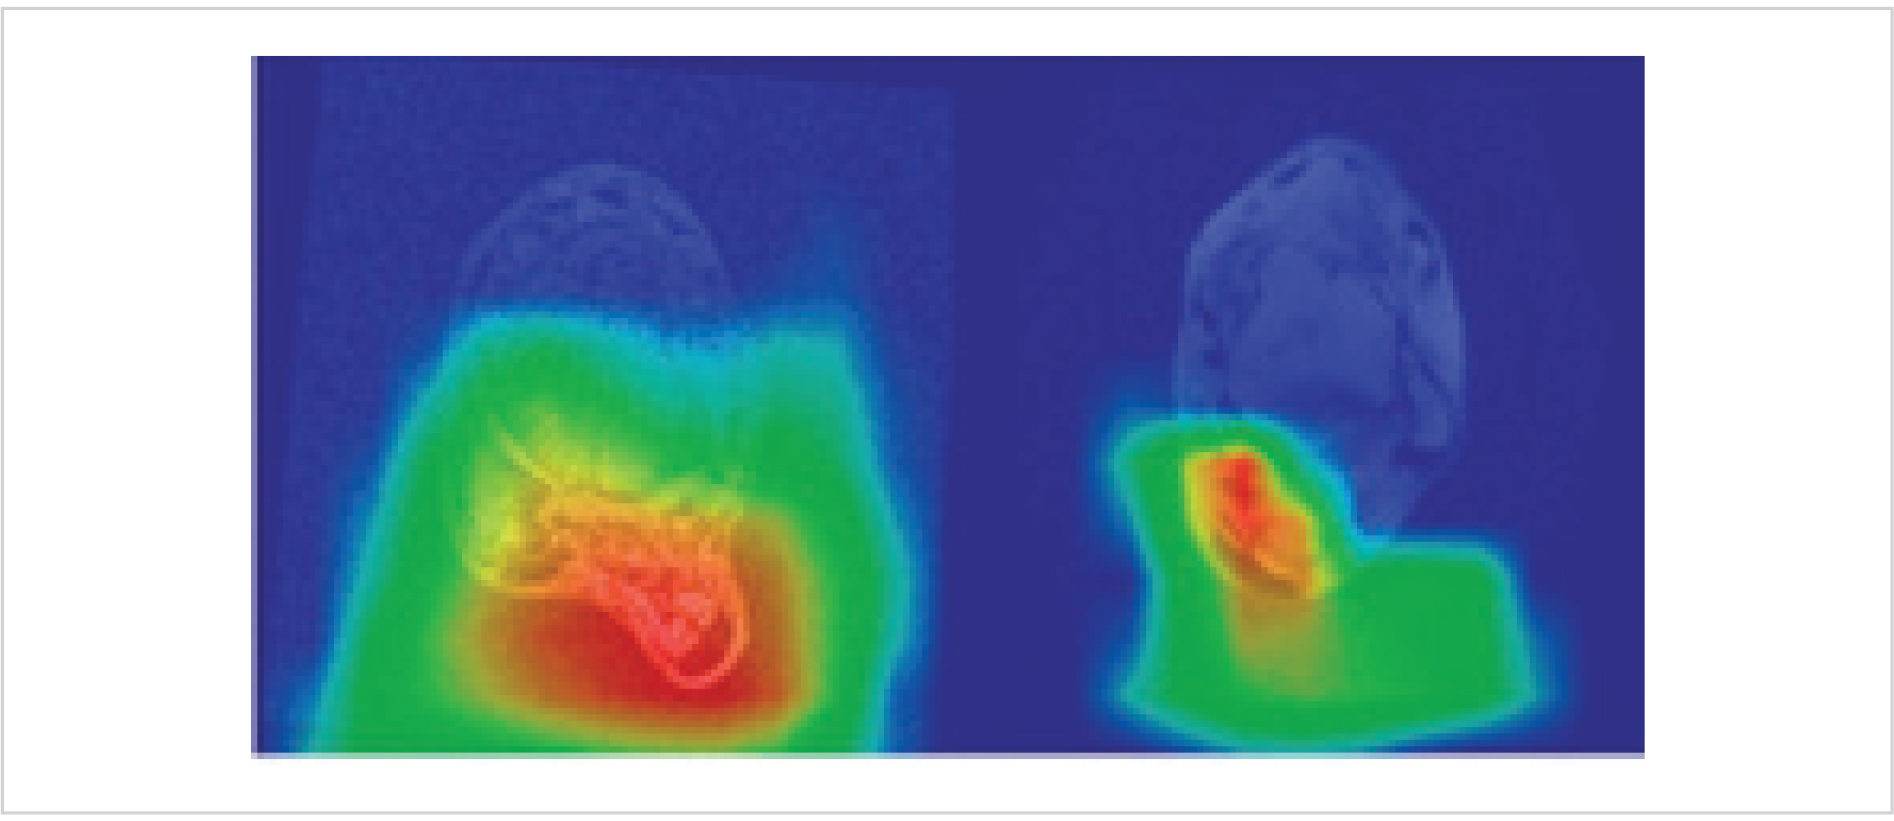
\includegraphics[width=1\textwidth]{figures/XAI.jpg}
	\caption{Analiza wizualna procesu wnioskowania sieci z zaznaczonym obszarem zainteresowania.}\label{fig:XAI}
\end{figure}
Można zaobserwować, że obszar zainteresowania wykorzystanej w eksperymentach sieci neuronowej obejmuje ROI jak i tkanki okalające. W celu zilustrowania zmian w czasie, na Rys. \ref{fig:3DXAI} pokazano izopowierzchnie przechodzące przez granicę obszaru zainteresowania w trójwymiarowych badaniach.
\begin{figure}[]
	\centering
	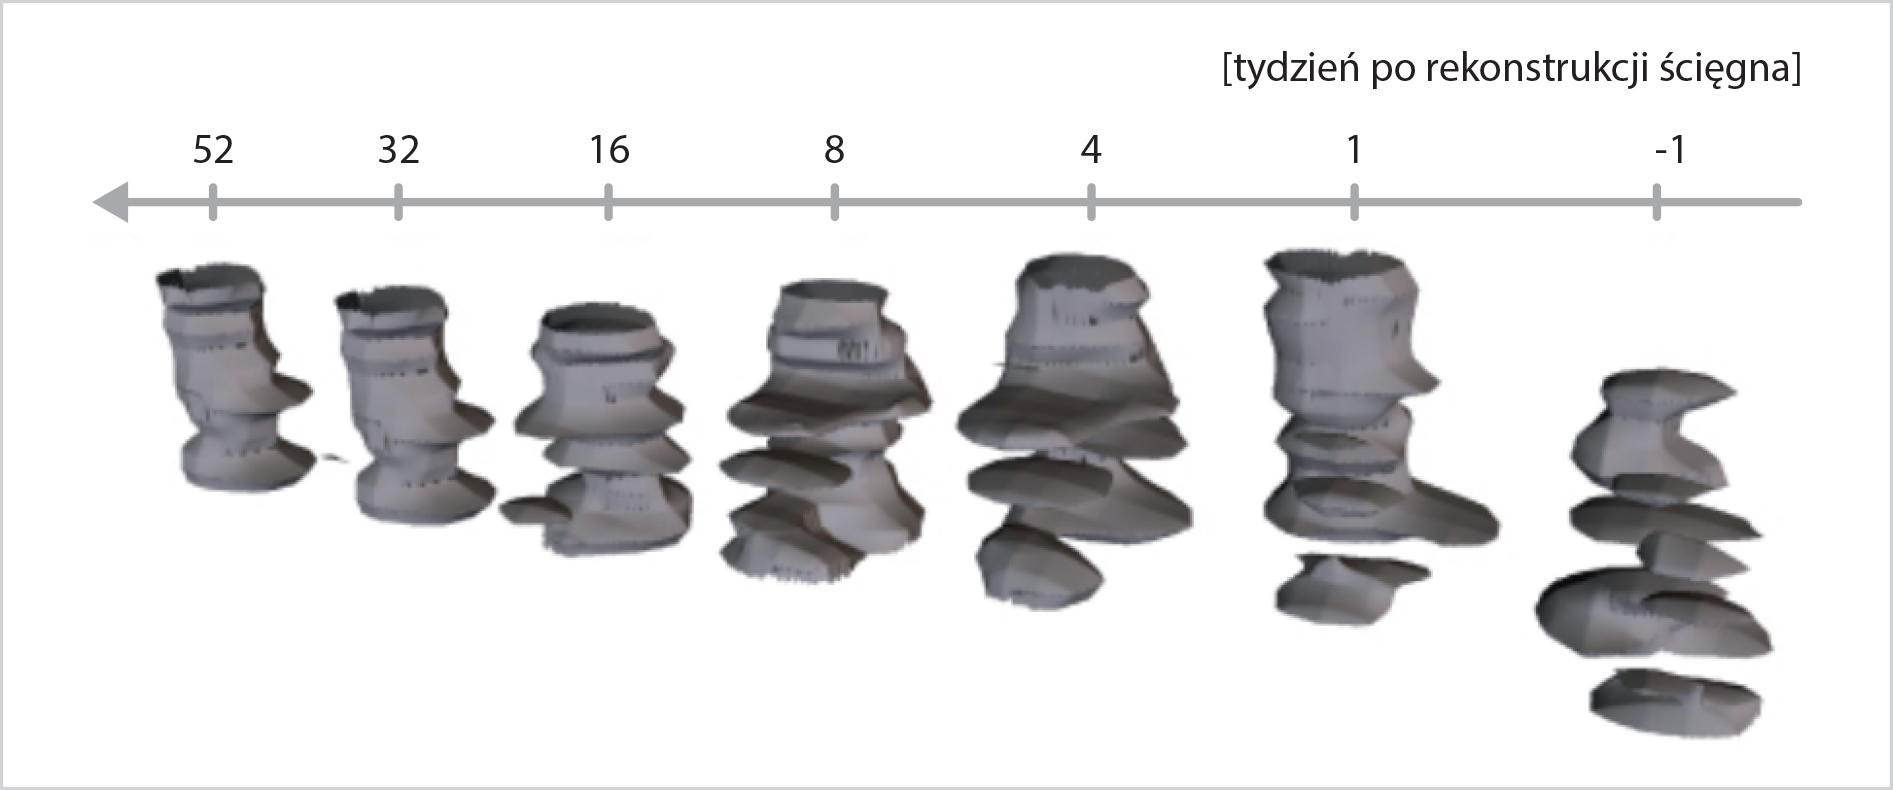
\includegraphics[width=1\textwidth]{figures/3DXAI.jpg}
	\caption{Trójwymiarowa wizualizacja zmian obszaru zainteresowania w kolejnych etapach gojenia się ścięgna.}\label{fig:3DXAI}
\end{figure}
Początkowo cechy w kolejnych przekrojach na podstawie, których wnioskuje sieć znajdują się w większym rozrzuceniu niż na końcu monitorowanego etapu gojenia się ścięgna.

Podsumowując, optymalna fuzja cech z widocznego obszaru ocenianego przez sieć neuronową oraz ROI umożliwia bardziej skuteczną ocenę całego procesu poprzez zapewnienie zgrubnej oceny z użyciem sieci i szczegółowej, z dołączenia predyktorów z ROI, bardziej odpornej na szum. 

\section{Ocena procesu gojenia}
\label{seq:valuation}
W ramach tego eksperymentu zostanie przedstawiona szczegółowa analiza wyników oceny procesu gojenia z wykorzystaniem proponowanej w tej pracy metody. \linebreak W pierwszej kolejności dokonano zgrubnej analizy. Przeanalizowano macierze błędu dla rożnych klas: (1) tygodni oceny, gdzie wartością jest średni błąd absolutny (MAE); (2) zakresu oceny (0--7), gdzie wartością jest liczba występowań. Następnie zostały przedstawione \textit{krzywe gojenia} tj. ocena zmiany w czasie poszczególnych parametrów ankiety. Porównane zostały szczegółowo, dla wszystkich testowych pacjentów, wyniki metody automatycznej z wzorcem odniesienia (ang. \textit{ground-truth}) tj. oceną eksperta radiologa.

\subsection{Macierze błędu}

Celem zdefiniowania ogólnych różnic między oceną radiologa i propozycją automatycznej metody, zestawiono dwa rodzaje macierzy błędu. W pierwszej kolejności jako klasę wybrano tydzień gojenia się ścięgna. Wyniki uzyskane z użyciem metody automatycznej porównano z oceną radiologa wykorzystując miarę średniego błędu absolutnego. Do obliczeń wykorzystano pacjentów testowych. Oddzielnie dla wszystkich 6-ciu parametrów wyznaczono macierze błędu i przedstawiono je na Rys.~\ref{fig:CM_MAE}. 

Z wykorzystaniem macierzy w stosunkowo łatwy sposób można określić w jakim stopniu wyniki ocen w poszczególnych tygodniach są do siebie zbliżone. \linebreak W przypadku możliwie najlepszego odwzorowania oceny radiologa przez nową metodę, minimalne błędy znajdowałyby się na diagonali przedstawionych wykresów. Dla poszczególnych parametrów można jednak zaobserwować dryf wartości minimalnych błędów. Pole powierzchni ($PP_d$) pomiędzy krzywą określającą wartości minimalne MAE a diagonalą zostały zebrane w Tabeli \ref{tab:dryf_meas}.
\vspace{10px} 
\begin{table*}[h!]
	\caption{Ocena dryfu krzywej łączącej minima lokalne wartości MAE w macierzach błędów z klasą przyjętą jako tydzień rehabilitacji.}
	\begin{center}
		\begin{tabular}{l||c|c|c|c|c|c}
		
			& \textbf{SCT} & \textbf{TT} & \textbf{STE} & \textbf{TE} & \textbf{TU} & \textbf{TisE}\\ 
			\hline \hline
			$PP_d$ &18&10&42&13&30&17\\	
					
		\end{tabular}
	\end{center}
	\label{tab:dryf_meas}
\end{table*}

\begin{figure}[]
	\centering
	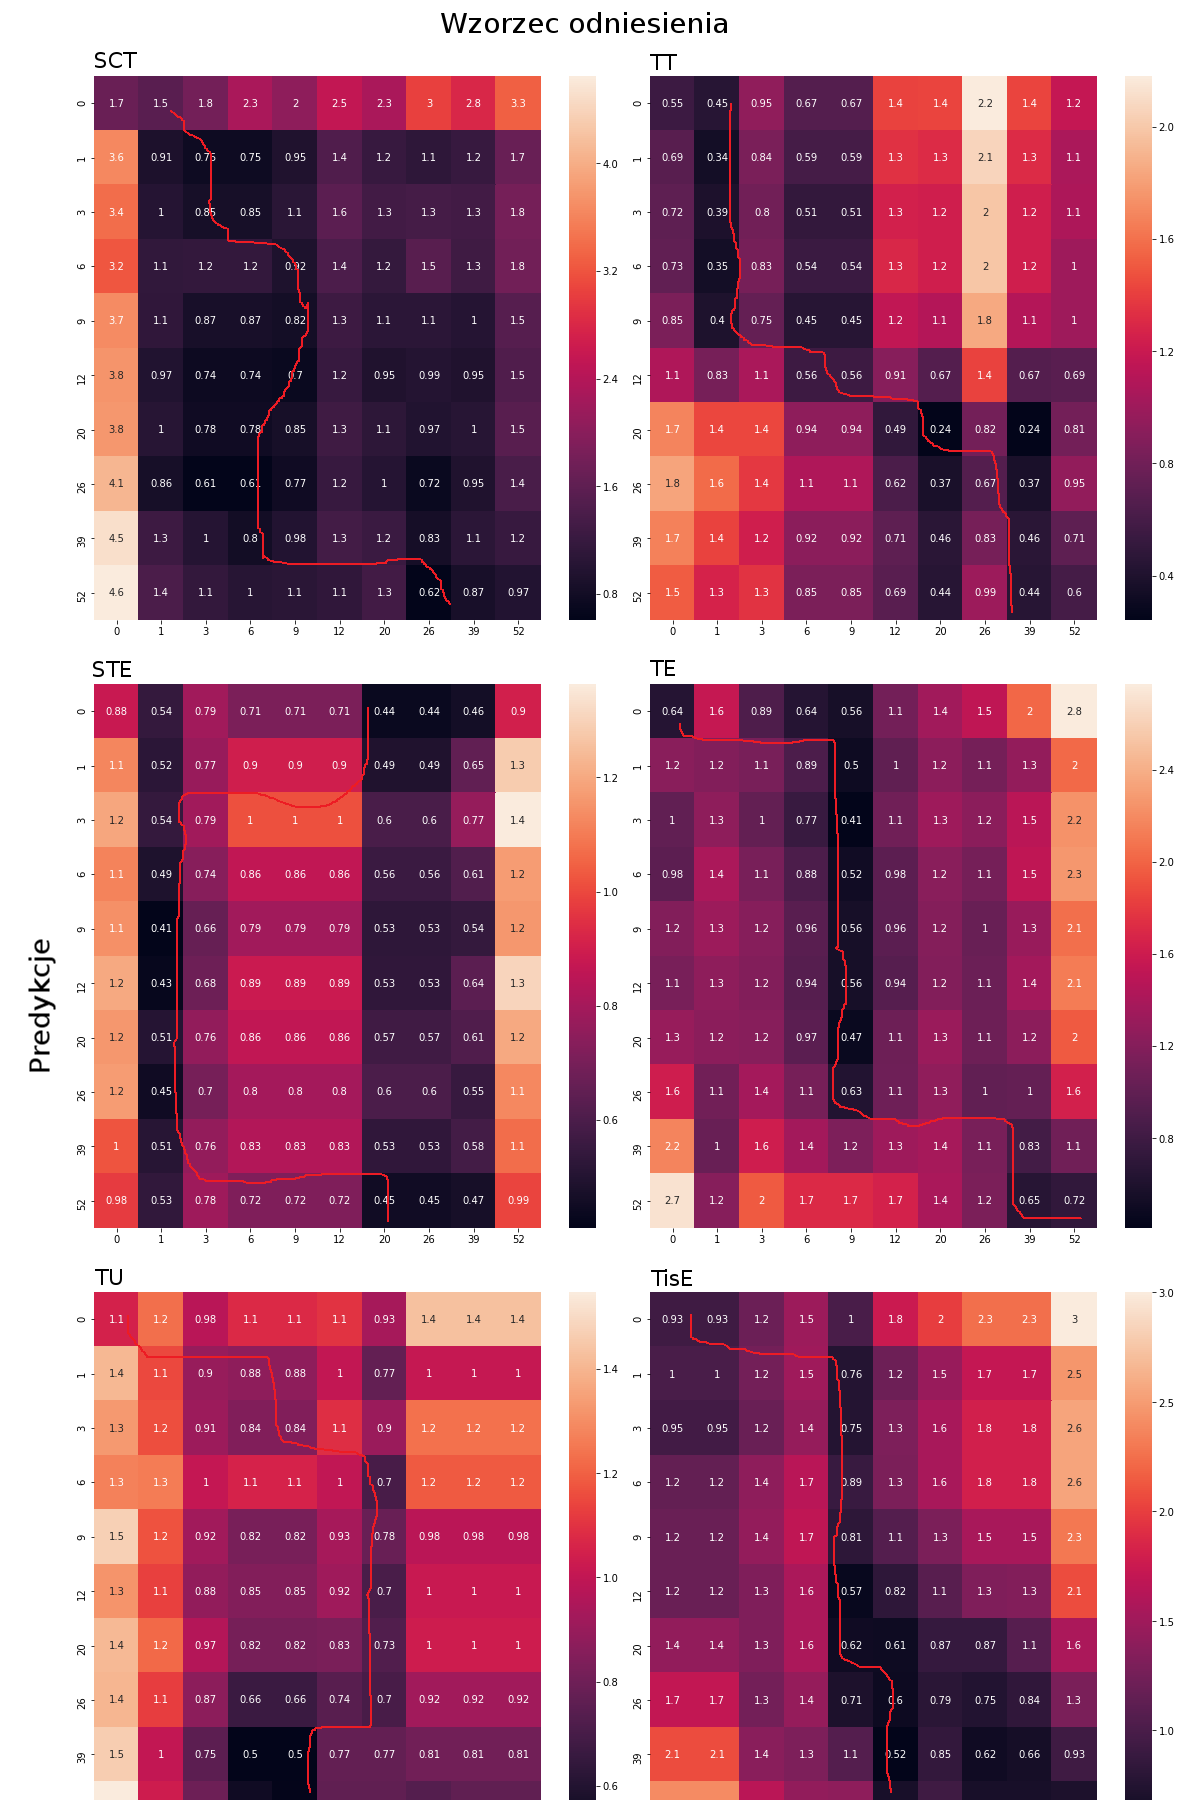
\includegraphics[width=0.9\textwidth]{figures/cm.png}
	\caption{Macierz średniego błędu absolutnego dla oceny pacjentów testowych.}\label{fig:CM_MAE}
\end{figure}
\newpage
Najlepsze rezultaty (najmniejszy $PP_d$) uzyskano dla parametru TT, a najgorszy dla STE, co oznacza, że w tych przypadkach ocena automatyczna najlepiej \linebreak i najgorzej przypomina ocenę radiologa. Kolejne, najlepsze rezultaty otrzymano dla parametrów opisujących obrzęki tj. TE i TisE oraz spójność ścięgna (SCT). Drugi najgorszy wynik został uzyskany dla parametru TU oceniającego jednorodność ścięgna w płaszczyźnie strzałkowej. Powyższe rezultaty są spójne z wnioskami \linebreak do wyników zamieszczonych w Tabeli \ref{tab:testset}, jednak szczegółowa analiza dryfu tydzień po tygodniu przedstawiono na Rys. \ref{fig:CM_MAE_SUMMARY} umożliwia dalsze wnioskowanie.

\begin{figure}[h]
	\centering
	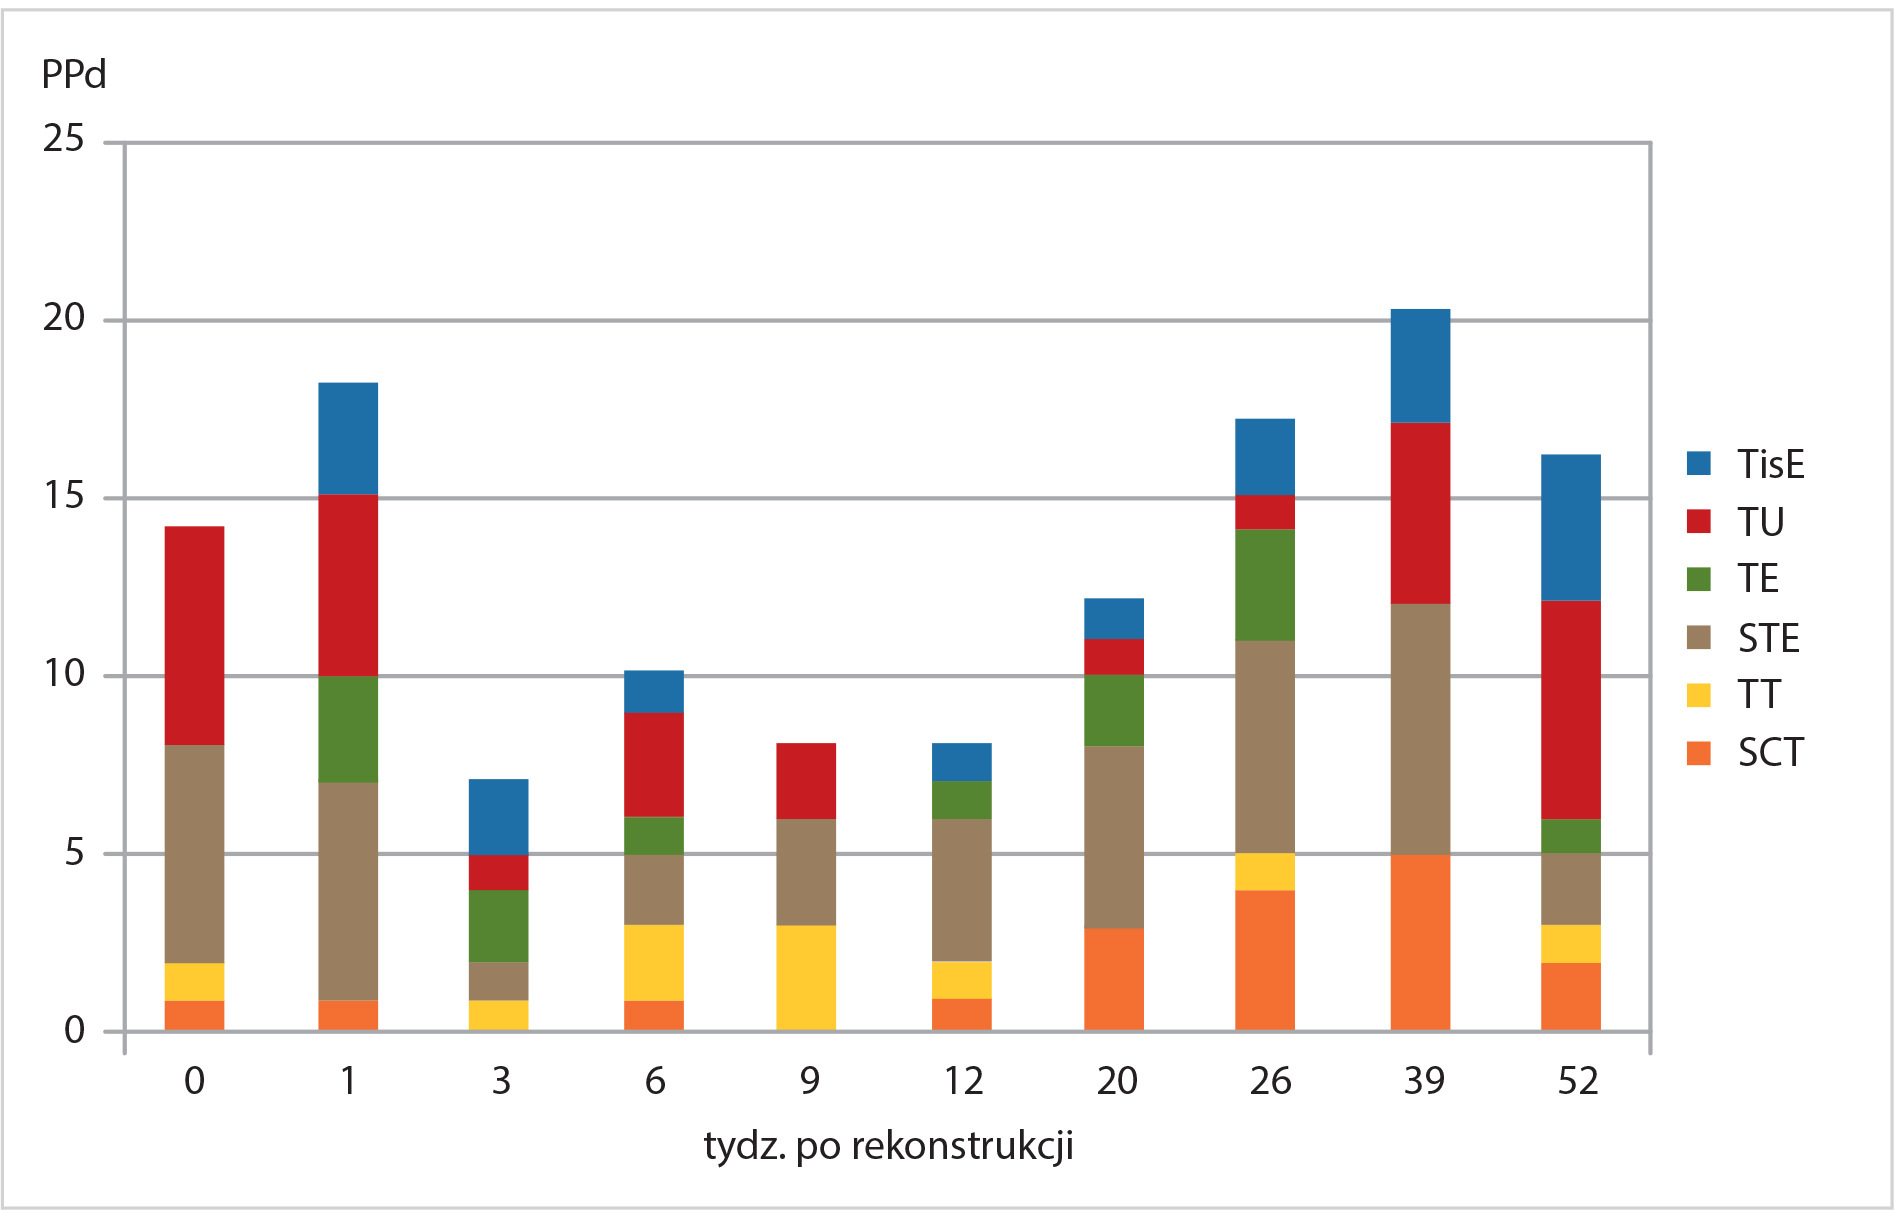
\includegraphics[width=1\textwidth]{figures/cm_summary.jpg}
	\caption{Wartości $PP_d$ dla parametrów z wzorca odniesienia.}\label{fig:CM_MAE_SUMMARY}
\end{figure}

Najmniejsze różnice w ocenie występują w trzecim tygodniu, czyli w pierwszym pomiarze po fazie zapalnej. Natomiast, wyróżniające dwie największe są obecne \linebreak w pierwszym oraz 39-tym tygodniu monitoringu, zatem w szczycie fazy zapalnej \linebreak i w momencie zaawansowania fazy przebudowy. 

Analizując poszczególne parametry od najlepszego pod względem $PP_d$: w przypadku parametru TT, największe różnice w ocenie widoczne są między 3--12 tyg., \linebreak a zatem na przełomie fazy poliferacji i przebudowy, gdzie włókna ścięgniste zaczynają się ukierunkowywać i zmienia się grubość ścięgna. Dla TE największe odchylenia zaobserwowano dla przełomu fazy zapalnej i poliferacji -- tydz. 1 oraz zaawansowanej przebudowy w 26-tym tyg. Podobny schemat zachowany jest dla TisE, \linebreak z tą różnicą, że oprócz przełomu fazy zapalnej, odchylenia są widoczne w całym okresie przebudowy. Może to świadczyć o różnicy w ocenie płynów nagromadzonych w obrzękach. W przypadku SCT, różnice w ocenie spójności włókien uwidaczniają się w fazie przebudowy, kiedy to automatyczna metoda nie wskazuje na znaczący postęp w stosunku do wyniku z 26-tego tygodnia. W przypadku dwóch parametrów uzyskujących najgorszy wynik $PP_d$ tj. TU i STE rozbieżności są widoczne \linebreak w całym okresie monitoringu, w szczególności w fazie zapalnej i przebudowy. Faza zapalna jest najbardziej dynamiczna, natomiast faza przebudowy była monitorowana w najdłuższych interwałach, co może powiększać różnice w obrazach tkanek \linebreak w obu przypadkach. 

Do dalszej analizy różnic między ocenami wykorzystano macierze błędu, gdzie klasą jest nota przyznawana w ocenie parametrów (zob. Rys. \ref{fig:cmscores}).
\begin{figure}[h]
	\centering
	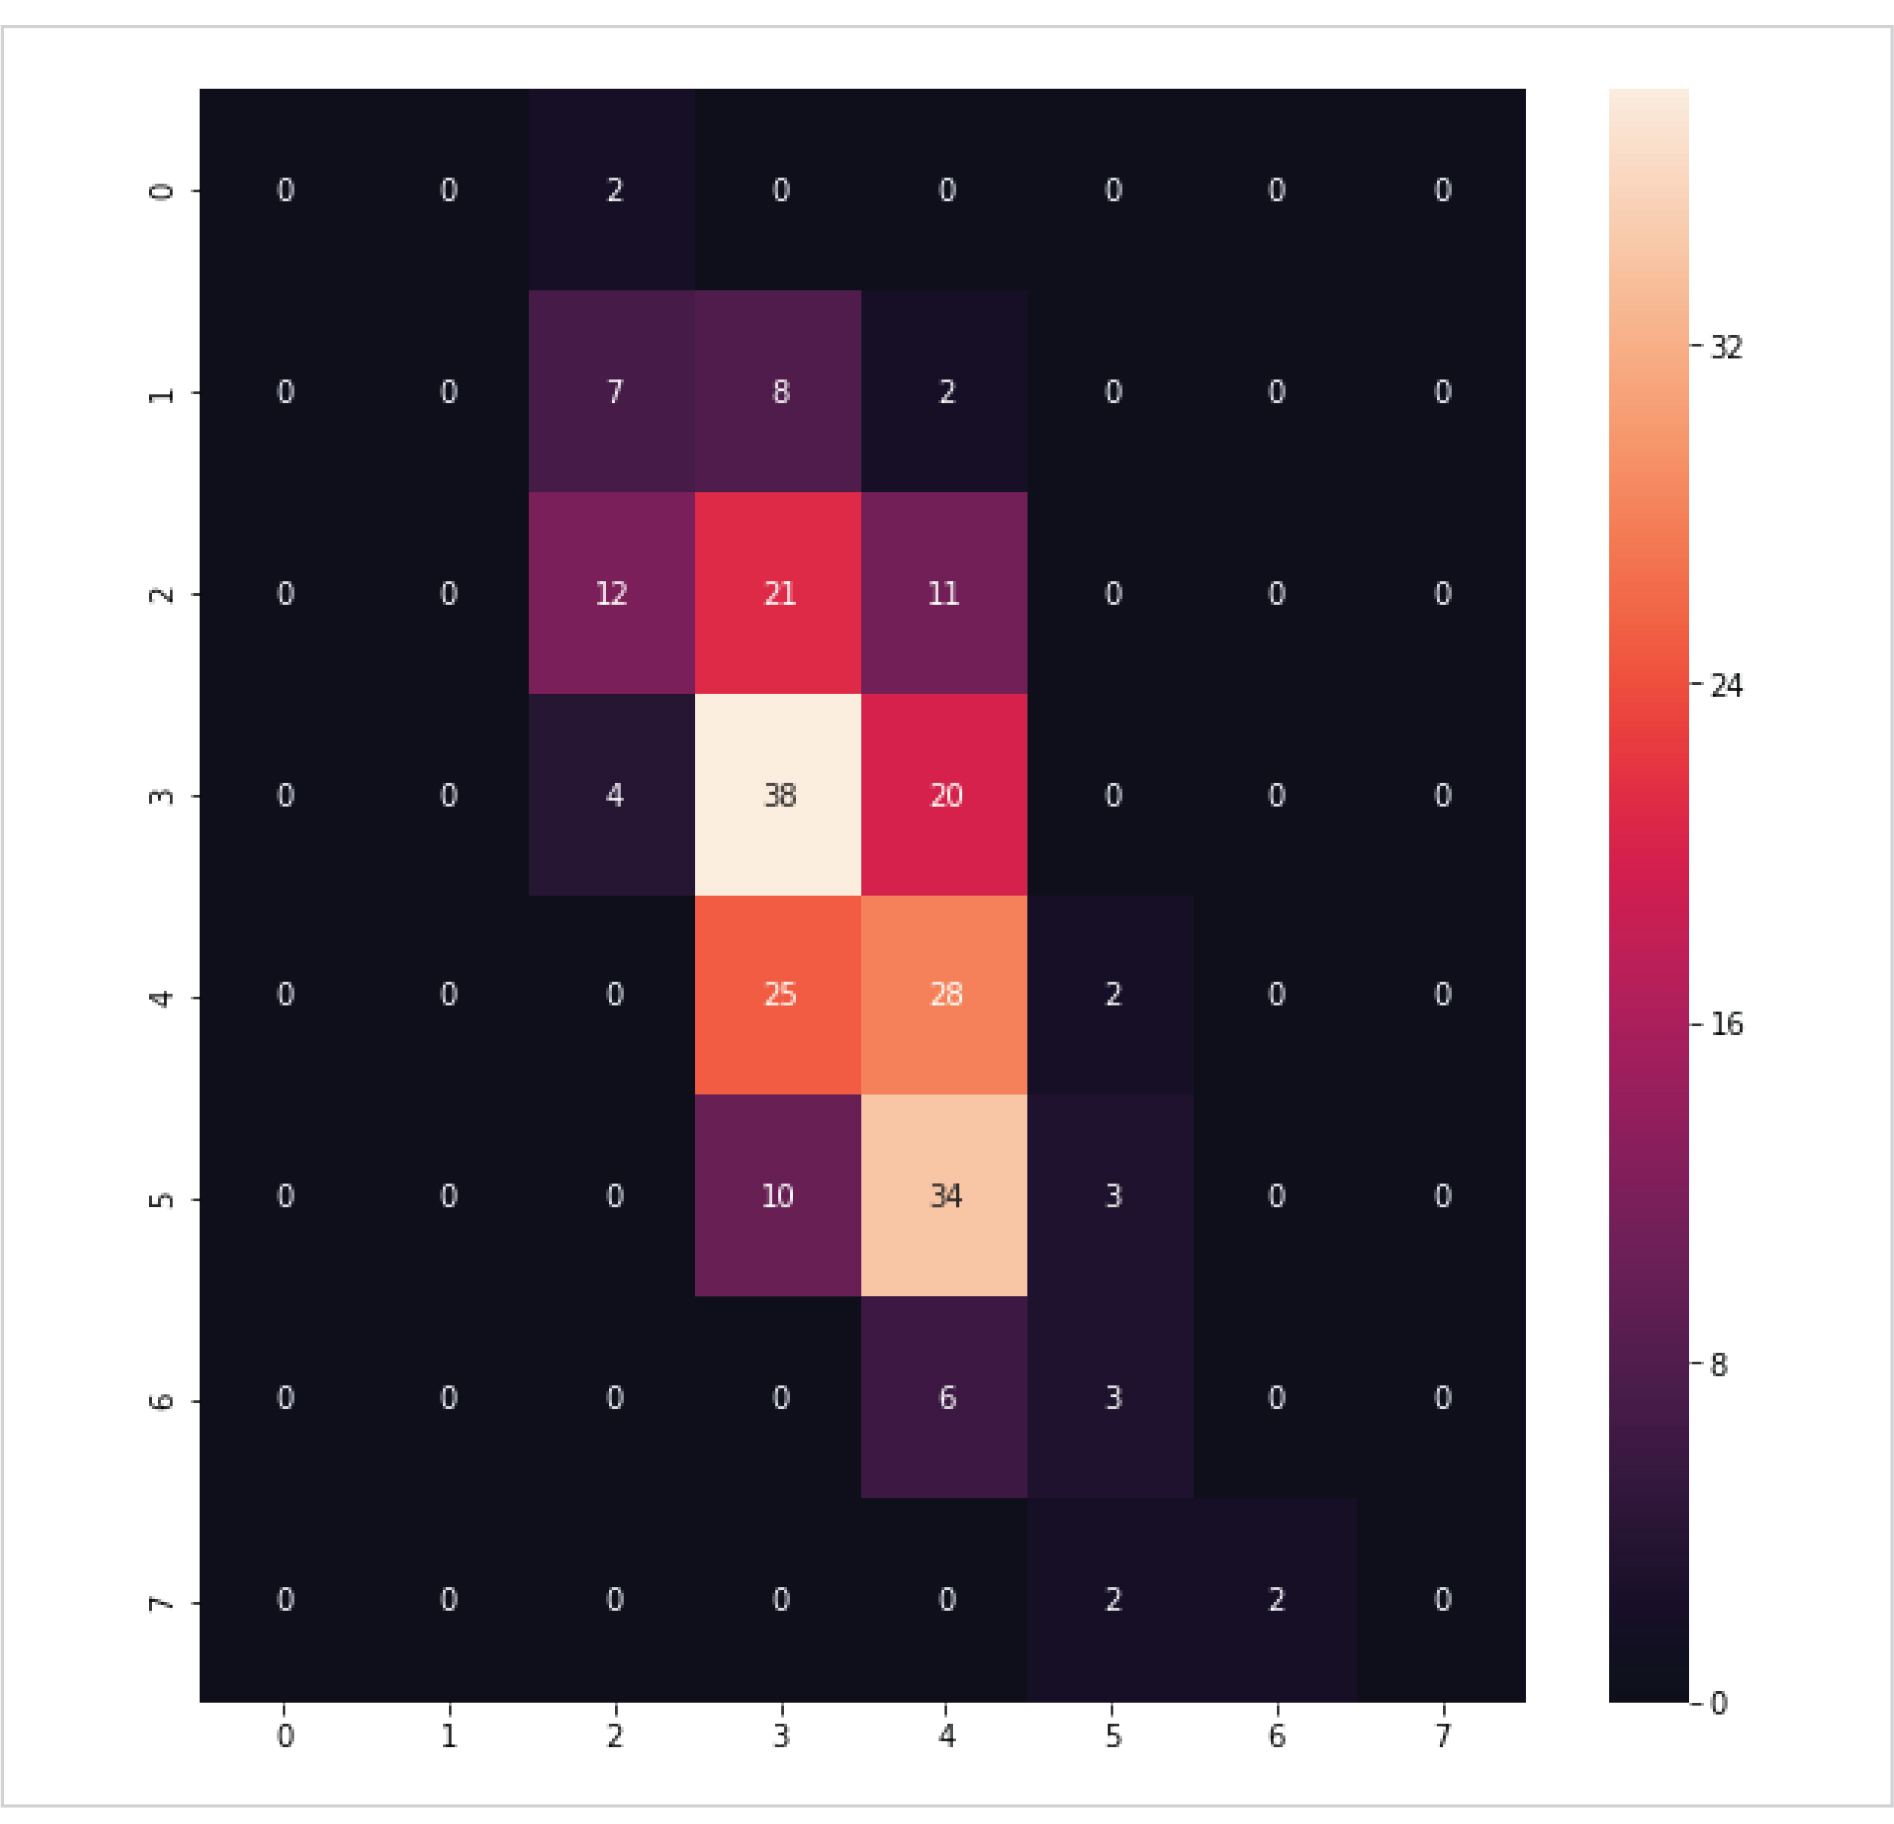
\includegraphics[width=0.9\textwidth]{figures/cmScores.jpg}
	\caption{Macierz błędu dla noty jako klasy.}\label{fig:cmscores}
\end{figure}

Największą zgodność otrzymano dla 2, 3 i 4. Notę 5 najczęściej automatyczna metoda oceniła jako 4, podobnie jak notę 6. Notę 7, dwukrotnie oceniona została jako notę 5 albo 6. W przypadku niskich wyników oceny, 1 najczęściej wystąpiła jako nota 2 (7 razy) lub 3 (8 razy). Natomiast nota 0 wystąpiła jako 2. Wartości błędów dla poszczególnych tygodniach przedstawiono na Rys. \ref{fig:cmscores_summary}.

\begin{figure}[h]
	\centering
	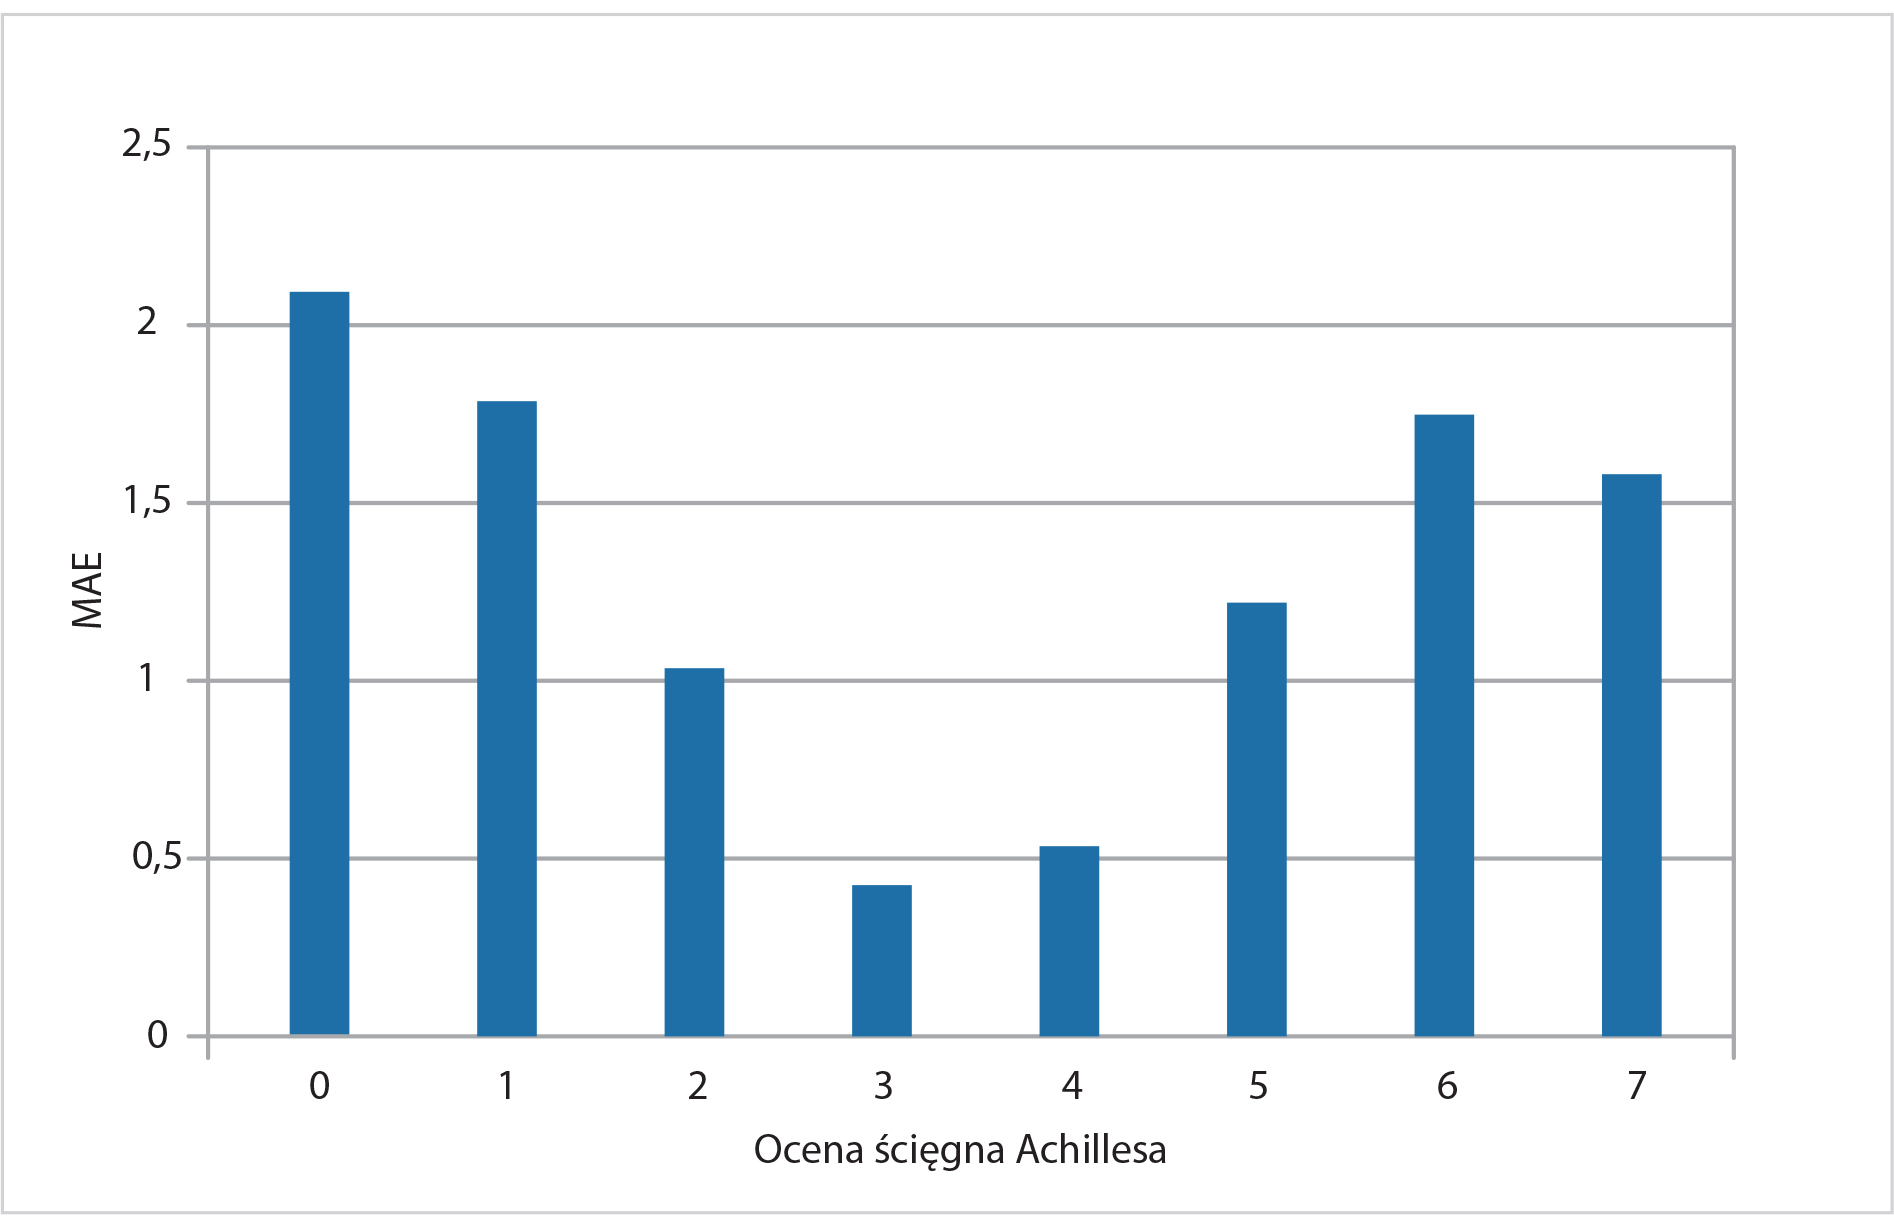
\includegraphics[width=1\textwidth]{figures/cmScores_summary.jpg}
	\caption{MAE w obrębie klas.}\label{fig:cmscores_summary}
\end{figure}

Można zaobserwować, że najmniejsze błędy ($<$1) otrzymywane są w zakresie not 2--4. Dla noty 5 wynik jest nieznacznie gorszy i osiąga poziom MAE=1,15. \linebreak W pozostałych notach skrajnych błąd wynosi $>$ 1,5. Wyniki są związane z faktem, że metoda automatyczna charakteryzuje się mniejszym zakresem oceny, co wynika z zastosowania w algorytmie meta-regresji. Wartości oceny nigdy nie osiągają not skrajnych tj. 7 lub 0--1. 

\subsection{Krzywe gojenia}
 Dla czterech pacjentów testowych, dla każdego z dziesięciu kroków czasowych, zestawiono wyniki oceny automatycznej z oceną eksperta radiologa. Na kolejnych sześciu rysunkach zaprezentowano rezultaty dla wszystkich parametrów z ankiety. Jako pierwszy przedstawiono parametr SCT (zob. Rys. \ref{fig:SCT}).
\begin{figure}[h!]
	\centering
	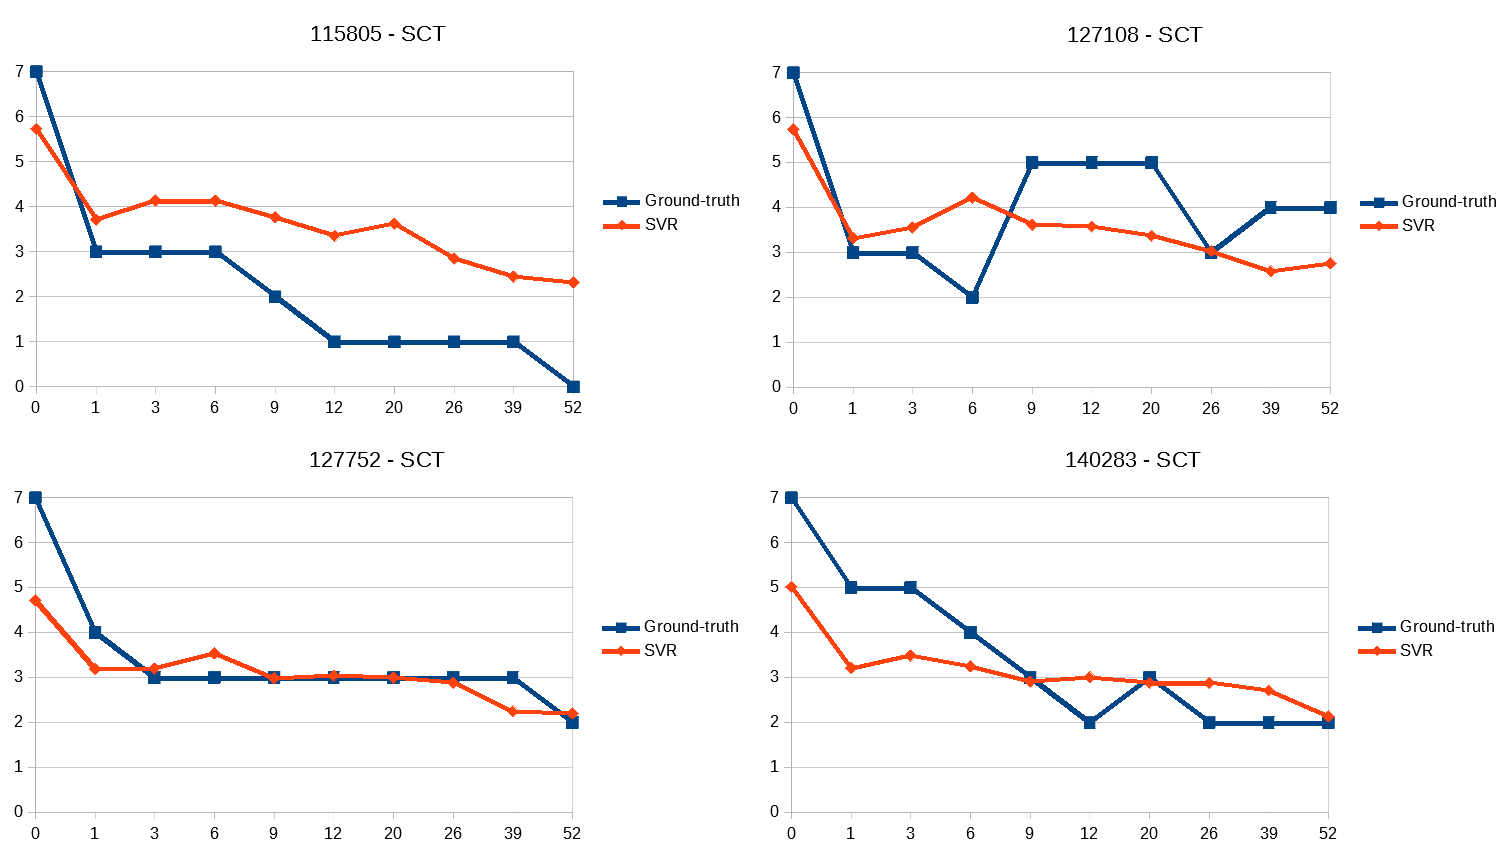
\includegraphics[width=1\textwidth]{figures/SCT.png}
	\caption{Ocena parametru SCT.}\label{fig:SCT}
\end{figure}

Zgodnie z opisem zamieszczonym w p. \ref{seq:ground-truth} dotyczy on stanu uszkodzeń śródścięgnistych wewnątrz obszaru ROI. Przed interwencją chirurgiczną ścięgno jest całkowicie zerwane, stąd w tygodniu 0, reprezentującym czas na kilka dni przed operacją, ocena radiologa wynosi 7, dla każdego z pacjentów. Po zszyciu w 3-ech z 4-ech przypadkach, proces postępuje z malejącym trendem do osiągnięcia małych, bądź braku uszkodzeń (jedyna anomalia, mogąca wynikać z omawianych wcześniej czynników zaburzających proces gojenia się, widoczna jest w 20-tym tyg. dla pacjenta 140283). W przypadku pacjenta 127108 proces gojenia się jest odmienny, przebiega z wyraźnie zmiennym trendem, jak również kończy się oceną 4, interpretowaną jako dość duże uszkodzenia. Ocena automatyczna proponowana w tej pracy przybliża trendy oceny radiologa, sugerując duże lub bardzo duże uszkodzenia na początku procesu i małe uszkodzenia w 3-ech z 4-ech przypadkach na końcu. Jedynie dla pacjenta 127108 sugerowana nota końcowa oznacza uszkodzenia średniej wielkości. Poza pojedynczym maksymalnym błędem (MAX-AE) występującym w 20-tym tyg. w ocenie pacjenta 115805, największe obserwowalne różnice w ocenie występują przed operacją. \linebreak We wszystkich czterech przypadkach ocena automatyczna stanu ekstremalnie dużych uszkodzeń związanych z całkowitym zerwaniem nie występuje, co wynika z ogólnie mniejszego zakresu punktacji metody automatycznej. 

Kolejnym analizowanym parametrem jest TT. Wykresy krzywych gojenia przedstawiono na Rys. \ref{fig:TT}.    
\begin{figure}[h!]
	\centering
	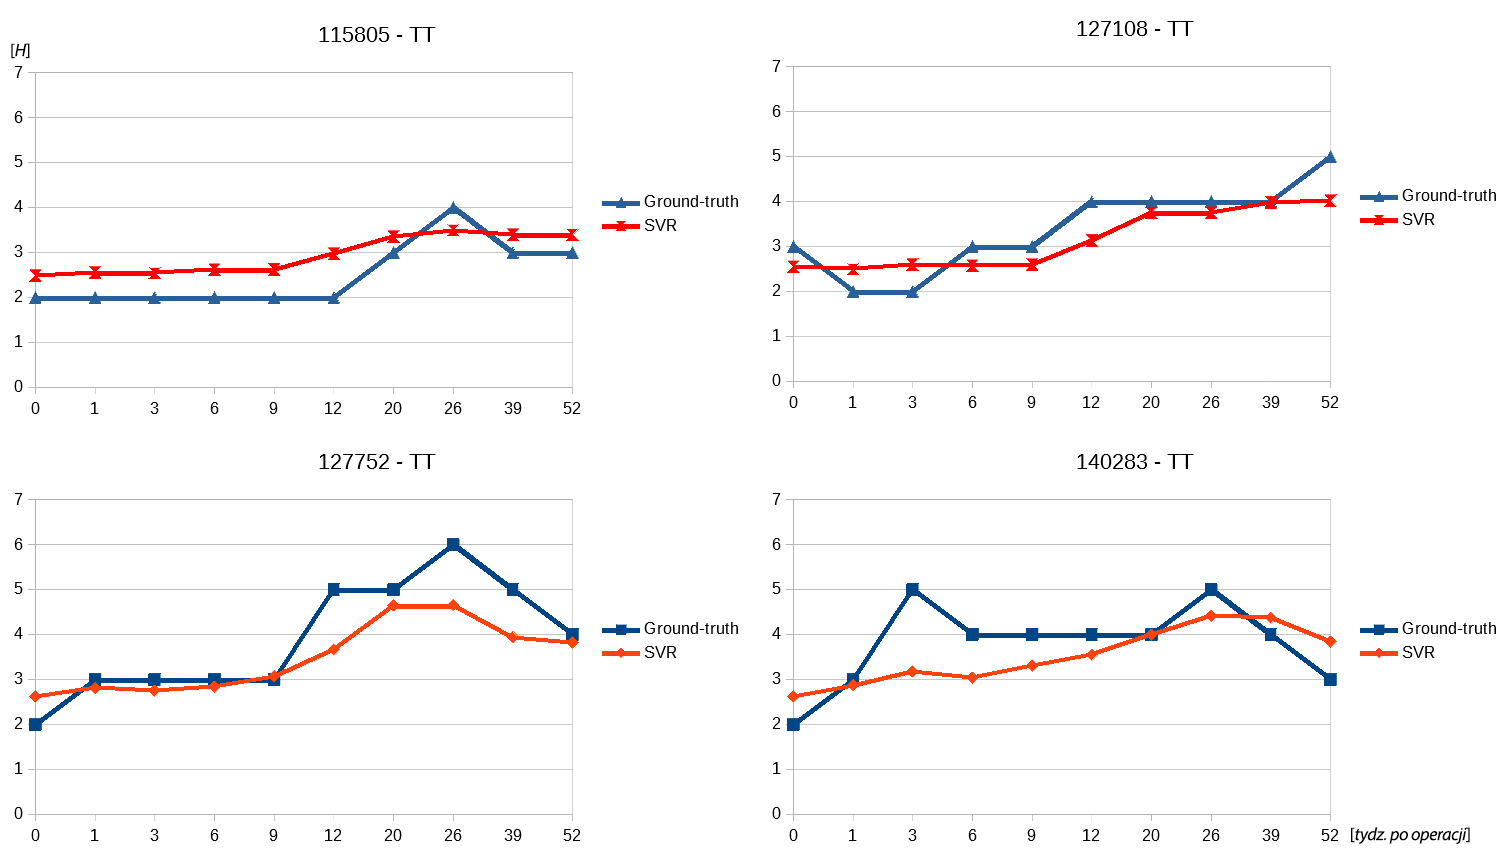
\includegraphics[width=1\textwidth]{figures/TT.png}
	\caption{Ocena parametru TT.}\label{fig:TT}
\end{figure}
Parametr ten zgodnie z przedstawioną interpretacją związany jest z oceną pogrubienia ścięgna. Na początku procesu pogrubienie jest małe lub średnie (9--12 mm.), następnie w fazie poliferacji i początkach przebudowy rośnie, co związane jest z przyrostem włókien ścięgnistych, by finalnie, w większości przypadków, ponownie zmaleć w wyniku przebudowy struktury i pozostawienia jedynie dobrze ukierunkowanych, wytrzymałych struktur. Dla pacjentów 115805 \linebreak i 127752, w ocenie radiologa proces przebiega zgodnie z wyżej przedstawionym opisem. W przypadku pacjenta 140283 widoczna jest anomalia w 3-ecim tyg., co może mieć związek z fluktuacjami np. nadmiernym obciążeniem ścięgna. Ponownie, jedynie w przypadku pacjenta 127108, gojenie przebiega odmiennie i po operacji pogrubienie rośnie, aż do 52-ego tyg. 

Błąd (MAE), równy 0,56, osiągnięty dla oceny tego parametru jest najniższy spośród wszystkich sześciu, co widoczne jest w przebiegach krzywych gojenia, które dobrze przybliżają ocenę radiologa. Anomalia w 3-ecim tyg. występująca u pacjenta 140283 nie została dobrze wykryta i w rezultacie błąd maksymalny (MAX-AE) wyniósł 1,82. W celu detekcji przyczyny konieczna jest dalsza analiza i w pierwszej kolejności weryfikacja, czy błąd popełniony został przez ocenę radiologa, czy metodę.

Następnym analizowanym parametrem jest STE. Wykresy krzywych gojenia przedstawiono na Rys. \ref{fig:STE}.
\begin{figure}[h!]
	\centering
	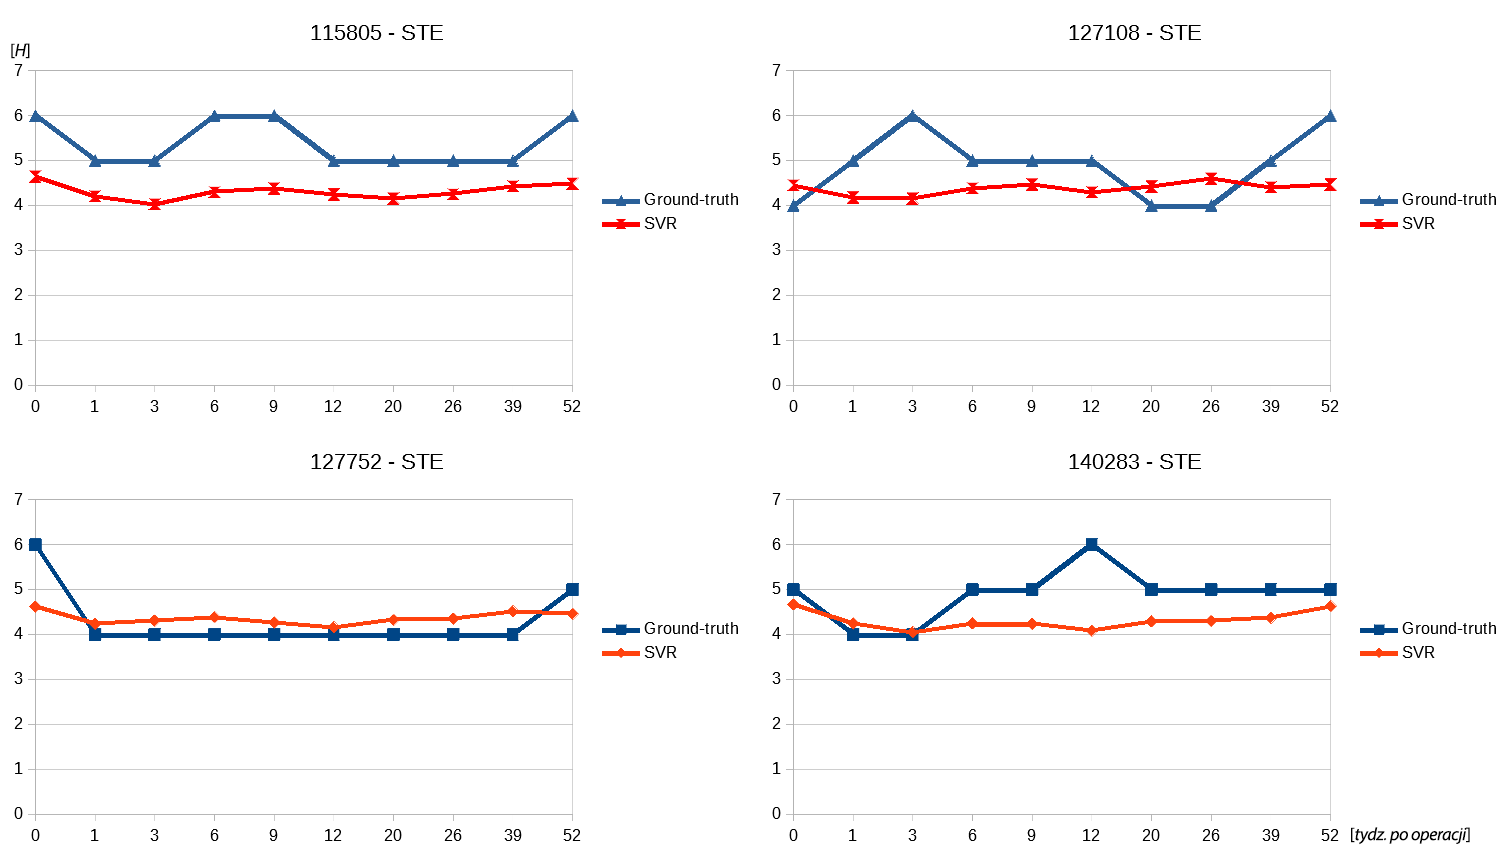
\includegraphics[width=1\textwidth]{figures/STE.png}
	\caption{Ocena parametru STE.}\label{fig:STE}
\end{figure}
Parametr ten związany jest z oceną granic pomiędzy ROI, a zewnętrznymi tkankami. Ścięgno po zerwaniu nigdy nie odzyskuje zdrowych granic, stąd ocena radiologa oscylująca w zakresie 4--6. Zakres oceny automatycznej jest jeszcze mniejszy i wynosi po zaokrągleniu 4--5. Skutkiem tak niskich zakresów jest najgorszy wynik miary Corr spośród wszystkich sześciu parametrów, co oznacza, że drobne zmiany krawędziowe nie są dobrze oceniane przez proponowaną metodę automatyczną. Z uwagi na mały zakres zmian, MAE i MAX-AE osiągnęły drugi najlepszy wynik. Na tym etapie informatywność tego parametru pozostaje wątpliwa i konieczna jest dalsza weryfikacja.

Jako czwarty parametr przedstawiono TE. Uzyskane krzywe gojenia zaprezentowano na Rys. \ref{fig:TE}.
\begin{figure}[h!]
	\centering
	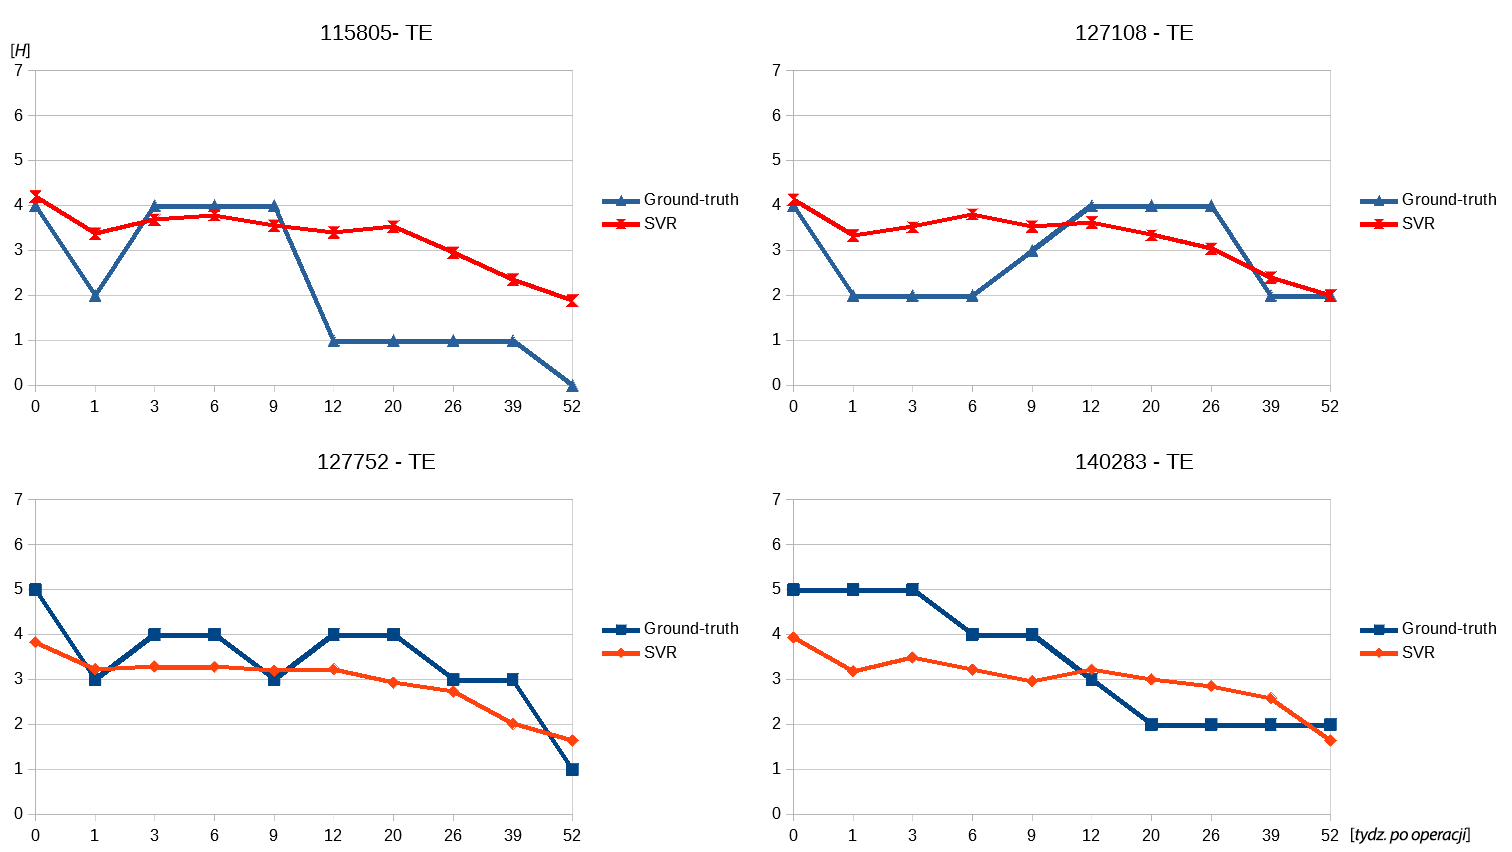
\includegraphics[width=1\textwidth]{figures/TE.png}
	\caption{Ocena parametru TE.}\label{fig:TE}
\end{figure}
W tym przypadku ocena radiologa skupiona jest na analizie płynów gromadzących się w obszarze ROI, powodujących jego obrzęk. W większości przypadków, zszycie ścięgna powoduje redukcję płynów w ROI, które następnie \linebreak w wyniku intensywnych procesów zapalnych i budowy nowych włókien ulegają ponownej akumulacji. W ostatniej fazie przebudowy, z uwagi na zmniejszenie intensywności procesów, objętość płynów ponownie jest redukowana. Dla wszystkich czterech pacjentów ocena radiologa oddaje powyższy opis. W przypadku pacjenta 127108 można zaobserwować dłuższe fazy redukcji i akumulacji płynu, co ponownie potwierdza odmienność procesu gojenia dla tego przypadku. Interesujący jest przypadek pacjenta 140283, gdzie w tygodniu 1 po operacji minimum lokalne widoczne jest tylko w wyniku oceny automatycznej. W tym przypadku rozdzielczość skali radiologa okazała się być zbyt mała. Szukając powodów błędów maksymalnych, ponownie można wskazać jako podstawowy powód mniejszy zakres zmian oceny automatycznej. W 12 tyg. oceny pacjenta 115805 występuje silna redukcja obrzęku. W ocenie automatycznej widoczne jest lokalne minimum, ale jego wartość odbiega od wzorca o 2,48, a w następnym kroku o 2,52 osiągając MAX-AE. 

Przedostatnim z analizowanych parametrów jest TU. Krzywe gojenia zostały zaprezentowane na Rys. \ref{fig:TU}.  
\begin{figure}[h!]
	\centering
	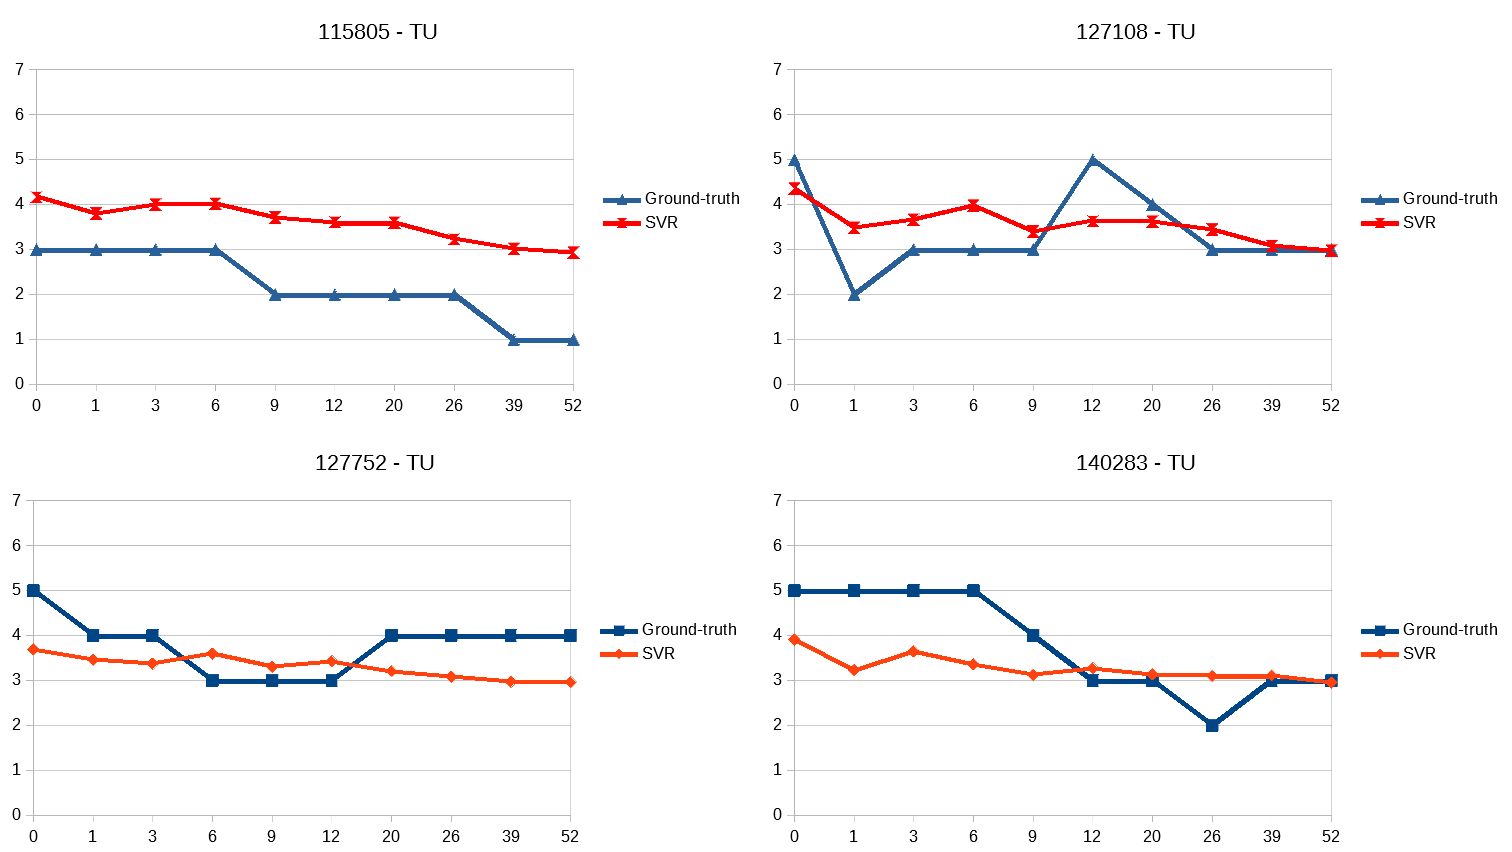
\includegraphics[width=1\textwidth]{figures/TU.png}
	\caption{Ocena parametru TU.}\label{fig:TU}
\end{figure}
Jest to jedyny parametr oceniany w całości w płaszczyźnie strzałkowej. Przy jego użyciu interpretowana jest jednorodność ścięgna widoczna w postaci charakterystycznego zdrowego warkocza włókien. Struktura \linebreak ta w procesie gojenia się ulega stopniowej poprawie, co odzwierciedlają oceny radiologa dla pacjentów 115805 i 140283 (z jedną anomalią w 26-tym tyg.). Dla pacjenta 127752 jednorodność ścięgna ulega pogorszeniu na przełomie 12-tego i 20-tego tyg., co może być wynikiem czynników zewnętrznych wpływających na przebieg gojenia. Natomiast krzywa dla pacjenta 127108 ponownie zawiera odmienne trendy, zwłaszcza na przełomie 9-tego i 12-tego tyg. Dla automatycznej oceny, parametr oceniany jest z drugim (zaraz po STE) najgorszym wynikiem pod względem Corr i również \linebreak z drugim, najgorszym MAE. Analiza automatyczna bazuje na metodzie wytrenowanej jedynie z wykorzystaniem przekrojów osiowych. Uzyskane wyniki są zatem efektem agregowanych w mierze $H$ wartości lub korelacji z innymi parametrami. 
\newpage
Jako ostatni został przeanalizowany parametr TisE. Charakteryzuje on obrzęk \linebreak w przestrzeni międzypowięziowej ścięgna Achillesa. Krzywe gojenia widoczne \linebreak są na Rys. \ref{fig:TisE}.
\begin{figure}[h!]
	\centering
	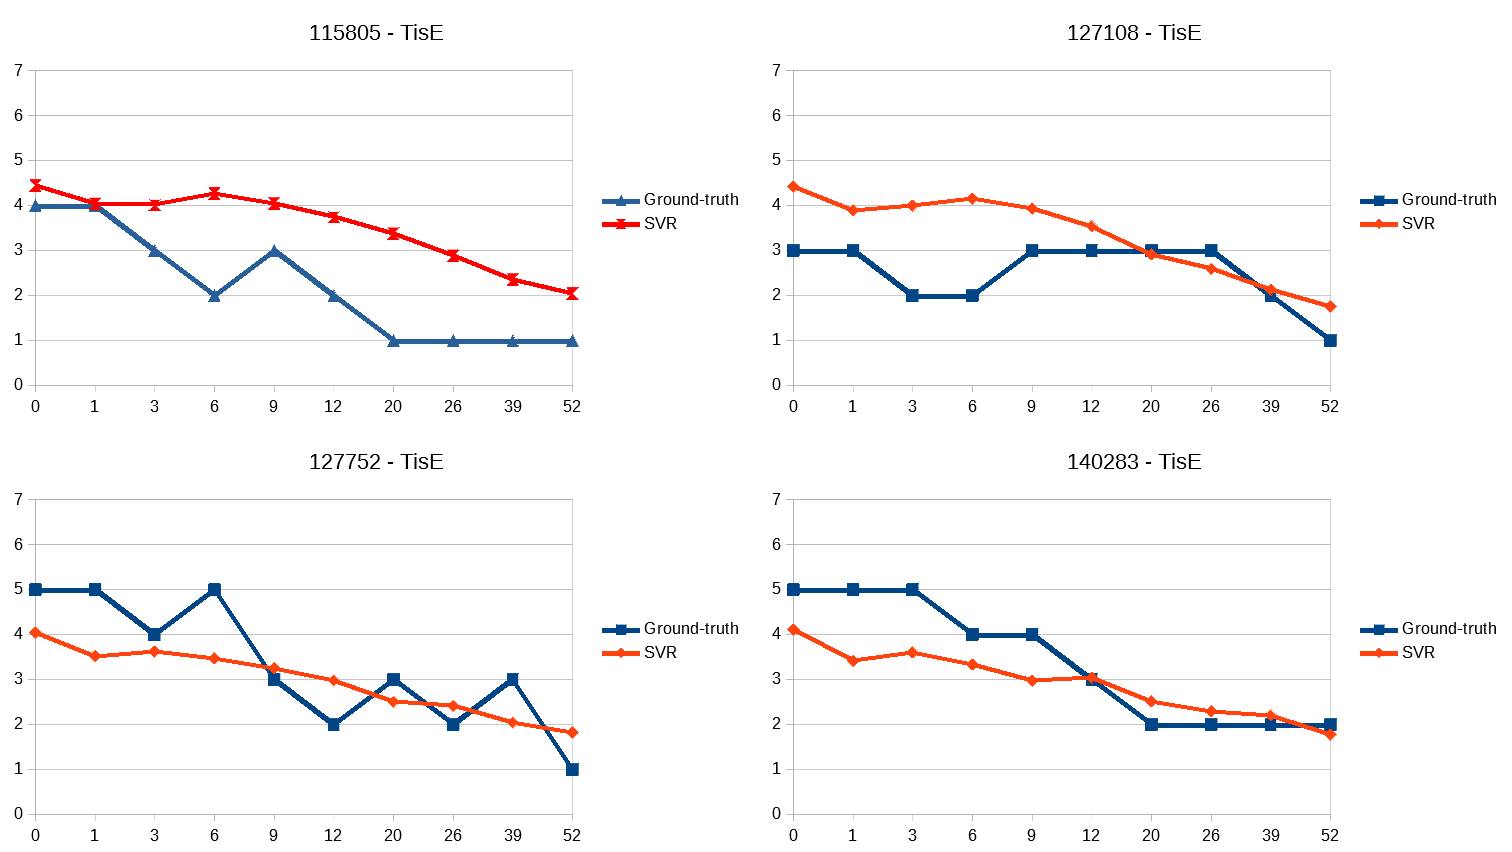
\includegraphics[width=1\textwidth]{figures/TisE.png}
	\caption{Ocena parametru TisE.}\label{fig:TisE}
\end{figure}
Jest to jedyny parametr oceniany w całości na zewnątrz ROI, tylko z wykorzystaniem cech DL. Na przełomie fazy poliferacji i remodelingu (tydz. 6--9) następuje charakterystyczny, krótkotrwały wzrost płynów w tym obszarze, wynikający z intensywności procesu. W ocenach radiologa, szczególnie widoczny jest on dla pacjenta 115805 i 127752. Dla pacjenta 140283 widoczna jest stagnacja, \linebreak a dla 127108 zwiększenie obrzęku, które utrzymuje się przez kolejne etapy do 26-tego tyg. W krzywych wygenerowanych w ocenie automatycznej widoczne są również maksima lokalne w okolicach przełomu faz gojenia się. Są one jednak przesunięte względem oceny radiologa (tydz. 3--6), co wymaga dalszej analizy.

\subsection{Ocena holistyczna}

W celu efektywnego porównania nowych zmiennych opisujących biomechanikę ścięgna i wyniku ATRS z predykcjami automatycznej metody oraz oceną radiologa, zdecydowano się również dla badań radiologicznych przeprowadzić analizę czynnikową. W obu przypadkach tj. oceny automatycznej i radiologa uzyskano minimalny udział w wyjaśnianej wariancji czynników innych niż pierwszy. Stąd możliwość wprowadzenia nowej zmiennej tj. Czynnik1 zamiast 6-ciu parametrów: SCT, STE, TE, TisE, TT, TU. Szczegółowe wyniki znajdują się w Tabeli \ref{tab:pca-gt-pred}.

\begin{table}[h]
	\centering
	\setlength{\tabcolsep}{3pt}
	\setlength\extrarowheight{2pt}
	\caption{Rezultaty analizy czynników głównych dla oceny radiologicznej i oceny automatycznej realizowanych z wykorzystaniem 6-ścio parametrycznej ankiety. Oznaczono ładunki, gdzie wartość modułu jest większa niż 0,7.}
	\label{tab:pca-gt-pred}
	\begin{tabular}{c|c|c}
		Zmienna&Czynnik1 - ocena radiologa&Czynnik1 - ocena automatyczna \\
		\hline \hline
		SCT&\textbf{-0,79}&\textbf{-0,95}\\
		\hline
		STE&0,57&\textbf{0,86}\\
		\hline
		TE&\textbf{-0,85}&\textbf{-0,94}\\
		\hline
		TisE&\textbf{-0,71}&\textbf{-0,89}\\
		\hline
		TT&\textbf{-0,76}&\textbf{-0,72}\\
		\hline
		TU&\textbf{-0,88}&\textbf{-0,94}\\
		\hline \hline	
		Udział&0,57&0,78\\
		
	\end{tabular}
\end{table}

Można zaobserwować, że udział wyjaśnianej wariancji w pierwszym czynniku jest większy dla oceny automatycznej niż dla oceny radiologa. Subiektywna ocena eksperta wprowadza nieuniknioną niepewność do pomiaru, stąd wyniki generowane przez człowieka są w większym stopniu losowe niż wyniki oceny automatycznej. 

W kolejnych badaniach zestawione zostały interkorelacje nowych zmiennych. \linebreak W Tabeli \ref{tab:gtVSpred} przedstawiono korelacje oceny automatycznej z oceną radiologa.

\vspace{10px}
\begin{table}[h]
	\centering
	\setlength{\tabcolsep}{3pt}
	\setlength\extrarowheight{2pt}
	\caption{Korelacja między oceną radiologa, a ocena automatyczną. Oznaczone wsp. korelacji są istotne z $p$ $<$ 0,05 dla $N$=30.}
	\label{tab:gtVSpred}
	\begin{tabular}{c|c|c}
		&Ocena automatyczna &Ocena radiologa \\
		\hline \hline
		Ocena automatyczna&1,0000&\textbf{0,8070}\\
		\hline
		Ocena radiologa&\textbf{0,8070}&1,0000\\
		
	\end{tabular}
\end{table}

Naturalnie, nowa zmienna opisująca ocenę radiologa koreluje z nową zmienną opisującą ocenę automatyczną. Fakt ten jest kolejnym potwierdzeniem na silny związek między zastosowanymi metodami przetwarzania obrazów i eksperckimi, ludzkimi spostrzeżeniami.

\chapter{Testy nowej metody}

W tym rozdziale zostaną przedstawione porównania opracowanej metody. W pierwszej kolejności zaprezentowane zostanie zestawienie z metodą wytrenowaną z wykorzystaniem paradygmatu end-to-end, a zatem \textit{explicite} modelującą ocenę radiologa. Następnie przedstawione zostanie porównanie z wynikami prac algorytmu oceniającego proces gojenia się ścięgna Achillesa z wykorzystaniem danych z ultrasonografii. Ostatnie zestawienie dotyczy porównania wyników z oceną biomechaniczną.

Zarówno metoda oparta o paradygmat end-to-end jak i o dane ultrasonograficzne są wynikiem prac, w których autor tej rozprawy był współautorem, nadzorował grupę studentów opracowujących finalne rozwiązania oraz tworzył plan badań. W przypadku oceny biomechanicznej prace nad metodą zrealizowane zostały w całości przez mgr Magdalenę Syrek z Carolina Medical Center w Warszawie, zatem wartością dodaną tej rozprawy jest przedstawione porównanie.   

\section{Porównanie z metodą opartą o paradygmat end-to-end}
\label{seq:end-to-end}
W tej sekcji opracowana metoda zostanie porównana z metodą opartą o paradygmat end-to-end, modelującą \textit{explicite} ocenę radiologa. Do tego zadania zostały wykorzystane trzy architektury sieci konwolucyjnych opisane w Rozdziale \ref{CNNs} tj. AlexNet, GoogLeNet (Inception-v3) i ResNet z 50-cioma warstwami konwolucyjnymi (ResNet-50). Wszystkie trzy architektury zostały zmodyfikowane poprzez zastąpienie końcowej warstwy klasyfikacyjnej warstwą regresji z pojedynczym wyjściem i funkcją kosztu zdefiniowaną jako średni błąd kwadratowy. W skutek tego podejścia algorytm szkolony jest w celu minimalizacji błędu pomiędzy predykcją sieci neuronowej, a wartościami parametrów z wzorca odniesienia. 

Do szkolenia się sieci wykorzystano powiększony zestaw treningowy, ograniczony jednak do danych 44-ech pacjentów treningowych, zawierających sekwencje wybrane w toku eksperymentów przedstawionych w p. \ref{seq:protocol_selection}: T2 $^\ast$ GRE, T2 $^\ast$ GRE TE\_MIN i PD. Tym razem nie zdecydowano się na zawężenie zbioru danych tylko do jednej sekwencji RM, z uwagi na potrzebę maksymalizacji liczby próbek. Nie zdecydowano się również na pełny zbiór wszystkich sekwencji, z uwagi na różnice w danych, które mogłyby zaburzyć proces szkolenia się. 

Do szkolenia zastosowano metodę kroswalidacji z podziałem na 4 segmenty. Dla każdego z parametrów z wzorca odniesienia wyszkolono osobną sieć. Wyliczono metryki MAE, MAX-AE i Corr stosowane również w poprzednim rozdziale. Wyniki zestawiono w Tab. \ref{tab:end-to-endTrain}.
\vspace{10px}
\renewcommand{\arraystretch}{1.2}
\begin{table}[ht]
%\vspace{-px}
\scriptsize
\setlength{\tabcolsep}{1pt}
\centering
\caption{Wyniki szkolenia się sieci w paradygmacie end-to-end z wykorzystaniem zbioru treningowego. Pogrubieniem oznaczono najlepsze rezultaty.}
\label{tab:end-to-endTrain}
\begin{tabular}{lc||c|c|c|c|c|c}
	%\hline
	&& \textbf{SCT} & \textbf{TT} & \textbf{STE} & \textbf{TE} & \textbf{TU} & \textbf{TisE}\\ \hline \hline
	AlexNet$_{e}$ & MAE & 1,04$\pm$0,05 & 0,82$\pm$0,04 & 0,95$\pm$0,07 & 0,88$\pm$0,06 & 1,03$\pm$0,06 & 0,78$\pm$0,04  \\
	&MAX-AE & 1,91 & 1,67 & 2,39 & 2,20 & 1,90 & 1,35\\ 
	&Corr & 0,82 & \textbf{0,72} & \textbf{0,13} & 0,70 & 0,50 & 0,83 \\ \hline
	Inception-v3$_{e}$ & MAE & 0,88$\pm$0,05 & \textbf{0,75}$\pm$0,04 & \textbf{0,82}$\pm$0,05 & \textbf{0,78}$\pm$0,03 & \textbf{0,91}$\pm$0,05 & \textbf{0,67}$\pm$0,04 \\
	&MAX-AE & 1,57 & \textbf{1,44} & \textbf{1,93} & \textbf{1,17} & \textbf{1,85} & \textbf{1,11} \\ 
	&Corr & \textbf{0,85} & \textbf{0,72} & 0,05 & \textbf{0,72} & \textbf{0,52} & \textbf{0,84} \\ \hline
	ResNet-50$_{e}$ & MAE & \textbf{0,64}$\pm$0,03 & 0,98$\pm$0,04 & 0,83$\pm$0,06 & 0,89$\pm$0,03 & 1,06$\pm$0,06 & 1,10$\pm$0,05  \\
	&MAX-AE & \textbf{1,21} & 1,79 & 1,94 & 1,43 & 2,42 & 2,36\\
	&Corr & 0,06 & 0,21 & 0,00 & 0,11 & 0,14 & 0,11\\
	
	
\end{tabular}
%\vspace{-0.5cm}
\end{table}
\renewcommand{\arraystretch}{1}

Otrzymane wartości MAE znajdują się w zakresie 0,64 do 1,10 (w skali wzorca odniesienia 0--7). Dla najlepszego modelu pod względem średniej MAE tj. Inception-v3$_{e}$, średni dystans między predykcją i wzorcem wyniósł $<0,92$. Najlepiej estymowanymi parametrami były TisE -- 0,67, TT -- 0,75 i TE -- 0,78. Najgorszy rezultat natomiast otrzymano dla TU -- 0,91, który to parametr silnie zależy od informacji widocznej w płaszczyźnie strzałkowej.

Wyniki Corr dla wszystkich parametrów oprócz STE, dla sieci Inception-v3$_{e}$, są powyżej 0,5. Niskie Corr dla STE wynika z niewielkich zmian trendu wartości tego parametru (często występuje stała wartość w dużym przedziale danych). W skrajnym przypadku, dla modelu ResNet-50$_{e}$, korelacja równa 0,00 wynika z predykcji stałych wartości dla całego okresu gojenia się.

W kolejnym kroku, w Tab. \ref{tab:end-to-end_testset}, przedstawiono zestawienie automatycznej oceny dla zbioru pacjentów testowych, realizowanej przez najlepszy model szkolony w paradygmacie end-to-end (Inception-v3$_e$) i proponowaną przez autora tej pracy metodą meta-regresji opartej o algorytm SVR (SVR).  
\renewcommand{\arraystretch}{1.2}
\begin{table*}[t]
	\caption{Porównanie wyników wnioskowania z wykorzystaniem zbioru testowego dla metody proponowanej tj. SVR oraz metody wyszkolonej w paradygmacie end-to-end. Pogrubieniem oznaczono najlepsze rezultaty.}
	\scriptsize
	\begin{center}
		\begin{tabular}{lc||c|c|c|c|c|c}
			\textbf{Model} & & \textbf{SCT} & \textbf{TT} & \textbf{STE} & \textbf{TE} & \textbf{TU} & \textbf{TisE}\\ \hline \hline
			Inception-v3$_{e}$ & MAE & 1,12$\pm{0,08}$ & 0,80$\pm{0,04}$ & 1,40$\pm{0,07}$ & \textbf{0,89}$\pm{0,05}$ & 1,08$\pm{0,04}$ & \textbf{0,69}$\pm{0,07}$ \\
			& MAX-AE & \textbf{2,14} & \textbf{1,01} & 2,13 & \textbf{1,18} & \textbf{1,44} & \textbf{0,78} \\
			& Corr & 0,82 & 0,77 & 0,05 & 0,59 & 0,02 & 0,77 \\ \hline
			SVR & MAE & \textbf{1,05}$\pm0,06$ & \textbf{0,56}$\pm0,03$ & \textbf{0,75}$\pm0,04$ & 0,91$\pm0,05$ & \textbf{0,91}$\pm0,04$ & $0,94\pm0,05$\\
			& MAX-AE & 2,62 & 1,82 & \textbf{1,92} & 2,54 & 2,01 & 2,38 \\
			& Corr & \textbf{0,85} & \textbf{0,85} & \textbf{0,31} & \textbf{0,72} & \textbf{0,65} & \textbf{0,80} 
		\end{tabular}
	\end{center}
	\label{tab:end-to-end_testset}
\end{table*}
\renewcommand{\arraystretch}{1}

Metoda SVR osiąga wyższe wartości Corr w każdym z parametrów i niższe wartości MAE dla 4-ech z 6-iu parametrów. Natomiast tylko w jednym z parametrów (tj. STE) charakteryzuje się niższym błędem MAX-AE. 

Można zatem wnioskować, że cechy wykorzystywane w metodzie SVR do oceny procesu gojenia się skuteczniej dywersyfikują kolejne fazy procesu i pozwalają na ocenę trendu z lepszą dokładnością niż metoda oparta o paradygmat end-to-end. 2 z 6 parametrów, w których pod względem MAE sieć Inception-v3$_e$ okazała się lepsza tj. TE i TisE dotyczą obrzęków, zatem elementów ocenianych pod kątem pola powierzchni i kształtu. Fakt ten wynika z tego, iż taka informacja dominuje w ekstrahowanych przez jądra splotu obrazach, co z kolei implikuje gorsze wyniki w pozostałych parametrach ocenianych na podstawie wzorców tworzonych przez struktury ścięgniste. Wynik MAX-AE jest skutkiem sposobu treningu (tj. \textit{explicite} modelowanie wzorca odniesienia) powodującego minimalizowanie maksymalnych błędów. Trudność w interpretacji polega na fakcie, że maksymalne błędy mogą być wynikiem błędu algorytmu, jak również pojedynczymi omyłkami doświadczonego radiologa, który z uwagi np. na zmęczenie bądź inne dystrakcje zaburzające percepcję, popełnił błąd w ocenie.  

W tym kontekście należy również podkreślić zasadnicze różnice między dwoma przedstawionymi metodami. Do rozwoju metody end-to-end niezbędna jest pełna informacja od radiologa tj. ocena 6-ciu parametrów w kolejnych krokach czasowych. Średnio jest to około jedna godzina pracy na pacjenta. Proponowana przez autora metoda wykorzystuje sieć wyszkoloną na bazie etykiet wyższego poziomu tj. rozróżniających jedynie oznaczenia zdrowych i chorych tkanek. Takie szkolenie jest nazywane słabo-nadzorowanym (w odróżnieniu od w pełni-nadzorowanego, w paradygmacie end-to-end). Dalszy rozwój proponowanej metody można zatem uzyskać przy wykorzystaniu danych oznaczonych jako chory lub zdrowy oraz znacząco mniejszego zbioru pacjentów z oznaczonym pełnym wzorcem odniesienia, który służyłby do sporadycznych ulepszeń etapu meta-regresji. 

Pewnym minusem proponowanego podejścia jest wymóg informacji o ROI, jednakże jego oznaczenie to czas około 10 minut na pacjenta, dla radiologa wykorzystującego odpowiednie oprogramowanie np. Osirix \cite{Rosset2004} lub VisNow \cite{Nowinski_Borucki_2014}. Ponadto, segmentację ROI można stosunkowo łatwo zautomatyzować. Wstępne prace dr. Jędrzeja Nowosielskiego i dr. Piotra Regulskiego oraz autora tej pracy pokazują, że skuteczne w tym zakresie mogą być sieci typu \textit{fully convolutional neural networks}. Przykład działania takiej architektury, a dokładniej U-Net zaproponowanej w \cite{Ronneberger2015}, można zaobserwować na Rys. \ref{fig:segmentacja}. 

\begin{figure}[h]
	\centering
	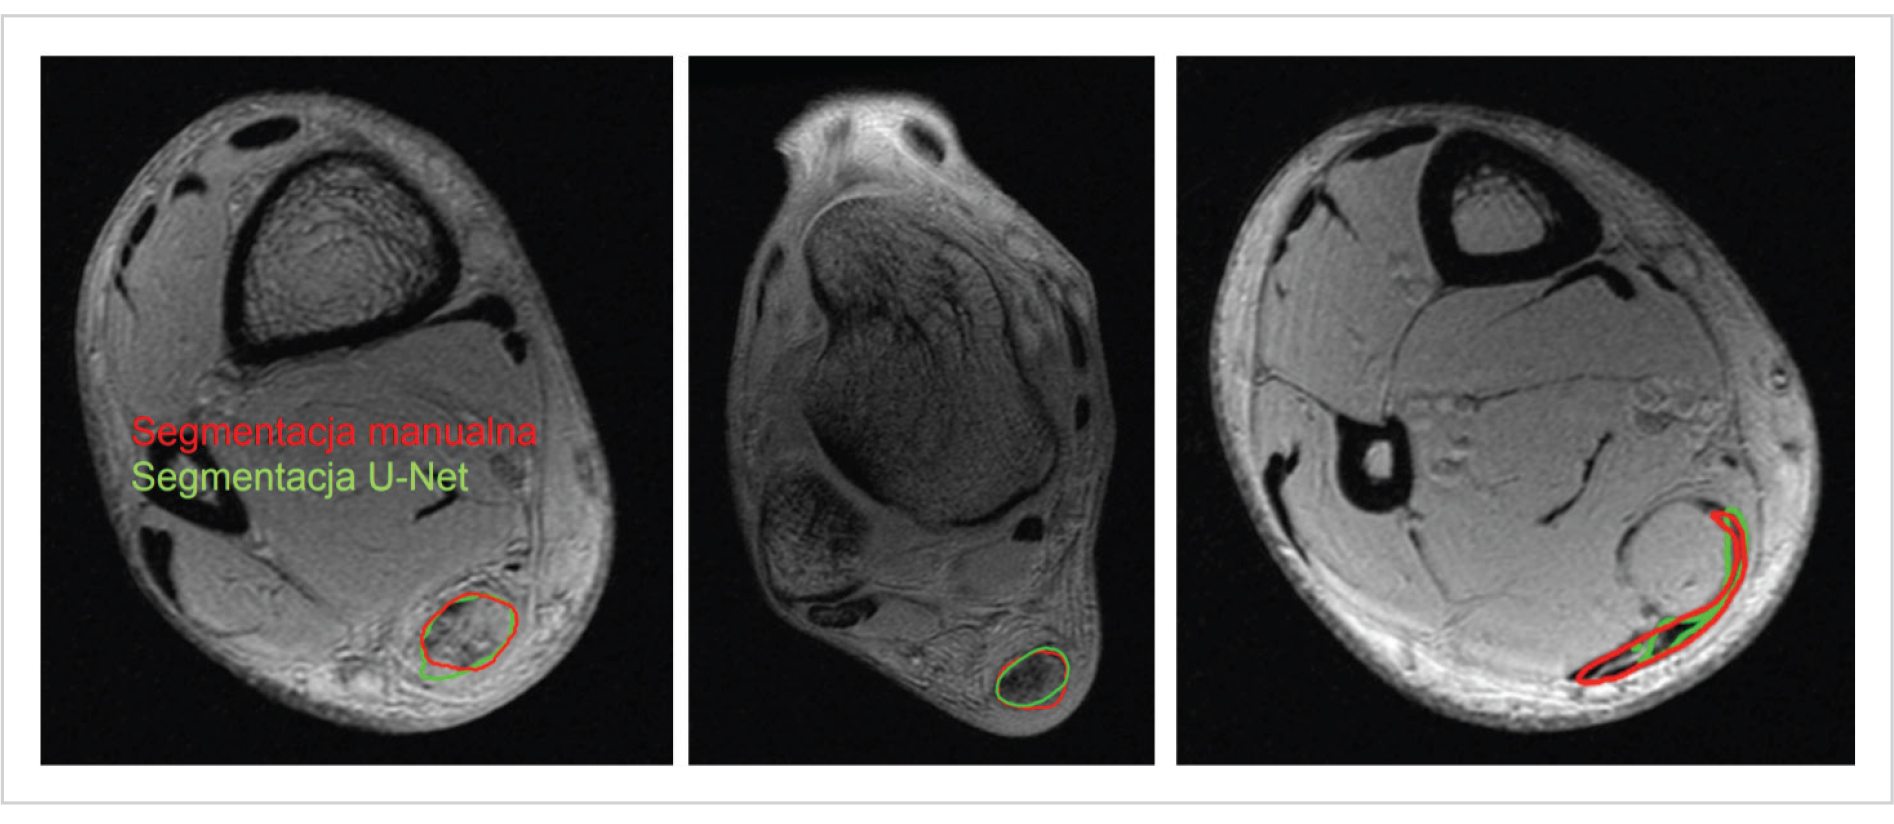
\includegraphics[width=1\textwidth]{figures/Segmentacja.jpg}
	\caption{Automatyczna segmantacja ROI z wykorzystaniem głębokich sieci neuronowych.}\label{fig:segmentacja}
\end{figure}
Kolorem czerwonym oznaczono obszar segmentacji manualnej wykonanej przez eksperta radiologa. Kolorem zielonym efekt segmentacji automatycznej. Miara DICE (zob. \cite{Zou2004}) dla otrzymanych obrazów wynosi około 0,75 i świadczy o wysokiej jakości segmentacji oraz o obiecującym kierunku tego rodzaju prac.

Ciekawym elementem rozwoju automatycznej oceny byłaby również fuzja obu metod tj. podmiana ekstraktora cech DL trenowanego na binarnie oznaczonym zbiorze na ekstraktor uzyskany w modelu Inception-v3$_e$. Jednak z uwagi na omawiane problemy praktyczne z dalszym rozwojem tak utworzonej metody oraz brak obiecujących rezultatów w przeprowadzonych przez autora tej pracy badaniach wstępnych, taka propozycja nie została uwzględniona w prezentowanej rozprawie. 

\section{Porównanie z metodą opartą o dane z USG}
\label{seq:comp-usg}
W tej sekcji opracowana metoda została porównana z automatyczną oceną bazującą na danych z Ultrasonografii. Ponownie, do utworzenia metody opartej o USG, wykorzystano konwolucyjne sieci neuronowe, a dokładniej AlexNet, Inception-v3 i ResNet-50 oraz wykorzystano omówiony w poprzedniej sekcji paradygmat end-to-end. 

Dane dla metody opartej o Ultrasonografię pochodziły również z projektu START. Stosowano się zatem do identycznych odstępów czasowych, co w przypadku badań RM i akwizycji poddano tych samych pacjentów. Z przyczyn praktycznych zmniejszyła się jedynie grupa odniesienia, która w tym przypadku wyniosła 18-stu zdrowych ochotników. Badania zrealizowano z wykorzystaniem aparatu GE 3D high-resolution Voluson E8 Expert z liniową sondą (5--18 MHz). Jako dane wejściowe wykorzystano informacje z trybu B (zob. p. \ref{USG}), których ostateczna liczba wyniosła 565 skanów 3D. 

Dane USG są zbliżone do izotropowych dlatego utworzono zbiory zarówno w oparciu o przekroje w płaszczyźnie osiowej jak i strzałkowej (wykorzystując obrazy, gdzie widoczne jest ścięgno):
\begin{itemize}[noitemsep,nolistsep]
	\item zbiór treningowy USG (strzałkowy) -- zawierał 253.639 2D przekrojów w płaszczyźnie strzałkowej, w tym 245.366 pochodzących od chorych 44-ech pacjentów oznaczonych przez radiologa i 8.273 pochodzących od zdrowych ochotników.
	\item zbiór treningowy USG (osiowy) -- zawierał 467.548 2D przekrojów w płaszczyźnie osiowej, w tym 450.816 pochodzących od chorych 44-ech pacjentów oznaczonych przez radiologa i 16.732 pochodzących od zdrowych ochotników. 
\end{itemize}

Wizualizacja przykładowych danych USG znajduje się na Rys. \ref{fig:US_sample}.
\begin{figure}[h!]
	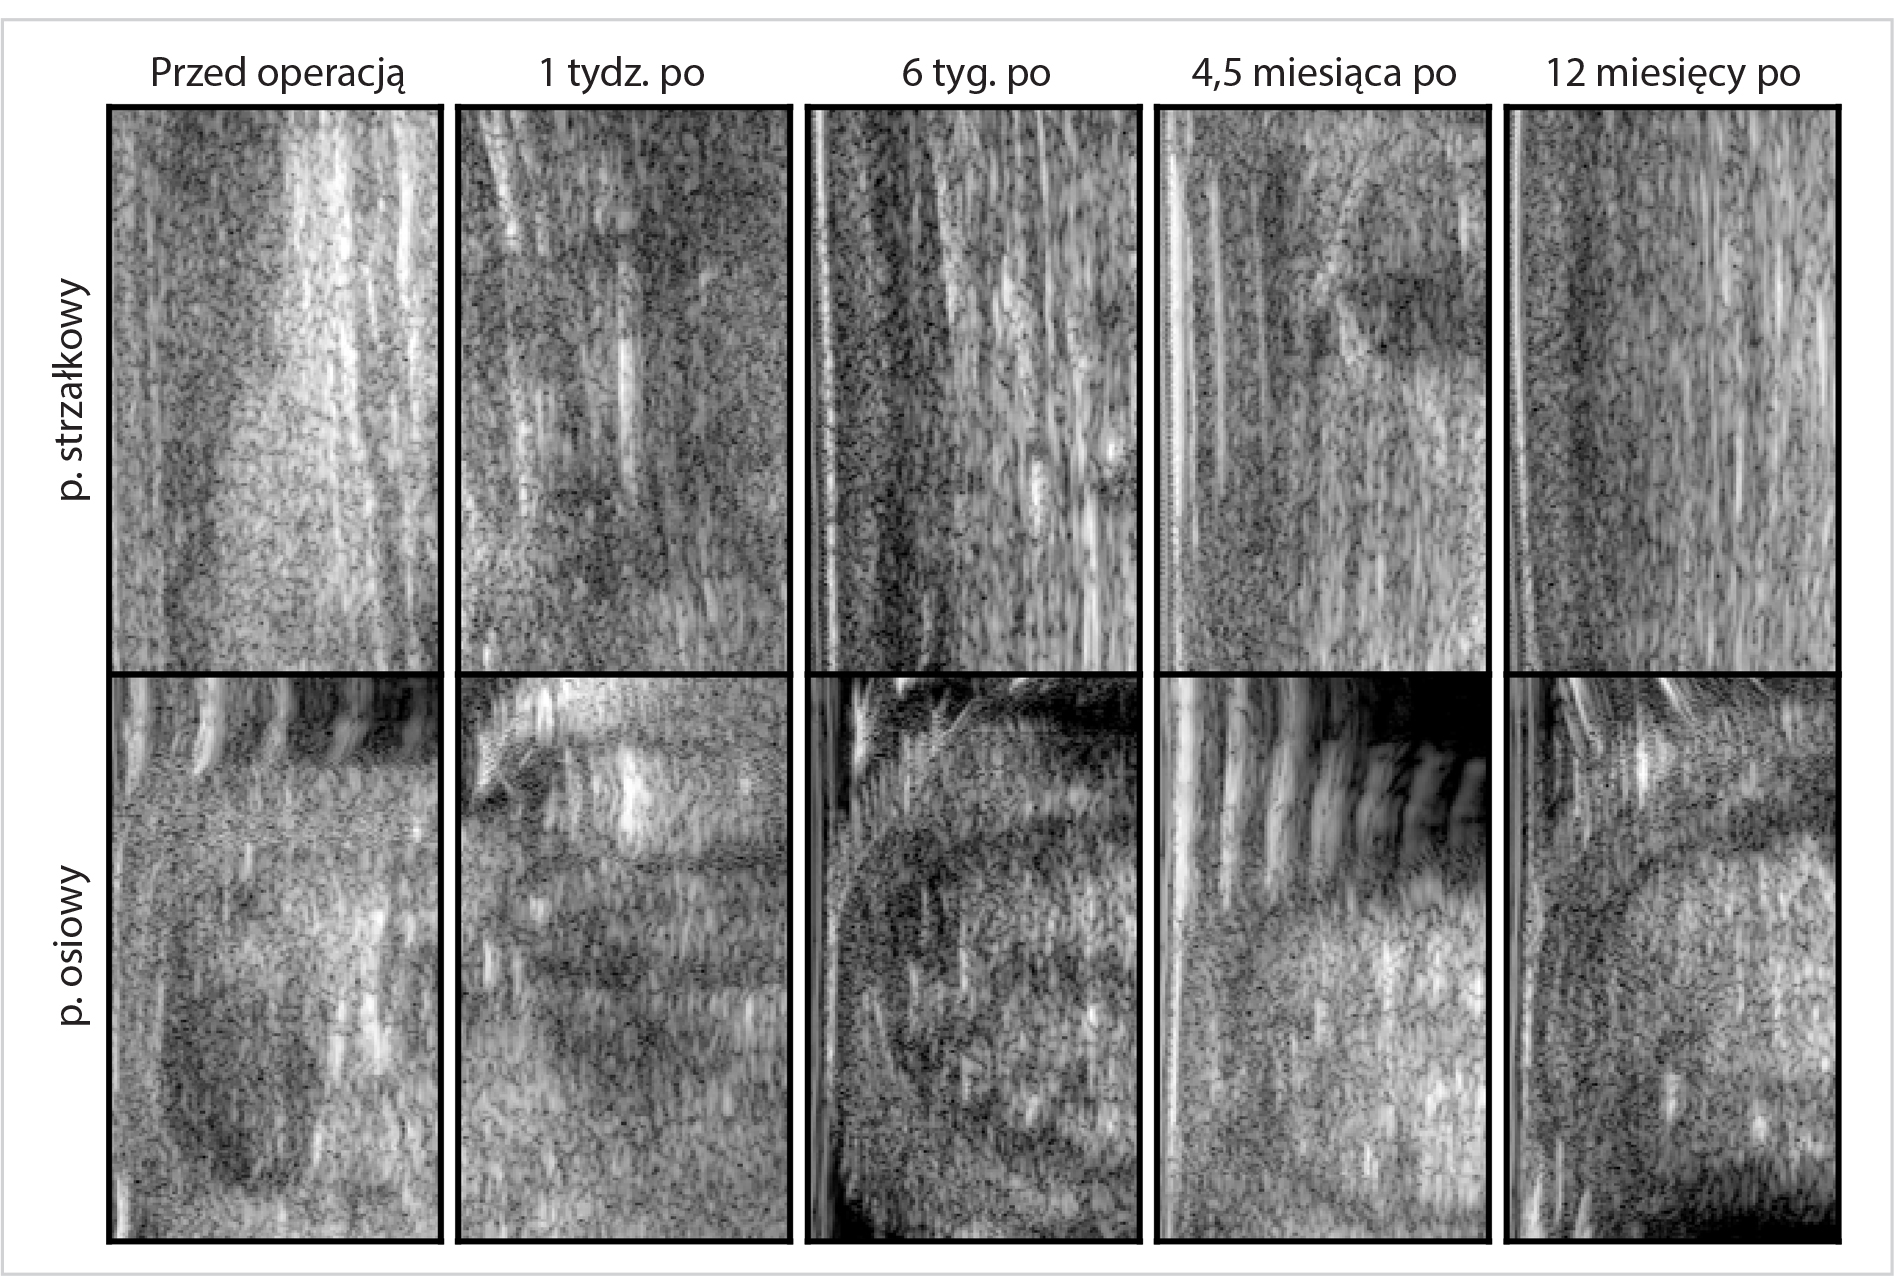
\includegraphics[width=\textwidth]{figures/Data_US_sample.jpg}
	\caption{Wizualizacja przykładowych danych USG w przekrojach osiowych i strzałkowych, w kolejnych tygodniach po zszyciu ścięgna.}
	\label{fig:US_sample}
\end{figure}
W ogólności można zaobserwować ułożenie włókien ścięgnistych na przekrojach strzałkowych i teksturę oraz tkanki otaczające ścięgno na przekrojach osiowych. Jednak szczegółowa analiza załączonych obrazów może być wykonana jedynie przez specjalistę radiologa. 

Utrudniona w stosunku do obrazów RM interpretacja USG ma związek z obecnymi artefaktami w USG i z szumem ziarnistym tworzącym losowe wzorce. Jakość obrazu obniża również jego wartość kliniczną, co wskazują analizy zamieszczone w tej pracy jak i w wielu pracach innych autorów (zob. np. \cite{Khan2003, Ibrahim2013}). Dlatego na początku zdecydowano się przeprowadzić test polegający na prostym zadaniu klasyfikacji binarnej chory/zdrowy (podobnie jak dla badań RM zamieszczonych w Sekcji \ref{binaryMRI}). Ma to na celu porównanie możliwości interpretacji wnioskowania na podstawie obrazów RM i USG. Wyniki dla szkolenia z wykorzystaniem kroswalidacji z 4-ema segmentami zamieszczono w Tabeli \ref{tab:usg-binary}.
\renewcommand{\arraystretch}{1.2}
\begin{table}[]
	\centering
	\scriptsize
	\setlength{\tabcolsep}{3pt}
	\setlength\extrarowheight{2pt}
	\caption{Wyniki szkolenia się sieci dla problemu binarnego na zbiorze treningowym dla danych z USG. Pogrubieniem oznaczono najlepsze wyniki ACC.}
	\label{tab:usg-binary}
	\begin{tabular}{l||c|c|c||c|c|c}
		%\hline
		& \multicolumn{3}{c}{\textbf{p. strzałkowy}} & \multicolumn{3}{c}{\textbf{p. osiowy}} \\
		\textbf{Model} & \textbf{ACC} & \textbf{PPV} & \textbf{TPR} & \textbf{ACC} & \textbf{PPV} & \textbf{TPR} \\ \hline \hline
		AlexNet$_{bu}$ & 0,85$\pm$0,09 & 0,92$\pm$0,08 & 0,78$\pm$0,11 & 0,843$\pm$0,07 & 0,93$\pm$0,06 & 0,73$\pm$0,11  \\ \hline
		Inception-v3$_{bu}$ & \textbf{0,92}$\pm$0,05 & 0,97$\pm$0,04 & 0,90$\pm$0,06 & 0,90$\pm$0,05 & 0,95$\pm$0,03 & 0,87$\pm$0,07 \\ \hline
		ResNet-50$_{bu}$ & 0,91$\pm$0,04 & 0,96$\pm$0,05 & 0,89$\pm$0,08 & \textbf{0,91}$\pm$0,05 & 0,95$\pm$0,04 & 0,88$\pm$0,06 \\ 
	\end{tabular}
\end{table}
\renewcommand{\arraystretch}{1}

Wszystkie modele wytrenowano oddzielnie na przekrojach osiowych i oddzielnie na strzałkowych. Żeby zbalansować dane, przekroje od zdrowych ochotników powiększono poprzez odbicie, a przekroje od chorych pacjentów próbkowano. Dokładność dla najlepszego modelu w przekroju osiowym wyniosła 91,6\%, a w przekroju strzałkowym 91,2\%. Dla porównania, dokładność binarnej klasyfikacji na danych z RM wyniosła 99,83\%. Wyniki te potwierdzają możliwość lepszej interpretacji danych RM dla zadanego problemu, jednak nie dyskryminują USG. W celu polepszenia powyższych rezultatów eksperymentowano również z możliwością klasyfikacji binarnej z wykorzystaniem jedynie obszaru ROI, jednakże działania te przyniosły odwrotny skutek.  
\vspace{10px}
\renewcommand{\arraystretch}{1.2}
\begin{table}[h]
	\scriptsize
	\setlength{\tabcolsep}{3pt}
	\centering
	\caption{Wyniki predykcji oceny gojenia, dla danych z USG, dla pacjentów testowych. Pogrubieniem oznaczono najlepsze rezultaty, osobno dla przekrojów osiowych i strzałkowych}
	\label{tab:usg_train_cross-validation}
	\begin{tabular}{lc||c|c|c|c|c|c}
		%\hline
		& & \multicolumn{6}{c}{\textbf{p. strzałkowy}} \\
		\textbf{Model} & & \textbf{SCT} & \textbf{TT} & \textbf{STE} & \textbf{TE} & \textbf{TU} & \textbf{TisE} \\ \hline \hline
		AlexNet$_{eus}$ & MAE & 0,96$\pm$0,20 & 0,80$\pm$0,13 & 0,82$\pm$0,14 & 0,95$\pm$0,20 & 0,87$\pm$0,20 & 1,08$\pm$0,23  \\
		& MAX-AE & 1,75 & 1,32 & 1,87 & 1,35 & 1,61 & 2,03 \\ 
		& Corr & 0,53 & 0,69 & 0,11 & \textbf{0,68} & 0,31 & 0,22 \\ \hline
		Inception-v3$_{eus}$ & MAE & \textbf{0,88}$\pm$0,16 & \textbf{0,67}$\pm$0,11 & \textbf{0,80}$\pm$0,15 & 0,82$\pm$0,11 & \textbf{0,84}$\pm$0,11 & \textbf{0,93}$\pm$0,15  \\
		& MAX-AE & 1,69 & 1,32 & 1,69 & \textbf{1,31} & \textbf{1,58} & \textbf{1,64} \\ 
		& Corr & \textbf{0,83} & \textbf{0,71} & 0,19 & 0,64 & \textbf{0,56} & \textbf{0,71} \\ \hline
		ResNet-50$_{eus}$ & MAE & 0,89$\pm$0,06 & 0,74$\pm$0,07 & 0,83$\pm$0,11 & \textbf{0,81}$\pm$0,15 & 0,92$\pm$0,15 & 0,99$\pm$0,15 \\
		& MAX-AE & \textbf{1,53} & \textbf{1,22} & \textbf{1,64} & 1,43 & 1,67 & 1,71 \\
		& Corr & 0,62 & 0,38 & \textbf{0,23} & 0,62 & 0,12 & 0,43 \\ \hline \hline
		& & \multicolumn{6}{c}{\textbf{p. osiowy}} \\
		
		AlexNet$_{euo}$ & MAE & \textbf{0,98}$\pm$0,20 & 0,83$\pm$0,16 & 0,82$\pm$0,17 & 0,94$\pm$0,26 & 0,95$\pm$0,25 & 0,86$\pm$0,14  \\
		& MAX-AE & \textbf{1,79} & \textbf{1,36} & 1,86 & 1,41 & 1,61 & 1,59 \\ 
		& Corr & 0,45 & 0,62 & 0,20 & 0,60 & 0,03 & 0,59 \\ \hline
		Inception-v3$_{euo}$ & MAE & 1,03$\pm$0,23 & \textbf{0,70}$\pm$0,12 & \textbf{0,76}$\pm$0,13 & \textbf{0,86}$\pm$0,09 & 0,87$\pm$0,16 & \textbf{0,85}$\pm$0,12  \\
		& MAX-AE & 2,52 & \textbf{1,45} & \textbf{1,45} & \textbf{1,24} & 1,67 & \textbf{1,56} \\ 
		& Corr & \textbf{0,77} & \textbf{0,69} & \textbf{0,22} & \textbf{0,65} & \textbf{0,55} & \textbf{0,72} \\ \hline
		ResNet-50$_{euo}$ & MAE & 1,05$\pm$0,15 & 0,78$\pm$0,16 & 0,80$\pm$0,12 & 1,02$\pm$0,12 & \textbf{0,87}$\pm$0,12 & 0,91$\pm$0,14 \\
		& MAX-AE & 1,98 & 1,51 & 1,59 & 1,63 & \textbf{1,45} & 1,57 \\
		& Corr & 0,52 & 0,47 & 0,21 & 0,64 & 0,18 & 0,57 \\ 
	\end{tabular}
\end{table}
\renewcommand{\arraystretch}{1}

Kolejnym krokiem eksperymentu było porównanie jakości oceny procesu gojenia. W badaniu wykorzystano ponownie paradygmat end-to-end i zmianę warstwy klasyfikującej na regresję z funkcją kosztu określoną jako średni błąd kwadratowy. Dla tej metody próbowano również odtworzyć schemat sprawdzony dla RM, bazujący na treningu binarnym oraz ekstrakcji i redukcji cech. W przypadku USG otrzymane wyniki nie były jednak na tyle satysfakcjonujące, aby zamieszczać je w tej pracy. Ostatecznie, wyniki szkolenia sieci w paradygmacie end-to-end zamieszczono w Tabeli \ref{tab:usg_train_cross-validation}.

Największą liczbę najlepszych rezultatów otrzymano odpowiednio dla modeli na bazie sieci Inception-v3 i ResNet-50 dlatego te modele zostały dalej porównane z proponowaną metodą. W tym celu wyniki MAE, MAX-AE i Corr zostały wyliczone dla zbioru pacjentów testowych i zebrane w Tabeli \ref{tab:USGvsRM-cross-validation}.
\vspace{10px}
\renewcommand{\arraystretch}{1.2}
\begin{table}[h]
	\scriptsize
	\setlength{\tabcolsep}{1pt}
	\centering
	\caption{Porównanie wyników oceny automatycznej, bazującej na danych USG i RM, dla pacjentów ze zbioru testowego. Pogrubieniem oznaczono najlepsze wyniki.}
	\label{tab:USGvsRM-cross-validation}
	\vspace{-0.5cm}
	\begin{tabular}{lc||c|c|c|c|c|c}
		%\hline
		& & \multicolumn{6}{c}{\textbf{USG -- p. strzałkowy}} \\
		\textbf{Model} & & \textbf{SCT} & \textbf{TT} & \textbf{STE} & \textbf{TE} & \textbf{TU} & \textbf{TisE} \\ \hline \hline
		Inception-v3$_{eus}$ & MAE & \textbf{0,81}$\pm$0,19 & 0,63$\pm$0,03 & \textbf{0,56}$\pm$0,09 & 0,85$\pm$0,10 & 0,54$\pm$0,02 & 0,87$\pm$0,14 \\
		& MAX-AE & 1,59 & 1,79 & 1,7 & \textbf{1,25} & \textbf{1,38} & 1,69 \\
		& Corr & 0,80 & 0,77 & 0,31 & 0,52 & \textbf{0,69} & 0,62 \\ \hline
		ResNet-50$_{eus}$ & MAE & 0,88$\pm$0,16 & 0,65$\pm$0,07 & 0,66$\pm$0,04 & 0,83$\pm$0,12 & 0,75$\pm$0,06 & 0,93$\pm$0,11 \\
		& MAX-AE & \textbf{1,49} & \textbf{1,26} & 1,74 & 1,48 & 1,78 & 1,71 \\
		& Corr & 0,60 & 0,55 & 0,25 & 0,55 & 0,34 & 0,56 \\
		\hline \hline
		& & \multicolumn{6}{c}{\textbf{USG -- p. osiowy}} \\
		
		Inception-v3$_{euo}$ & MAE & 0,84$\pm$0,27 & 0,75$\pm$0,7 & 0,58$\pm$0,05 & 0,83$\pm$0,05 & \textbf{0,53}$\pm$0,08 & \textbf{0,83}$\pm$0,15 \\
		& MAX-AE & 2,8 & 1,46 & \textbf{1,51} & 1,27 & 1,63 & 1,65 \\
		& Corr & 0,69 & 0,68 & 0,45 & 0,51 & 0,66 & 0,68 \\ \hline
		ResNet-50$_{euo}$ & MAE & 0,92$\pm$0,18 & 0,76$\pm$0,16 & 0,68$\pm$0,04 & \textbf{0,81}$\pm$0,08 & 0,65$\pm$0,10 & 0,94$\pm$0,05 \\
		& MAX-AE & 2,01 & 1,56 & 1,61 & 1,69& 1,43 & \textbf{1,58}\\
		& Corr & 0,55 & 0,57 & \textbf{0,35} & 0,44 & 0,39 & 0,61 \\ \hline \hline
		& & \multicolumn{6}{c}{\textbf{Rezonans magnetyczny}} \\
		
		SVR & MAE & $1,05\pm0,06$ & \textbf{0,56}$\pm0,03$ & $0,75\pm0,04$ & $0,91\pm0,05$ & $0,91\pm0,04$ & $0,94\pm0,05$\\
		& MAX-AE & 2,62 & 1,82 & 1,92 & 2,54 & 2,01 & 2,38 \\
		& Corr   & \textbf{0,85} & \textbf{0,85} & 0,31 & \textbf{0,72} & 0,65 & \textbf{0,80} \\
		 
	\end{tabular}
\end{table}
\renewcommand{\arraystretch}{1}

Sieć, uzyskująca najlepsze rezultaty, wytrenowana na USG tj. Inception-v3, uzyskała wartości MAE w zakresie $0,53$ do $0,87$ i uśrednioną korelację Z-Fishera od $0,31$ do $0,8$.

Metoda oparta o USG charakteryzuje się lepszymi rezultatami Corr tylko dla parametrów STE i TU, czyli dla parametrów ocenianych przez wzgląd na krawędzie i na oś w płaszczyźnie strzałkowej. W przypadku miary MAE, metoda RM uzyskuje lepszy rezultat w parametrze TT, gdzie znaczący wpływ na ocenę maja cechy z ROI.

Bazując na powyższych rezultatach można wnioskować, że metoda oparta o dane USG może być komplementarna z proponowaną oceną bazującą na danych z RM, zwłaszcza w kontekście oceny parametru TU jak i zmniejszenia błędu MAE w poszczególnych parametrach. Do tego celu potrzebna jest jednak dokładna analiza i zrozumienie podstaw wnioskowania sieci opartej o USG, a następnie wybór oraz realizacja odpowiedniej metody fuzji.

\section{Porównanie z metodą opartą o badania biomechaniczne}
\label{seq:comp-biomechanics}
W tej sekcji opracowana metoda została porównana z wynikami badań biomechanicznych i wynikami funkcjonalnego testu ATRS. Badania te były realizowane w ramach protokołu monitorowania rehabilitacji pacjentów opracowanego w klinice Carolina Medical Center (zob. p. \ref{biomechanika}). 

W ramach projektu START możliwe było zebranie danych dla 30-tu spośród 60-ciu pacjentów. Dane zawierały wyniki pomiaru zrealizowanego w dwóch krokach czasowych tj. w 26-tym i 52-rugim tygodniu po operacji. Po wstępnych analizach, do porównań w tej pracy wykorzystano zebrane wyniki ATRS i deficyty sił mięśniowych będące rezultatem badań biomechanicznych. Dokładniej, określono 16-cie takich deficytów oznaczonych dalej w tej pracy \textit{d1}--\textit{d16}. W czterech pozycjach tj. kolano zgięte i wyprostowane oraz staw skokowy zgięty wyprostowany zrealizowano pomiary w warunkach izometrii i izokinetyki dla trzech prędkości kątowych 60$^\circ$/s, 120$^\circ$/s oraz 180$^\circ$/s  

Z uwagi na dużą liczbę pomiarów, zdecydowano się w pierwszej kolejność na przeprowadzenie analizy czynników głównych i identyfikację nowych zmiennych wyjaśniających w największym stopniu wariancję w zebranym zbiorze danych. Wyniki podsumowano w Tabeli \ref{tab:pca-muscles}.

\begin{table}[h]
	\centering
	\setlength{\tabcolsep}{3pt}
	\setlength\extrarowheight{2pt}
	\caption{Wyniki analizy czynników głównych dla 16-tu pomiarów deficytów mięśniowych w warunkach izometrii i izokinetyki. Oznaczono ładunki, gdzie wartość modułu jest większa niż 0,7.}
	\label{tab:pca-muscles}
	\begin{tabular}{c|c|c|c|c}
		%\hline

		Zmienna&Czynnik1&Czynnik2&Czynnik3&Czynnik4 \\
		\hline \hline
		\textit{d1}&\textbf{-0,77}&0,16&-0,04&-0,25 \\
		\hline
		\textit{d2}&0,32&\textbf{-0,74}&0,038&-0,044 \\
		\hline
		\textit{d3}&\textbf{-0,81}&0,26&-0,17&-0,24 \\
		\hline
		\textit{d4}&0,09&-0,62&-0,50&-0,38 \\
		\hline
		\textit{d5}&\textbf{-0,82}&0,13&-0,03&0,21 \\
		\hline
		\textit{d6}&0,31&-0,53&-0,53&0,42 \\
		\hline
		\textit{d7}&-0,67&-0,20&-0,34&-0,11 \\
		\hline
		\textit{d8}&-0,12&-0,34&-0,67&0,43 \\
		\hline
		\textit{d9}&-0,61&-0,01&-0,28&-0,36 \\
		\hline
		\textit{d10}&0,07&\textbf{-0,84}&0,26&0,02 \\
		\hline
		\textit{d11}&\textbf{-0,81}&-0,14&0,01&0,08 \\
		\hline
		\textit{d12}&-0,11&\textbf{-0,93}&-0,01&-0,01 \\
		\hline
		\textit{d13}&\textbf{-0,72}&-0,24&0,28&0,36 \\
		\hline
		\textit{d14}&-0,12&\textbf{-0,81}&0,33&-0,25 \\
		\hline
		\textit{d15}&-0,58&-0,32&0,39&0,53 \\
		\hline
		\textit{d16}&-0,17&-0,62&0,23&-0,36 \\
		\hline\hline
		Udział&0,28&0,27&0,10&0,09 \\

	\end{tabular}
\end{table}

Z czterech czynników dwa mają wyraźnie większy udział w wyjaśnianej wariancji, osiągając odpowiednio poziomy 28 i 27\%. Istotne jest również, że trzy z pięciu znaczących ładunków czynnikowych (\textit{d1}, \textit{d3}, \textit{d5}) dla pierwszego czynnika znajdują się w przedziale \textit{d1}--\textit{d8}, które skojarzone są z pozycją kolana prostego oraz, że dla drugiego czynnika głównego sytuacja jest odwrotna i trzy z czterech ładunków czynnikowych (\textit{d10}, \textit{d12}, \textit{d14}) znajdują się w przedziale \textit{d9}--\textit{d16}, czyli badania przy kolanie zgiętym. 

Co oczywiste, pozycja kolana wpływa znacząco na wynik badania biomechanicznego, dlatego w ramach dalszej pracy zdecydowano się na  analizę czynnikową dla wyprostowanego i zgiętego kolana oddzielnie. Wyniki zostały przedstawione w Tabeli \ref{tab:pca-muscles-knee-strait-bended}. 

Ponownie można zaobserwować charakterystyczne rozróżnienie. Pierwszy czynnik główny dla badania w pozycji kolana wyprostowanego zawiera ładunki znaczące o nieparzystych numerach, a drugi czynnik posiada znaczące ładunki o parzystych numerach. W przypadku badania w pozycji kolana zgiętego sytuacja jest odwrotna i analogicznie można zaobserwować rozróżnienie. W tym przypadku podział wynika z pozycji stawu skokowego. Ładunki o nieparzystych numerach posiadają czynniki związane z badaniami w zgięciu stawu skokowego, a o parzystych w wyproście. Z uwagi na ten fakt do kolejnych porównań zostały zdefiniowane następujące 4 zmienne:
\begin{enumerate}[noitemsep,nolistsep]
	\item $ZZ$ -- wyniki dla pozycji kolano zgięte i staw skokowy zgięty.
	\item $ZW$ -- wyniki dla pozycji kolano zgięte i staw skokowy wyprostowany.
	\item $WZ$ -- wyniki dla pozycji kolano wyprostowane i staw skokowy zgięty.
	\item $WW$ -- wyniki dla pozycji kolano wyprostowane i staw skokowy wyprostowany.
\end{enumerate} 
\begin{table}[h!]
	\centering
	\setlength{\tabcolsep}{3pt}
	\setlength\extrarowheight{2pt}
	\caption{Wyniki analizy czynników głównych dla 16-tu pomiarów deficytów mięśniowych, oddzielnie dla pozycji kolana zgiętego i wyprostowanego. Oznaczono ładunki, gdzie wartość modułu jest większa niż 0,7.}
	\label{tab:pca-muscles-knee-strait-bended}
	\begin{tabular}{c|c|c||c|c|c}
		%\hline
		
		Zmienna&Czynnik1&Czynnik2&Zmienna&Czynnik1&Czynnik2 \\
		\hline \hline
		\textit{d1}&\textbf{-0,82}&-0,14&d9&-0,26&0,64 \\
		\hline
		\textit{d2}&-0,60&-0,37&d10&\textbf{-0,72}&-0,47 \\
		\hline
		\textit{d3}&\textbf{0,88}&-0,20&d11&-0,52&\textbf{0,73} \\
		\hline
		\textit{d4}&-0,36&-0,65&d12&\textbf{-0,83}&-0,34 \\
		\hline
		\textit{d5}&\textbf{0,83}&-0,26&d13&-0,65&0,64 \\
		\hline
		\textit{d6}&-0,57&-0,64&d14&\textbf{-0,81}&-0,43 \\
		\hline
		\textit{d7}&0,55&-0,60&d15&-0,67&0,40 \\
		\hline
		\textit{d8}&-0,03&\textbf{-0,80}&d16&-0,65&-0,38 \\
		\hline\hline
		Udział&0,41&0,26&&0,44&0,27 \\
		
	\end{tabular}
\end{table}

Każda z nowo powstałych zmiennych składa się z czterech pomiarów: jednego dla izometrii i trzech dla izokinetyki. Dokładne zestawienie znajduje się w Tabeli \ref{tab:bio-new-factors}.
\vspace{20px}
\begin{table}[h!]
	\centering
	\setlength{\tabcolsep}{3pt}
	\setlength\extrarowheight{2pt}
	\caption{Komponenty i ich udział, wchodzące w skład nowych zmiennych opisujących biomechanikę.}
	\label{tab:bio-new-factors}
	\begin{tabular}{c|c|c|c|c||c}
		Zmienna&Czynnik1&Czynnik2&Czynnik3&Czynnik4&Udział \\
		\hline \hline
		$ZZ$&\textit{d9} (-0,61)&\textit{d11} (-0,88)&\textit{d13} (-0,92)&\textit{d15} (-0,77)&0,65\\
		\hline
		$ZW$&\textit{d10} (-0,86)&\textit{d12} (-0,91)&\textit{d14} (-0,92)&\textit{d16} (-0,77)&0,75\\
		\hline
		$WZ$&\textit{d1} (-0,85)&\textit{d3} (-0,90)&\textit{d5} (-0,87)&\textit{d7} (-0,72)&0,70\\
		\hline
		$WW$&\textit{d2} (-0,64)&\textit{d4} (-0,76)&\textit{d6} (-0,88)&\textit{d8} (-0,66)&0,55\\
		
		
	\end{tabular}
\end{table}

Taki podział wydaje się być intuicyjny, ale fakt otrzymania powyższych wyników w analizie numerycznej jest wartością dodaną potwierdzającą spójność danych i jakość przeprowadzonych badań przez fizjoterapeutów z Carolina Medical Center. 

W celu efektywnego porównania nowych zmiennych opisujących biomechanikę ścięgna i wyniku ATRS z predykcjami automatycznej metody oraz oceną radiologa, zdecydowano się również dla badań radiologicznych przeprowadzić analizę czynnikową. W obu przypadkach tj. oceny automatycznej i radiologa uzyskano minimalny udział w wyjaśnianej wariancji czynników innych niż pierwszy. Stąd możliwość wprowadzenia nowej zmiennej tj. Czynnik1 zamiast 6-ciu parametrów: $SCT$, $STE$, $TE$, $TisE$, $TT$, $TU$. Szczegółowe wyniki znajdują się w Tabeli \ref{tab:pca-gt-pred}.

\begin{table}[h]
	\centering
	\setlength{\tabcolsep}{3pt}
	\setlength\extrarowheight{2pt}
	\caption{Rezultaty analizy czynników głównych dla oceny radiologicznej i oceny automatycznej realizowanych z wykorzystaniem 6-ścio parametrycznej ankiety. Oznaczono ładunki, gdzie wartość modułu jest większa niż 0,7.}
	\label{tab:pca-gt-pred}
	\begin{tabular}{c|c|c}
		Zmienna&Czynnik1 - ocena radiologa&Czynnik1 - ocena automatyczna \\
		\hline \hline
		SCT&\textbf{-0,79}&\textbf{-0,95}\\
		\hline
		STE&0,57&\textbf{0,86}\\
		\hline
		TE&\textbf{-0,85}&\textbf{-0,94}\\
		\hline
		TisE&\textbf{-0,71}&\textbf{-0,89}\\
		\hline
		TT&\textbf{-0,76}&\textbf{-0,72}\\
		\hline
		TU&\textbf{-0,88}&\textbf{-0,94}\\
		\hline \hline	
		Udział&0,57&0,78\\
			
	\end{tabular}
\end{table}

Można zaobserwować, że udział wyjaśnianej wariancji w pierwszym czynniku jest większy dla oceny automatycznej niż dla oceny radiologa. Subiektywna ocena eksperta wprowadza nieuniknioną niepewność do pomiaru, stąd wyniki generowane przez człowieka są w większym stopniu losowe niż wyniki oceny automatycznej. 

W kolejnych badaniach zestawione zostały interkorelacje nowych zmiennych. W Tabeli \ref{tab:gtVSpred}, przedstawiono korelację oceny automatycznej z oceną radiologa.

\vspace{10px}
\begin{table}[h]
	\centering
	\setlength{\tabcolsep}{3pt}
	\setlength\extrarowheight{2pt}
	\caption{Korelacja między oceną radiologa, a ocena automatyczną. Oznaczone wsp. korelacji są istotne z $p$ $<$ 0,05 dla $N$=30.}
	\label{tab:gtVSpred}
	\begin{tabular}{c|c|c}
		&Ocena automatyczna &Ocena radiologa \\
		\hline \hline
		Ocena automatyczna&1,0000&\textbf{0,8070}\\
		\hline
		Ocena radiologa&\textbf{0,8070}&1,0000\\
			
	\end{tabular}
\end{table}

Naturalnie, nowa zmienna opisująca ocenę radiologa koreluje z nową zmienną opisującą ocenę automatyczną. Fakt ten jest kolejnym potwierdzeniem na silny związek między zastosowanymi metodami przetwarzania obrazów i eksperckimi, ludzkimi spostrzeżeniami. 

W kolejnej tabeli (tj. Tabeli \ref{tab:bioVSatrs}) przedstawiono wyniki korelacji nowych zmiennych opisujących biomechanikę z wynikami testu ATRS. 
\vspace{10px}
\begin{table}[h]
	\centering
	\setlength{\tabcolsep}{3pt}
	\setlength\extrarowheight{2pt}
	\caption{Korelacja badań biomechanicznych z testem ATRS. Oznaczone wsp. korelacji są istotne z $p$ $<$ 0,05 dla $N$=30.}
	\label{tab:bioVSatrs}
	\begin{tabular}{c|c|c|c|c|c}
		&WW&WZ&ZW&ZZ&ATRS \\
		\hline \hline
		WW&1,0000&-0,2037&\textbf{0,4948}&-0,0436&-0,2190\\
		\hline
		WZ&-0,2037&1,0000&-0,0143&\textbf{0,5815}&0,1070\\
		\hline
		ZW&\textbf{0,4948}&-0,0143&1,0000&0,2324&-0,2620\\
		\hline
		ZZ&-0,0436&\textbf{0,5815}&0,2324&1,0000&0,1437\\
		\hline
		ATRS&-0,2190&0,1070&-0,2620&0,1437&1,0000\\
		
		
	\end{tabular}
\end{table}

Można zaobserwować istotną korelację pomiarów wykonanych przy takim samym ustawieniu kolana. Jest to istotniejsze nawet od ustawienia stawu skokowego. Z kolei analizując rezultaty korelacji z ATRS, można zaobserwować słabą korelację z wynikami pomiarów biomechanicznych. Wynik wskazuje, że uzasadnione jest realizowanie w praktyce obydwu tych badań w celu skuteczniejszego monitorowania rehabilitacji pacjentów.

Finalnie, zestawiono nowe zmienne opisujące ocenę radiologa i ocenę automatyczną, z wynikami badań biomechanicznych i ATRS. Szczegółowe rezultaty przedstawiono w Tabeli \ref{tab:bioATRSvspredGT}.
\vspace{10px}
\begin{table}[h]
	\centering
	\setlength{\tabcolsep}{3pt}
	\setlength\extrarowheight{2pt}
	\caption{Korelacja badań biomechanicznych i testu ATRS z badaniami radiologicznymi ocenionymi automatycznie i przez radiologa. Oznaczone wsp. korelacji są istotne z $p$ $<$ 0,05 dla $N$=30.}
	\label{tab:bioATRSvspredGT}
	\begin{tabular}{c|c|c}
		&ocena automatyczna&ocena radiologa \\
		\hline \hline
		WW&0,1197&0,0706\\
		\hline
		WZ&0,1576&0,1931\\
		\hline
		ZW&0,3429&0,3092\\
		\hline
		ZZ&0,3100&0,2996\\
		\hline
		ATRS&\textbf{0,3854}&0,2088\\
		
	
	\end{tabular}
\end{table}

Można zaobserwować, że wskazania radiologa słabo korelują z wynikami badań biomechanicznych oraz ATRS, co jest zgodne z praktyką kliniczną -- dlatego zalecane jest wykonywanie badań radiologicznych, które dostarczając komplementarnych informacji.

Interesującym rezultatem jest wynik istotnej, niewielkiej korelacji oceny automatycznej z ATRS. Można wnioskować, że eliminacja losowości wynikającej z czynnika ludzkiego, spowodowała usystematyzowanie oceny i uwspólnienie pewnych informacji, które obecne są również w ustrukturyzowanym teście ATRS. Wynik ten wyznacza ciekawy kierunek dalszych prac, mających na celu stworzenie komplementarnego testu maksymalizującego informację dla lekarza prowadzącego, przy jednoczesnym minimalizowaniu objętości protokołu monitorowania pacjentów.

\chapter{Podsumowanie}

W ramach pracy osiągnięto wszystkie założone we wstępie cele. Cel główny tj. opracowanie automatycznej metody oceny gojenia się ścięgna Achillesa został osiągnięty poprzez zastosowanie unikalnej fuzji cech wyuczonych przez model głębokiej sieci neuronowej i cech wyekstrahowanych z wykorzystaniem klasycznych metod przetwarzania obrazów. Wnioski zostały spisane w Rozdziale \ref{NewMethod} podzielonym na trzy sekcje. W pierwszej (p. \ref{seq:method}), przedstawiono szczegółowy opis komponentów oraz ich parametrów wraz z unikalnymi w skali światowej danymi. W drugiej (p. \ref{seq:experiments}), zaprezentowano wyniki eksperymentów mających na celu dobór komponentów i ich parametrów oraz optymalizację czasu, jakości i kosztów związanych z zastosowaniem nowej metody. W ostatniej (p. \ref{seq:valuation}), trzeciej sekcji zaprezentowano szczegółową walidację wraz z analizą rozbieżności między nowym podejściem, a oceną radiologa.

W toku prac, zrealizowano również wszystkie cztery cele szczegółowe. Pierwszy, tj. "Wybór efektywnego kosztowo i czasowo protokołu badania bazującego na technikach obrazowania medycznego, a dokładniej Rezonansu Magnetycznego" zrealizowano poprzez badania zamieszczone w p. \ref{seq:protocol_selection}. Najważniejszym rezultatem tych prac jest określenie utylitarnego protokołu badania składającego się tylko z jednej, trwającej około 5 min. sekwencji RM. 

Drugi cel, tj. "Przetestowanie różnego rodzaju podejść związanych ze szkoleniem głębokich sieci neuronowych" zrealizowano poprzez zestawienie wyników działania nowej metody z wynikami alternatywnego podejścia tj. szkolenia sieci w oparciu o paradygmat end-to-end (zob. p. \ref{seq:end-to-end}). W zestawieniu z alternatywną metodą analizy obrazów RM, wykazano przewagę zaproponowanego podejścia, a dokładniej uzyskano lepsze rezultaty korelacji w każdym z sześciu ocenianych parametrów oraz dla czterech z nich, niższy absolutny błąd średni.

Kolejny cel, tj. "Porównanie wyników oceny nowej metody z wynikami klasyfikacji bazującej na danych z ultrasonografii" zrealizowano dołączając do pracy wyniki automatycznej interpretacji obrazów USG (zob. p. \ref{seq:comp-usg}). W szczególności wykazano możliwość synergii obu podejść, bazując na większej izotropowości danych USG i dobrych wynikach oceny parametrów widocznych w płaszczyźnie strzałkowej.

Ostatni cel, tj. "Porównanie wyników oceny nowej metody z oceną funkcjonalną, rutynowo stosowana do wspomagania rehabilitacji po urazie ścięgna" osiągnięto uzyskując unikalne dane pomiarów biomechanicznych i testu ATRS, a następnie zestawiając je z wynikami nowo-opracowanej metody (zob. p. \ref{seq:comp-biomechanics}). Pokazano przydatność wykonywania badań radiologicznych, przez wzgląd na odmienność niesionej informacji. Jednocześnie określono potencjalny obszar optymalizacji w zakresie niewielkiej, ale istotnej korelacji proponowanej oceny automatycznej z wynikami testu ATRS.  

W ramach powyższych prac nad nowym podejściem do oceny procesu gojenia się ścięgna Achillesa w badaniach RM, całość zadań dotyczących głębokich sieci neuronowych została zrealizowana przez autora tej pracy. Pełnił on również rolę głównego badacza, projektując i współrealizując prace nad fuzją cech (w szczególności w ramach testów perceptronu wielowarstwowego i SVR jako typów meta-regresji). Autor tej pracy również nadzorował i planował eksperymenty grupy tworzącej metody bazujące na paradygmacie end-to-end oraz wykorzystywane do interpretacji obrazów USG. Następnie samodzielnie dokonał ich porównania z proponowanym w tej pracy podejściem. 

Wszystkie wyniki mają charakter innowacyjny. Nie istnieje obecnie, wedle najlepszej wiedzy autora tej pracy, alternatywne podejście do usystematyzowanej i wyliczanej automatycznie oceny stanu gojenia się ścięgna Achillesa widocznego w badaniach RM. Rozprawa ta stanowi zatem kompleksowy opis obecnego \textit{state-of-the-art} dla przedmiotowego problemu. Biorąc pod uwagę, że w przedstawionym stanie najlepsze wyniki oceny automatycznej korelują z oceną radiologa na poziomie 0,85, a minimalny uzyskany absolutny błąd średni równy jest 0,56, krytyczne w opinii autora tej pracy staje się polepszenie wzorca odniesienia. 

Planowana jest zatem dalsza, stała współpraca z radiologami i decydentami celem realizacji ocen przez kolejnych specjalistów oraz wieloośrodkowe zbieranie nowych wolumenów danych. Przewidziane jest także przeprowadzenie badań w zakresie usprawnienia przetwarzania danych, w szczególności w kwestii automatycznej segmentacji ROI. Zrealizowane prace stanowią również fundament pod rozpoczęcie nowych testów, dotyczących pokrewnych zadań, jak ocena gojenia się podobnych struktur np.: więzadeł stawu kolanowego, skokowego, barkowego, czy łokciowego. 

Polepszenie skuteczności wspomagania rehabilitacji w obszarze układu mięśniowo-szkieletowego stanowi według autora tej pracy ciekawe wyzwanie badawcze, jak również ma wymiar praktyczny. Już teraz bowiem, według danych Krajowej Izby Fizjoterapeutów, po zwolnieniach z pracy dotyczących ciąży, zwolnienia na skutek dolegliwości mięśniowo-szkieletowych stanowią drugi powód absencji w pracy w Polsce. W odpowiedzi na rosnący problem, w ramach otrzymanego przez autora tej pracy i mgr. Bartosza Boruckiego w Czerwcu 2019 roku grantu z programu Inkubator Innowacyjności 2.0, organizowanego przez ministra nauki i szkolnictwa wyższego, planowana jest realizacja wyżej wymienionych prac i przygotowanie do wdrożenia przedmiotowego rozwiązania. Działania pozwolą na usprawnienie rehabilitacji ścięgna Achillesa oraz jego profilaktyki, jak i rozpoczęcie badań nad opracowaniem rozwiązań dedykowanych dla wspomagania leczenia innych, podobnych urazów.


%- jeden radiolog więc ankieta ok
%- AlexNet uczy się bardziej generycznych cech niż ResNet, który zwraca uwagę na szczególy: https://www.researchgate.net/post/Can_AlexNet_be_a_better_feature_extractor_than_ResNet

%https://icmlviz.github.io/icmlviz2016/assets/papers/4.pdf

%Wydzielenie stanu przed operacją i oznaczenie osobną etykietą w procesie treningu mogłoby doprowadzić do polepszenia rezultatu, co jest sugestią dla przyszłych prac związanych z rozwojem metody.

%TU - Polepszenie w zakresie oceny tego parametru może być uzyskane w przypadku zastosowania bardziej jednorodnych danych RM lub USG.




%   this is for BibTeX.  remove if you plan to write the references in the document
\bibliographystyle{plplain}
\bibliography{refs}

%adds the bibliography to the table of contents
\addcontentsline{toc}{chapter}
         {\protect\numberline{Bibliografia\hspace{-96pt}}}
         
%dodatki
\appendix
%\chapter{Symbole przyjęte w pracy}
%\label{app:symbole}

%Jeśli w tekście nie wykazano inaczej, stosowane symbole należy rozumieć jako:

%\begin{itemize}
%\item[$f(x,y)$] - jasność piksela o współrzędnych $(x,y)$ w obrazie wejściowym,
%\item[$g(x,y)$] - jasność piksela o współrzędnych $(x,y)$ w obrazie wynikowym,
%\item[$t$, $t_i$] - wartości progowe,
%\item[$G$] - liczba poziomów szarości obrazu; $G=256$,
%\item[$P(i,j)$] - macierz GLCM,
%\item[$M(i,j)$] - maska przetwarzania.
%\end{itemize}


%%%%%%%%%%%%%%%%%%%%%%%%%%%%%%%%%%%%%%%%%%%%%%%%%%%%%%%%
\chapter{AchillesDL: System komputerowego wspomagania oceny gojenia ścięgien i więzadeł}
\label{app:AchillesDL}

\begin{figure}[]
	\centering
	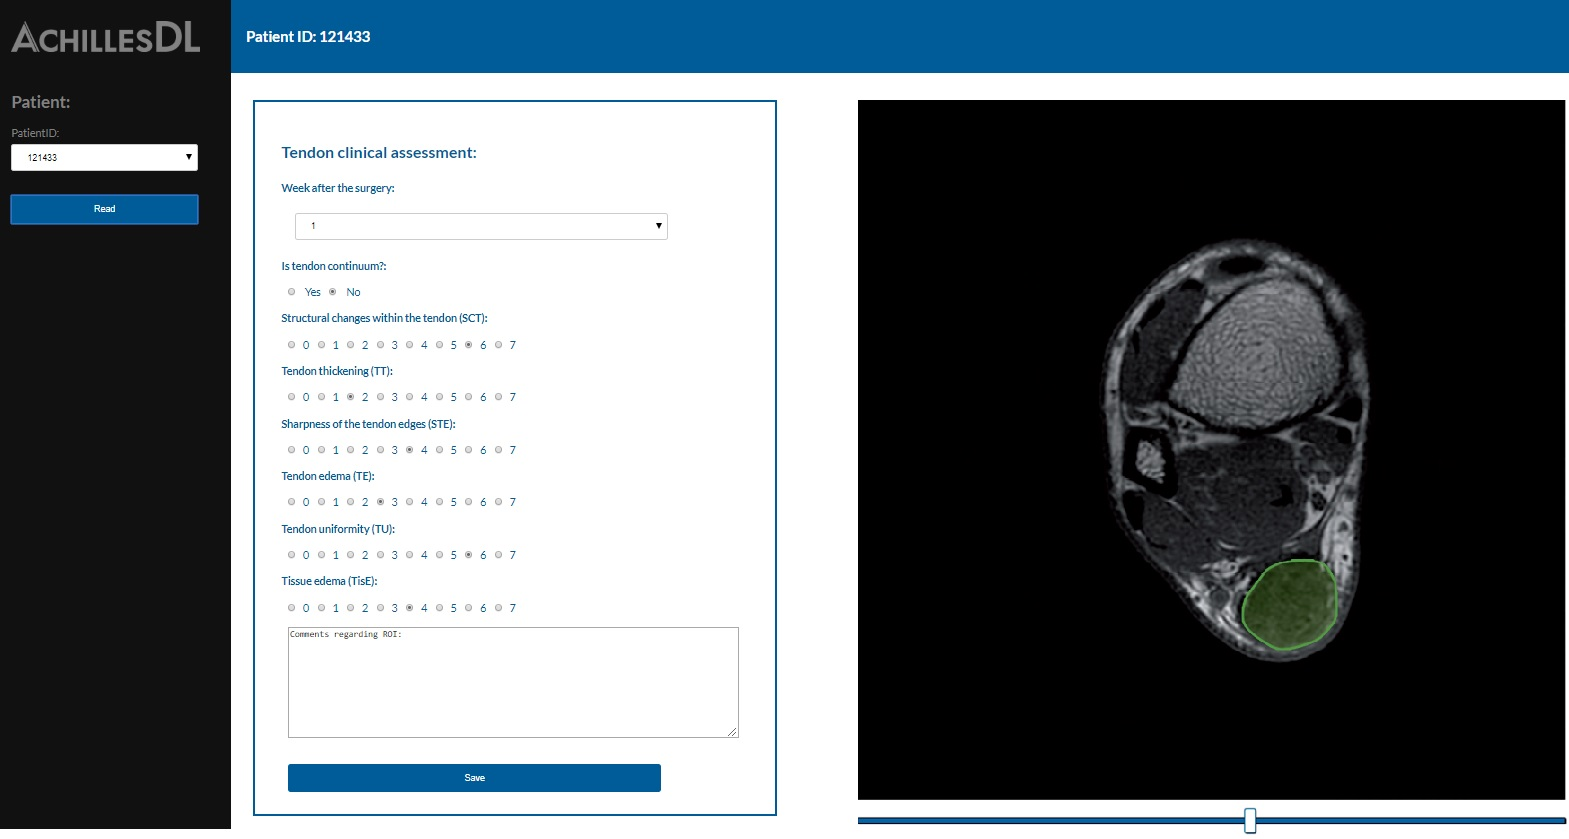
\includegraphics[width=1\textwidth]{figures/achillesDL.jpg}
	\caption{Front-end aplikacji internetowej AchillesDL przeznaczonej do oznaczania  badań RM ścięgna Achillesa.}\label{fig:achillesDL}
\end{figure}

\end{document}